\documentclass[6pt]{jreport}

\usepackage{amsmath,amssymb,amscd}
\usepackage[obeyspaces]{url}
\usepackage[all]{xy}
\usepackage{multicol}
\usepackage{stmaryrd}
\usepackage{float}
%\usepackage{sty/thmbox}
\usepackage{sty/cprog}
\usepackage{sty/simplewick}
\usepackage{sty/braket}
\usepackage{sty/boxedminipage}
\usepackage{sty/algorithm}
\usepackage{sty/algorithmicx}
\usepackage{sty/algpseudocode}
%\usepackage{sty/multirow}
\usepackage{sty/bigdelim}
\usepackage{sty/youngtab}
\usepackage[dvipdfm]{color}
\usepackage[dvipdfm,dvips]{graphicx}
\usepackage[dvipdfm %
  , colorlinks=true %
  , bookmarks=true %
  , bookmarksnumbered=false %
  , bookmarkstype=toc %
  , pdfkeywords={TeX; dvipdfmx; hyperref; color;} %
	]{hyperref}
\ifnum 42146=\euc"A4A2 
  \AtBeginDvi{\special{pdf:tounicode EUC-UCS2}}% platex-utf8 でも OK
\else
  \AtBeginDvi{\special{pdf:tounicode 90ms-RKSJ-UCS2}}%"
\fi
%
%theorem
%
%\newtheorem[S]{theorem}{定理}[section]
%\newtheorem[S]{proposition}{命題}[section]
%\newtheorem[S]{corollary}{系}[section]
%\newtheorem[S]{lemma}{補題}[section]
%\newtheorem[S]{definition}{定義}[section]
%\newtheorem[S]{example}{例}[section]
%\newtheorem[S]{conjecture}{予想}[section]
%\newtheorem[S]{problem}{問題}[section]
%\newtheorem[S]{observation}{観察}[section]
%\newtheorem[S]{formula}{公式}[section]
%\newtheorem[S]{todo}{課題}[section]
%\newtheorem[S]{notation}{記法}[section]
%\newtheorem[S]{note}{ノート}[section]
%
\usepackage{sty/shadethm}
%\newshadetheorem[S]{theorem}{定理}[section]
\newshadetheorem{proposition}{命題}[section]
%\newshadetheorem[S]{corollary}{系}[section]
%\newshadetheorem[S]{lemma}{補題}[section]
\newshadetheorem{definition}{定義}[section]
\newshadetheorem{example}{例}[section]
%\newshadetheorem[S]{conjecture}{予想}[section]
%\newshadetheorem[S]{problem}{問題}[section]
\newshadetheorem{problem}{問題}[section]
%\newshadetheorem[S]{observation}{観察}[section]
%\newshadetheorem[S]{formula}{公式}[section]
\newshadetheorem{notation}{記法}[section]
\newshadetheorem{todo}{課題}[section]
\newshadetheorem{note}{ノート}[section]
\newshadetheorem{procedure}{手順}[section]
%
\def\proof{\rm \trivlist \item[\hskip \labelsep{証明}] }
\def\endproof{{\large$\Box$}\endtrivlist}
%
%symbols
%
\newcommand{\zettai}[1]{\left|{#1}\right|}
%\newcommand{\mynorm}[1]{\left\lVert{#1}\right\rVert}
\newcommand{\kakko}[1]{\left({#1}\right)}
\newcommand{\bakko}[1]{\left[{#1}\right]}
\newcommand{\bou}{\;\vert\;}
\newcommand{\myop}[1]{\operatorname{#1}}
\newcommand{\mybf}[1]{{\mathbf{#1}}}
\newcommand{\mycal}[1]{{\mathcal{#1}}}
\def\obra#1{\mathinner{({#1}|}}
\def\oket#1{\mathinner{|{#1})}}
\def\obraket#1{\mathinner{({#1})}}
\newcommand{\jump}[1]{\ensuremath{[\![#1]\!]}}
\newcommand{\myor}{\,\operatorname{or}\,}
\newcommand{\myxor}{\,\operatorname{xor}\,}
\newcommand{\myand}{\,\operatorname{and}\,}
\newcommand{\myspace}{\text{\textvisiblespace}}
%\newcommand{\mybinom}[2]{\left[{{#1}\atop{#2}}\right]}
\newcommand{\mybinom}[2]{\genfrac{[}{]}{0pt}{1}{#1}{#2}}
\newcommand{\myhere}{\mathchar`-}
\newcommand{\mybiop}[1]{\mathchar`-{#1}\myhere}
%obsolete
%\newcommand{\mypowop}[1]{\myhere^{#1}}
\newcommand{\lcomment}[1]{//\;\text{#1}}
%
%category
%
\newcommand{\homset}{\myop{hom}}
\newcommand{\mapset}{\myop{map}}
\newcommand{\myid}{{\myop{id}}}
\newcommand{\mydu}{{\myop{du}}}
%\newcommand{\curry}{\myop{curring}}
%\newcommand{\mycat}[1]{{\mathbf{#1}}}
%
%tree
%
%\newcommand{\raisexy}[1]{\raisebox{\depth}[\totalheight][0pt]{\xymatrix{#1}}}
\newcommand{\mytree}[1]{\raisebox{0.4\totalheight}{\xymatrix@R=4pt@C=1pt{#1}}}
%
%program
%
%\newcommand{\hankukan}[2]{{#1}\lhd{#2}}
%\newcommand{\mysign}{\operatorname{sign}}
%\newcommand{\bnfletter}[1]{\operatorname{#1}}
%\newcommand{\bnfword}[1]{\braket{\operatorname{#1}}}
%\newcommand{\bnfaction}[1]{\bakko{\operatorname{#1}}}
\newcommand{\bool}{\mybf{B}}
\newcommand{\sizen}{\mybf{N}}
\newcommand{\sei}{\mybf{Z}}
\newcommand{\jitu}{\mybf{R}}
\newcommand{\fukuso}{\mybf{C}}
%
\usepackage{sty/accents}
\makeatletter
\def\widebar{\accentset{{\cc@style\underline{\mskip10mu}}}}
\makeatother
\renewcommand{\bar}[1]{\widebar{#1}}
%
%arrows
%The“number”0395 after \ext@arrow defines the position
%relative to the extended error and is not a number but four parameters
%for additional space in the math unit mu. mu is defined as the followings:
%1st digit: space left
%2nd digit: space right
%3rd digit: space left and right
%4th digit: space relativ to the tip of the “arrow”
%
\makeatletter
\def\xmapstofill@{%
	\arrowfill@{\mapstochar\relbar}\relbar\rightarrow%
}
\newcommand*\xmapsto[2][]{%
	\ext@arrow 0395\xmapstofill@{#1}{#2}%
}
\def\xmapsfromfill@{%
	\arrowfill@\leftarrow\relbar{\relbar\mapstochar}%
}
\newcommand*\xmapsfrom[2][]{%
	\ext@arrow 0395\xmapsfromfill@{#1}{#2}%
}
\def\xMapstofill@{%
	\arrowfill@{\mapstochar\Relbar}\Relbar\Rightarrow%
}
\newcommand*\xMapsto[2][]{%
	\ext@arrow 0395\xMapstofill@{#1}{#2}%
}
\def\xMapsfromfill@{%
	\arrowfill@\Leftarrow\Relbar{\Relbar\mapstochar}%
}
\newcommand*\xMapsfrom[2][]{%
	\ext@arrow 0395\xMapsfromfill@{#1}{#2}%
}
\newcommand{\xRightarrow}[2][]{%
\ext@arrow 0395{\Rightarrowfill@}{#1}{#2}%
}
\def\Rightarrowfill@{\arrowfill@\Relbar\Relbar\Rightarrow}
\newcommand{\xLeftarrow}[2][]{%
\ext@arrow 0395{\Leftarrowfill@}{#1}{#2}%
}
\def\Leftarrowfill@{\arrowfill@\Leftarrow\Relbar\Relbar}
\newcommand{\xLongleftrightarrow}[2][]{%
\ext@arrow 0395{\llrafill@}{#1}{#2}%
}
\def\llrafill@{\arrowfill@\Leftarrow\Relbar\Rightarrow}
\makeatother
\newcommand{\migi}[1]{\xrightarrow{#1}{}}
\newcommand{\hidari}[1]{\xleftarrow{#1}{}}
\newcommand{\Migi}[1]{\xRightarrow{#1}{}}
\newcommand{\Hidari}[1]{\xLeftarrow{#1}{}}


\title{ノート}
\author{}

\begin{document}

\maketitle
\tableofcontents
\section*{課題}
\listtheorems{todo}
\section*{定義}
\listtheorems{definition}
\section*{命題}
\listtheorems{proposition}

\chapter{メモ}
\section{スターリング数}\label{s1:スターリング数} %{
	数演算子$a_+a_-$のべき乗を正規積の和に書き直すときに、第二種スターリング数
	$S_k^n$が現れる。
	\begin{equation}\label{eq:第二種スターリング数}\begin{split} %{
		(a_+a_-)^n = \sum_{k\in1..n} S_k^n a_+^ka_-^k
	\end{split}\end{equation} %}
	逆に、正規積をべき乗の和に書き直すときに、第一種スターリング数$s_k^n$が
	現れる。
	\begin{equation*}\begin{split} %{
		a_+^na_-^n = \sum_{k\in1..n} s_k^n (a_+a_-)^k
	\end{split}\end{equation*} %}
	また、第二種スターリング数を拡張した数列$S_p(n,k)$を次のように定めることが
	できる。
	\begin{equation}\label{eq:第二種拡張スターリング数}\begin{split} %{
		(a_+^pa_-)^n = \sum_{k\in1..n} S_p^(n,k) a_+^{k+(p-1)}a_-^k
	\end{split}\end{equation} %}
	同様に、第一種スターリング数を拡張した数列$s_p(n,k)$を次のように定めること
	ができる。
	\begin{equation*}\begin{split} %{
		a_+^{pn}a_-^n = \sum_{k\in1..n} s_p^(n,k) a_+^{(p-1)(n-k)}(a_+^pa_-)^k
	\end{split}\end{equation*} %}
	このように拡張したスターリング数$S_p(n,k),\;s_p(n,k)$の性質を求めることが
	この節の目標である。

	スターリング数は様々な一般化がある\cite{hsu.stirling}。
	したがって、第二種スターリング数の拡張\eqref{eq:第二種拡張スターリング数}
	を'一般化スターリング数'という文献があるが、この節では
	'第二種スターリング数$S_p$'等と書き、特に名前をつけないことにする。

	この節では次のような記号を用いることにする。
	\begin{description}\setlength{\itemsep}{-1mm} %{
		\item[昇降演算子] 消滅演算子を$a_-$、生成演算子を$a_+$と書く。
		\begin{equation*}\begin{split} %{
			[a_-,a_+] = 1
		\end{split}\end{equation*} %}
		また、共形場理論にならって$l_m$と書くことにする。
		\begin{equation*}\begin{split} %{
			l_m &= a_+^{m+1}a_- \\
		\end{split}\end{equation*} %}
		$l_m$の積は次のようになる。
		\begin{equation*}\begin{split} %{
			l_ml_n &= nl_{m+n} + l_m*l_n
		\end{split}\end{equation*} %}
		エネルギーテンソル$t_z$も同様に定義しておく。
		\begin{equation*}\begin{split} %{
			t_z &= z^{-2}\sum_{m\in\sizen}l_mz^{-m} \\
		\end{split}\end{equation*} %}
		ここで定義した$t_z$は共形場と異なり、振動モードを独立に扱っていない
		ので、$l_m$の添字の範囲は自然数となり、中心拡大も存在しない。
		\item[正規積] 生成消滅演算子の通常の積を記号なしまたは$m_\myspace$と
		書き、正規積を$*$または$m_*$と書く。これらの記号を用いると、
		第二種スターリング数の現れる式\ref{eq:第二種拡張スターリング数}は
		次のようになる。
		\begin{equation*}\begin{split} %{
			l_m^n = \sum_{k\in1..n} S_{m+1}(n,k) a_+^ml_0^{*k}
			\quad\text{for all }m,n\in\sizen
		\end{split}\end{equation*} %}
	\end{description} %}
%s1:スターリング数}

%\section{Jリーグの営業支出}\label{s1:Jリーグの営業支出} %{
	\lstset{basicstyle=\ttfamily\small, language=R}
	Jリーグは各チームの収支報告を公開している。(PDF配布\cite{html:j-club})
	この資料の中で、2007-2008、2008-2009, 2009-2010年度の営業支出の分布を
	調べてみた。営業支出は人件費などのチーム運営に要する費用である。
	支出額と支出順位の関係を最小二乗法で近似した結果は次のようになった。
	(出力\ref{code:Jリーグの営業支出}と図\ref{fig:Jリーグの営業支出})
	\begin{equation*}\begin{split} %{
		(\text{支出額}) = (\text{支出順位})^{-\beta}e^{-\gamma(\text{支出順位})}
	\end{split}\end{equation*} %}
	ここで、$\beta$と$\gamma$は一部リーグJ1か二部リーグJ2かで異なる正の値で
	ある。Jリーグの場合、べき乗則$\beta$よりも指数ダンピング$\gamma$方が
	支配的になっている。Jリーグが主要な娯楽になっていないことが要因かも
	しれない。他国の状況も知りたいところだが、Jリーグのように各チームの
	経済状況を公開しているリーグを他に知らない。

	\begin{lstlisting}[caption=Jリーグの営業支出, label=code:Jリーグの営業支出]
Call:
lm(formula = log(budget) ~ league * (log(rank) + rank))

Residuals:
     Min       1Q   Median       3Q      Max 
-0.45610 -0.08077  0.02437  0.08866  0.29798 

Coefficients:
                    Estimate Std. Error t value Pr(>|t|)    
(Intercept)         8.692572   0.060908 142.717  < 2e-16 ***
leagueJ2            2.529275   1.563122   1.618   0.1090    
log(rank)          -0.134530   0.061011  -2.205   0.0299 *  
rank               -0.035883   0.008394  -4.275 4.59e-05 ***
leagueJ2:log(rank) -0.681790   0.722460  -0.944   0.3477    
leagueJ2:rank      -0.033228   0.031024  -1.071   0.2869    
---
Signif. codes:  0 ‘***’ 0.001 ‘**’ 0.01 ‘*’ 0.05 ‘.’ 0.1 ‘ ’ 1 

Residual standard error: 0.1397 on 94 degrees of freedom
Multiple R-squared: 0.9697,     Adjusted R-squared: 0.9681 
F-statistic: 602.1 on 5 and 94 DF,  p-value: < 2.2e-16
	\end{lstlisting}

	\begin{figure}[htbp] %{
		\begin{center}
			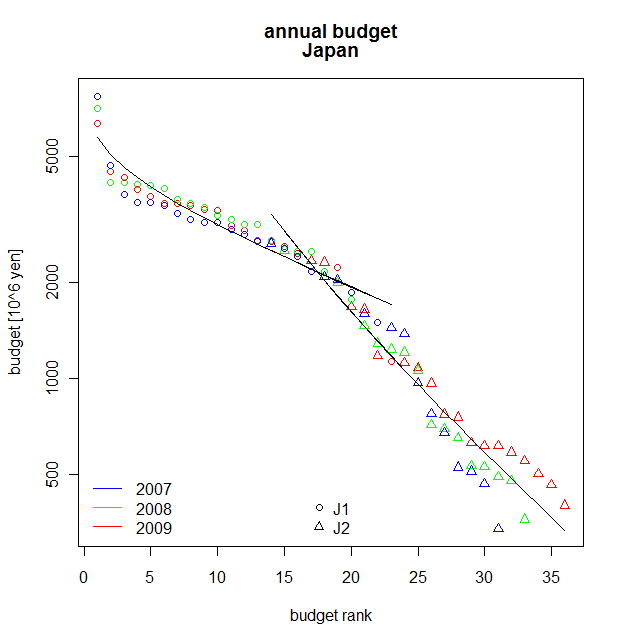
\includegraphics{fig/japan-budget.png}
		\end{center}
		\caption{Jリーグの営業支出}\label{fig:Jリーグの営業支出}
	\end{figure} %}
%s1:Jリーグの営業支出}

\section{スペインリーグの予算}\label{s1:スペインリーグの予算} %{
	Webでサッカーのスペインリーグでの予算(表\ref{tab:スペインリーグでの予算})
	が掲載されていたので、予算の分布と予算と成績との関係を調べてみた。
	\begin{equation*}\begin{array}{rcrcrl} %{
		\ln(\text{予算額}) &=& 6.2884 &-& 1.0953 & \ln(\text{予算順位}) \\
		\ln(\text{予算額}) &=& 5.9715 &-& 0.9397 & \ln(\text{リーグ戦順位}) \\
		\text{得点} &=& -14.223 &+& 8.996 & \ln(\text{予算額}) \\
		\ln(\text{失点}) &=& 4.00974 &-& 0.24946\ & \ln(\text{予算額}) \\
	\end{array}\end{equation*} %}
	予算額の値はちょっと嘘くさいと思う。このデータからほぼ
	\begin{equation*}\begin{split} %{
		\text{チームの予算額}
			=\frac{\text{予算順位一位の予算額}}{\text{チームの予算順位}}
	\end{split}\end{equation*} %}
	という関係が成り立つことになるが、あまりにもデータの値が揃いすぎている。
	普通に考えるともっとデータの値にばらつきがあると思う。

\begin{table}[!htbp]
\begin{center}
\begin{tabular}{rlrrrr} \hline
& チーム & 予算 [$10^6$ euro] & リーグ戦順位 & 得点 & 失点 \\ \hline
1 & Barcelona & 428.00 &   1 &  51 &   9 \\ 
2 & RealMadrid & 442.00 &   2 &  39 &  12 \\ 
3 & Villareal & 67.00 &   3 &  30 &  14 \\ 
4 & Valencia & 131.00 &   4 &  24 &  19 \\ 
5 & Espanol & 50.00 &   5 &  18 &  22 \\ 
6 & AtleticoMadrid & 110.00 &   6 &  27 &  19 \\ 
7 & Getafe & 24.00 &   7 &  27 &  19 \\ 
8 & AthleticBilbao & 53.10 &   8 &  25 &  27 \\ 
9 & RealSociedad & 35.00 &   9 &  22 &  26 \\ 
10 & Mallorca & 36.00 &  10 &  16 &  20 \\ 
11 & Sevilla & 90.00 &  11 &  21 &  27 \\ 
12 & Hercules & 42.00 &  12 &  18 &  22 \\ 
13 & Deportivo & 65.00 &  13 &  13 &  19 \\ 
14 & Racing & 42.00 &  14 &  13 &  23 \\ 
15 & Osasuna & 28.90 &  15 &  15 &  20 \\ 
16 & Levante & 20.00 &  16 &  18 &  26 \\ 
17 & Almeria & 28.00 &  17 &  15 &  25 \\
18 & Malaga &  &  18 &  20 &  35 \\ 
19 & Sporting & 25.00 &  19 &  12 &  23 \\ 
20 & Zaragoza & 24.50 &  20 &  13 &  26 \\ \hline
\end{tabular}
\caption{スペインリーグでの予算(2010-2011)と成績(2010/12/28)}
\label{tab:スペインリーグでの予算}
\end{center}
\end{table}

\begin{lstlisting}[caption=予算額と予算順位, label=code:予算額と予算順位]
Call:
lm(formula = log(budget) ~ log(rank))

Residuals:
     Min       1Q   Median       3Q      Max 
-0.20988 -0.05314 -0.02577  0.02378  0.52995 

Coefficients:
            Estimate Std. Error t value Pr(>|t|)    
(Intercept)   6.2884     0.1003   62.68  < 2e-16 ***
log(rank)    -1.0953     0.0453  -24.18 1.32e-14 ***
---
Signif. codes:  0 ‘***’ 0.001 ‘**’ 0.01 ‘*’ 0.05 ‘.’ 0.1 ‘ ’ 1 

Residual standard error: 0.1552 on 17 degrees of freedom
Multiple R-squared: 0.9717,     Adjusted R-squared: 0.9701 
F-statistic: 584.6 on 1 and 17 DF,  p-value: 1.320e-14
\end{lstlisting}

\begin{lstlisting}[caption=予算額とリーグ戦順位, label=code:予算額とリーグ戦順位]
Call:
lm(formula = log(budget) ~ log(rank))

Residuals:
     Min       1Q   Median       3Q      Max 
-0.96483 -0.28777  0.02317  0.22630  0.78168 

Coefficients:
            Estimate Std. Error t value Pr(>|t|)    
(Intercept)   5.9715     0.3107   19.22 5.73e-13 ***
log(rank)    -0.9397     0.1398   -6.72 3.59e-06 ***
---
Signif. codes:  0 ‘***’ 0.001 ‘**’ 0.01 ‘*’ 0.05 ‘.’ 0.1 ‘ ’ 1 

Residual standard error: 0.4828 on 17 degrees of freedom
Multiple R-squared: 0.7265,     Adjusted R-squared: 0.7104 
F-statistic: 45.16 on 1 and 17 DF,  p-value: 3.59e-06 
\end{lstlisting}

\begin{lstlisting}[caption=予算額と得点, label=code:予算額と得点]
Call:
lm(formula = goal.plus ~ log(budget))

Residuals:
    Min      1Q  Median      3Q     Max 
-10.331  -2.853  -1.402   3.863  12.632 

Coefficients:
            Estimate Std. Error t value Pr(>|t|)    
(Intercept)  -14.223      6.477  -2.196   0.0423 *  
log(budget)    8.996      1.574   5.715 2.53e-05 ***
---
Signif. codes:  0 ‘***’ 0.001 ‘**’ 0.01 ‘*’ 0.05 ‘.’ 0.1 ‘ ’ 1 

Residual standard error: 5.992 on 17 degrees of freedom
Multiple R-squared: 0.6577,     Adjusted R-squared: 0.6375 
F-statistic: 32.66 on 1 and 17 DF,  p-value: 2.528e-05
\end{lstlisting}

\begin{lstlisting}[caption=予算額と失点, label=code:予算額と失点]
Call:
lm(formula = log(goal.minus) ~ log(budget))

Residuals:
     Min       1Q   Median       3Q      Max 
-0.32176 -0.09565  0.01372  0.08273  0.40864 

Coefficients:
            Estimate Std. Error t value Pr(>|t|)    
(Intercept)  4.00974    0.20741  19.332 5.21e-13 ***
log(budget) -0.24946    0.05041  -4.948 0.000122 ***
---
Signif. codes:  0 ‘***’ 0.001 ‘**’ 0.01 ‘*’ 0.05 ‘.’ 0.1 ‘ ’ 1 

Residual standard error: 0.1919 on 17 degrees of freedom
Multiple R-squared: 0.5902,     Adjusted R-squared: 0.5661 
F-statistic: 24.49 on 1 and 17 DF,  p-value: 0.0001221 
\end{lstlisting}

%s1:スペインリーグの予算}

%\section{使う記号}\label{s1:使う記号} %{
	よく使う記号を列挙しておく。
	\begin{description}\setlength{\itemsep}{-1mm} %{
		\item[自然数]
		$0$以上の自然数を自然数を$\sizen$、$1$以上の自然数を$\sizen_+$と書く。
		$i$以上$j$以下の自然数の集合を$i..j$と書く。$i..j$と書いて$j<i$の場合
		は空集合とする。
		\item[よく使う集合]
		元が一つもない集合を$\mybf{0}$、元が一つだけの集合を$\mybf{1}$と書く。
		整数を$\sei$、実数を$\jitu$、複素数を$\fukuso$と書く。
		\item[ブーリアン]
		ブーリアンを$\bool=\set{0,1}$と書く。ブーリアンの論理和を$\mybiop{+}$、
		論理積を$\mybiop{\myspace}$と書く。
		\item[冪集合]
		集合$A$に対して、空集合も含む$A$の冪集合を$PA$、空集合を含まない
		$A$の冪集合を$P_+A$と書く。
		\item[文字列集合]
		集合$A$に対して、$A$の元を文字とする長さ$0$以上の文字列の集合を$WA$、
		長さ$1$以上の文字列の集合を$W_+A$と書く。
		\item[半モジュール]
		集合$A$、半環$R$に対して、$A$を基底とする$R$係数自由半モジュールを
		$RA$と書く。
		\item[写像]
		集合$A,B$に対して、$A$から$B$への写像全体のつくる空間を$\set{A\to B}$
		や$\myop{map}(A,B)$と書く。
		\item[デルタ関数]
		論理式を$\jump{}$で囲ってデルタ関数を表す。
		\begin{equation*}\begin{split} %{
			\jump{\text{expression}} &= \begin{cases}
				1, &\text{ iff }\text{expression is true} \\
				0, &\text{ otherwise } \\
			\end{cases}
		\end{split}\end{equation*} %}
	\end{description} %}

\subsection{文字列集合}\label{s2:文字列集合} %{
	$A$を集合、$WA$を$A$の元を文字とする文字列の集合とする。
	\begin{itemize}\setlength{\itemsep}{-1mm} %{
		\item 長さ$0$の文字列、つまり空の単語を$1_W$と書く。
		\item 文字列は通常の直積の元の書き方$(a_1,a_2,\dots,a_m)$の他に
		$\bakko{a_1a_2\cdots a_m}$というように文字を並べてカギ括弧で囲って
		表すこともある。
		\item 文字列$w_1$と$w_2$の連結(juxtaposition)を$w_1*w_2$と書く。
		例えば、$[abc]*[de]=[abcde]$となる。
		\item 文字列$w$に含まれる文字$a$の数を$\sharp_aw$と書く。
		例えば、$\sharp_a[abcba]=2$となる。
	\end{itemize} %}

	$R$を半環、$RWA$を$WA$を基底とする$R$係数自由半モジュールとする。
	余積$\Delta_*$を次のように定義する。
	\begin{equation}\label{eq:連結余積の定義}\begin{array}{rcll} %{
		\Delta_*1_W &=& 1_W\otimes1_W \\
		\Delta_*[a] &=& [a]\otimes1_W+1_W\otimes[a] & \text{for all }a\in A \\
		\Delta_*(w_1*w_2*\cdots*w_m) &=& (\Delta_*w_1)*(\Delta_*w_2)*\cdots
			*(\Delta_*w_m) & \text{for all }w_1,w_2,\dots,w_m\in WA
	\end{array}\end{equation} %}
	ここで、テンソル積に対する積を
	$(w_1\otimes w_2)*(w_3\otimes w_4)=(w_1*w_3)\otimes(w_2*w_4)$とした。
	定義より余積$\Delta_*$と積$\mybiop{*}$は互いに準同型となっている。
	この余積$\Delta_*$を連結余積と書くことにする。

	\begin{definition}[連結余積]\label{def:連結余積} %{
		式\eqref{eq:連結余積の定義}で定義された余積$\Delta_*$を連結余積
		ということにする。
	\end{definition} %def:連結余積}
%s2:文字列集合}
%s1:使う記号}

\section{球を箱に入れる仕方の数}\label{s1:球を箱に入れる仕方の数} %{
	球を箱に入れる仕方の数を次のバリエーションで考えてみる。
	考え方は文献\cite{html:iga.math}に従う。
	\begin{itemize}\setlength{\itemsep}{-1mm} %{
		\item 球が区別つく場合とつかない場合
		\item 箱が区別つく場合とつかない場合
		\item 空の箱を許すか許さないか
	\end{itemize} %}
	次のパターンを使って、空の箱を許す場合と許さない場合のどちらか簡単な
	方で球を箱に入れる仕方の数を計算して他方を導くことが多い。
	\begin{equation}\label{eq:空箱ありは空箱なしの直和}\begin{split} %{
		k\text{箱に空箱を許して入れる仕方} 
		&= 1\text{箱に空箱を許さず入れる仕方} \\
		&+ 2\text{箱に空箱を許さず入れる仕方} \\
		&+ \cdots \\
		&+ k\text{箱に空箱を許さず入れる仕方}
	\end{split}\end{equation} %}
\subsection{球と箱が区別つく場合}\label{s2:球と箱が区別つく場合} %{
\subsubsection{空箱を許す場合}\label{s3:空箱を許す場合} %{
	球$1$を箱$a_1$に入れ、球$2$を箱$a_2$に入れ、、、球$n$を箱$a_n$に入れた
	状態を文字列$[a_1a_2\cdots a_m]$で表す。すると、$n$個の球を$k$個の箱へ
	入れる仕方は、$1..n$を文字とする長さ$n$の文字列で表すことができることが
	わかる。したがって、$n$個の球を$k$個の箱へ入れた状態空間は$(1..k)^n$
	になることがわかる。また、入れ方の仕方の数は$k^n$になることもわかる。
%s3:空箱を許す場合}
\subsubsection{空箱を許さない場合}\label{s3:空箱を許さない場合} %{
	$n$個の球を$k$個の箱に入れる仕方は、文字列集合$(1..k)^n$を、
	文字列の中に$1..k$のすべての文字が含まれるものに制限したものになる。
	これを$\mycal{A}_k^n$と書く。
	\begin{equation*}\begin{split} %{
		\mycal{A}_k^n &= \set{w\in (1..k)^n
			\bou 1\le \sharp_aw \quad\text{for all }a\in (1..k)}
	\end{split}\end{equation*} %}
	$n<k$の場合は、空の箱を許さない入れ方は不可能なので、$\mycal{A}_k^n$
	は空集合と定義する。

	$\mycal{A}_k^n$は集合として由緒正しいものである。集合同型の意味で
	次の式が成り立つ。
	\begin{equation*}\begin{split} %{
		(1..k)^n &\simeq \set{1..n\to 1..k} \\
		\mycal{A}_k^n &\simeq \set{f:1..n\to 1..k\bou f\text{は}\myop{onto}} \\
	\end{split}\end{equation*} %}

	$\mycal{A}_k^n$の大きさを調べる。まず、簡単な例から始める。
	$\mycal{A}_2^3$は次のようになり、
	\begin{equation*}\begin{split} %{
		(1..2)^3 &= \set{[111],[112],[121],[122],[211],[212],[221],[222]} \\
		\mycal{A}_2^3 &\simeq \set{[112],[121],[122],[211],[212],[221]} \\
		\mycal{A}_1^3 &\simeq \set{[111]} \\
		\mycal{A}_1^3 &\simeq \set{[222]} \\
	\end{split}\end{equation*} %}
	$\zettai{(1..2)^3}=\zettai{\mycal{A}_2^3}+2\zettai{\mycal{A}_1^3}$と
	書けることがわかる。\footnote{
		半モジュールで$\sizen(1..2)^3\simeq
		\sizen\mycal{A}_2^3\oplus\sizen\mycal{A}_1^3\oplus\sizen\mycal{A}_1^3$
		と書いた方がわかり易いかもしれない。
	}

	この関係の一般の場合がパターン\eqref{eq:空箱ありは空箱なしの直和}である。
	ただし、空でない$p$個の箱を選びだす仕方は$\binom{k}{p}$通りある。
	したがって、$A_k^n=\zettai{\mycal{A}_k^n}$と書くと、任意の
	$k,n\in\sizen_+$に対して次の漸化式が成り立つ。
	\begin{equation}\label{eq:空箱ありの仕方の数は空箱なし仕方の数の和}\begin{split} %{
		k^n = \sum_{p\in1..k}\binom{k}{p}A_p^n
	\end{split}\end{equation} %}
	ただし、$n<k$の場合は$A_k^n=0$である。この漸化式を行列の形で書くと
	$K = CA$となる。ここで、$K,C,B$はそれぞれ次のように定義した。
	\begin{equation*}\begin{split} %{
		K = \begin{pmatrix}
			k^n \\ (k-1)^n \\ \vdots \\ 1^n
		\end{pmatrix} 
		,\quad B = \begin{pmatrix}
			A_k^n \\ A_{k-1}^n \\ \vdots \\ A_1^n
		\end{pmatrix}
		,\quad C = \begin{pmatrix}
			\binom{k}{0} & \binom{k}{1} & \cdots & \binom{k}{k-1} \\
			0 & \binom{k-1}{0} & \cdots & \binom{k-1}{k-2} \\
			\vdots & \vdots & \cdots & \vdots \\
			0 & 0 & \cdots & \binom{1}{0} \\
		\end{pmatrix} 
	\end{split}\end{equation*} %}
	行列$C$の逆行列が求まれば$C^{-1}K$によって$B$が求まる。
	$C$の行列式は$1$だから逆行列を持ち次のようになる。
	\begin{equation*}\begin{split} %{
		C^{-1} = \begin{pmatrix}
			\binom{k}{0} & -\binom{k}{1} & \cdots & (-)^{k-1}\binom{k}{k-1} \\
			0 & \binom{k-1}{0} & \cdots & (-)^{k-2}\binom{k-1}{k-2} \\
			\vdots & \vdots & \cdots & \vdots \\
			0 & 0 & \cdots & \binom{1}{0} \\
		\end{pmatrix}
	\end{split}\end{equation*} %}
	したがって漸化式が解けて、任意の$k,n\in\sizen_+$に対して次のようになる。
	\begin{equation}\label{eq:分配の大きさ}\begin{split} %{
		A_k^n &= \begin{cases}
			\alpha_k^n, &\text{ iff }k\le n \\
			0, &\text{ otherwise } \\
		\end{cases} \\
		\alpha_k^n &= \sum_{p\in1..k}(-)^{k-p}\binom{k}{p}p^n
	\end{split}\end{equation} %}
%s3:空箱を許さない場合}
%s2:球と箱が区別つく場合}
\subsection{球が区別つき、箱が区別つかない場合}\label{s2:球が区別つき、箱が区別つかない場合} %{
\subsubsection{空箱を許す場合}\label{s3:空箱を許す場合} %{
	球と箱が区別つかない場合の仕方$(1..k)^n$を箱の並び順を対称化すれば、
	この場合の仕方が得られる。式で書くと、$S_k$を$k$次対称群として、
	同値関係$\sim_\sqcup$を次のように定義し、
	\begin{equation*}\begin{split} %{
		[a_1a_2\cdots a_n]
		\sim_\sqcup [(\sigma a_1)(\sigma a_2)\cdots(\sigma a_n)]
		\quad\text{for all }\sigma\in S_k
	\end{split}\end{equation*} %}
	商集合$(1..k)^n/\sim_\sqcup$がこの場合の仕方となる。

	$(1..k)^n/\sim_{\sqcup}$の大きさは、単純に$(1..k)^n$の大きさを$S_k$の
	大きさで割ったものにならない。一般には次のようになる。
	\begin{equation*}\begin{split} %{
		\frac{\zettai{(1..k)^n}}{\zettai{S_k}} 
		= \frac{k^n}{k!}\le \zettai{(1..k)^n/\sim_{\sqcup}}
	\end{split}\end{equation*} %}
	$(1..3)^3$の例で説明する。球$1$が箱$1$に、球$2$が箱$2$に、球$3$が箱$1$
	に入った状態を$\bakko{\set{13}\set{2}\set{}}$と書くことにする。
	この記法を使うと、$\bakko{\set{1}\set{2}\set{3}}$の$\sim_\sqcup$同値類
	は次の$6$個なのに対し、
	\begin{equation*}\begin{array}{ccc} %{
		\bakko{\set{1}\set{2}\set{3}} & \bakko{\set{1}\set{3}\set{2}} 
			& \bakko{\set{2}\set{1}\set{3}} \\
		\bakko{\set{2}\set{3}\set{1}} & \bakko{\set{3}\set{1}\set{2}} 
			& \bakko{\set{3}\set{2}\set{1}}
	\end{array}\end{equation*} %}
	$\bakko{\set{123}\set{}\set{}}$の$\sim_\sqcup$同値類は次の$3$個
	しかない。
	\begin{equation*}\begin{array}{ccc} %{
		\bakko{\set{123}\set{}\set{}} & \bakko{\set{}\set{123}\set{}}
			& \bakko{\set{}\set{}\set{123}}
	\end{array}\end{equation*} %}
	この例は空箱同士を入れ替えても$(1..k)^n$の状態が変わらない例になって
	いる。箱を入れ替える操作で不変になっている$(1..k)^n$の元があるために、
	単純に$k^n/k!$が$(1..k)^n/\sim_\sqcup$の大きさにならない理由である。

	$(1..k)^n/\sim_\sqcup$の大きさを直接計算することが難しいので、
	空箱を許さない場合に球を箱に入れる仕方の数が計算できることを祈りつつ、
	パターン\eqref{eq:空箱ありは空箱なしの直和}を使うと、次のようになる。
	\begin{equation*}\begin{split} %{
		\zettai{(1..k)^n/\sim_\sqcup}
		= \sum_{p=1..k}
		\text{空箱を許さずに$n$個の球を$k$個の箱に入れる仕方の数}
	\end{split}\end{equation*} %}
%s3:空箱を許す場合}
\subsubsection{空箱を許さない場合}\label{s3:空箱を許さない場合} %{
	空箱を許す場合\ref{s3:空箱を許す場合}と同様に、箱が区別つく場合の
	仕方$\mycal{A}_k^n$を箱について対称化すれば、この場合の仕方
	$\mycal{B}_k^n=\mycal{A}_k^n/\sim_\sqcup$が得られる。
	定義より$\mycal{A}_k^n$に箱を入れ替える操作で不変な状態はない。
	\begin{equation}\label{eq:空箱を許さない場合の効果的な箱変換}\begin{split} %{
		[(\sigma a_1)(\sigma a_2)\cdots(\sigma a_n)] = [a_1a_2\cdots a_n]
			\implies \sigma = \myid \\
		\quad\text{for all }[a_1a_2\cdots a_n]\in\mycal{A}_k^n
			,\;\sigma\in S_k
	\end{split}\end{equation} %}
	したがって、$\mycal{B}_k^n$の大きさは、単純に$\mycal{A}_k^n$の大きさを
	$S_k$の大きさで割ったものになる。
	\begin{equation}\label{eq:第二種スターリング数}\begin{split} %{
		\zettai{\mycal{B}_k^n} = \begin{cases}
			\frac{1}{k!}A_k^n, &\text{ iff }k\le n \\
			0, &\text{ otherwise } \\
		\end{cases} \quad\text{for all }k,n\in \mybf{N}
	\end{split}\end{equation} %}
	空の箱を許さない場合は、空の箱を許す場合と異なり、箱が区別つく場合の
	状態空間に箱の変換群が効果的に作用している
	(式\eqref{eq:空箱を許さない場合の効果的な箱変換})
	ことが大きさの計算が容易になっているミソである。

	ここで求めた集合の大きさ$\zettai{\mycal{B}_k^n}$のことを第二種
	スターリング数という。

	\begin{definition}[第二種スターリング数(Stirling number of 2nd kind)]\label{def:第二種スターリング数} %{
		式\eqref{eq:第二種スターリング数}の$\zettai{\mycal{B}_k^n}$を
		第二種スターリング数という。
	\end{definition} %def:第二種スターリング数}
%s3:空箱を許さない場合}
%s2:球が区別つき、箱が区別つかない場合}
\subsection{球の区別がつかず、箱の区別がつく場合}\label{s2:球の区別がつかず、箱の区別がつく場合} %{
\subsubsection{空箱を許す場合}\label{s3:空箱を許す場合} %{
	この場合の球を箱に入れる仕方の数は巧妙な方法で求められる。
	\begin{itemize}\setlength{\itemsep}{-1mm} %{
		\item $k$個の箱に一つづつ球を入れた状態でスタートする。
		\item $n$個の球を箱に分配する。
		\item すると、$k$個すべての箱が空でなく、$n$個の球を箱に仕方の数と
		同数の状態が出現する。
	\end{itemize} %}
	したがって、$n$個の球を$k$個の箱に空箱を許して入れる仕方の数は、
	$n+k$個の球を$k$個の箱に空箱を許さず入れる仕方の数になる。
%s3:空箱を許す場合}
\subsubsection{空箱を許さない場合}\label{s3:空箱を許さない場合} %{
	この場合の球を箱へ入れる仕方$\mycal{C}_k^n$は、$n=a_1+a_2+\cdots+a_k$
	となる$\sizen_+$を文字とする長さ$k$の文字列$[a_1a_2\cdots a_k]$全体
	の作る集合となる。式で書くと次のようになる。
	\begin{equation*}\begin{split} %{
		\mycal{C}_k^n = \set{[a_1a_2\cdots a_k]\in \mybf{N}_+^k
			\bou a_1+a_2+\cdots+a_k=n}
	\end{split}\end{equation*} %}
	$\mycal{C}_k^n$の大きさは次のようにして求めることができる。
	\begin{itemize}\setlength{\itemsep}{-1mm} %{
		\item $1$の間に$\square$を挟んで次のように書く。
		\begin{equation*}\begin{split} %{
			\underbrace{1\square 1\square \cdots \square 1}
				_{1\text{が}n\text{個}}
		\end{split}\end{equation*} %}
		\item $\square$に$+$または$\myspace$を書き込むと$\mycal{C}_k^n$
		の元となる。
	\end{itemize} %}
	例えば$n=3$であれば次のようになる。
	\begin{equation*}\begin{array}{rclclcl} %{
		1\square 1\square 1
		&\xrightarrow{(++)}& 1+1+1 &=& 3 &\in& \mycal{C}_1^3 \\
		&\xrightarrow{(+,\myspace)}& 1+1\myspace 1 &=& 2\myspace 1 
			&\in& \mycal{C}_2^3 \\
		&\xrightarrow{(\myspace,+)}& 1\myspace 1+1 &=& 1\myspace 2 
			&\in& \mycal{C}_2^3 \\
		&\xrightarrow{(\myspace,\myspace)}& 1\myspace 1\myspace 1
			&=& 1\myspace 1\myspace 1 &\in& \mycal{C}_3^3 \\
	\end{array}\end{equation*} %}
	一般の$\mycal{C}_k^n$では、$n-1$個の$\square$の中から$k-1$個を選択
	して、そこに$\myspace$を書き込むと$\mycal{C}_k^n$の状態ができる。
	したがって、$\mycal{C}_k^n$の大きさは次のようになることがわかる。
	\begin{equation*}\begin{split} %{
		\zettai{\mycal{C}_k^n} = \begin{cases}
			\binom{n-1}{k-1}, &\text{ iff } k\le n \\
			0, &\text{ otherwise } \\
		\end{cases} \quad\text{for all }k,n\in \mybf{N}_+
	\end{split}\end{equation*} %}
	また、この構成方法より、$\sum_{k\in(1..n)}\mycal{C}_k^n$は、
	集合$\set{+,\myspace}$を文字とする長さ$n-1$の文字列全体と集合同型となる
	ことがわかり、次の式が導かれる。
	\begin{equation*}\begin{split} %{
		2^{n-1} = \sum_{k\in(1..n)}\binom{n-1}{k-1}
	\end{split}\end{equation*} %}

	$\mycal{C}_k^n$の状態を$n$の合成という。

	\begin{definition}[自然数の合成(Composition)]\label{def:自然数の合成(Composition)} %{
		$\mycal{C}_k^n$の元を長さ$n$の$k$の合成という。
	\end{definition} %def:自然数の合成(Composition)}
%s3:空箱を許さない場合}
%s2:球の区別がつかず、箱の区別がつく場合}
\subsection{まとめ}\label{s2:まとめ} %{
	$n$個の球を$k$個の箱に分配する仕方を次のバリエーションごとに調べた。
	\begin{itemize}\setlength{\itemsep}{-1mm} %{
		\item 球が区別つく場合とつかない場合
		\item 箱が区別つく場合とつかない場合
		\item 空の箱を許すか許さないか
	\end{itemize} %}
	それらをまとめると、$n$個の球を$k$個の箱に入れる仕方の数は次のように
	なる。
	\begingroup
	\renewcommand{\arraystretch}{1.5}
	\begin{equation}\label{eq:球を箱に入れる仕方の数の表}\begin{array}{cccc} %{
		\text{球の区別} & \text{箱の区別} & \text{空箱} & \text{仕方の数} \\
		\text{有り} & \text{有り} & \text{有り} & k^n \\
		\text{有り} & \text{有り} & \text{無し} & k!B_k^n \\
		\text{有り} & \text{無し} & \text{有り} & \sum_{k\in1..n}B_k^n \\
		\text{有り} & \text{無し} & \text{無し} & B_k^n \\
		\text{無し} & \text{有り} & \text{有り} & \binom{n+k-1}{k-1} \\
		\text{無し} & \text{有り} & \text{無し} & C_k^n \\
	\end{array}\end{equation} %}
	\endgroup
	ここで、$B_k^n$と$C_k^n$はそれぞれ次のように定義される。
	\begin{equation*}\begin{split} %{
		B_k^n &= \begin{cases}
			\frac{1}{k!}\sum_{p\in(1..k)}(-)^{k-p}\binom{k}{p}p^n, &\text{ iff }k\le n \\
			0, &\text{ otherwise } \\
		\end{cases} \\
		C_k^n &= \begin{cases}
			\binom{n-1}{k-1}, &\text{ iff }k\le n \\
			0, &\text{ otherwise } \\
		\end{cases} \\
	\end{split}\end{equation*} %}
%s2:まとめ}
%s1:球を箱に入れる仕方の数}

\section{球を箱に空箱を許さず入れる仕方}\label{s1:球を箱に空箱を許さず入れる仕方} %{
	前節に引き続き、球を箱に空箱を許さず入れる仕方を考える。この節では
	球も箱も区別できない場合も考える。$n$個の球を$k$個の箱に入れる仕方を
	次のように定義する。
	\begin{itemize}\setlength{\itemsep}{-1mm} %{
		\item 球と箱も区別つく場合を$\mycal{A}_k^n$とする。
		\item 球が区別つき、箱が区別つかない場合を$\mycal{B}_k^n$とする。
		\item 球が区別つかず、箱が区別つく場合を$\mycal{C}_k^n$とする。
		\item 球と箱も区別つかない場合を$\mycal{P}_k^n$とする。
	\end{itemize} %}
	箱を対称化する操作を$\pi_\sqcup$、球を対称化する操作を$\pi_\circ$
	と書く。それぞれの集合は次の$\myop{onto}$写像の可換図によっても表される。
	\begin{equation*}\xymatrix@C=6pc{
		\mycal{A}_k^n \ar[r]_{\text{球を対称化}}^{\pi_\circ}
		 \ar[d]_{\text{箱を対称化}}^{\pi_\sqcup}
			& \mycal{C}_k^n \ar[d]_{\text{箱を対称化}}^{\pi_\sqcup} \\
		\mycal{B}_k^n \ar[r]_{\text{球を対称化}}^{\pi_\circ} & \mycal{P}_k^n \\
	}\end{equation*}
	前節の結果をもう一度書くと、$n$個の球を$k$個の箱に入れる仕方の数は
	次のようになる。
	\begingroup
	\renewcommand{\arraystretch}{1.5}
	\begin{equation*}\begin{array}{cccc} %{
		\text{球の区別} & \text{箱の区別} & \text{集合} & \text{集合の大きさ} \\
		\text{有り} & \text{有り} & \mycal{A}_k^n & k!B_k^n \\
		\text{有り} & \text{無し} & \mycal{B}_k^n & B_k^n \\
		\text{無し} & \text{有り} & \mycal{C}_k^n & C_k^n \\
		\text{無し} & \text{無し} & \mycal{P}_k^n & \text{不明} \\
	\end{array}\end{equation*} %}
	\endgroup
	\begin{equation*}\begin{split} %{
		B_k^n &= \begin{cases}
			\frac{1}{k!}\sum_{p\in(1..k)}(-)^{k-p}\binom{k}{p}p^n, 
				&\text{ iff }k\le n \\
			0, &\text{ otherwise } \\
		\end{cases} \\
		C_k^n &= \begin{cases}
			\binom{n-1}{k-1}, &\text{ iff }k\le n \\
			0, &\text{ otherwise } \\
		\end{cases} \\
	\end{split}\end{equation*} %}
	$\mycal{P}_k^n$は$n$の$k$分割といい、その大きさを表す簡単な式はない
	ようだ。

	$\mycal{X}\in\set{\mycal{A},\mycal{B},\mycal{C},\mycal{P}}$として、
	次のように拡張して添え字$k,n$を自然数$\sizen$にとれるようにしておく。
	\begin{itemize}\setlength{\itemsep}{-1mm} %{
		\item $\mycal{X}_0^0=\set{\bullet}$とする。
		\item 任意の$n\in\sizen_+$に対して$\mycal{X}_0^n=\emptyset$とする。
		\item 任意の$k\in\sizen_+$に対して$\mycal{X}_k^0=\emptyset$とする。
		\item 任意の$k<n\in\sizen$に対して$\mycal{X}_k^n=\emptyset$とする。
	\end{itemize} %}
	記号$\bullet$は箱も球もない状態を表す。
	また、
	\begin{itemize}\setlength{\itemsep}{-1mm} %{
		\item $\mycal{X}_*^n=\sum_{k\in0..n}\mycal{X}_k^n$、
		\item $\mycal{X}_*^*=\sum_{n\in\sizen}\mycal{X}_*^n$
	\end{itemize} %}
	と書くことにする。

	$\mycal{A}_k^n$の元を$WW_+(1..k)$の部分集合として$2$次元の文字列で
	次のように書き表すことにする。
	\begin{equation*}\begin{split} %{
		\bigl[[1][4][23]\bigr] = \bigl((1),(4),(2,3)\bigr) 
		= \left\{\begin{array}{l}
			\text{箱$1$に球$1$} \\
			\text{箱$2$に球$4$} \\
			\text{箱$3$に球$2$と球$3$} \\
			\end{array}\right\}\text{入った状態}
	\end{split}\end{equation*} %}
	$\mycal{B}_k^n$の元を$WW_+(1..k)$の部分集合として$2$次元の文字列で
	表す場合は、箱に入っている球の最も小さい数字によって、箱を左から右へ順に
	並べるものとする。例えば次のようになる。
	\begin{equation*}\begin{split} %{
		\bigl[[1][4][23]\bigr]\in\mycal{A}_3^4 
			\xmapsto{\pi_\circ} \bigl[[1][23][4]\bigr]\in\mycal{B}_3^4
	\end{split}\end{equation*} %}
	同様に、$\mycal{C}_k^n$の元を$W(1..n)$の部分集合として文字列で
	次のように書き表すことにする。
	\begin{equation*}\begin{split} %{
		[121] = (1,2,1) = \left\{\begin{array}{l}
			\text{箱$1$に球が$1$個} \\
			\text{箱$2$に球が$2$個} \\
			\text{箱$3$に球が$1$個} \\
			\end{array}\right\}\text{入った状態}
	\end{split}\end{equation*} %}
	$\mycal{P}_k^n$の元を$W(1..n)$の部分集合として文字列で表す場合は、
	箱に入っている球の数が右から左に小さくなるように並べるとする。例えば
	次のようになる。
	\begin{equation*}\begin{split} %{
		[121]\in\mycal{C}_3^4 
			\xmapsto{\pi_\sqcup} [211]\in\mycal{P}_3^4
	\end{split}\end{equation*} %}

	集合$\mycal{B}_k^n$と$\mycal{P}_k^n$の元を図形で表す方法を定義しておく。

	\begin{definition}[ヤング図形]\label{def:ヤング図形} %{
		任意の$n\in\mybf{N}_+$に対して次の条件を満たす二次元配列を
		$n$次のヤング図形という。
		\begin{itemize}\setlength{\itemsep}{-1mm} %{
			\item 各行の長さが一定とは限らない。
			\item 空の行を含まない。
			\item 升目の総数が$n$である。
			\item 各行の長さは上から下へ同じか減少していく。
		\end{itemize} %}
	\end{definition} %def:ヤング図形}

	ヤング図形は歴史も長くいろいろな場面で使われるために、次のような
	慣用的な書き方がある。
	\begin{itemize}\setlength{\itemsep}{-1mm} %{
		\item ヤング図形は記号$\lambda$で書かれる。
		\item ヤング図形$\lambda\vdash n$は$n$次のヤング図形を表す。
		\item ヤング図形$\lambda=[\lambda_1\lambda_2\cdots\lambda_k]$
		とは、$1$行目の長さが$\lambda_1$、$2$行目の長さが$\lambda_2$、、、$k$
		行目の長さが$\lambda_k$という$k$行のヤング図形を表すものとする。
		\item 分割$n=\lambda_1+\lambda_2+\dots+\lambda_k$のヤング図形とは、
		$1$行目の長さが$\lambda_1$、$2$行目の長さが$\lambda_2$、、、$k$行目の
		長さが$\lambda_k$という$k$行のヤング図形を表すものとする。
	\end{itemize} %}

	\begin{definition}[分配盤]\label{def:分配盤} %{
		任意の$n\in\mybf{N}_+$に対して次の条件を満たす二次元配列を
		$n$次の分配盤と言うことにする。
		\begin{itemize}\setlength{\itemsep}{-1mm} %{
			\item 各行の長さが一定とは限らない。
			\item 空の行を含まない。
			\item 升目の総数が$n$である。
			\item 升目には$1$から$n$までの数字が重複無く書かれている。
			\item 一列目の数字は上から下へ増加していく。
			\item 各行で数字は左から右へ増加していく。
		\end{itemize} %}
	\end{definition} %def:分配盤}

	ヤング図形の行のことを箱ともいう。分配盤の行のことを箱、升目の中に
	書かれている数字ことを球のラベルともいう。
	$n$次$k$行のヤング図形全体の作る集合が$\mycal{P}_k^n$となり、
	$n$次$k$行の分配盤全体の作る集合が$\mycal{B}_k^n$となる。

	以下の節では、順不同で球を箱に入れる仕方に関連する話題を書くことにする。
	
\subsection{対称化の逆の大きさ}\label{s2:対称化の逆の大きさ} %{
	対称化$\pi_\sqcup$と$\pi_\circ$の逆写像の大きさをそれぞれの
	次のようになる。
	\begin{itemize}\setlength{\itemsep}{-1mm} %{
		\item $\pi_\sqcup:\mycal{A}_k^n\to\mycal{B}_k^n$の場合、
		逆写像の大きさは次のようになる。
		\begin{equation*}\begin{split} %{
			\zettai{\pi_\circ^{-1}t} = k! \quad\text{for all }t\in\mycal{B}_k^n
		\end{split}\end{equation*} %}
		例えば次のようになる。
		\begin{equation*}\begin{split} %{
			\pi_\circ^{-1}\young(12,3) = \Set{\bigl[[12][3]\bigr]
				,\; \bigl[[3][12]\bigr]}
		\end{split}\end{equation*} %}
		\item $\pi_\circ:\mycal{A}_k^n\to\mycal{C}_k^n$の場合、
		逆写像の大きさは次のようになる。
		\begin{equation*}\begin{split} %{
			\zettai{\pi_\circ^{-1}[n_1n_2\cdots n_k]} 
				= \frac{n!}{n_1!n_2!\cdots n_k!}
				\quad\text{for all }[n_1n_2\cdots n_k]\in\mycal{C}_k^n
		\end{split}\end{equation*} %}
		例えば次のようになる。
		\begin{equation*}\begin{split} %{
			\pi_\circ^{-1}[21] = \Set{[12][3]\bigr],\;\bigl[[23][1]\bigr]
				,\;\bigl[[13][2]}
		\end{split}\end{equation*} %}
		\item $\pi_\sqcup:\mycal{B}_k^n\to\mycal{P}_k^n$の場合、
		逆写像の大きさは次のようになる。
		\begin{equation}\label{eq:分配盤とヤング図形の対応数}\begin{split} %{
			\zettai{\pi_\circ^{-1}[\lambda_1\lambda_2\cdots\lambda_k]}
			= \frac{1}{S_\lambda}\frac{n!}{\lambda_1!\lambda_2!\cdots \lambda_k!}
			\quad\text{for all }\lambda
				=[\lambda_1\lambda_2\cdots\lambda_k]\in\mycal{P}_k^n
		\end{split}\end{equation} %}
		ここで、$S_\lambda$はヤング図形$\lambda$の行の重複に対応した数で、
		次のように定義される。
		\begin{equation*}\begin{split} %{
			S:\yng(3,3,2,1,1,1)\mapsto 2!1!3!
		\end{split}\end{equation*} %}
		$\pi_\circ^{-1}$の例は次のようになる。
		\begin{equation*}\begin{split} %{
			\pi_\circ^{-1}\yng(2,1,1) &= \Set{\young(12,3,4),\; \young(1,23,4)
				,\; \young(13,2,4),\; \young(14,2,3),\; \young(1,24,3)
				,\; \young(1,2,34)} \\
			\pi_\circ^{-1}\yng(3,1) &= \Set{\young(123,4),\; \young(124,3)
				,\; \young(134,2),\; \young(1,234)}
		\end{split}\end{equation*} %}
		\item $\pi_\sqcup:\mycal{P}_k^n\to\mycal{C}_k^n$の場合、
		逆写像の大きさは次のようになる。
		\begin{equation*}\begin{split} %{
			\pi_\sqcup^{-1}[\lambda_1\lambda_2\cdots\lambda_k]
			= \frac{k!}{S_\lambda} \quad\text{for all }
				[\lambda_1\lambda_2\cdots\lambda_k]\in\mycal{P}_k^n
		\end{split}\end{equation*} %}
		例えば次のようになる。
		\begin{equation*}\begin{split} %{
			\pi_\sqcup^{-1}\yng(3,2,1) &= \Set{[123],\; [132],\; [213],\; [231]
			,\; [312],\; [321]} \\
			\pi_\sqcup^{-1}\yng(2,1,1) &= \Set{[211],\; [121],\; [112]} \\
			\pi_\sqcup^{-1}\yng(3,1) &= \Set{[31],\; [13]}
		\end{split}\end{equation*} %}
	\end{itemize} %}
	対称化$\pi_\sqcup$と$\pi_\circ$の逆写像の大きさを図(可換図ではない)
	で書くと次のようになる。
	\begin{equation*}\xymatrix@R=4pc@C=8pc{
		\mycal{A}_k^n
			& \mycal{C}_k^n \ar@{|.>}[l]
				^{\frac{n!}{\lambda_1!\lambda_2!\cdots \lambda_k!}}
				_{\pi_\circ^{-1}} \\
		\mycal{B}_k^n \ar@{|.>}[u]^{k!}_{\pi_\sqcup^{-1}} 
			& (\lambda_1,\lambda_2,\dots,\lambda_k)
			\ar@{|.>}[l]^{\frac{1}{S_\lambda}
				\frac{n!}{\lambda_1!\lambda_2!\cdots \lambda_k!}}_{\pi_\circ^{-1}}
			\ar@{|.>}[u]^{\frac{k!}{S_\lambda}}_{\pi_\sqcup^{-1}} \\
	}\end{equation*}
%s2:対称化の逆の大きさ}
\subsection{球を箱に入れる仕方の列挙}\label{s2:球を箱に入れる仕方の列挙} %{
	まず、分配盤に対する自然な成長を定義する。

	\begin{definition}[分配盤の自然な成長]\label{def:分配盤の自然な成長} %{
		分配盤の$k$行目に新しい球を追加する操作を$k$行に対する自然な成長と
		いい、$\myop{grow}_k$と書く。また、$\myop{grow}_0$を新たに行を
		付け足してその行に新しい球を入れる操作とする。
		行に対する自然な成長をベクトル空間$\jitu\mycal{B}_*^*$の
		線形写像に拡張して、次のように定義された線形写像
		$\myop{grow}:\jitu\mycal{B}_*^*\to\jitu\mycal{B}_*^*$を分配盤の
		自然な成長という。
		\begin{equation*}\begin{split} %{
			\myop{grow}t = \sum_{k\in0..k}\myop{grow}_kt
			\quad\text{for all }t\in\mycal{B}_k^n,\;k,n\in\sizen
		\end{split}\end{equation*} %}
	\end{definition} %def:分配盤の自然な成長}

	行に対する自然な成長$\myop{grow}_k,\;1\le k$は任意の$n\in\sizen$の
	$\mycal{B}_0^n,\mycal{B}_1^n,\dots,\mycal{B}_k^n$に対してのみに
	定義され、$\myop{grow}_0$はすべて$\mycal{B}_*^*$に対して定義される。

	\begin{example}[分配盤の自然な成長]\label{eg:分配盤の自然な成長} %{
		行に対する自然な成長は次のようになり、
		\begin{equation*}\begin{split} %{
			\myop{grow}_0\young(1,2) &= \young(1,2,3) \\
			\myop{grow}_1\young(1,2) &= \young(13,2) \\
			\myop{grow}_2\young(1,2) &= \young(1,23) \\
		\end{split}\end{equation*} %}
		自然な成長は次のようになる。
		\begin{equation*}\begin{array}{rrl} %{
			\myop{grow}\young(1,2) &= \young(1,2,3) + \young(13,2) + \young(1,23)
		\end{array}\end{equation*} %}
	\end{example} %eg:分配盤の自然な成長}

	ヤング図形に対しても自然な成長を分配盤と同様に定義する。ただし、
	ヤング図形$\mycal{P}$の行に対する自然な成長を行うと成長した行の長さが
	上の行の長さを超えてしまうことがあるので、その際は行を入れ替えて
	ヤング図形の形に直すものとする。

	\begin{definition}[ヤング図形の自然な成長]\label{def:ヤング図形の自然な成長} %{
		ヤング図形の$k$行目の長さ一つ増加させる操作を$k$行に対する自然な成長
		といい、$\myop{grow}_k$と書く。ただし、$k$行目の長さ一つ増加させた
		結果、$k$行目の長さ$k-1$行目の長さより長くなった場合は、行を入れ替えて
		ヤング図形の形に書き直すものとする。また、$\myop{grow}_0$を新たに行を
		付け足してその行に新しい球を入れる操作とする。
		行に対する自然な成長をベクトル空間$\jitu\mycal{P}_*^*$の
		線形写像に拡張して、次のように定義された線形写像
		$\myop{grow}:\jitu\mycal{P}_*^*\to\jitu\mycal{P}_*^*$をヤング図形の
		自然な成長という。
		\begin{equation*}\begin{split} %{
			\myop{grow}\lambda = \sum_{k\in0..k}\myop{grow}_k\lambda
			\quad\text{for all }\lambda\in\mycal{P}_k^n,\;k.n\in\sizen
		\end{split}\end{equation*} %}
	\end{definition} %def:ヤング図形の自然な成長}

	\begin{example}[ヤング図形の自然な成長]\label{eg:ヤング図形の自然な成長} %{
		行に対する自然な成長は次のようになり、
		\begin{equation*}\begin{split} %{
			\myop{grow}_0\yng(1,2) &= \yng(1,1,1) \\
			\myop{grow}_1\yng(1,2) &= \yng(2,1) \\
			\myop{grow}_2\yng(1,2) &= \yng(2,1) \\
		\end{split}\end{equation*} %}
		自然な成長は次のようになる。
		\begin{equation*}\begin{array}{rrl} %{
			\myop{grow}\yng(1,2) &= \young(1,1,1) + 2\young(2,1)
		\end{array}\end{equation*} %}
		この結果を例\ref{eg:分配盤の自然な成長}と比べると、上の式の係数$2$の
		出所がはっきりすると思う。
	\end{example} %eg:ヤング図形の自然な成長}

	\begin{proposition}[分配盤とヤング図形の自然な成長]\label{prop:分配盤とヤング図形の自然な成長} %{
		分配盤に対する自然な成長とヤング図形に対する自然な成長の間には次の可換図
		が成り立つ。
		\begin{equation}\label{eq:分配盤とヤング図形に対する自然な成長の可換図}
		\xymatrix{
			\jitu\mycal{B}_*^* \ar[r]^{\pi_\circ} \ar[d]^{\myop{grow}} 
				& \jitu\mycal{P}_*^* \ar[d]^{\myop{grow}} \\
			\jitu\mycal{B}_*^* \ar[r]^{\pi_\circ} & \jitu\mycal{P}_*^* \\
		}\end{equation}
	\end{proposition} %prop:分配盤とヤング図形の自然な成長}
	\begin{proof}
		任意の$t\in\mycal{B}_k^n$に対して、$t$の$p\in1..k$行目の長さを$n_p$
		とすると、次の式が成り立つ。
		\begin{equation*}\begin{split} %{
			\pi_\circ\myop{grow}t 
			&= [n_1n_2\cdots n_k1] + \pi_\circ\sum_{p\in1..k}\myop{grow}_pt \\
			&= [n_1n_2\cdots n_k1] + \pi_\sqcup\bigl(
				[(n_1 + 1)n_2\cdots n_k] + [n_1(n_2 + 1)\cdots n_k]
				+ \cdots +  [n_1n_2\cdots (n_k + 1)]\bigr) \\
			&= [n_1n_2\cdots n_k1] 
				+ \sum_{p\in1..k}\myop{grow}_p\pi_\sqcup[n_1n_2\cdots n_k] \\
			&= \myop{grow}\pi_\sqcup[n_1n_2\cdots n_k] \\
			&= \myop{grow}\pi_\circ t 
		\end{split}\end{equation*} %}
	\end{proof}

	行に対する自然な成長では可換図は成り立たないことに注意する。
	\begin{equation*}\begin{split} %{
		\young(1,23)\xmapsto{\pi_\circ} \yng(2,1)\xmapsto{\myop{grow}_1} 
			\yng(3,1) \\
		\young(1,23)\xmapsto{\myop{grow}_1} \young(14,23)\xmapsto{\pi_\circ} 
			\yng(2,2) \\
	\end{split}\end{equation*} %}
	ヤング図形の行に対する自然な成長は球を追加した後に行の入れ替えが起きる
	ことがあるためである。

	\begin{definition}[自然なマイナス成長]\label{def:自然なマイナス成長} %{
		任意の$t\in\mycal{B}_k^{n+1},\;n\in\sizen$に対して、最後の球を取り除く
		操作を自然はマイナス成長といい、$\myop{degrow}t$と書く。
	\end{definition} %def:自然なマイナス成長}
	\begin{example}[自然なマイナス成長の例]\label{eg:自然なマイナス成長の例} %{
		自然なマイナス成長を矢印で書くと次のようになる。
		\begin{equation*}\xymatrix@R=2ex@C=1ex{
			& & \bullet \\
			& & {\young(1)} \ar[u] \\
			& {\young(1,2)} \ar[ur] & & {\young(12)} \ar[ul] \\
			{\young(1,2,3)} \ar[ur] & {\young(13,2)} \ar[u] 
				& {\young(1,23)} \ar[ul] & {\young(12,3)} \ar[u] 
				& {\young(123)} \ar[ul] \\
		}\end{equation*}
	\end{example} %eg:自然なマイナス成長の例}

	自然なマイナス成長は内積に関して自然な成長の双対になっている。
	$\jitu\mycal{B}_*^*$の内積$g$を次のように定義すると、
	\begin{equation*}\begin{split} %{
		g(s,t) = \jump{s=t} \quad\text{for all }s,t\in\mycal{B}_*^*
	\end{split}\end{equation*} %}
	次の式が成り立つ。
	\begin{equation*}\begin{split} %{
		g(x,\myop{grow}y) = g(\myop{degrow}x,y)
		\quad\text{for all }x,y\in\jitu\mycal{B}_*^*
	\end{split}\end{equation*} %}

	$\myop{grow}$は$\myop{degrow}$を使って次のように書け、
	\begin{equation*}\begin{split} %{
		\myop{grow}t = \sum_{s\in\mycal{B}_*^*}\jump{\myop{degrow}s = t}s
			\quad\text{for all }t\in\mycal{B}_*^*
	\end{split}\end{equation*} %}
	定義より、任意の$n\in\sizen$に対して$\myop{degrow}$は$\mycal{B}_*^{n+1}$
	から$\mycal{B}_*^n$への$\myop{onto}$写像だから次の命題が成り立つ。

	\begin{proposition}[自然な成長による分配盤の列挙]\label{prop:自然な成長による分配盤の列挙} %{
		自然な成長は次のように分配盤を列挙する。
		\begin{equation*}\begin{split} %{
			\myop{grow}^n\bullet = \sum_{t\in B_*^n}t
			\quad\text{for all }n\in\sizen
		\end{split}\end{equation*} %}
	\end{proposition} %prop:自然な成長による分配盤の列挙}
	\begin{proof}
		$n$についての帰納法によって証明する。
		まず、$\myop{grow}\bullet=\young(1)=\sum_{t\in\mycal{B}_*^1}t$より
		$n=1$に対して命題が成り立つことがわかる。
		次に、ある$n=m$で命題が成り立つとする。
		すると、帰納法の仮定より次の式が成り立つが、
		\begin{equation*}\begin{split} %{
			\myop{grow}^{m+1}\bullet &= \myop{grow}\sum_{t\in B_*^m}t
			= \sum_{t\in B_*^m}\myop{grow}t
			= \sum_{t\in B_*^m}\sum_{s\in\mycal{B}_*^{m+1}}
				\jump{\myop{degrow}s = t}s \\
			&= \sum_{s\in\mycal{B}_*^{m+1}}\sum_{t\in B_*^m}
				\jump{\myop{degrow}s = t}s
		\end{split}\end{equation*} %}
		次の式が成り立つから、
		\begin{equation*}\begin{split} %{
			\sum_{t\in B_*^m}\jump{\myop{degrow}s = t}=1
			\quad\text{for all }s\in\mycal{B}_*^{m+1}
		\end{split}\end{equation*} %}
		次の式が成り立ち、
		\begin{equation*}\begin{split} %{
			\myop{grow}^{m+1}\bullet 
			&= \sum_{s\in\mycal{B}_*^{m+1}}\sum_{t\in B_*^m}
				\jump{\myop{degrow}s = t}s \\
			&= \sum_{s\in\mycal{B}_*^{m+1}}s
		\end{split}\end{equation*} %}
		$n=m+1$でも命題が成り立つことがわかる。
	\end{proof}

	自然なマイナス成長を用いて第二種スターリング数$\zettai{\mycal{B}_k^n}$
	の漸化式を導いておく。部分集合
	$(\mycal{B}_k^n)_0,(\mycal{B}_k^n)_1\subseteq\mycal{B}_k^n$を次のように
	定義する。
	\begin{equation*}\begin{split} %{
		(\mycal{B}_k^n)_0 &= \set{t\in\mycal{B}_k^n
			\bou \myop{degrow}t\in\mycal{B}_k^{n+1}} \\
		(\mycal{B}_k^n)_1 &= \set{t\in\mycal{B}_k^n
			\bou \myop{degrow}t\in\mycal{B}_{k-1}^{n+1}}
	\end{split}
		\quad\text{for all }k,n\in\sizen
	\end{equation*} %}
	$k=1$の場合、いかなる$n$でも$(\mycal{B}_k^n)_1=\emptyset$となる。
	$\mycal{B}_k^n$は$(\mycal{B}_k^n)_0$と$(\mycal{B}_k^n)_1$の直和となる。
	\begin{equation*}\begin{split} %{
		\mycal{B}_k^n = (\mycal{B}_k^n)_0 + (\mycal{B}_k^n)_1
		\quad\text{for all }k,n\in\sizen
	\end{split}\end{equation*} %}
	$(\mycal{B}_k^n)_0$と$(\mycal{B}_k^n)_1$を用いると、自然なマイナス成長
	は次のような対応関係がある$\myop{onto}$写像としてみることができる。
	\begin{equation*}\begin{split} %{
		\myop{degrow}: \left\{\begin{array}{rcll}
			(\mycal{B}_k^{n+1})_0
			&\xrightarrow{k:1}& \mycal{B}_k^n \\
			(\mycal{B}_k^{n+1})_1
			&\xrightarrow{1:1}& \mycal{B}_{k-1}^n \quad\text{iff }1\le k
		\end{array}\right.%\}
		\quad\text{for all }k,n\in\sizen
	\end{split}\end{equation*} %}
	したがって、次の漸化式が成り立つことがわかる。
	\begin{equation}\label{eq:第二種スターリング数の漸化式}\begin{split} %{
		\zettai{\mycal{B}_k^{n+1}} 
		= k\zettai{\mycal{B}_k^n} + \zettai{\mycal{B}_{k-1}^n}
		\quad\text{for all }k,n\in\sizen
	\end{split}\end{equation} %}
	この漸化式を、縦軸を$n-k$、横軸を$k$にして次のように図示してみる。
	\begin{equation*}\xymatrix@R=1em@C=1em{
		\zettai{\mycal{B}_0^0} \ar[r]^1
		& \zettai{\mycal{B}_1^1} \ar[r]^1 \ar[d]^1
		& \zettai{\mycal{B}_2^2} \ar[r]^1 \ar[d]^2
		& \zettai{\mycal{B}_3^3} \ar[r]^1 \ar[d]^3
		& \\
		& \zettai{\mycal{B}_1^2} \ar[r]^1
		& \zettai{\mycal{B}_2^3} \ar[r]^1 \ar[d]^2
		& \zettai{\mycal{B}_3^4} \ar[r]^1 \ar[d]^3
		& \\
		&
		& \zettai{\mycal{B}_2^4} \ar[r]^1
		& \zettai{\mycal{B}_3^5} \ar[r]^1 \ar[d]^3
		& \\
		&
		&
		& \zettai{\mycal{B}_3^6} \ar[r]^1 \ar[d]^3
		& \\
		&
		&
		&
		& \\
	}\end{equation*}
	$\zettai{\mycal{B}_k^n}$の値は$\zettai{\mycal{B}_0^0}$から
	$\zettai{\mycal{B}_k^n}$への経路を辺の重みを掛けて足しあげたものに
	なっている。そして、その経路の一つ一つは次の経路をつなげたものに
	なっている。
	\begin{equation*}\begin{array}{lcr}
		\xymatrix@R=1em@C=1em{
			\zettai{\mycal{B}_k^n} \ar[r]^1
			& \zettai{\mycal{B}_{k+1}^{n+1}} \ar[d]^{k+1} \\
			& \vdots \ar[d]^{k+1} \\
			& \zettai{\mycal{B}_{k+1}^{n+p}} \\
		} &\mapsto& \alpha_{k+1}^p = (k+1)^{p-1} = \frac{(k+1)^p}{k+1}
	\end{array}\end{equation*}
	したがって、$\zettai{\mycal{B}_k^n}$は次のようになる。
	\begin{equation}\label{eq:第二種スターリング数その二}\begin{split} %{
		\zettai{\mycal{B}_k^n} &= \sum_{n_1,n_2,\dots,n_k\in1..n}
			\jump{n_1+n_2+\cdots+n_k=n}
			\alpha_k^{n_k}\cdots\alpha_2^{n_2}\alpha_1^{n_1}
			\zettai{\mycal{B}_0^0} \\
		&= \frac{1}{k!}\sum_{n_1,n_2,\dots,n_k\in1..n}
			\jump{n_1+n_2+\cdots+n_k=n}1^{n_1}2^{n_2}\cdots k^{n_k} \\
		&= \frac{1}{k!}
			\sum_{[n_1n_2\cdots n_k]\in\mycal{C}_k^n}1^{n_1}2^{n_2}\cdots k^{n_k}
	\end{split}\end{equation} %}
	第二種スターリング数\eqref{eq:第二種スターリング数}の別の表式が求まった
	ことになる。この表式\eqref{eq:第二種スターリング数その二}から次の式が
	導かれる。
	\begin{equation*}\begin{split} %{
		\zettai{\mycal{B}_2^n} = 2^{n-1} - 1
		\quad\text{for all }2\le n\in\sizen
	\end{split}\end{equation*} %}
	\begin{proof} %{
		\begin{equation*}\begin{split} %{
			\zettai{\mycal{B}_2^n} &= \sum_{n_1,n_2\in1..n}
				\jump{n_1+n_2=n}1^{n_1-1}2^{n_2-1}
			= \sum_{n_2=1}^{n-1}2^{n_2-1} = 2^{n-1} - 1
		\end{split}\end{equation*} %}
	\end{proof} %}
%s2:球を箱に入れる仕方の列挙}
\subsection{分配盤と微分}\label{s2:分配盤と微分} %{
\begingroup %{
	\providecommand{\xdx}[2]{{#1}{#2}\partial_{#1}}
	数演算子$\xdx{x}{}=x^\mu\frac{\partial}{\partial x^\mu}$のべき乗を
	正規積$:\cdots:$の和に書き直す際に第二種スターリング数
	$\zettai{\mycal{B}_k^n}$が現れる。
	\begin{equation*}\begin{split} %{
		(\xdx{x}{})^n = \sum_{k\in1..n}\zettai{\mycal{B}_k^n}:(\xdx{x}{})^k:
	\end{split}\end{equation*} %}
	これは、次のような数演算子のべき乗と分配盤の自然な成長との
	対応づけによって理解できる。
	\begin{equation*}\begin{array}{ccccccc} %{
		(\xdx{x}{})^2 &=& :(\xdx{x}{})^2: &+& \xdx{x}{} \\
		\myop{grow}^2\bullet &=& \young(1,2) &+& \young(12) \\
		(\xdx{x}{})^3 &=& :(\xdx{x}{})^3: &+& 3:(\xdx{x}{})^2: &+& \xdx{x}{} \\
		\myop{grow}^3\bullet &=& \young(1,2,3)
			&+& \young(13,2) + \young(1,23) + \young(12,3) &+& \young(123) \\
	\end{array}\end{equation*} %}
	この対応付けは$:(\xdx{x}{})^2:$を$\young(1,2)$に対応付けても
	$\young(12)$に対応付けてもどちらでも良いが、ここでは
	$:(\xdx{x}{})^2:$を$\young(1,2)$に対応付けた。
	このような対応付けをもう少し一般的に行うことを考える。

	数演算子を少し拡張して次のような$D$次元実係数ベクトル空間$V_1$を
	考える。
	\begin{equation*}\begin{split} %{
		V_1 = \Set{x^\mu M_\mu^\nu \frac{\partial}{\partial x^\nu}
			\bou M_\mu^\nu\in\jitu \quad\text{for all }\mu,\nu\in1..D}
	\end{split}\end{equation*} %}
	$V_1$と実係数の$D$次元正方行列全体のつくるベクトル空間$\myop{Mat}$は、
	次の線形写像$\xdx{x}{\myhere}:\myop{Mat}\to V_1$によって線形同型となる。
	\begin{equation*}\begin{split} %{
		\xdx{x}{K} = x^\mu M_\mu^\nu \partial_\nu
		\quad\text{for all }K\in \myop{Mat}
	\end{split}\end{equation*} %}
	$\myop{Mat}$は通常の行列の積によって代数となるが、$\xdx{x}{\myhere}$が
	代数同型となるように$V_1$の積$\mybiop{\Join}$を次のように定義する。
	\begin{equation*}\begin{split} %{
		\xdx{x}{K}\Join\xdx{x}{L} = \xdx{x}{KL}
		\quad\text{for all }K,L\in\myop{Mat}
	\end{split}\end{equation*} %}

	$V_1$を拡張して$V_n,\;n\in\sizen$を次のように定義する。
	\begin{equation*}\begin{split} %{
		V_0 &= \jitu \\
		V_n &= \Set{x^{\mu_1}x^{\mu_2}\cdots x^{\mu_n}
		M_{\mu_1\mu_2\cdots\mu_n}^{\nu_1\nu_2\cdots\nu_n}
		\frac{\partial^n}{\partial x^{\nu_1}\partial x^{\nu_2}
			\cdots \partial x^{\nu_n}}\bou \cdots} \\
		\cdots &= M_{\mu_1\mu_2\cdots\mu_n}^{\nu_1\nu_2\cdots\nu_n}\in\jitu
			\quad\text{for all }
			\mu_1,\mu_2,\dots,\mu_n,\nu_1,\nu_2,\dots,\nu_n\in1..D \\
		& \quad\text{for all }n\in\sizen_+ \\
	\end{split}\end{equation*} %}
	そして、$V_*=\sum_{n\in\sizen}V_n$と書き、$V_*$を実係数のベクトル空間
	とする。

	テンソルの添え字を略記するための記法を導入しておく。
	微分を$\nabla_\mu$と書いた場合は、添え字$\mu$は$1..D$を文字とする文字列
	とみなし、
	\begin{equation*}\begin{split} %{
		\nabla_{1_W} &:= 1 \\
		\nabla_{[\mu_1\mu_2\cdots\mu_n]}
			&:= \frac{\partial^n}{\partial x^{\nu_1}\partial x^{\nu_2}
			\cdots \partial x^{\nu_n}}
			\quad\text{for all }[\mu_1\mu_2\cdots\mu_n]\in W_+(1..D)
	\end{split}\end{equation*} %}
	$V_*$の元を次のように略記する。
	\begin{equation*}\begin{split} %{
		x^\mu M_\mu^\nu \nabla_\nu := x^{\mu_1}x^{\mu_2}\cdots x^{\mu_n}
			M_{\mu_1\mu_2\cdots\mu_n}^{\nu_1\nu_2\cdots\nu_n}
			\frac{\partial^n}{\partial x^{\nu_1}\partial x^{\nu_2}
			\cdots \partial x^{\nu_n}}\in V_n \\
	\end{split}\end{equation*} %}

	$V_*$は通常の微分の積について閉じている。
	\begin{proof}
		任意の
		$x^\mu K_\mu^\nu\nabla_\nu\in V_m,\;x^\mu L_\mu^\nu\nabla_\nu\in V_n$
		に対して、連結余積\ref{def:連結余積}をSweedler記法で書くと、
		次の式が成り立つが、
		\begin{equation*}\begin{split} %{
			(x^\mu K_\mu^\nu\nabla_\nu)(x^\rho L_\rho^\sigma\nabla_\sigma)
			= x^\mu K_\mu^\nu(\nabla_{\Delta^{(1)}\nu}x^\rho)L_\rho^\sigma
				\nabla_\sigma\nabla_{\Delta^{(2)}\nu}
		\end{split}\end{equation*} %}
		この式の中で$x$と$\partial_x$の次数はそれぞれ次のようになっているので、
		\begin{equation*}\begin{array}{rrr} %{
			& x\text{の次数} & \partial_x\text{の次数} \\ \hline
			\zettai{\Delta^{(1)}\nu}\le\zettai{\rho} 
				& m + n - \zettai{\Delta^{(1)}\nu} 
				& m + n - \zettai{\Delta^{(1)}\nu} \\
			\zettai{\rho}<\zettai{\Delta^{(1)}\nu} 
				& \nabla_{\Delta^{(1)}\nu}x^\rho = 0 
				& m + n - \zettai{\Delta^{(1)}\nu} \\
		\end{array}\end{equation*} %}
		$(x^\mu K_\mu^\nu\nabla_\nu)(x^\rho L_\rho^\sigma\nabla_\sigma)$
		は$V_n+V_{n+1}+\cdots+V_{n+m}$の元の和で書かれる。
	\end{proof}
	したがって、特に断らない限り$V_*$を微分の通常の積による代数とする。
	\footnote{
		$V_1$を生成子$\set{x^\mu\partial_\nu}_{\mu,\nu\in1..D}$から生成された
		リー環としてみると、$V_*$は$V_1$の普遍包絡環となる。
	}
	$V_*$には通常の微分の積の他に正規積が定義できる。ここでは、正規積を
	$:\cdots:$ではなく二項演算子$\mybiop{*}$で表すことにする。通常の正規積
	の記号$:\cdots:$は次のような混同を起しやすいためである。
	\begin{equation*}\begin{split} %{
		:(\xdx{x}{K})(\xdx{x}{L}): = (xK)^\mu(xL)^\nu\partial_\mu\partial_\nu
		\neq :(xK)^\mu(xL)^\nu\partial_\mu\partial_\nu+(xKL)^\nu\partial_\nu:
	\end{split}\end{equation*} %}
	正規積$\mybiop{*}$は次のように定義される。
	\begin{equation*}\begin{split} %{
		(x^\mu K_\mu^\nu\nabla_\nu)*(x^\rho L_\rho^\sigma\nabla_\sigma)
		= (xK)^\nu(xL)^\sigma\nabla_\nu\nabla_\sigma \\
		\quad\text{for all }x^\mu K_\mu^\nu\nabla_\nu
			,\;x^\rho L_\rho^\sigma\nabla_\sigma\in V_*
	\end{split}\end{equation*} %}
	正規積が$V_*$に対して容易に定義できることに反して、縮約$\mybiop{\Join}$
	は結合性を保ったまま$V_*$に拡張することが難しい。\footnote{
		任意の$n\in\sizen_+$に対して次のように定義することは自然だろうが、
		\begin{equation*}\begin{split} %{
			\Join: V_n\otimes V_n &\to V_n \\
			(x^\mu K_\mu^\nu\nabla_\nu)\otimes(x^\rho L_\rho^\sigma\nabla_\sigma)
			&\mapsto x^\mu K_\mu^\nu(\nabla_\nu x^\rho)L_\rho^\sigma
				\nabla_\sigma
			= x^\mu(KL)_\mu^\nu\nabla_\nu \quad\text{where} \\
			&(KL)_\mu^\nu
			= (KL)_{\mu_1\mu_2\cdots\mu_n}^{\nu_1\nu_2\cdots\nu_n}
			= K_{\mu_1\mu_2\cdots\mu_n}^{\rho_1\rho_2\cdots\rho_n}
				L_{\rho_1\rho_2\cdots\rho_n}^{\nu_1\nu_2\cdots\nu_n}
		\end{split}\end{equation*} %}
		結合性を保ったまま$V_*$の二項演算に拡張することが難しい。
	}

	線形写像$\phi:\myop{Mat}\to(\jitu\mycal{P}_*^*\to V_*)$を任意の
	$K\in\myop{Mat}$に対して次のように定義する。
	\begin{itemize}\setlength{\itemsep}{-1mm} %{
		\item $(\phi K)\bullet = 1$
		\item 任意の$[\lambda_1\lambda_2\cdots\lambda_k]\in\mycal{P}_k^n$に
		対して
		\begin{equation*}\begin{split} %{
			(\phi K)[\lambda_1\lambda_2\cdots\lambda_k]
				= (\xdx{x}{K^{\lambda_1}})*(\xdx{x}{K^{\lambda_2}})*
				\cdots*(\xdx{x}{K^{\lambda_k}})
		\end{split}\end{equation*} %}
	\end{itemize} %}
	括弧を減らすために行列$K$による写像$\phi K$を$\phi_K$とも書くことにする。
	写像$\phi$を用いると、$V_1$の元のべき乗が次のように正規積の和で書かれる。
	\begin{equation*}\begin{split} %{
		(\xdx{x}{K})^n = \sum_{k\in1..n}\sum_{\lambda\in\mycal{P}_k^n}
		c_{\lambda}^n(\phi_K\lambda)
	\end{split}\end{equation*} %}
	ここで、係数$\set{c_{\lambda}^n}$はある自然数である。係数
	$\set{c_\lambda^n}$がヤング図形$\lambda$に対応する分配盤の数
	$\zettai{\pi_\circ^{-1}\lambda}$\eqref{eq:分配盤とヤング図形の対応数}
	になることを示す。

	\begin{proposition}[線形微分と分配盤の対応]\label{prop:線形微分と分配盤の対応} %{
		任意の$K\in\myop{Mat}$に対して次の可換図が成り立つ。
		\begin{equation*}\xymatrix{
			\jitu\mycal{B}_*^* \ar[r]^{\phi_K\pi_\circ} \ar[d]^{\myop{grow}}
				& V_* \ar[d]^{(\xdx{x}{K})\myhere} \\
			\jitu\mycal{B}_*^* \ar[r]^{\phi_K\pi_\circ} & V_* \\
		}\end{equation*}
	\end{proposition} %prop:線形微分と分配盤の対応}
	\begin{proof} %{
		まず、$\bullet\in\mycal{B}_0^0$に対して次の式が成り立ち、
		\begin{equation*}\begin{array}{ccccc} %{
			(\xdx{x}{K})(\phi_K\pi_\circ)\bullet &=& (\xdx{x}{K})1 &=& \xdx{x}{K} \\
			(\phi_K\pi_\circ)\myop{grow}\bullet &=& (\phi_K\pi_\circ)\yng(1) 
				&=& \xdx{x}{K} \\
		\end{array}\end{equation*} %}
		$\mycal{B}_0^0$に対して命題が成り立つことがわかる。
		次に、任意の$(w_1,w_2,\cdots,w_k)\in\mycal{B}_k^n\neq\emptyset$
		\begin{equation*}\begin{split} %{
			w_1,w_2,\dots,w_k\in W_+(1..n) \\
			|w_1| + |w_2| + \cdots + |w_k| = n \\
			\sharp_a(w_1,w_2,\dots,w_k) = 1 \quad\text{for all }a\in1..n
		\end{split}\end{equation*} %}
		に対して次の式が成り立つから$\mycal{B}_k^n$に対しても命題が成り立つこと
		がわかる。
		\begin{equation*}\begin{split} %{
			& \phi_K\pi_\circ\myop{grow}(w_1,w_2,\dots,w_k) \\
			& = \phi_K\pi_\sqcup\biggl(
				(|w_1|,|w_2|,\dots,|w_k|,1) \\
				&\quad + (|w_1|+1,|w_2|,\dots,|w_k|) \\
				&\quad + (|w_1|,|w_2|+1,\dots,|w_k|) \\
				&\quad + \cdots \\
				&\quad + (|w_1|,|w_2|,\dots,|w_k|+1)
			\biggr) \\
			&= (\xdx{x}{K^{|w_1|}})*(\xdx{x}{K^{|w_2|}})
				*\cdots*(\xdx{x}{K^{|w_k|}})(\xdx{x}{K}) \\
				&\quad + (\xdx{x}{K^{|w_1|+1}})*(\xdx{x}{K^{|w_2|}})
					*\cdots*(\xdx{x}{K^{|w_k|}}) \\
				&\quad + (\xdx{x}{K^{|w_1|}})*(\xdx{x}{K^{|w_2|+1}})
					*\cdots*(\xdx{x}{K^{|w_k|}}) \\
				&\quad + \cdots \\
				&\quad + (\xdx{x}{K^{|w_1|}})*(\xdx{x}{K^{|w_2|}})
					*\cdots*(\xdx{x}{K^{|w_k|+1}}) \\
			&= (\xdx{x}{K})\biggl((\xdx{x}{K^{|w_1|}})*(\xdx{x}{K^{|w_2|}})
				*\cdots*(\xdx{x}{K^{|w_k|}})\biggr) \\
			&= (\xdx{x}{K})\phi_K\pi_\sqcup(|w_1|,|w_2|,\dots,|w_k|) \\
			&= (\xdx{x}{K})\phi_K\pi_\circ(w_1,w_2,\dots,w_k)
		\end{split}\end{equation*} %}
	\end{proof} %}

	この命題から次の式が成り立つことがわかる。
	\begin{equation}\label{eq:任意の行列に対する正規積}\begin{split} %{
		(\xdx{x}{K})^n = \sum_{k\in1..n}\sum_{\lambda\in\mycal{P}_k^n}
			\zettai{\pi_\circ^{-1}\lambda}(\phi_K\lambda)
			\quad\text{for all }K\in\myop{Mat},\;n\in\sizen
	\end{split}\end{equation} %}
	特に、単位行列$1\in\myop{Mat}$の場合には次のようになる。
	\begin{equation}\label{eq:単位行列に対する正規積}\begin{split} %{
		(\xdx{x}{})^n = \sum_{k\in1..n}\zettai{\mycal{B}_k^n}(\xdx{x}{})^{*k}
			\quad\text{for all }n\in\sizen
	\end{split}\end{equation} %}
	\begin{proof} %{
		命題\ref{prop:自然な成長による分配盤の列挙}より次の式が成り立つ。
		\begin{equation*}\begin{split} %{
			\pi_\circ\myop{grow}^n\bullet
			= \pi_\circ\sum_{k\in1..n}\sum_{t\in\mycal{B}_k^n}t
			= \sum_{k\in1..n}\sum_{t\in\mycal{B}_k^n}\pi_\circ t
			= \sum_{k\in1..n}\sum_{\lambda\in\mycal{P}_k^n}
				(\pi_\circ^{-1}\lambda)\lambda \\
		\end{split}\end{equation*} %}
		したがって、式\eqref{eq:任意の行列に対する正規積}が成り立つことが
		わかる。また、次の式より、
		\begin{equation*}\begin{split} %{
			\phi_1\lambda = (\xdx{x}{})^{*k}
			\quad\text{for all }\lambda\in\mycal{P}_k^n\neq\emptyset
		\end{split}\end{equation*} %}
		次の式が成り立つが、
		\begin{equation*}\begin{split} %{
			\phi_1\pi_\circ\myop{grow}^n\bullet
			= \sum_{k\in1..n}(\xdx{x}{})^{*k}\sum_{\lambda\in\mycal{P}_k^n}
				(\pi_\circ^{-1}\lambda) \\
		\end{split}\end{equation*} %}
		$\pi_\circ$の定義より次の式が成り立つから、
		\begin{equation*}\begin{split} %{
			\sum_{\lambda\in\mycal{P}_k^n}(\pi_\circ^{-1}\lambda)
			&= \zettai{\mycal{B}_k^n}
			\quad\text{for all }\mycal{P}_k^n\neq\emptyset
		\end{split}\end{equation*} %}
		式\eqref{eq:単位行列に対する正規積}が成り立つことがわかる。
	\end{proof} %}
\endgroup %}
%s2:分配盤と微分}

\subsection{微分とスターリング数}\label{s2:微分とスターリング数} %{
\begingroup %{
	\providecommand{\xdx}[2]{{#1}{#2}\partial_{#1}}
	前節から数演算子のべき乗を正規積の和に書き直すときにスターリング数が
	現れることを見た。(式\eqref{eq:単位行列に対する正規積})
	この節では微分する変数を$1$次元に単純化して、前節までで導き出した
	スターリング数を微分の操作から再度導き出してみる。
	この節ではスターリング数を$S_k^n=\zettai{\mycal{B}}_k^n$とおき、
	任意の$n\in\sizen$に対して次のように定義する。
	\begin{equation}\label{eq:べき乗から正規積の和}\begin{split} %{
		S_0^n &= \jump{n=0} \\
		S_{n+1}^n &= S_{n+2}^n = \cdots = 0 \\
		(\xdx{x}{})^n &= \sum_{k\in0..n}S_k^n(\xdx{x}{})^{*k}
	\end{split}\end{equation} %}
	さらに、Fock空間を使うことにする。真空$\bra{0}$と$\ket{0}$を次のように
	定義する。
	\begin{equation*}\begin{split} %{
		\partial_x\ket{0} = 0 = \bra{0}x
	\end{split}\end{equation*} %}
	粒子数固有状態$\bra{n}$と$\ket{n}$を任意の$n\in\sizen$に対して次のように
	定義する。
	\begin{equation*}\begin{split} %{
		\xdx{x}{}\ket{n} = n\ket{n},\quad \bra{n}\xdx{x}{} = n\bra{n} \\
		\ket{n} = x^n\ket{0},\quad \bra{n} = \frac{1}{n!}\bra{0}\partial_x^n
	\end{split}\end{equation*} %}

	第二種スターリング数の漸化式を導く。
	べき乗を正規積の和に書き直す式\eqref{eq:べき乗から正規積の和}の両辺に
	左から$\xdx{x}{}$を掛けると次のようになる。
	\begin{equation*}\begin{split} %{
		\text{lhs} &= (\xdx{x}{})^{n+1}
		= \sum_{k\in0..(n+1)}S_k^{n+1}(\xdx{x}{})^{*k} \\
		\text{rhs} &= (\xdx{x}{})\sum_{k\in0..n}S_k^n(\xdx{x}{})^{*k}
		= \sum_{k\in0..n}S_k^n\bigl((\xdx{x}{})^{*(k+1)}
			+ kS_k^n(\xdx{x}{})^{*k}\bigr) \\
		&= \sum_{k\in1..n}(S_{k-1}^n+kS_k^n)(\xdx{x}{})^{*k}
			+ S_n^n(\xdx{x}{})^{*(n+1)} \\
	\end{split}\end{equation*} %}
	$(\xdx{x}{})^{*k}$の係数を比較すると次のように第二種スターリング数の
	漸化式\eqref{eq:第二種スターリング数の漸化式}が導かれる。
	\begin{equation*}\begin{split} %{
		S_k^{n+1} &= S_{k-1}^n + kS_k^n
		\quad\text{for all }n\in\sizen,\;k\in\sizen_+
	\end{split}\end{equation*} %}

	前節\ref{s1:球を箱に入れる仕方の数}の
	第二種スターリング数の和に関する漸化式
	\eqref{eq:空箱ありの仕方の数は空箱なし仕方の数の和}を導く。
	べき乗を正規積の和に書き直す式\eqref{eq:べき乗から正規積の和}の両辺に
	右から粒子数固有状態$\ket{p}$を掛けると次のようになる。
	\begin{equation*}\begin{split} %{
		\text{lhs} &= (\xdx{x}{})^n\ket{p} = p^n\ket{p} \\
		\text{rhs} &= \sum_{k\in0..n}S_k^n(\xdx{x}{})^{*k}\ket{p}
		= \sum_{k\in0..n}\jump{k\le p}S_k^n\frac{p!}{(k-p)!}\ket{p}
	\end{split}\end{equation*} %}
	したがって、$p\le n$のとき次の式が導かれる。
	\begin{equation*}\begin{split} %{
		p^n &= \sum_{k\in0..p}\frac{p!}{(p-k)!}S_k^n
		= \sum_{k\in0..p}\binom{p}{k}\zettai{\mycal{A}_k^n}
	\end{split}\end{equation*} %}
	この式が前節\ref{s1:球を箱に入れる仕方の数}の
	$\zettai{\mycal{A}_p^n}$の表式を導き出した漸化式
	\eqref{eq:空箱ありの仕方の数は空箱なし仕方の数の和}である。
	さらに、この漸化式はコヒーレント状態を用いて解くことができる。
	$\xdx{x}{}$のべき乗の式\eqref{eq:べき乗から正規積の和}の両辺に
	右からコヒーレント状態$e^{x}\ket{0}=\sum_{n\in\sizen}\frac{1}{n!}\ket{n}$
	を掛けると次のようになる。
	\begin{equation*}\begin{split} %{
		\text{lhs} &= (\xdx{x}{})^ne^{x}\ket{0}
		= \sum_{p\in\sizen}\frac{p^n}{p!}\ket{p} \\
		\text{rhs} &= \sum_{k\in0..n}S_k^n(\xdx{x}{})^{*k}e^{x}\ket{0}
		= \sum_{k\in0..n}S_k^nx^ke^{x}\ket{0}
	\end{split}\end{equation*} %}
	この式の両辺に$e^{-x}$を左から掛けると次の式が得られる。
	\begin{equation*}\begin{split} %{
		e^{-x}\sum_{p\in\sizen}\frac{p^n}{p!}\ket{p}
		= \sum_{k\in0..n}S_k^n\ket{k}
	\end{split}\end{equation*} %}
	さらに左辺を展開すると次のようになり、
	\begin{equation*}\begin{split} %{
		\text{lhs} &= e^{-x}\sum_{p\in\sizen}\frac{p^n}{p!}\ket{p}
		= \sum_{k\in\sizen}\ket{k}\frac{1}{k!}
			\sum_{p\in0..k}p^n(-)^{k-p}\binom{k}{p} \\
	\end{split}\end{equation*} %}
	ケットの係数比較により、前節\ref{s1:球を箱に入れる仕方の数}で
	求めた$\zettai{\mycal{A}_k^n}$の表式\eqref{eq:分配の大きさ}が得られる。
	\begin{equation*}\begin{split} %{
		k!S_k^n = \zettai{\mycal{A}_k^n}
		= \sum_{p\in0..k}p^n(-)^{k-p}\binom{k}{p}
	\end{split}\end{equation*} %}
	前節\ref{s1:球を箱に入れる仕方の数}では触れなかったが、この式は$n<k$でも
	成り立つ不思議な式である。
	\begin{equation*}\begin{split} %{
		\sum_{p\in0..k}p^n(-)^{k-p}\binom{k}{p} = 0
		\quad\text{for all }0\le n< k
	\end{split}\end{equation*} %}
	$n=1..9$の範囲でプログラムで確かめた。
	\begin{equation*}\begin{array}{r|rrrrrrrrrr} %{
		n\backslash k & 0 & 1 & 2 & 3 & 4 & 5 & 6 & 7 & 8 & 9 \\ \hline
		0 & 1 & 0 & 0 & 0 & 0 & 0 & 0 & 0 & 0 & 0  \\
		1 & 0 & 1 & 0 & 0 & 0 & 0 & 0 & 0 & 0 & 0  \\
		2 & 0 & 1 & 1 & 0 & 0 & 0 & 0 & 0 & 0 & 0  \\
		3 & 0 & 1 & 3 & 1 & 0 & 0 & 0 & 0 & 0 & 0  \\
		4 & 0 & 1 & 7 & 6 & 1 & 0 & 0 & 0 & 0 & 0  \\
		5 & 0 & 1 & 15 & 25 & 10 & 1 & 0 & 0 & 0 & 0  \\
		6 & 0 & 1 & 31 & 90 & 65 & 15 & 1 & 0 & 0 & 0  \\
		7 & 0 & 1 & 63 & 301 & 350 & 140 & 21 & 1 & 0 & 0  \\
		8 & 0 & 1 & 127 & 966 & 1701 & 1050 & 266 & 28 & 1 & 0  \\
		9 & 0 & 1 & 255 & 3025 & 7770 & 6951 & 2646 & 462 & 36 & 1 \\
	\end{array}\end{equation*} %}

	べき乗を正規積の和に書き直す式\eqref{eq:べき乗から正規積の和}
	の逆の操作、つまり、正規積を通常の積で書き直す操作から
	第一種スターリング数を導く。
	自然数の数列$\set{s_k^n}_{k,n\in\sizen}$を次の式が成り立つように
	定義する。
	\begin{equation}\label{eq:正規積を通常の積の和に書き直す}\begin{split} %{
		(\xdx{x}{})^{*n} &= \sum_{k\in0..n}s_k^n(\xdx{x}{})^k
		\quad\text{for all }n\in\sizen
	\end{split}\end{equation} %}
	この式の両辺に$\xdx{x}{}$をかけると次の式が導かれる。
	\begin{equation*}\begin{split} %{
		\text{lhs} &= \xdx{x}{}(\xdx{x}{})^{*n}
		= (\xdx{x}{})^{*(n+1)} + n(\xdx{x}{})^{*n} \\
		&= \sum_{k=0}^{n+1}s_k^{n+1}(\xdx{x}{})^k 
			+ n\sum_{k=0}^ns_k^n(\xdx{x}{})^k \\
		\text{rhs} &= \xdx{x}{}\sum_{k\in0..n}s_k^n(\xdx{x}{})^k
		= \sum_{k=0}^ns_k^n(\xdx{x}{})^{k+1} \\
		& \Downarrow \text{lhs} = \text{rhs} \\
		\sum_{k=0}^{n+1}s_k^{n+1}(\xdx{x}{})^k
		&= \sum_{k=0}^ns_k^n(\xdx{x}{})^{k+1}
			- n\sum_{k=0}^ns_k^n(\xdx{x}{})^k \\
		&= \sum_{k=1}^n(s_{k-1}^n - ns_k^n)(\xdx{x}{})^k
			+ s_n^n(\xdx{x}{})^{n+1} + ns_0^n \\
	\end{split}\end{equation*} %}
	$(\xdx{x}{})^k$の係数を比較すると、$n=0$のときは次のようになり、
	\begin{equation*}\begin{split} %{
		s_0^1 = 0,\quad s_1^1 = s_0^0 \\
	\end{split}\end{equation*} %}
	$1\le n$のときは次のようになる。
	\begin{equation*}\begin{split} %{
		s_0^{n+1} &= ns_0^n \\
		s_k^{n+1} &= s_{k-1}^n - ns_k^n \quad\text{for all }k\in1..n \\
		s_{n+1}^{n+1} &= s_n^n \\
	\end{split}\end{equation*} %}
	まとめると、任意の$n\in\sizen$に対して次の境界条件つきの漸化式になる。
	\begin{equation}\label{eq:第一種スターリング数}\begin{split} %{
		s_0^n &= \jump{n=0} \\
		s_{n+1}^n &= s_{n+2}^n = \cdots = 0 \\
		s_k^{n+1} &= s_{k-1}^n - ns_k^n \quad\text{for all }k\in1..n \\
	\end{split}\end{equation} %}
	この数列$\set{s_k^n}_{k,n\in\sizen}$または$\set{s_k^n}_{k,n\in\sizen_+}$
	を第一種スターリング数という。
	第一種スターリング数と第二種スターリング数は互いに逆行列になっている。
	\begin{equation*}\begin{split} %{
		\sum_{k=0}^{\max(n,m)}S_k^ns_m^k = \jump{n=m}
		= \sum_{k=0}^{\max(n,m)}s_k^nS_m^k 
	\end{split}\end{equation*} %}

	\begin{definition}[第一種スターリング数]\label{def:第一種スターリング数} %{
		式\eqref{eq:第一種スターリング数}で定義された数列を第一種
		スターリング数という。
	\end{definition} %def:第一種スターリング数}

	\begin{todo}[差分とスターリング数]\label{todo:差分とスターリング数} %{
		前進差分$\delta x^n=(x+1)^n-x^n$を用いて第二種スターリング数を
		$k!S_k^n=\lim_{x\to0}\delta^kx^n$として定めることができる。
	\end{todo} %todo:差分とスターリング数}

	\begin{todo}[プログラムのための列挙]\label{todo:プログラムのための列挙} %{
		第二種スターリング数の表式\eqref{eq:第二種スターリング数その二}を
		プログラムで確かめるために、$\mycal{C}_k^n$の元を列挙する方法が欲しい。
		表\eqref{eq:球を箱に入れる仕方の数の表}から
		$\zettai{\mycal{C}_k^n}=\binom{n-1}{k-1}$となることがわかるので、
		$1..\binom{n-1}{k-1}$から$\mycal{C}_k^n\subseteq\bigl(1..(n-k)\bigr)^k$
		への$1:1$写像が定義できればプログラムできる。
		例えば$\mycal{C}_3^5$だと$6=\binom{4}{2}$個の元を持ち、次のような
		$1..6$から$\mycal{C}_3^5$への対応が得られればよい。
		\begin{equation*}\begin{matrix} %{
			1 & [311] \\
			2 & [221] \\
			3 & [212] \\
			4 & [131] \\
			5 & [122] \\
			6 & [113] \\
		\end{matrix}\end{equation*} %}
		これは辞書式順序(lexicograhical order)を逆順に並べたものである。
	\end{todo} %todo:プログラムのための列挙}
\endgroup %}
%s2:微分とスターリング数}
%s1:球を箱に空箱を許さず入れる仕方}

\begin{todo}[この後]\label{todo:この後} %{
\begingroup
	\providecommand{\xdx}[2]{{#1}{#2}\partial_{#1}}
	この後の予定を書いておく。
	\begin{itemize}\setlength{\itemsep}{-1mm} %{
		\item 中華料理屋プロセスの平均テーブル数の計算に
		第一種一般化スターリング数が出てくることを導出する。
		\item 微分と木の対応を導出する。
		\item 木の特別な場合が球を箱に入れる仕方に対応する。
		\begin{itemize}\setlength{\itemsep}{-1mm} %{
			\item ヒープ木が分配盤がに対応する。
			\item ヤング図に対応するものは何?
			木の各頂点で子供を並べる方法を指定できるか?
			部分木の頂点数だけでは明らかに不十分である。
		\end{itemize} %}
		\item 木を使って一般化スターリング数を導出する。
		\begin{equation*}\begin{array}{rcll} %{
			:x^r\partial_x:^n &=& \sum_{k\in1..n}s_r(n,k)x^{(r-1)(n-k)}
				(x^r\partial_x)^k & \text{第一種} \\
			(x^r\partial_x)^n &=& \sum_{k\in1..n}S_r(n,k)x^{(r-1)(n-k)}:x^r\partial_x:^k
				& \text{第二種} \\
		\end{array}\end{equation*} %}
	\end{itemize} %}
\endgroup
\end{todo} %todo:この後}

\begin{todo}[別の節を立てる]\label{todo:別の節を立てる} %{
	幸いなことに、数列$\set{W_k^n}_{k\le n\in\sizen_+}$は生成関数をもつ。
	式\eqref{eq:分配の大きさ}の$\omega_k^n$は、任意の$k,n\in\sizen$に対して
	そのまま定義される。ただし、二項係数は次のように定義されるものとする。
	\begin{equation*}\begin{array}{rcll} %{
		p! &=& \begin{cases}
			p(p-1)(p-2)\cdots1, &\text{ iff }0 < p \\
			1, &\text{ otherwise } \\
		\end{cases} &\quad\text{for all }p\in \mybf{N} \\
		\binom{p}{q} &=& \begin{cases}
			\frac{p!}{q!(p-q)!}, &\text{ iff }q\le p \\
			0, &\text{ otherwise } \\
		\end{cases} &\quad\text{for all }p,q\in \mybf{N} \\
	\end{array}\end{equation*} %}
	任意の$k\in\sizen$に対して$\omega_k:\fukuso\to\fukuso$を次のように定義
	する。
	\begin{equation*}\begin{split} %{
		\omega_kt
		&= \sum_{n\in\sizen}\frac{t^n}{n!}\omega_k^n \\
		&= \sum_{n\in\sizen}\frac{t^n}{n!}
			\sum_{p\in1..k}(-)^{k-p}\binom{k}{p}p^n
		= \sum_{n\in\sizen}\frac{t^n}{n!}
			\sum_{p\in0..k}(-)^{k-p}\binom{k}{p}p^n \\
		&= \sum_{p\in0..k}(-)^{k-p}\binom{k}{p}
			\sum_{n\in\sizen}\frac{t^n}{n!}p^n
		= \sum_{p\in0..k}(-)^{k-p}\binom{k}{p}e^{pt} \\
		&= (e^t-1)^k \\
	\end{split}\end{equation*} %}
	したがって、式\eqref{eq:分配の大きさ}は次のように書くことができる。
	\begin{equation}\label{eq:分配の大きさその二}\begin{split} %{
		W_k^n &= \begin{cases}
			\lim_{t\to0}\frac{1}{n!}\partial_t^n(\omega_kt)
				,&\text{ iff }k\le n \\
			0, &\text{ otherwise } \\
		\end{cases} \\
		\omega_kt &= (e^t-1)^k \\
	\end{split}\end{equation} %}

	状態空間を文字列的な見方をして漸化式を導く。
	文字列$w\in\jump{(1..k)^{n+1}}$から最後の一文字$a$を取り除いた文字列$x$は
	($x$と$[a]$を連結したら$w$になる)、$x\in\jump{(1..k)^n}$となる場合と
	$x\in\jump{\bigl((1..k)-\set{a}\bigr)^n}$となる場合がある。
	式で書くと次のようになる。
	\begin{equation*}\begin{split} %{
		\jump{(1..k)^{n+1}} &= \sum_{a\in(1..k)}
			\biggl(\jump{(1..k)^n}
			+ \jump{\bigl((1..k)-\set{a}\bigr)^n}\biggr)*[a]
	\end{split}\end{equation*} %}
	したがって、任意の$k\le n\in \mybf{N}_+$に対して次の漸化式が成り立つ。
	\begin{equation}\label{eq:分配の大きさの漸化式}\begin{split} %{
		\frac{1}{k+1}W_{k+1}^{n+1} = W_{k+1}^n + W_k^n
	\end{split}\end{equation} %}
	この漸化式は式\eqref{eq:分配の大きさその二}からも導くことができる。
	\begin{equation*}\begin{split} %{
		\frac{1}{k+1}\partial_t^{n+1}(e^t-1)^{k+1}
		&= \partial_t^n\biggl(e^t(e^t-1)^k\biggr)
		= \partial_t^n\biggl((e^t-1)^{k+1}+(e^t-1)^k\biggr) \\
		&= \partial_t^n(e^t-1)^{k+1}+\partial_t^n(e^t-1)^k \\
	\end{split}\end{equation*} %}
	この式で$t\to0$としたものが漸化式\eqref{eq:分配の大きさの漸化式}になる。
\end{todo} %todo:別の節を立てる}

\section{分配}\label{s1:分配} %{

\section{分配と正規積}\label{s1:分配と正規積} %{
微分$x\partial_x$と第二種スターリング数$S_k^n$の間に次の関係が成り立つ。
\begin{equation*}\begin{split} %{
	(x\partial_x)^n = \sum_{k\in(1..n)}S_k^nx^k\partial_x^k
\end{split}\end{equation*} %}
この式の右辺は微分$x\partial_x$の正規積だから、微分$x\partial_x$のべき乗
を正規積の和で書き直したときの係数が第二種スターリング数になるということ
である。第二種スターリング数$S_k^n$は$n$個の区別のつく球を$k$個の区別の
つかない箱に分配する仕方の数である。微分$x\partial_x$のべき乗を正規積に
書き直す際に第二種スターリング数が現れる理由を考えてみる。

\begin{todo}[正規積とスターリング数]\label{todo:正規積とスターリング数} %{
	次の式において第二種スターリング数が現れる理由を考えよ。
	\begin{equation*}\begin{split} %{
		(x\partial_x)^n = \sum_{k\in(1..n)}S_k^n:(x\partial_x)^k:
	\end{split}\end{equation*} %}
\end{todo} %todo:正規積とスターリング数}

\subsection{微分と木との対応}\label{s2:微分と木との対応} %{
問題を少し一般化して$1$階微分$v^\mu\partial_\mu$の積を正規積の和
に書き直す問題を考えてみる。

テンソルの添え字を略記して次のように書くことにする。
\begin{equation*}\begin{split} %{
	f^\mu\nabla_\mu = f^{\mu_1\mu_2\cdots\mu_m}
		\partial_{\mu_1}\partial_{\mu_2}\cdots\partial_{\mu_m}
\end{split}\end{equation*} %}
$\mu$が空文字の場合は$\nabla_\mu=1$とする。
$\mycal{D}_n$を$n$階微分全体の集合とし、
$\mycal{D}_*=\sum_{n\in\sizen}\mycal{D}_n$とする。
空間の次元を$D$とすると次のように書ける。
\begin{equation*}\begin{split} %{
	\mycal{D}_n &= \set{f^\mu\nabla_\mu \bou f^\mu\in\mycal{D}_0
		,\;\mu\in(1..D)^n}
\end{split}\end{equation*} %}

写像$-\rhd:\mycal{D}_*\to(\mycal{D}_*\to\mycal{D}_*)$を次のように定義する。
\begin{equation*}\begin{split} %{
	(f^\mu\nabla_\mu)\rhd(g^\nu\nabla_\nu)
		= f^\mu(\nabla_\mu g^\nu)\nabla_\nu
		\quad\text{for all }f,g\in\mycal{D}_*
\end{split}\end{equation*} %}
任意の$f,g,h\in\mycal{D}_*$に対して次の式が成り立つから、$\-\rhd$は
半モジュール$\mycal{F}_*$の$\mycal{F}_*$に対する作用となっている。
\begin{equation*}\begin{split} %{
	f\rhd(g\rhd h) 
	&= f^\mu\nabla_\mu g^\nu(\nabla_\nu h^\rho)\nabla_\rho \\
	&= f^\mu(\nabla_{\Delta^{(1)}\mu}g^\nu)
		(\nabla_{\Delta^{(2)}\mu}\nabla_\nu h^\rho)\nabla_\rho \\
	&= (fg)\rhd h \\
\end{split}\end{equation*} %}
ここで、$\Delta^{(i)}\mu,;i=1,2$は次の文字列についての余積$\Delta$を
Sweedler記法で書いたものである。通常、Sweedler記法の添え字は下側に書くと
思うが、紙面での見易さのために上側に書くことにする。
\begin{equation*}\begin{split} %{
	\Delta[] &= [] \\
	\Delta[a_1a_2\cdots a_n] &= []\otimes[a_1a_2\cdots a_n] \\
	&\quad + \sum_{1\le i\le n}[a_i]\otimes[a_1a_2\cdots a_n]_{-\set{i}} \\
	&\quad + \sum_{1\le i<j\le n}[a_ia_j]\otimes
		[a_1a_2\cdots a_n]_{-\set{i,j}} \\
	&\quad + \cdots \\
	&\quad + [a_1a_2\cdots a_n]\otimes[] \\
\end{split}\end{equation*} %}
この記法を用いると、微分の積は次のように書くことができる。
\begin{equation*}\begin{split} %{
	f^\mu\nabla_\mu g = f(\nabla_{\Delta^{(1)}\mu}g)\nabla_{\Delta^{(2)}\mu}
\end{split}\end{equation*} %}
作用$-\rhd$を定義した理由は、$\mycal{D}_1$の積が正規積と作用$-\rhd$で
書けるからである。
\begin{equation*}\begin{split} %{
	fg &= :fg: + f\rhd g \quad\text{for all }f,g\in\mycal{D}_1
\end{split}\end{equation*} %}

三つの$\mycal{D}_1$の積を正規積と作用$-\rhd$で書き表すことを考える。
三つの$\mycal{D}_1$の積は次のようになるが、
\begin{equation*}\begin{split} %{
	fgh &= f:gh: + f(g\rhd h) \quad\text{for all }f,g\in\mycal{D}_1
\end{split}\end{equation*} %}
$f:gh:$と$f(g\rhd h)$を正規積と作用$-\rhd$に書き直す必要がある。
任意の$f\in\mycal{D}_1$と$g,h\in\mycal{D}_*$に対して次の式が成り立つ。
\begin{equation*}\begin{split} %{
	f:gh: &= f^\mu\partial_\mu(g^\nu h^\rho)\nabla_\nu\nabla_\rho \\
	&= f^\mu g^\nu h^\rho \partial_\mu\nabla_\nu\nabla_\rho
		+ \biggl(f^\mu(\partial_\mu g^\nu)h^\rho
		+ f^\mu g^\nu(\partial_\mu h^\rho)\biggr)\nabla_\nu\nabla_\rho \\
	&= :fgh: + :(f\rhd g)h: + :g(f\rhd h): \\
	f(g\rhd h) &= f^\mu\partial_\mu(g^\nu\nabla_\nu h^\rho)\nabla_\rho \\
	&= f^\mu g^\nu(\nabla_\nu h^\rho)\partial_\mu\nabla_\rho
		+ \biggl(f^\mu(\partial_\mu g^\nu)(\nabla_\nu h^\rho)
		+ f^\mu g^\nu(\partial_\mu\nabla_\nu h^\rho)\biggr)\nabla_\rho \\
	&= :f(g\rhd h): + :fg:\rhd h + (f\rhd g)\rhd h \\
\end{split}\end{equation*} %}
したがって、三つの$\mycal{D}_1$の積は次のように正規積と作用$-\rhd$で
書けることがわかる。
\begin{equation*}\begin{split} %{
	fgh &= :fgh: + :(f\rhd g)h: + :g(f\rhd h): \\
		&\quad + :f(g\rhd h): + :fg:\rhd h + (f\rhd g)\rhd h
\end{split}
		\quad\text{for all }f,g,h\in\mycal{D}_1
\end{equation*} %}
この操作は次のように根付き平面木に対応させることができる。
\begin{equation*}\begin{split} %{
	1 &\mapsto \bullet \\
	h &\mapsto \mytree{
		\bullet \ar@{-}[d] \\
		h
	} \\
	gh &\mapsto \mytree{
		& \bullet \ar@{-}[dl] \ar@{-}[dr] \\
		h & & g
	} + \mytree{
		\bullet \ar@{-}[d] \\
		h \ar@{-}[d] \\
		g
	} \\
	fgh &\mapsto \mytree{
		& \bullet \ar@{-}[dl] \ar@{-}[d] \ar@{-}[dr] \\
		h & g & f
	} + \mytree{
		& \bullet \ar@{-}[dl] \ar@{-}[dr] \\
		h \ar@{-}[d] & & g \\
		f
	} + \mytree{
		& \bullet \ar@{-}[dl] \ar@{-}[dr] \\
		h & & g \ar@{-}[d] \\
		& & f
	} + \mytree{
		& \bullet \ar@{-}[dl] \ar@{-}[dr] \\
		h \ar@{-}[d] & & f \\
		g
	} + \mytree{
		& \bullet \ar@{-}[d] \\
		& h \ar@{-}[dl] \ar@{-}[dr] \\
		g & & f
	} + \mytree{
		\bullet \ar@{-}[d] \\
		h \ar@{-}[d] \\
		g \ar@{-}[d] \\
		f
	}
\end{split}\end{equation*} %}
それぞれの項は次のように対応している。
\begin{equation*}\begin{split} %{
	:gh: \mapsto \mytree{
		& \bullet \ar@{-}[dl] \ar@{-}[dr] \\
		h & & g
	},\quad g\rhd h \mapsto \mytree{
		\bullet \ar@{-}[d] \\
		h \ar@{-}[d] \\
		g
	},\quad :fgh: \mapsto \mytree{
		& \bullet \ar@{-}[dl] \ar@{-}[d] \ar@{-}[dr] \\
		h & g & f
	},\quad :(f\rhd h)g: \mapsto \mytree{
		& \bullet \ar@{-}[dl] \ar@{-}[dr] \\
		h \ar@{-}[d] & & g \\
		f
	} \\
	:h(f\rhd g): \mapsto \mytree{
		& \bullet \ar@{-}[dl] \ar@{-}[dr] \\
		h & & g \ar@{-}[d] \\
		& & f
	},\quad :f(g\rhd h): \mytree{
		& \bullet \ar@{-}[dl] \ar@{-}[dr] \\
		h \ar@{-}[d] & & f \\
		g
	},\quad :fg:\rhd h \mytree{
		& \bullet \ar@{-}[d] \\
		& h \ar@{-}[dl] \ar@{-}[dr] \\
		g & & f
	},\quad (f\rhd g)\rhd h \mytree{
		\bullet \ar@{-}[d] \\
		h \ar@{-}[d] \\
		g \ar@{-}[d] \\
		f
	}
\end{split}\end{equation*} %}

もう少し厳密に微分の積と根付き平面木の対応をつけることを考える。
$A$を有限集合、$T_nA$を$A$を頂点とする頂点数$n$の根付き平面木の集合と
する。空の木を$1_T$と書き、$T_0=\set{1_T}$とする。
$T_+A=\sum_{n\in\sizen_+}T_nA$とし、$T_*A=\sum_{n\in\sizen}T_nA$と
書き、$T_nA$を基底とする$\sizen$係数半モジュールを$\sizen T_nA$と書く。
木を簡潔に書くために次のような記法を用いることにする。
\begin{equation*}\begin{split} %{
	a\bigl[b[c]d\bigr] &:= \mytree{
		& a \ar@{-}[dl] \ar@{-}[dr] \\
		b \ar@{-}[d] & & d \\
		c \\
	} \quad\text{for all }a,b,c,d\in A \\
	a\bigl[b[c]td\bigr] &:= \mytree{
		& a \ar@{-}[dl] \ar@{-}[d] \ar@{-}[dr] \\
		b \ar@{-}[d] & *+[F-]{t} & d \\
		c \\
	} \quad\text{for all }a,b,c,d\in A,\;t\in T_+A \\
\end{split}\end{equation*} %}

\begin{definition}[木の自然な成長]\label{def:木の自然な成長} %{
線形写像$-\succ:A\to(\sizen T_*A\to\sizen T_*A)$を任意の$a\in A$
に対して次のように定義する。
\begin{itemize}\setlength{\itemsep}{-1mm} %{
	\item $a\succ 1_T=a$
	\item 任意の$b\in A$に対して$a\succ b=b[a]$
	\item 任意の$b\in A,\;t_1,t_2,\dots,t_n\in T_+A$に対して
	\begin{equation*}\begin{split} %{
		a\succ b[t_1t_2\cdots t_n] &= b[t_1t_2\cdots t_na] \\
		& + b[(a\succ t_1)t_2\cdots t_n] + b[t_2(a\succ t_2)\cdots t_n] \\
		& + \cdots + b[t_1t_2\cdots (a\succ t_n)]	
	\end{split}\end{equation*} %}
\end{itemize} %}
線形写像$a\succ$を$a$による自然な成長ということにする。
\end{definition} %def:木の自然な成長}

自然な成長を日本語で書くと、$a\succ t$は、頂点$a$を$t$の各頂点に
最右の子供として付け足した木を足しあげたものである。
\begin{example}[自然な成長の例]\label{eg:自然な成長の例} %{
	\begin{equation*}\begin{split} %{
		e\succ\mytree{
			& a \ar@{-}[dl] \ar@{-}[dr] \\
			b \ar@{-}[d] & & d \\
			c \\
		} &= \mytree{
			& a \ar@{-}[dl] \ar@{-}[d] \ar@{-}[dr] \\
			b \ar@{-}[d] & d & e \\
			c \\
		} + \mytree{
			& & a \ar@{-}[dl] \ar@{-}[dr] \\
			& b \ar@{-}[dl] \ar@{-}[dr] & & d \\
			c & & e \\
		} + \mytree{
			& a \ar@{-}[dl] \ar@{-}[dr] \\
			b \ar@{-}[d] & & d \\
			c \ar@{-}[d] \\
			e
		} + \mytree{
			& a \ar@{-}[dl] \ar@{-}[dr] \\
			b \ar@{-}[d] & & d \ar@{-}[d] \\
			c & & e \\
		}
	\end{split}\end{equation*} %}
\end{example} %eg:自然な成長の例}

根付き平面木と微分を対応づける関手を定義する。

\begin{definition}[微分への写像の関手]\label{def:微分への写像への関手} %{
任意の写像$\phi:A\to\mycal{D}_1$に対して、線形写像
$T\phi:T_+A\to\mycal{D}_1$を任意の$a\in A$に対して次のように定義する。
\begin{itemize}\setlength{\itemsep}{-1mm} %{
	\item $(T\phi)a = \phi a$
	\item 任意の$t_1,t_2,\dots,t_n\in T_+A$に対して
	\begin{equation*}\begin{split} %{
		(T\phi)\bigl(a[t_1t_2\cdots t_n]\bigr)
		= :\bigl((T\phi)t_1\bigr)\bigl((T\phi)t_2\bigr)
			\cdots\bigl((T\phi)t_n\bigr):\rhd(\phi a)
	\end{split}\end{equation*} %}
\end{itemize} %}
\end{definition} %def:微分への写像への関手}

自然な成長$-\succ$と作用$-\rhd$は関手$T-$によって対応付けられる。

\begin{proposition}[自然な成長と微分の部分的な対応]\label{prop:自然な成長と微分の部分的な対応} %{
$A$を空でない有限集合とする。
任意の$a\in A,\;\phi:A\to\mycal{D}_1$に対して次の可換図が成り立つ。
\begin{equation*}\xymatrix{
	T_+A \ar[r]^{T\phi} \ar[d]^{a\succ-}
		& \mycal{D}_1 \ar[d]^{(\phi a)\rhd-} \\
	T_+A \ar[r]^{T\phi} & \mycal{D}_1 \\
}\end{equation*}
\end{proposition} %prop:自然な成長と微分の部分的な対応}
\begin{proof} %{
任意の$a\in A$に対して$\phi a=\phi_a$、任意の
$t\in T_+A$に対して$(T\phi)t=\phi_t$と書いて紙面と括弧を節約する。

任意の$a\in A$と$\phi:A\to\mycal{D}_1$対して木の頂点数による帰納法を
使って証明する。

まず、シングルトンについて証明する。
任意の$b\in A$に対して次の式が成り立ち、
\begin{equation*}\begin{split} %{
	(\phi_a\rhd)(T\phi)b = \phi_a\rhd\phi_b
\end{split}\end{equation*} %}
さらに次の式が成り立つ。
\begin{equation*}\begin{split} %{
	(T\phi)(a\succ)b = \phi_a\rhd\phi_b
\end{split}\end{equation*} %}
したがって、次の式が成り立ち、
\begin{equation*}\begin{split} %{
	\bigl(\phi_a\rhd\bigr)(T\phi)b = (T\phi)(a\succ)b
\end{split}\end{equation*} %}
シングルトンに対して命題が成り立つことがわかる。

頂点数が$n$以下の木に対して命題が成り立つとする。
任意の$b\in A$と頂点数が$n$以下の木$t_1,t_2,\dots,t_p$に対して次の式
が成り立ち、
\begin{equation*}\begin{split} %{
	&(\phi_a\rhd)(T\phi)\bigl(b[t_1t_2\cdots t_p]\bigr) \\
	&= \phi_a\rhd
		(:\phi_{t_1}\phi_{t_2}\cdots\phi_{t_p}:\rhd\phi_b) \\
	&= :\phi_a\phi_{t_1}\phi_{t_2}\cdots\phi_{t_p}:\rhd\phi_b
		+ (\phi_a\rhd:\phi_{t_1}\phi_{t_2}\cdots\phi_{t_p}:)\rhd\phi_b \\
\end{split}\end{equation*} %}
さらに次の式が成り立つ。
\begin{equation*}\begin{split} %{
	&(T\phi)(a\succ)\bigl(b[t_1t_2\cdots t_p]\bigr) \\
	&= (T\phi)\bigl(b[t_1t_2\cdots t_pa]
		+ b[(a\succ t_1)t_2\cdots t_p]
		+ \cdots + b[t_1t_2\cdots (a\succ t_p)]\bigr) \\
	&= :\phi_{t_1}\phi_{t_2}\cdots\phi_{t_p}\phi_a:\rhd\phi_b \\
	&\quad + :(\phi_{a\succ t_1})\phi_{t_2}\cdots\phi_{t_p}:\rhd\phi_b
		+ \cdots + :\phi_{t_1}\phi_{t_2}\cdots(\phi_{a\succ t_p}):\rhd\phi_b
\end{split}\end{equation*} %}
したがって、次の式が成り立てば、
\begin{equation}\label{eq:部分木に対する命題の式}\begin{split} %{
	\phi_a\rhd:\phi_{t_1}\phi_{t_2}\cdots\phi_{t_p}:
	= :(\phi_{a\succ t_1})\phi_{t_2}\cdots\phi_{t_p}:
	+ \cdots + :\phi_{t_1}\phi_{t_2}\cdots(\phi_{a\succ t_p}):
\end{split}\end{equation} %}
次の式が成り立ち、
\begin{equation*}\begin{split} %{
	(\phi_a\rhd)(T\phi)\bigl(b[t_1t_2\cdots t_p]\bigr)
	= (T\phi)(a\succ)\bigl(b[t_1t_2\cdots t_p]\bigr)
\end{split}\end{equation*} %}
木$b[t_1t_2\cdots t_p]$に対して命題が成り立つことが示される。
式\eqref{eq:部分木に対する命題の式}の左辺は次のように展開されるが、
\begin{equation*}\begin{split} %{
	\phi_a\rhd:\phi_{t_1}\phi_{t_2}\cdots\phi_{t_p}:
	= :(\phi_a\rhd\phi_{t_1})\phi_{t_2}\cdots\phi_{t_p}:
	+ \cdots + :\phi_{t_1}\phi_{t_2}\cdots(\phi_a\rhd\phi_{t_p}):
\end{split}\end{equation*} %}
帰納法の仮定により、すべての$i\in(1..p)$に対して
$\phi_a\rhd\phi_{t_i}=\phi_{a\succ t_i}$が成り立つから、
式\eqref{eq:部分木に対する命題の式}が成り立つことがわかる。
よって、木$b[t_1t_2\cdots t_p]$に対して命題が成り立つことが示された。
任意の$n+1$頂点の木は、ある$c\in A$とある頂点数が$n$以下の
木$s_1,s_2,\dots,s_p$によって$c[s_1s_2\cdots s_p]$という形に書ける
から、頂点数$n+1$の木に対して命題が成り立つことがわかる。
\end{proof} %}

自然な成長と作用$-\rhd$は関手$T-$によって対応付けられたが、
自然な成長と微分の積を対応付けるために木を拡張する。
$A$を有限集合、$T_\bullet A$を
\begin{itemize}\setlength{\itemsep}{-1mm} %{
	\item 根を$\bullet$とし、
	\item 根以外の頂点を$A$とする、
	\item 空の木を含まない
\end{itemize} %}
根付き平面木の集合とする。$\bullet$は集合$A$には含まれないとする。

自然な成長を$T_\bullet A$にもそのまま拡張し、同じ記号$-\succ$を使う
ことにする。

\begin{example}[自然な成長の拡張]\label{eg:自然な成長の拡張} %{
\begin{equation*}\begin{split} %{
	e\succ\mytree{
		& \bullet \ar@{-}[dl] \ar@{-}[dr] \\
		b \ar@{-}[d] & & d \\
		c \\
	} &= \mytree{
		& \bullet \ar@{-}[dl] \ar@{-}[d] \ar@{-}[dr] \\
		b \ar@{-}[d] & d & e \\
		c \\
	} + \mytree{
		& & \bullet \ar@{-}[dl] \ar@{-}[dr] \\
		& b \ar@{-}[dl] \ar@{-}[dr] & & d \\
		c & & e \\
	} + \mytree{
		& \bullet \ar@{-}[dl] \ar@{-}[dr] \\
		b \ar@{-}[d] & & d \\
		c \ar@{-}[d] \\
		e
	} + \mytree{
		& \bullet \ar@{-}[dl] \ar@{-}[dr] \\
		b \ar@{-}[d] & & d \ar@{-}[d] \\
		c & & e \\
	}
\end{split}\end{equation*} %}
\end{example} %eg:自然な成長の拡張}

微分への写像の関手$T-$(定義\ref{def:微分への写像への関手})
を$T_\bullet A$に拡張する。
この場合も、同じ記号$T-$をそのまま使うことにする。

\begin{definition}[微分への写像の関手の拡張]\label{def:微分への写像への関手の拡張} %{
任意の写像$\phi:A\to\mycal{D}_1$に対して、線形写像
$T\phi:T_\bullet\to\mycal{D}_1$を任意の$a\in A$に対して
次のように定義する。
\begin{itemize}\setlength{\itemsep}{-1mm} %{
	\item $(T\phi)\bullet = 1$
	\item 任意の$t_1,t_2,\dots,t_n\in T_+A$に対して
	\begin{equation*}\begin{split} %{
		(T\phi)\bigl(\bullet[t_1t_2\cdots t_n]\bigr)
		= :\bigl((T\phi)t_1\bigr)\bigl((T\phi)t_2\bigr)
			\cdots\bigl((T\phi)t_n\bigr):
	\end{split}\end{equation*} %}
	\item 任意の$t\in T_+A$に対する$(T\phi)t$の値は
	定義\ref{def:微分への写像への関手}とする。
\end{itemize} %}
\end{definition} %def:微分への写像への関手の拡張}

自然な成長$-\succ$と微分の積は関手$T-$によって対応付けられる。

\begin{proposition}[自然な成長と微分の積との対応]\label{prop:自然な成長と微分の積との対応} %{
$A$を空でない有限集合とする。
任意の$a\in A,\;\phi:A\to\mycal{D}_1$に対して次の可換図が成り立つ。
\begin{equation*}\xymatrix{
	T_\bullet A \ar[r]^{T\phi} \ar[d]^{a\succ-}
		& \mycal{D}_* \ar[d]^{(\phi a)-} \\
	T_\bullet A \ar[r]^{T\phi} & \mycal{D}_* \\
}\end{equation*}
\end{proposition} %prop:自然な成長と微分の積との対応}
\begin{proof} %{
任意の$a\in A$に対して$\phi a=\phi_a$、任意の$t\in T_+A$に対して
$(T\phi)t=\phi_t$と書いて紙面と括弧を節約する。

任意の$a\in A$と$\phi:A\to\mycal{D}_1$対して証明する。

まず、シングルトンについて証明する。
\begin{equation*}\begin{split} %{
	\phi_a(T\phi)\bullet = \phi_a
\end{split}\end{equation*} %}
さらに次の式が成り立つ。
\begin{equation*}\begin{split} %{
	(T\phi)(a\succ)\bullet = \phi_a
\end{split}\end{equation*} %}
したがって、次の式が成り立ち、
\begin{equation*}\begin{split} %{
	\phi_a(T\phi)\bullet = (T\phi)(a\succ)\bullet
\end{split}\end{equation*} %}
シングルトンに対して命題が成り立つことがわかる。

任意の$b\in A$と$t_1,t_2,\dots,t_p\in T_+A$に対して次の式が成り立ち、
\begin{equation*}\begin{split} %{
	&\phi_a(T\phi)\bigl(\bullet[t_1t_2\cdots t_p]\bigr) \\
	&= \phi_a:\phi_{t_1}\phi_{t_2}\cdots\phi_{t_p}: \\
	&= :\phi_a\phi_{t_1}\phi_{t_2}\cdots\phi_{t_p}:
		+ \phi_a\rhd:\phi_{t_1}\phi_{t_2}\cdots\phi_{t_p}: \\
\end{split}\end{equation*} %}
さらに次の式が成り立つ。
\begin{equation*}\begin{split} %{
	&(T\phi)(a\succ)\bigl(\bullet[t_1t_2\cdots t_p]\bigr) \\
	&= (T\phi)\bigl(\bullet[t_1t_2\cdots t_pa]
		+ \bullet[(a\succ t_1)t_2\cdots t_p]
		+ \cdots + \bullet[t_1t_2\cdots (a\succ t_p)]\bigr) \\
	&= :\phi_{t_1}\phi_{t_2}\cdots\phi_{t_p}\phi_a:
		+ :(\phi_{a\succ t_1})\phi_{t_2}\cdots\phi_{t_p}:
		+ \cdots + :\phi_{t_1}\phi_{t_2}\cdots(\phi_{a\succ t_p}):
\end{split}\end{equation*} %}
したがって、次の式が成り立てば、
\begin{equation}\label{eq:A木に対する命題の式}\begin{split} %{
	\phi_a\rhd:\phi_{t_1}\phi_{t_2}\cdots\phi_{t_p}:
	= :(\phi_{a\succ t_1})\phi_{t_2}\cdots\phi_{t_p}:
	+ \cdots + :\phi_{t_1}\phi_{t_2}\cdots(\phi_{a\succ t_p}):
\end{split}\end{equation} %}
次の式が成り立ち、
\begin{equation*}\begin{split} %{
	\phi_a(T\phi)\bigl(\bullet[t_1t_2\cdots t_p]\bigr)
	= (T\phi)(a\succ)\bigl(\bullet[t_1t_2\cdots t_p]\bigr)
\end{split}\end{equation*} %}
木$\bullet[t_1t_2\cdots t_p]$に対して命題が成り立つことが示される。
式\eqref{eq:A木に対する命題の式}の左辺は次のように展開されるが、
\begin{equation*}\begin{split} %{
	\phi_a\rhd:\phi_{t_1}\phi_{t_2}\cdots\phi_{t_p}:
	= :(\phi_a\rhd\phi_{t_1})\phi_{t_2}\cdots\phi_{t_p}:
	+ \cdots + :\phi_{t_1}\phi_{t_2}\cdots(\phi_a\rhd\phi_{t_p}):
\end{split}\end{equation*} %}
$T_+A$に対する命題\ref{prop:自然な成長と微分の部分的な対応}より、
すべての$i\in(1..p)$に対して$\phi_a\rhd\phi_{t_i}=\phi_{a\succ t_i}$
が成り立つから、式\eqref{eq:A木に対する命題の式}が成り立つことがわかる。
よって、木$\bullet[t_1t_2\cdots t_p]$に対して命題が成り立つことが示された。
\end{proof} %}

この命題により、任意の$a_1,a_2,\dots,a_n\in A$と任意の
$\phi:A\to\mycal{D}_1$に対して次の式が成り立つことがわかる。
\begin{equation*}\begin{split} %{
	(T\phi)(a_1\succ)(a_2\succ)\cdots(a_n\succ)\bullet 
	= (\phi a_1)(\phi a_2)\cdots(\phi a_n)
\end{split}\end{equation*} %}

正規積が可換であるために、任意の$\phi:A\to\mycal{D}_1$に対して、
木の任意の頂点で子供の順序を入れ替えても$T\phi$の値は不変である。
例えば、任意の$a\in A$と$t_1,t_2\in T_+A$に対して次のようになる。
\begin{equation*}\begin{split} %{
	(T\phi)\bigl(a[t_1t_2]\bigr)
	= :\bigl((T\phi)t_1\bigr)\bigl((T\phi)t_2\bigr):\rhd(\phi a)
	= (T\phi)\bigl(a[t_2t_1]\bigr)
\end{split}\end{equation*} %}
任意の頂点で子供の順序を入れ替えて等しくなる木同士を子供の順序変えで
同値な木といい、$\sim_\perp$と書くことにする。例えば次のようになる。
\begin{equation*}\begin{split} %{
	\mytree{
		& \bullet \ar@{-}[dl] \ar@{-}[d] \ar@{-}[dr] \\
		a & b \ar@{-}[dl] \ar@{-}[dr] & c \\
		d & & e \\
	} \sim_\perp \mytree{
		& \bullet \ar@{-}[dl] \ar@{-}[d] \ar@{-}[dr] \\
		c & a & b \ar@{-}[dl] \ar@{-}[dr] \\
		& e & & d \\
	} \not\sim_\perp \mytree{
		& & \bullet \ar@{-}[dl] \ar@{-}[dr] \\
		& a \ar@{-}[d] & & c \\
		& b \ar@{-}[dl] \ar@{-}[dr] \\
		d & & e \\
	}
\end{split}\end{equation*} %}

微分$f\in\mycal{D}_1$のべき乗$f^n$を計算する場合のために、特別な記法を
定義しておく。$\mybf{1}=\set{\circ}$を元が一つだけの集合とする。
誤解の恐れがないときは、任意の$f\in\mycal{D}_1$に対して関手
$T(\circ\mapsto f)$を$Tf$と略記する。例えば、$T_\bullet\mybf{1}$での
自然な成長は次のようになり、
\begin{equation*}\begin{split} %{
	(\circ\succ)^3\bullet &= \mytree{
		& \bullet \ar@{-}[dl] \ar@{-}[d] \ar@{-}[dr] \\
		\circ & \circ & \circ
	} + \mytree{
		& \bullet \ar@{-}[dl] \ar@{-}[dr] \\
		\circ \ar@{-}[d] & & \circ \\
		\circ
	} + \mytree{
		& \bullet \ar@{-}[dl] \ar@{-}[dr] \\
		\circ & & \circ \ar@{-}[d] \\
		& & \circ
	} + \mytree{
		& \bullet \ar@{-}[dl] \ar@{-}[dr] \\
		\circ \ar@{-}[d] & & \circ \\
		\circ
	} + \mytree{
		& \bullet \ar@{-}[d] \\
		& \circ \ar@{-}[dl] \ar@{-}[dr] & & \\
		\circ & & \circ
	} + \mytree{
		\bullet \ar@{-}[d] \\
		\circ \ar@{-}[d] \\
		\circ \ar@{-}[d] \\
		\circ
	} \\
	&\sim_\perp \mytree{
		& \bullet \ar@{-}[dl] \ar@{-}[d] \ar@{-}[dr] \\
		\circ & \circ & \circ
	} + 3\mytree{
		& \bullet \ar@{-}[dl] \ar@{-}[dr] \\
		\circ \ar@{-}[d] & & \circ \\
		\circ
	} + \mytree{
		& \bullet \ar@{-}[d] \\
		& \circ \ar@{-}[dl] \ar@{-}[dr] & & \\
		\circ & & \circ
	} + \mytree{
		\bullet \ar@{-}[d] \\
		\circ \ar@{-}[d] \\
		\circ \ar@{-}[d] \\
		\circ
	}
\end{split}\end{equation*} %}
微分作用素への写像は次のようになる。
\begin{equation*}\begin{split} %{
	f^3  &= (Tf)(\circ\succ)^3\bullet \\
	&= :f^3: + 3:(f\rhd f)f: + :f^2:\rhd f + (f\rhd f)\rhd f
\end{split}
	\quad\text{for all }f\in\mycal{D}_1
\end{equation*} %}
%s2:微分と木との対応}

\subsection{数演算子と分配盤}\label{s2:数演算子と分配盤} %{
前節の結果を使って問題\ref{todo:正規積とスターリング数}に対する回答を
考える。数演算子$x=x^\mu\frac{\partial}{\partial x^\mu}\in\mycal{D}_1$
は$:x^2:x=0$となるから、根以外の頂点が二つ以上の子供を持つ木
$t\in T_\bullet\mybf{1}$に対しては$(Tx)t=0$となる。したがって、
写像$Tx$でとならない木は、根の下にリスト状の木がぶら下がったものだけに
なる。
\begin{equation*}\begin{split} %{
	\mytree{
		& \bullet \ar@{-}[dl] \ar@{-}[dl] \ar@{-}[drr] \\
		\circ \ar@{-}[d] & \circ \ar@{-}[d] & \cdots & \circ \ar@{-}[d] \\
		\vdots \ar@{-}[d] & \vdots \ar@{-}[d] & & \vdots \ar@{-}[d] \\
		\circ & \circ & & \circ
	}
\end{split}\end{equation*} %}
また、$x\rhd x=x$となるから、リスト状の木はその長さに関わらず写像$Tx$
で同じ値$x$となる。
\begin{equation*}\begin{split} %{
	x = (Tx)\mytree{
		\circ
	} = (Tx)\mytree{
		\circ \ar@{-}[d] \\
		\circ
	} = (Tx)\mytree{
		\circ \ar@{-}[d] \\
		\circ \ar@{-}[d] \\
		\circ
	} = \cdots
\end{split}\end{equation*} %}
したがって、$c_k^n$を
\begin{itemize}\setlength{\itemsep}{-1mm} %{
	\item 頂点数が$n+1$で、
	\item 根の子供の数が$k$となる
\end{itemize} %}
$T_\bullet\mybf{1}$の木の数とすると、次の式が成り立つ。
\begin{equation*}\begin{split} %{
	x^n &= \sum_{k\in(1..n)}c_k^n:x^k:
	\quad\text{for all }n\in\sizen
\end{split}\end{equation*} %}
以下で$c_k^n$が第二種スターリング数になることを見る。

次の図のように二次元配列で根にリストがぶら下がった木を表す。
\begin{equation*}\begin{split} %{
	\yng(3,1,2) \mapsto \mytree{
		& \bullet \ar@{-}[dl] \ar@{-}[d] \ar@{-}[dr] \\
		\circ \ar@{-}[d] & \circ & \circ \ar@{-}[d] \\
		\circ \ar@{-}[d] & & \circ \\
		\circ & &
	}
\end{split}\end{equation*} %}
空の二次元配列を$\bullet$で表すことにする。
木の自然な成長を二次元配列に翻訳すると次のようになる。
\begin{equation*}\begin{split} %{
	(\circ\succ)\bullet &= \yng(1) \\
	(\circ\succ)\yng(1) &= \yng(1,1) + \yng(2) \\
	(\circ\succ)\yng(1,1) &= \yng(1,1,1) + \yng(2,1) + \yng(1,2) \\
	(\circ\succ)\yng(2) &= \yng(2,1) + \yng(3) \\
\end{split}\end{equation*} %}
木から微分への写像を二次元配列に翻訳すると次のようになる。
\begin{equation*}\begin{split} %{
	(Tf)\yng(3,1,2) = :\bigl((f\rhd f)\rhd f\bigr)(f\rhd f)f:
	\quad\text{for all }f\in\mycal{D}_1
\end{split}\end{equation*} %}

数演算子$x$の場合$:x^2:\rhd x=0$だから、$c_k^n$は$(\circ\succ)^n\bullet$
の中にある$k$行の二次元配列の数になる。この数を数えるために自然な成長
$\circ\succ$の際に二次元配列に数字を順に書いていくことにする。
例えば次のように数字を書いていく。
\begin{equation*}\begin{split} %{
	(1\succ)\bullet &= \young(1) \\
	(2\succ)\young(1) &= \young(1,2) + \young(12) \\
	(3\succ)\young(1,2) &= \young(1,2,3) + \young(13,2) + \young(1,23) \\
	(3\succ)\young(12) &= \young(12,3) + \young(123) \\
\end{split}\end{equation*} %}
$c_2^3=3$は次の$3$個の二次元配列に対応する。
\begin{equation*}\begin{split} %{
	\young(13,2),\quad \young(1,23),\quad \young(12,3)
\end{split}\end{equation*} %}
この$3$個の二次元配列は、
\begin{itemize}\setlength{\itemsep}{-1mm} %{
	\item $3$個の区別つく球を
	\item $2$個の区別つかない箱に
	\item 空の箱を許さずに
\end{itemize} %}
分配する仕方に対応する。二次元配列の各行が各箱に対応し、箱に入っている
最も小さな数字の順で箱を上から並べたものが二次元配列に対応する。
この数字を書き込んだ二次元配列を分配盤と名づけて定義しておく。

\begin{definition}[分配盤]\label{def:分配盤} %{
	任意の$n\in\mybf{N}_+$に対して次の条件を満たす二次元配列を
	$n$次の分配盤と言うことにする。
	\begin{itemize}\setlength{\itemsep}{-1mm} %{
		\item 各行の長さが一定とは限らない。
		\item 空の行を含まない。
		\item 升目の総数が$n$である。
		\item 升目には$1$から$n$までの数字が重複無く書かれている。
		\item 一列目の数字は上から下へ増加していく。
		\item 各行で数字は左から右へ増加していく。
	\end{itemize} %}
\end{definition} %def:分配盤}

分配盤の行のことを箱、升目の中に書かれている数字ことを球ともいう。
$n$次$k$行の分配盤全体のつくる集合を$\mycal{S}_k^n$と書く。
$\mycal{S}_k^n$を次のように拡張して添え字$k,n$を自然数$\sizen$
にとれるようにしておく。
\begin{itemize}\setlength{\itemsep}{-1mm} %{
	\item $\mycal{S}_0^0=\set{\bullet}$とする。
	\item 任意の$n\in\sizen_+$に対して$\mycal{S}_0^n=\emptyset$とする。
	\item 任意の$k\in\sizen_+$に対して$\mycal{S}_k^0=\emptyset$とする。
	\item 任意の$k<n\in\sizen$に対して$\mycal{S}_k^n=\emptyset$とする。
\end{itemize} %}
そして、$\mycal{S}_*^n=\sum_{k\in0..n}\mycal{S}_k^n$、
$\mycal{S}_*^*=\sum_{n\in\sizen}\mycal{S}_*^n$と書くことにする。
分配盤を基底とする自然数係数半モジュールを$\sizen\mycal{S}_*^*$
と書く。数字を順に加えていく自然な成長を$\myop{grow}$と書く。
\begin{equation*}\begin{split} %{
	\myop{grow}\bullet &= \young(1) \\
	\myop{grow}\young(1) &= \young(1,2) + \young(12) \\
	\myop{grow}\young(1,2) &= \young(1,2,3) + \young(13,2) + \young(1,23) \\
	\myop{grow}\young(12) &= \young(12,3) + \young(123) \\
\end{split}\end{equation*} %}

$n$次$k$行の分配盤の総数が第二種スターリング数になる。つまり、
\begin{itemize}\setlength{\itemsep}{-1mm} %{
	\item $n$個の区別つく球を
	\item $k$個の区別つかない箱に
	\item 空の箱を許さずに
\end{itemize} %}
分配し、箱に入っている最も小さな数字の順で箱を上から並べると、
$n$次$k$行の分配盤になる。したがって、$n$次$k$行の分配盤の総数が
第二種スターリング数$S_k^n$\eqref{eq:第二種スターリング数}になる。
\begin{equation*}\begin{split} %{
	\zettai{\mycal{S}_k^n} = S_k^n
\end{split}\end{equation*} %}

分配盤の自然な成長はすべての分配盤を一度だけ列挙する、つまり、
$\myop{grow}^n\bullet=\sum_{k\in1..n}\sum_{t\in\mycal{S}_k^n}t$
となることを示す。

\begin{definition}[自然なマイナス成長]\label{def:自然なマイナス成長} %{
	分配盤から最も多きな球を取り除く操作を自然なマイナス成長といい、
	$\myop{degrow}$と書く。
\end{definition} %def:自然なマイナス成長}
\begin{example}[自然なマイナス成長の例]\label{eg:自然なマイナス成長の例} %{
	\begin{equation*}\begin{split} %{
		\young(13,2) \xmapsto{\myop{degrow}} \young(1,2)
		\xmapsto{\myop{grow}} \young(1,2,3) + \young(13,2) + \young(1,23)
	\end{split}\end{equation*} %}
\end{example} %eg:自然なマイナス成長の例}

\begin{proposition}[自然な成長は分配盤を列挙する]\label{prop:自然な成長は分配盤を列挙する} %{
	任意の$n\in\sizen_+$に対して任意の$n$次分配盤は自然な成長
	$\myop{grow}^n\bullet$に唯一つだけ必ず含まれる。
\end{proposition} %prop:自然な成長は分配盤を列挙する}
\begin{proof} %{
	分配盤の次数についての帰納法で証明する。
	$1$次分配盤は$\young(1)$だけであり、$\myop{grow}\bullet=\young(1)$
	だから命題が成り立つ。ある$n\in\sizen_+$で命題が成り立つとする。
	任意の$n+1$次分配盤$t$に対して、帰納法の仮定より$\myop{degrow}t$
	は$\myop{grow}^n\bullet$に唯一つだけ必ず含まれる。したがって、
	$t$は$\myop{grow}^{n+1}\bullet$に必ず含まれる。
	よって、$n+1$次分配盤に対しても命題は成り立つ。
\end{proof} %}

この命題により次の式が成り立つから、
\begin{equation*}\begin{split} %{
	\myop{grow}^n\bullet=\sum_{k\in1..n}\sum_{t\in\mycal{S}_k^n}t
	\quad\text{for all }n\in\sizen
\end{split}\end{equation*} %}
これを数演算子$x$に適用すると、問題\ref{todo:正規積とスターリング数}
の回答が得られる。
\begin{equation*}\begin{split} %{
	x^n = (Tx)(\myop{grow}^n\bullet)
	= \sum_{k\in1..n}\zettai{\mycal{S}_k^n}x^k
	\quad\text{for all }n\in\sizen
\end{split}\end{equation*} %}
%s2:数演算子と分配盤}

\subsection{分配盤とヤング図形}\label{s2:分配盤とヤング図形} %{
一般の微分$f\in\mycal{D}_1$のべき乗を二次以上の微係数
\begin{equation*}\begin{split} %{
	(\partial_\mu\partial_\nu)\rhd f
	,\;(\partial_\mu\partial_\nu\partial_\rho)\rhd f
	,\;\dots
\end{split}\end{equation*} %}
を無視して近似することを考える。この場合も、分配盤を使って係数の計算
ができる。ただし、数演算子の場合と異なり、分配盤の行数だけでは正規積
が求まらない。例えば$4$次$2$行の二次元配列では次のようになる。
\begin{equation*}\begin{split} %{
	(Tf)\yng(3,1) &= :(f\rhd f\rhd f)f: \\
	(Tf)\yng(2,2) &= :(f\rhd f)^2:
\end{split}\end{equation*} %}
分配盤の数字を消して、行を並べ替えてヤング図形の形に直す操作を
$\pi_\perp$とすると、次のようになる。
\begin{equation*}\begin{split} %{
	(Tf)\myop{grow}^n\bullet = \sum_{\lambda\in\text{$n$次ヤング図形}}
		\zettai{\pi_\perp^{-1}\lambda}(Tf)\lambda \\
\end{split}\end{equation*} %}
$\zettai{\pi_\perp^{-1}\lambda}$はヤング図形$\lambda$をもつ分配盤の
数である。ヤング図形は次のように定義された二次元配列である。

\begin{definition}[ヤング図形]\label{def:ヤング図形} %{
	任意の$n\in\mybf{N}_+$に対して次の条件を満たす二次元配列を
	$n$次のヤング図形という。
	\begin{itemize}\setlength{\itemsep}{-1mm} %{
		\item 各行の長さが一定とは限らない。
		\item 空の行を含まない。
		\item 升目の総数が$n$である。
		\item 各行の長さは上から下へ同じか減少していく。
	\end{itemize} %}
\end{definition} %def:ヤング図形}

ヤング図形は歴史も長くいろいろな場面で使われるために、次のような
慣用的な書き方がある。
\begin{itemize}\setlength{\itemsep}{-1mm} %{
	\item ヤング図形は記号$\lambda$で書かれる。
	\item ヤング図形$\lambda=(\lambda_1,\lambda_2,\dots,\lambda_p)$と
	書かれた場合は、$1$行目の長さが$\lambda_1$、$2$行目の長さが
	$\lambda_2$$\cdots$という$p$行のヤング図形を表すものとする。
	\item ヤング図形$\lambda\vdash n$は$n$次のヤング図形を表す。
	\item 分割$n=\lambda_1+\lambda_2+\dots+\lambda_p$のヤング図形と
	とは、$1$行目の長さが$\lambda_1$、$2$行目の長さが
	$\lambda_2$$\cdots$という$p$行のヤング図形を表すものとする。
\end{itemize} %}

\begin{definition}[分配盤のヤング図形]\label{def:分配盤のヤング図形} %{
	分配盤の数字を消して行を並べ替えてヤング図形の形にする操作を
	$\pi_\perp$と書き、分配盤$t$に対して$\pi_\perp t$を$t$のヤング図形
	ということにする。
\end{definition} %def:分配盤のヤング図形}
\begin{example}[分配盤のヤング図形]\label{eg:分配盤のヤング図形} %{
	\begin{equation*}\begin{array}{ccc} %{
		\begin{matrix}
			\young(13,2) &,& \young(1,23) &,& \young(12,3)
		\end{matrix} &\xmapsto{\pi_\perp}& \yng(2,1) \\
		\begin{matrix}
			\young(14,2,3) &,& \young(1,24,3) &,& \young(1,2,34) \\
			\young(13,2,4) &,& \young(1,23,4) &,& \young(12,3,4)
		\end{matrix} &\xmapsto{\pi_\perp}& \yng(2,1,1) \\
		\begin{matrix}
			\young(13,24) &,& \young(14,23) &,& \young(12,34)
		\end{matrix} &\xmapsto{\pi_\perp}& \yng(2,2) \\
	\end{array}\end{equation*} %}
\end{example} %eg:分配盤のヤング図形}

ヤング図形$\lambda$を
\begin{itemize}\setlength{\itemsep}{-1mm} %{
	\item 長さ$n_1$の行が$k_1$行、長さ$n_2$の行が$k_2$行、$\cdots$、
	長さ$n_p$の行が$k_p$行あって、
	\item 次数が$n=k_1n_1+k_2n_2+\cdots+k_pn_p$である
\end{itemize} %}
とすると、ヤング図形が$\lambda$になる分配盤の数
$\zettai{\pi_\perp^{-1}\lambda}$は次のようになる。
\begin{equation*}\begin{split} %{
	\zettai{\pi_\perp^{-1}\lambda} 
	= \frac{n!}{k_1!k_2!\cdots k_p!(n_1!)^{k_1}(n_2!)^{k_2}(n_p!)^{k_p}}
\end{split}\end{equation*} %}
この式の理解のために次の例を挙げておく。
\begin{equation*}\begin{array}{rl} %{
	\yng(2,1,1) \\
	\downarrow \text{升目に1..4の数字を重複なく書き込む} \\
	(i,j,k,l)\text{は}(1,2,3,4)\text{の置換}\quad \young(ij,k,l) 
		& 4!\;\text{個} \\
	\downarrow \text{各行で左から右へ数字が増加するように並び替え} \\
	\begin{matrix}
		\young(14,3,2) & \young(24,3,1) & \young(34,2,1) \\
		\young(13,4,2) & \young(23,4,1) & \young(12,4,3)
	\end{matrix}\quad\begin{matrix}
		\young(14,2,3) & \young(24,1,3) & \young(34,1,2) \\
		\young(13,2,4) & \young(23,1,4) & \young(12,3,4)
	\end{matrix} & \frac{1}{2!(1!)^2}4!\;\text{個} \\
	\downarrow \text{一列目の数字が上から下へ増加するように並び替え} \\
	\begin{matrix}
			\young(14,2,3) & \young(1,24,3) & \young(1,2,34) \\
			\young(13,2,4) & \young(1,23,4) & \young(12,3,4)
		\end{matrix} & \frac{1}{2!1!}\frac{1}{2!(1!)^2}4!\;\text{個} \\
\end{array}\end{equation*} %}

以上より、任意の$f\in\mycal{D}_1$と$n\in\sizen$に対して次の式が成り立つ
ことがわかる。
\begin{equation*}\begin{split} %{
	(Tf)\myop{grow}^n\bullet = \sum_{k\in1..n}
		\sum_{\lambda=(\lambda_1,\lambda_2,\dots,\lambda_k)\in\mycal{Y}_k^n}
		\zettai{\pi_\perp^{-1}\lambda}
		:f^{\rhd\lambda_1}f^{\rhd\lambda_2}\cdots f^{\rhd\lambda_k}:
\end{split}\end{equation*} %}
ここで、$f^{\rhd n}$は任意の$n\in\sizen$に対して次のように定義され、
\begin{equation*}\begin{split} %{
	f^{\rhd n} =  \begin{cases}
		1, &\text{ iff }n=0 \\
		f, &\text{ iff }n=1 \\
		\underbrace{\biggl(\bigl((f\rhd f)\rhd f)\rhd f\cdots\biggr)\rhd f}
			_{\text{$f$が$n$個}}, &\text{ otherwise } \\
		\end{cases}
\end{split}\end{equation*} %}
$\zettai{\pi_\perp^{-1}\lambda}$は任意の
$\lambda=(\lambda_1,\lambda_2,\dots,\lambda_k)\in\mycal{Y}_k^n$
に対して次のようになる。
\begin{equation*}\begin{split} %{
	\zettai{\pi_\perp^{-1}\lambda}
	&= \frac{1}{S_\lambda}\frac{n!}{\lambda_1!\lambda_2!\cdots\lambda_k!} \\
	S_\lambda &= k_1!k_2!\cdots k_p!
	\quad\text{where } \left.\begin{array}{l} %\{
		\lambda_1=\lambda_2=\cdots=\lambda_{k_1} \\
		\lambda_{k_1+1}=\lambda_{k_1+2}=\cdots=\lambda_{k_1+k_2} \\
		\vdots \\
		\lambda_{k-k_p+1}=\lambda_{k-k_p+2}=\cdots=\lambda_{k} \\
	\end{array}\right\}p\text{個}
\end{split}\end{equation*} %}
%s2:分配盤とヤング図形}
%s1:分配と正規積}

\begin{todo}[ここまで]\label{todo:ここまで} %{
\end{todo} %todo:ここまで}

\section{数の分割}\label{s1:数の分割} %{
	自然数の分割(和が与えられた自然数になる自然数列を求めること)は順序付き
	の場合と順序なしの場合がある。順序付きの場合をComposition、
	順序なしの場合をPartitionという。

	\begin{definition}[自然数の順序つき分割(Composition)]\label{def:自然数の順序つき分割} %{
		自然数$n$に対して成分の和が$n$になる自然数列を$n$の順序付き分割という。
	\end{definition} %def:自然数の順序つき分割}

	\begin{definition}[自然数の分割(Partition)]\label{def:自然数の分割} %{
		自然数の順序付き分割で順序の違いを無視したものを単に自然数の分割という。
	\end{definition} %def:自然数の順序つき分割}

	順序付き分割と単なる分割の違いは次のようになる。

	\begin{example}[自然数の順序付き分割と単なる分割の違い]\label{eg:自然数の順序付き分割と単なる分割の違い} %{
		$3$の順序付き分割は$(1,2)$と$(2,1)$になるが、単なる分割は$(1,2)$だけで
		ある。
	\end{example} %eg:自然数の順序付き分割と単なる分割の違い}

	順序付き分割と順序なし分割を球を箱に分配する問題に当てはめると、
	\begin{itemize}\setlength{\itemsep}{-1mm} %{
		\item 順序付き分割は、区別のつく球を区別のつく箱に分配することに、
		\item 順序なし分割は、区別のつく球を区別のつかない箱に分配することに
	\end{itemize} %}
	対応する。

	\begin{proposition}[順序付き分割の個数]\label{prop:順序付き分割の個数} %{
		自然数$n$の順序付き分割は全部で$2^{n-1}$通りあり、
		順序付き$k$分割は$\binom{n-1}{k-1}$通りある。
	\end{proposition} %prop:順序付き分割の個数}
	\begin{proof} %{
	\end{proof} %}

	この命題より、式$\sum_{k\in1..n}\binom{n-1}{k-1}=2^{n-1}$が成り立つこともわかる。

	次に、区別のつく球を区別のつかない箱に分配する仕方を考えて、それを用いて
	第一種スターリング数と第二種スターリング数を定義する。

	\begin{definition}[分配]\label{def:分配} %{
		区別のつく$n$個の球を区別のつかない$k$個の箱に入れた空の箱を含まない状態を
		$1..n$の$k$分配とする。
	\end{definition} %def:分配}

	$1..n$の$k$分配の集合を$\mycal{S}_{n,k}$と書き、合併を
	$\mycal{S}_n=\cup_{k\in1..n}\mycal{S}_{n,k}$と
	$\mycal{S}=\cup_{n\in\mybf{N}_+}\mycal{S}_n$と書くことにする。

	\begin{example}[分配の例]\label{eg:分配の例} %{
		$1..4$の$2$分配$\mycal{S}_{4,2}$をヤング盤に似た形で書くと次のものになる。
		\begin{equation*}\begin{split} %{
			\young(123,4),\quad \young(412,3),\quad \young(341,2),\quad \young(234,1)
			,\quad \young(12,34),\quad \young(13,24),\quad \young(14,23)
		\end{split}\end{equation*} %}
	\end{example} %eg:分配の例}

	分配からヤング図形への写像$\pi_{\mycal{S}}$を次のように定義する。
	\begin{equation*}\begin{split} %{
		\yng(3,1) &= \pi_{\mycal{S}}\young(123,4) 
			= \pi_{\mycal{S}}\young(412,3)
			= \pi_{\mycal{S}}\young(341,2)
			= \pi_{\mycal{S}}\young(234,1) \\
		\yng(2,2) &= \pi_{\mycal{S}}\young(12,34)
			= \pi_{\mycal{S}}\young(13,24)
			= \pi_{\mycal{S}}\young(14,23)
	\end{split}\end{equation*} %}
	$n$次$k$行のヤング図形の集合を$\mycal{G}_{n,k}$と書き、合併を
	$\mycal{G}_n=\cup_{k\in1..n}\mycal{S}_{n,k}$と
	$\mycal{G}=\cup_{n\in\mybf{N}_+}\mycal{G}_n$と書くことにする。例えば次のようになる。
	\begin{equation*}\begin{split} %{
		\mycal{G}_{4,2} = \set{\yng(3,1),\yng(2,2)}
	\end{split}\end{equation*} %}
	写像$\pi_{\mycal{S}}$を用いると$1..n$の$k$分配の大きさ次のように書ける。
	\begin{equation*}\begin{split} %{
		\zettai{\mycal{S}_{n,k}} = \sum_{g\in\mycal{G}_{n,k}}\zettai{\pi_{\mycal{S}}^{-1}g}
	\end{split}\end{equation*} %}
	$\zettai{\pi_{\mycal{S}}^{-1}-}$は任意の
	$(k_1\times m_1,k_2\times m_2,\dots,k_p\times m_p)\in\mycal{G}$に対して
	次の式で与えられる。
	\begin{equation*}\begin{split} %{
	\zettai{\pi_{\mycal{S}}^{-1}(k_1\times m_1, k_2\times m_2, \dots, k_p\times m_p)}
		&= \frac{(k_1m_1+k_2m_2+\cdots+k_pm_p)!}
		{(k_1!)(k_2!)\cdots(k_p!)(m_1!)^{k_1}(m_2!)^{k_2}\cdots(m_p!)^{k_p}}
	\end{split}\end{equation*} %}
	$1..n$の$k$分配の大きさを第二種スターリング数という。

	\begin{definition}[第二種スターリング数]\label{def:第二種スターリング数} %{
		区別のつく$n$個の球を区別のつかない$k$個の箱に、空の箱ができないように、
		分配する仕方の総数を第二種スターリング数といい$S_{n,k}$と書く。
	\end{definition} %def:第二種スターリング数}

	分配の集合$\mycal{S}_{n,k}$と第二種スターリング数$S_{n,k}$の関係は
	$S_{n,k}=\zettai{\mycal{S}_{n,k}}$である。

	第二種スターリング数を別の方法で表してみる。
	区別のつく$n$個の球を区別のつく$k$個の箱に、空の箱ができてもかまわずに
	分配する仕方の総数は$k^n$通りである。
%s1:数の分割}

\section{Chinese restaurant process}\label{s1:Chinese restaurant process} %{
	Chinese restaurant processを日本語に訳すと中華料理屋過程となるかもしれ
	ないが、ここでは略記CRPと書くことにする。

	まず、CRPでテーブル数の増加傾向を調べてみる。
	$T$人が入室したときの一人以上が着席しているテーブル数の期待値を$N_T$と
	すると、次の式が成り立つ。
	\begin{equation*}\begin{split} %{
		N_{T+1} & = (1-\frac{N_T\alpha+\theta}{T+\theta})N_T
			+ \frac{N_T\alpha+\theta}{T+\theta}(N_T+1) \\
		& = N_T + \frac{N_T\alpha+\theta}{T+\theta} \\
	\end{split}\end{equation*} %}
	$T\to\infty$で$N_{T+1}-N_T\to \frac{dN_T}{dT}$とすると、$
		\frac{dN_T}{N_T\alpha+\theta} = \frac{dT}{T+\theta}
	$となるから、次の式が成り立つ。
	\begin{equation*}\begin{split} %{
		\lim_{T\to\infty}N_T = \begin{cases}
			\text{const.}\theta\ln(T+\theta), &\text{ iff }\alpha=0 \\
			\frac{\text{const.}(T+\theta)^\alpha-\theta}{\alpha}, &\text{ otherwise } \\
		\end{cases}
	\end{split}\end{equation*} %}
	定数項を評価するために、漸化式を直接解く。
	\begin{equation*}\begin{split} %{
		N_{T+1} & = N_T + \frac{N_T\alpha+\theta}{T+\theta} \\
	\end{split}\end{equation*} %}

	CRPの入室数無限大の漸近挙動を考える。
	そのために、CRPに似た次のような状態遷移を考える。
	\begin{itemize}\setlength{\itemsep}{-1mm} %{
		\item $1$から$T$までの数字を順に$2$次元配列に挿入する。
		\item $2$次元配列$[x_1,x_2,\dots,x_N]$
		\begin{equation*}\begin{split} %{
			1\le \zettai{x_i}\quad\text{for all }i=1..N \\
			\sum_{i\in1..N}\zettai{x_i}=T \\
		\end{split}\end{equation*} %}
		に対して数字を$T+1$を挿入するときの遷移確率を次のように定義する。
		\begin{equation*}\begin{split} %{
			& \Braket{[x_1*[T+1],x_2,\dots,x_N]\bou[x_1,x_2,\dots,x_N]} \\
			= & \Braket{[x_1,x_2*[T+1],\dots,x_N]\bou[x_1,x_2,\dots,x_N]} \\
			= & \cdots \\
			= & \Braket{[x_1,x_2,\dots,x_N*[T+1]]\bou[x_1,x_2,\dots,x_N]} 
				= \frac{\zettai{x_1}-\alpha}{T+\theta} \\
			& \Braket{[x_1,x_2,\dots,x_N,[T+1]]\bou[x_1,x_2,\dots,x_N]}
				= \frac{N\alpha+\theta}{T+\theta} \\
		\end{split}\end{equation*} %}
	\end{itemize} %}
	状態遷移を低次の項について図示すると次のようになる。
	\begin{equation*}\label{eq:ラベル付きCRPの遷移図}\xymatrix{
		\ar[d]^{1+\theta} 
			& [[1]] \ar[d]^{1-\alpha} \ar[drr]^{\alpha+\theta} \\
		\ar[d]^{2+\theta} & [[1,2]] \ar[d]^{2-\alpha} \ar[dr]^{\alpha+\theta} 
			& & [[1],[2]] \ar[d]^{1-\alpha} \ar[dr]^{1-\alpha}
			\ar@(r,u)[drr]^{2\alpha+\theta} \\
		& [[1,2,3]] & [[1,2],[3]] & [[1],[2,3]] & [[1,3],[2]] & [[1],[2],[3]] \\
	}\end{equation*}
	左端のリストは遷移確率の分母、右の木は遷移確率の分子である。
	この状態遷移をラベル付きCRPということにする。
	上の図で同値関係$[[1,2],[3]]\sim[[1],[2,3]]\sim[[1,3],[2]]$をとったものが
	CRPとなる。

	ラベル付きCRPの状態はヤング盤に似たものになる。
	ヤング図とヤング盤をWikipediaにしたがって定義しておく。

	\begin{definition}[自然数の分割]\label{def:自然数の分割} %{
		自然数$n$に対して次のような自然数$k_1,k_2,\dots,k_m$を$n$の分割という。
		\begin{equation*}\begin{split} %{
			n = k_1 + k_2 + \cdots + k_m \\
			k_1 \ge k_2 \ge \cdots \ge k_m > 1 \\
		\end{split}\end{equation*} %}
	\end{definition} %def:自然数の分割}

	\begin{definition}[ヤング図形(Young diagram)]\label{def:ヤング図形} %{
		自然数$n$の分割を升目を並べて表したものを$n$の分割のヤング図形という。
		例えば、$5$の分割$(2,2,1)$のヤング図形は{\tiny\yng(2,2,1)}となる。
	\end{definition} %def:ヤング図形}

	\begin{definition}[ヤング盤(Young tableaux)]\label{def:ヤング盤} %{
		$1$から$n$までの自然数を$n$の分割のヤング図形の升目に書き込んだものを
		$n$の分割のヤング盤という。
		升目に数字を書き込む順番は左上から順に書き込む。
		つまり、$n$の分割のヤング盤は$n$の分割のヤング図形に
		\begin{itemize}\setlength{\itemsep}{-1mm} %{
			\item $1..n$の数字が重複なく、
			\item 各行で右から左に数字が小さくなる順序で、
			\item 各列で上から下に数字が大きくなる順序で
		\end{itemize} %}
		書き込んだものである。
	\end{definition} %def:ヤング盤}

	\begin{example}[ヤング盤の例]\label{eg:ヤング盤の例} %{
		次の例はヤング盤であり、
		\begin{equation*}\begin{matrix} %{
			\young(12,3) & \young(13,2) \\
		\end{matrix}\end{equation*} %}
		次の例はヤング盤でない。
		\begin{equation*}\begin{matrix} %{
			\young(1,23) & \text{ヤング図形でない} \\
			\young(23,1) & \text{列の順序が異なる} \\
		\end{matrix}\end{equation*} %}
	\end{example} %eg:ヤング盤の例}

	ラベル付きCRPの状態はヤング盤の条件を弱めたものになっている。
	状態遷移図\label{eq:ラベル付きCRPの遷移図}をヤング盤に似せた記号を用いて
	次のように書き直すことができる。
	\begin{equation*}\label{eq:ラベル付きCRPの遷移図その二}\xymatrix{
		\ar[d]^{1+\theta} 
			& {\young(1)} \ar[d]^{1-\alpha} \ar[drr]^{\alpha+\theta} \\
		\ar[d]^{2+\theta} & {\young(12)} \ar[d]^{2-\alpha} \ar[dr]^{\alpha+\theta} 
			& & {\young(1,2)} \ar[d]^{1-\alpha} \ar[dr]^{1-\alpha}
			\ar@(r,u)[drr]^{2\alpha+\theta} \\
		& {\young(123)} & {\young(12,3)} & {\young(23,1)} & {\young(13,2)} & {\young(1,2,3)} \\
	}\end{equation*}
	この状態遷移図に現れる状態は結婚披露宴でのテーブル振り分けに似ているので、
	テーブル振り分けと名づけてヤング盤に習って定義する。

	\begin{definition}[テーブル振り分け]\label{def:テーブル振り分け} %{
		$1$から$n$までの自然数を$n$の分割のヤング図形の升目に書き込んだものを
		$1..n$のテーブル振り分けという。
		升目に数字を書き込む順番は左から順に書き込む。
		つまり、$1..n$のテーブル振り分けは$n$の分割のヤング図形に
		\begin{itemize}\setlength{\itemsep}{-1mm} %{
			\item $1..n$の数字が重複なく、
			\item 各行で右から左に数字が小さくなる順序で
		\end{itemize} %}
		書き込んだものである。
	\end{definition} %def:テーブル振り分け}

	\begin{example}[テーブル振り分けの例]\label{eg:テーブル振り分けの例} %{
		次の例はテーブル振り分けであり、
		\begin{equation*}\begin{matrix} %{
			\young(12,3) & \young(13,2) & \young(23,1)
		\end{matrix}\end{equation*} %}
		次の例はテーブル振り分けでない。
		\begin{equation*}\begin{matrix} %{
			\young(1,23) & \text{ヤング図形でない} \\
		\end{matrix}\end{equation*} %}
	\end{example} %eg:テーブル振り分けの例}

	テーブル振り分けを与えるとラベル付きCRPの実現確率が定まるが、
	ヤング図形の等しいテーブル振り分けは同一の実現確率になる。
	状態遷移図\label{eq:ラベル付きCRPの遷移図その二}の例では、
	テーブル振り分け$[[1,2],[3]],[[2,3],[1]],[[1,3],[2]]$はすべて等しい
	実現確率$\frac{(\alpha+\theta)(1-\alpha)}{(1+\theta)(2+\theta)}$を持つ。
	$1$以上の自然数$n$に対して
	\begin{itemize}\setlength{\itemsep}{-1mm} %{
		\item $\mycal{G}_n$を$n$の分割のヤング図形の集合とし、
		$\mycal{G}=\cup_{n\in\myop{N}_+}\mycal{G}_n$、
		\item $\mycal{H}_n$を$1..n$のテーブル振り分けの集合とし、
		$\mycal{H}=\cup_{n\in\myop{N}_+}\mycal{H}_n$、
		\item テーブル振り分け$h$からそのヤング図形を与える写像を
		$\pi_{\mycal{H}}:\mycal{H}\to\mycal{G}$
	\end{itemize} %}
	とする。
	\begin{itemize}\setlength{\itemsep}{-1mm} %{
		\item CRPの実現確率を$p_{\mycal{G}}:\mycal{G}\to \mybf{R}$、
		\item ラベル付きCRPの実現確率を$p_{\mycal{H}}:\mycal{H}\to \mybf{R}$
	\end{itemize} %}
	とし、写像$p:\mycal{G}\to\mybf{R}$を$(n_1,n2,\dots,n_N)\in\mycal{G}_T$
	に対して次のようにおく。
	\begin{equation*}\begin{split} %{
		p(n_1,n2,\dots,n_N)
			&= \frac{\prod_{i\in1..N}(n_i-1-\alpha)(n_i-2-\alpha)\cdots(1-\alpha)}
				{(T-1+\theta)\cdots(2+\theta)(1+\theta)} \\
			&= \alpha^N\frac{\Gamma(\theta)}{\Gamma(T+\theta)}
				\frac{\Gamma(N+\frac{\theta}{\alpha})}{\Gamma(\frac{\theta}{\alpha})}
				\prod_{i\in1..N}\frac{\Gamma(n_i-\alpha)}{\Gamma(1-\alpha)} \\
	\end{split}\end{equation*} %}
	ここで、$\Gamma$はガンマ関数である。すると、次の式が成り立つ。
	\begin{equation*}\begin{array}{rcll} %{
		p_{\mycal{G}}g &=& \sum_{h\in\pi_{\mycal{H}}^{-1}g}p_{\mycal{H}}h
			& \quad\text{for all }g\in\mycal{G} \\
		p_{\mycal{H}}h &=& p\pi_{\mycal{H}}h
			& \quad\text{for all }h\in\mycal{H} \\
	\end{array}\end{equation*} %}
	したがって、CRPの実現確率は次のようになる。
	\begin{equation*}\begin{split} %{
		p_{\mycal{G}}g &= \zettai{\pi_{\mycal{H}}^{-1}g}(pg)
			\quad\text{for all }g\in\mycal{G} \\
	\end{split}\end{equation*} %}
	$\pi_{\mycal{H}}^{-1}$の大きさは次の式で与えられる。
	\begin{equation*}\begin{split} %{
		\zettai{\pi_{\mycal{H}}^{-1}(
		\underbrace{m_1,\dots,m_1}_{k_1\text{個}}
		, \underbrace{m_2,\dots,m_2}_{k_2\text{個}}
		, \dots
		, \underbrace{m_M,\dots,m_M}_{k_M\text{個}}
		)} \\
		= \frac{(k_1m_1+k_2m_2+\cdots+k_Mm_M)!}
		{(k_1!)(k_2!)\cdots(k_M!)(m_1!)^{k_1}(m_2!)^{k_2}\cdots(m_M!)^{k_M}}
	\end{split}\end{equation*} %}

	CRPの実現確率は格子$\mycal{V}=\cup_{n\in\mybf{N}_+}\mybf{N}_+^n$上の点を
	状態として書くこともできる。写像$\pi_{\mycal{V}}:\mycal{V}\to\mycal{G}$
	を$\mycal{V}$の元の成分を並び替えて$\mycal{G}$の元にするものとする。
	\begin{equation*}\begin{split} %{
		\pi_{\mycal{V}}(v_1,v_2,\dots,v_N) 
		= (v_{\sigma1},v_{\sigma2},\dots,v_{\sigma N})
		\quad\text{where } \sigma\in S_N \\
		\quad\text{such that }
		v_{\sigma1}\ge v_{\sigma2}\ge\cdots \ge v_{\sigma N}
	\end{split}\end{equation*} %}
	写像$\pi_{\mycal{V}}$を用いるとCRPの実現確率は格子$\mycal{V}$上の関数
	として次のように書き換えることができる。
	\begin{equation*}\begin{split} %{
		p_{\mycal{G}}g 
		&= \frac{\zettai{\pi_{\mycal{H}}^{-1}g}}{\zettai{\pi_{\mycal{V}}^{-1}g}}
		\sum_{v\in\pi_{\mycal{V}}^{-1}g}(p\pi_{\mycal{V}}v)
			\quad\text{for all }g\in\mycal{G} \\
	\end{split}\end{equation*} %}
	$\pi_{\mycal{V}}^{-1}$の大きさは次の式で与えられる。
	\begin{equation*}\begin{split} %{
		\zettai{\pi_{\mycal{V}}^{-1}(
		\underbrace{m_1,\dots,m_1}_{k_1\text{個}}
		, \underbrace{m_2,\dots,m_2}_{k_2\text{個}}
		, \dots
		, \underbrace{m_M,\dots,m_M}_{k_M\text{個}}
		)} = \frac{(k_1+k_2+\cdots+k_M)!}{(k_1!)(k_2!)\cdots(k_M!)}
	\end{split}\end{equation*} %}
	以上をまとめると次のようになる。
	\begin{equation*}\begin{split} %{
		p_{\mycal{G}}g 
		= (cg)\sum_{v\in\pi_{\mycal{V}}^{-1}g}(p\pi_{\mycal{V}}v)
		\quad\text{for all }g\in\mycal{G} \\
	\end{split}\end{equation*} %}
	ここで、$T=n_1+n_2+\cdots+n_N$となる$(n_1,n_2,\dots,n_N)\in\mycal{G}$
	に対して次のように定義される。
	\begin{equation*}\begin{split} %{
		c(n_1,n_2,\dots,n_N) 
		&= \frac{\Gamma(T+1)}{\Gamma(N+1)}
			\prod_{i\in1..N}\frac{1}{\Gamma(n_i+1)} \\
		p(n_1,n2,\dots,n_N)
		&= \alpha^N\frac{\Gamma(\theta)}{\Gamma(T+\theta)}
			\frac{\Gamma(N+\frac{\theta}{\alpha})}{\Gamma(\frac{\theta}{\alpha})}
			\prod_{i\in1..N}\frac{\Gamma(n_i-\alpha)}{\Gamma(1-\alpha)} \\
	\end{split}\end{equation*} %}
%s1:Chinese restaurant process}

%\section{いっぱい環}\label{s1:いっぱい環} %{
	自然数$\mybf{N}$からor-andブーリアン$\mybf{B}$への写像$f$を次のように
	定義する。
	\begin{equation*}\begin{split} %{
		fm = \jump{m\neq0} \quad\text{for all }m\in\mybf{N}
	\end{split}\end{equation*} %}
	すると、次の可換図が成り立ち、$f$は半環準同型になるこことがわかる。
	\begin{equation*}\xymatrix@C+2pc{
		m_1\times m_2 \ar[r]^{m_+} \ar[d]^{f\times f} 
		& m_1+m_2 \ar[d]^{f} \\
		\jump{m_1\neq0}\times \jump{m_2\neq0} \ar[r]^{m_\lor}
		& \jump{m_1\neq0}\lor\jump{m_2\neq0}=\jump{m_1+m_2\neq0}
	}\end{equation*}
	\begin{equation*}\xymatrix@C+2pc{
		m_1\times m_2 \ar[r]^{m_\myspace} \ar[d]^{f\times f} 
		& m_1m_2 \ar[d]^{f} \\
		\jump{m_1\neq0}\times \jump{m_2\neq0} \ar[r]^{m_\land}
		& \jump{m_1\neq0}\land\jump{m_2\neq0}=\jump{m_1m_2\neq0}
	}\end{equation*}
	したがって、自然数を係数とする半モジュールで作られた理論はそのまま
	or-andブーリアンを係数とする理論に移行できると思われる。
	逆の写像$\mybf{B}\to\mybf{N}$では半環準同型は多分存在しない。
	したがって、or-andブーリアンを係数とする半モジュールで作られた理論
	は自然数を係数とする理論へ移行することはできないと思われる。

	or-andブーリアンは$\set{0,1=\text{いっぱい}}$とみることができる。
	これを拡張して、$2\le n\in\mybf{N}$に対して、
	$\myop{Max}_n=\set{0,1,n-1=\text{いっぱい}}$を考えてみる。
	$\myop{Max}_n$に演算$+_n$と$\myspace_n$を次のように定義する。
	\begin{equation*}\begin{split} %{
		p\square_nq=\myop{max}_n(p\square q)
		\quad\text{for all }p,q\in\myop{Max}_n,\;\square\in \set{+,\myspace}
	\end{split}\end{equation*} %}
	ここで、$\myop{max}_np=\max(n\times p)$とした。
	可換図で書くと、射影$\pi_n:\mybf{N}\to\myop{Max}_n$と
	埋め込み$\iota_n:\myop{Max}_n\to\mybf{N}$
	\begin{equation*}\begin{split} %{
		\pi_n p &= \myop{max}_np \quad\text{for all }p\in \mybf{N} \\
		\iota_n p &= p \quad\text{for all }p\in \myop{Max}_n \\
	\end{split}\end{equation*} %}
	を使って、次のような畳み込みで$\square_n$を定義したことになる。
	\begin{equation*}\xymatrix@C+1pc{
		\mybf{N}\times \mybf{N} \ar[d]^{\myhere\square\myhere}
			& \myop{Max}_n\times \myop{Max}_n 
			\ar@{.>}[d]^{\myhere\square_n\myhere}
			\ar[l]_{\iota_n\times \iota_n} \\
		\mybf{N} \ar[r]^{\pi_n} & \myop{Max}_n
	}\end{equation*}
	$\square_n$は畳み込みで定義されているから結合的になることはわかる。
	加法$+_n$に関しては次のようになり、$\pi_n$がモノイド準同型となることが
	わかる。
	\begin{equation*}\begin{split} %{
		(\myop{max}_np)+_n(\myop{max}_nq) &= \begin{cases}
			p+q, &\text{ if }p+q\le n \\
			\myop{max}_n(n+n) = n &\text{ else }n\le p\text{ and }n\le q \\
			\myop{max}_n(n+q) = n &\text{ else }n<p\text{ and }q<n  \\
			\myop{max}_n(p+n) = n &\text{ else }p<n\text{ and }n<q  \\
			\myop{max}_n(p+q) = n &\text{ otherwise }(p<n\text{ and }q<n) \\
		\end{cases} \\
		&= \myop{max}_n(p+q) \quad\text{for all }p,q\in\mybf{N}
	\end{split}\end{equation*} %}
	乗法$\myspace_n$に関しては次のようになり、$\pi_n$がモノイド準同型となる
	ことがわかる。
	\begin{equation*}\begin{split} %{
		(\myop{max}_np)\myspace_n(\myop{max}_nq) &= \begin{cases}
			pq, &\text{ if }pq\le n \\
			\myop{max}_n(n^2) = n &\text{ else }n\le p\text{ and }n\le q \\
			\myop{max}_n(nq) = \jump{0<q}n &\text{ else }n<p\text{ and }q<n  \\
			\myop{max}_n(pn) = \jump{0<p}n &\text{ else }p<n\text{ and }n<q  \\
			\myop{max}_n(pq) = n &\text{ otherwise }(p<n\text{ and }q<n) \\
		\end{cases} \\
		&= \myop{max}_n(pq) \quad\text{for all }p,q\in\mybf{N}
	\end{split}\end{equation*} %}
	したがって、射影$\pi_n$が半環準同型となることがわかる。
%s1:いっぱい環}

\section{一見して同じとわからない正規表現}\label{s1:一見して同じとわからない正規表現} %{
	or-andブーリアン係数では、次の異なる二つのBNFは同一の正規表現$(ab)^*a$
	を与えているように見える。
	\begin{equation*}\begin{split} %{
		x = a + abx,\quad y = a + yby
	\end{split}\end{equation*} %}
	$x$に関しては次のようになり、$x=(ab)^*a$とわかる。
	\begin{equation*}\begin{split} %{
		(1-ab)x=a \implies x = \frac{1}{1-ab}a = (ab)^*a
	\end{split}\end{equation*} %}
	$y$に関しては次のようになる。
	\begin{equation*}\begin{split} %{
		y=a+(a+yby)b(a+yby)=a+aba+abyby+ybyba+ybybyby
	\end{split}\end{equation*} %}
	$x=y$だとすると、次の式が成り立つ。
	\begin{equation*}\begin{split} %{
		a+ab(ab)^*a = (ab)^*a = a+(ab)^*ab(ab)^*a
	\end{split}\end{equation*} %}
	したがって、次の式が成り立つ。
	\begin{equation*}\begin{split} %{
		1+ab(ab)^* = (ab)^* = 1+(ab)^*ab(ab)^*
	\end{split}\end{equation*} %}
	一般化すると、次の式が成り立つ。
	\begin{equation*}\begin{split} %{
		1+xx^* = x^* = 1+x^*xx^*
	\end{split}\end{equation*} %}
	冪等ブーリアンだと、$(x^*)^2=x^*$が成り立つのではないだろうか?
	冪等性を仮定せずに計算してみる。
	\begin{equation}\label{eq:ハミルトニアンに相似な式}\begin{split} %{
		(f^*)^2 &= (1+ f + f^2 + \cdots)^2 \\
		&= 1 + (1f+f1) + (1f^2+ff+f^21) \\
		&\;+ (1f^3+ff^2+f^2f+f^31) + \cdots \\
		&= 1 + 2f + 3f^2 + 4f^3 + \cdots \\
		&= \sum_{k\in\mybf{N}}(k+1)f^k \quad\text{for all }f\in \mybf{C}WA
	\end{split}\end{equation} %}
	確かに冪等ブーリアンだと、$(x^*)^2=x^*$が成り立つ。
	したがって、最初の問題、
	\begin{itemize}\setlength{\itemsep}{-1mm} %{
		\item 次の$x$と$y$は等しいか?
		\begin{equation*}\begin{split} %{
			x &= a + (ab)^*x \\
			y &= a + yby \\
		\end{split}\end{equation*} %}
	\end{itemize} %}
	という問題に対する解答は得られて、次のような答えになる。
	\begin{itemize}\setlength{\itemsep}{-1mm} %{
		\item 冪等ブーリアン係数であれば、$((ab)^*)^2=(ab)^*$が成り立つから
		$x$と$y$は等しい。
		\item さらに、次の式も成り立つ。
		\begin{equation*}\begin{split} %{
			x &= (ab)^*a \\
			&= a + abx \\
			&= a + xbx \\
			&= a + xbx + xbxbx \\
			&= \cdots \\
		\end{split}\end{equation*} %}
	\end{itemize} %}

	式\eqref{eq:ハミルトニアンに相似な式}のべき乗を一般化してみる。
	単語の連結積$m$とその転置$\Delta$を用いると次のようになる。
	\begin{equation}\label{eq:単語に対するハミルトニアンを用いた式}\begin{split} %{
		(a^*)^{n+1} &= (1+ a + a^2 + \cdots)^{n+1} \\
		&= \sum_{k\in\mybf{N}}m^n\Delta^na^k
		\quad\text{for all }a\in A,\;n\in\mybf{N}
	\end{split}\end{equation} %}
	余積$\Delta^n$は与えられた単語を$n+1$個の単語に分割する方法の列挙である。
	$\Delta^na^k$は$(1+a+a^2+\cdots+a^k)^{n+1}$から$a^k$の項をピックアップ
	する方法の列挙に対応する。

	式\eqref{eq:単語に対するハミルトニアンを用いた式}に線形写像
	$f:\mybf{C}A\to \mybf{C}WA$から誘導される代数射
	$f_*:\mybf{C}WA\to\mybf{C}WA$
	\begin{equation*}\begin{split} %{
		f_*1_W &= 1_W \\
		f_*[a_1a_2\cdots a_m] &= (fa_1)(fa_2)\cdots(fa_m)
		\quad\text{for all }a_1,a_2,\dots,a_m\in A \\
	\end{split}\end{equation*} %}
	を適用すると、$m^n\Delta^n[a^k]=([a^k]^\dag m^n\Delta^n[a^k])[a^k]$となる
	ことに注意して、次のようになる。
	\begin{equation*}\begin{split} %{
		f_*\bigl([a]^*\bigr)^{n+1} &= \bigl((fa)^*\bigr)^{n+1} \\
		&= \sum_{k\in\mybf{N}}\bigl([a^k]^\dag m^n\Delta^n[a^k]\bigr)(fa)^k
		\quad\text{for all }a\in A,\;n\in\mybf{N} \\
	\end{split}\end{equation*} %}
	したがって、式\eqref{eq:単語に対するハミルトニアンを用いた式}を一般化した
	次の式が成り立つ。
	\begin{equation*}\begin{split} %{
		(f^*)^{n+1} 
		&= \sum_{k\in\mybf{N}}c^{n+1}_kf^k
		\quad\text{for all }f\in\mybf{C}WA,\; n\in\mybf{N} \\
		c^{n+1}_k
		&= [a^k]^\dag m^n\Delta^n[a^k]
		\quad\text{for all }a\in A,\; n\in\mybf{N},\;k\in\mybf{N} \\
	\end{split}\end{equation*} %}
	ここで、定数$c^{n+1}_k$を定めるために使われている$[a^k]$は長さ$k$の単語
	であれば何でもよい。任意の長さ$k$の単語$w_1,w_2\in W_kA$に対して
	$w_1^\dag m^n\Delta^nw_1=w_2^\dag m^n\Delta^nw_2$が成り立つ。
%s1:一見して同じとわからない正規表現}

\section{領域分割のパターン}\label{s1:領域分割のパターン} %{
	集合$X$から集合$Y$への写像$f$が与えられたとき、写像$f$を分割していって、
	$f$の計算をより簡単な計算に帰着させることがよく行われる。
	写像$f$を簡単にすること以外にも、計算機での処理における並列化でも$f$を
	分割することが使われる。写像$f$を分割することを可換図で書くと
	次のようになるだろう。
	\begin{equation*}\begin{split} %{
		\xymatrix@C+4pc{
			X\times X \ar[d]^{fの分割}
				& X \ar[l]_{\text{定義域の分割}} \ar[d]^{f} \\
			Y\times Y \ar[r]^{\text{値域の合成}} & Y \\
		}
	\end{split}\end{equation*} %}
	写像$f$を計算するために、このような可換図を利用することを
	'領域分割のパターン'ということにする。

	$RA$の積$m$と余積$\Delta$から畳み込みによって$\myop{end}(RA)$に
	積と余積を定義することができる。
	\begin{equation*}\begin{split}
		\xymatrix{
			RA\otimes RA \ar[d]^{f_1\otimes f_2} 
				& RA \ar[l]_{\Delta} \ar@{.>}[d]^{\widehat{m}(f_1\otimes f_2)} \\
			RA\otimes RA \ar[r]^{m} & RA  \\
		} \xymatrix{
			RA\otimes RA \ar[r]^{m} \ar@{.>}[d]^{\widehat{\Delta}f} 
				& RA \ar[d]^{f} \\
			RA\otimes RA & RA \ar[l]_{\Delta} \\
		}
	\end{split}\end{equation*}
	そして、$m\Delta$が$0$固有値を持たなければ、$(m\Delta)^{-1}$が定義
	できて、領域分割のパターンを定義できる。
	\begin{equation*}\begin{split}
		\xymatrix{
			RA\otimes RA \ar[r]^{m} \ar[d]^{\widehat{\Delta}f} 
				& RA \ar[d]^{f} \\
			RA\otimes RA \ar[rd]_{m} & RA \ar[l]_{\Delta} \ar[d]^{m\Delta} \\
			& RA \\
		}	= \xymatrix@C+2pc{
			RA\otimes RA \ar[r]^{m} \ar[d]^{\widehat{\Delta}f}
				& RA \ar[d]^{f} \\
			RA\otimes RA \ar[r]^{(m\Delta)^{-1}m} & RA \\
		}
	\end{split}\end{equation*}
	$f\in\myop{end}(RA)$の計算するのに余積$\widehat{\Delta}f$が利用できる
	可能性が出てくる。もちろん、余積$\widehat{\Delta}f$がなんらかのかたちで
	問題を小さくしていくものであるときのみ有効は方法である。
	作用素$m\Delta$の例を挙げてみる。
	\begin{itemize}\setlength{\itemsep}{-1mm} %{
		\item $A$が自然数、積$m$が自然数の乗法、余積$\Delta$が積$m$の転置
		の場合、$m\Delta$は'含んでいる素数の数'なので、$(m\Delta)^{-1}$が
		定義できるが、その計算は困難である。また、余積$\Delta$は本質的には
		素因数分解なので、余積の計算そのものも困難である。
		\item $A$が文字列、積$m$が文字列の連結、余積$\Delta$が積$m$の転置
		の場合、$m\Delta$は'文字数+1'なので、$(m\Delta)^{-1}$が定義できて、
		その計算は容易である。
		\item $A$が群、積$m$が群の積、余積$\Delta$が積$m$の転置の場合、
		$m\Delta$は'群の大きさ'なので、群が有限の場合は、$(m\Delta)^{-1}$が
		定義できて、その計算は容易である。
	\end{itemize} %}
%s1:領域分割のパターン}

\section{*半環}\label{s1:*半環} %{
	\begin{definition}[*半環]\label{def:*半環} %{
		$R$を半環とする。$R$が次の性質をもつ逆順半環準同型写像$\myhere^*:R\to R$
		を持つとき、$R$を*半環という。
		\begin{itemize}\setlength{\itemsep}{-1mm} %{
			\item 逆順半環準同型
			\begin{equation*}\begin{split} %{
				(r_1+r_2)^* = r_1^*+r_2^*,\quad (r_1r_2)^* = r_2^*r_1^*
				\quad\text{for all }r_1,r_2\in R
			\end{split}\end{equation*} %}
			\item 反転性 $1^*=1$
			\item 冪等性 $(r^*)^*=1 \quad\text{for all }r\in R$
		\end{itemize} %}
	\end{definition} %def:*半環}
%s1:*半環}

\section{双対の圏論的側面}\label{s1:双対の圏論的側面} %{
	代数では次の二つの双対が現れる。
	\begin{itemize}\setlength{\itemsep}{-1mm} %{
		\item 代数的な双対
		\begin{equation*}\begin{split} %{
			\homset(X_1\otimes X_2, X_3)\simeq\homset(X_1,\homset(X_2,X_3))
		\end{split}\end{equation*} %}
		\item 内積による双対
		\begin{equation*}\begin{split} %{
			\homset(X_1\otimes X_2, X_3)\simeq\homset(X_3,X_2\otimes X_1))
		\end{split}\end{equation*} %}
	\end{itemize} %}
%s1:双対の圏論的側面}

\section{群のホップ代数}\label{s1:群のホップ代数} %{
	教科書\cite{bk:jinbo.ryousigun}に載っている例を使って、アンチポードの
	意味を考える。

	群$G=(G,m_\myspace,1_G)$から$K=\mybf{C}$への
	写像$KG^t\simeq \mapset(G,K)$を考える。まずは、$G$を基底とする$K$係数
	の自由ベクトル$KG$の積と余積を構成する。
	$G$の積$m_\myspace$をそのまま$R$線形に拡張して$KG$の積とする。
	$G$の余積$\delta$を$\delta x=x\otimes x$と定義する。
	群的な余積は任意の積と双対になるので、$\delta$は$G$の積$m_\myspace$
	と双対である。$G$の余積$\delta$をそのまま$R$線形に拡張して$KG$の余積
	とする。
	$\delta$は任意の$x\in G$に対して$\zeta x=1$となる定数写像である。

	余積$\Delta_*$を$m_\myspace$の転置となるように定める。
	\begin{equation*}\begin{split} %{
		(\Delta_*x)^t(x_1\otimes x_2) &\simeq x^t(x_1x_2)
			\quad\text{for all }x,x_1,x_2\in G \\
		\Delta_*x &= \sum_{x_1,x_2\in G}\jump{x=x_1x_2}x_1\otimes x_2
			\quad\text{for all }x\in G \\
	\end{split}\end{equation*} %}
	すると、$f=\sum_{x\in G}f_xx\in KG$に対して次のようになる。
	\begin{equation*}\begin{split} %{
		(\Delta_*f)^t(x_1\otimes x_2) 
		&= \sum_{x\in G}f_x(\Delta_*x)^t(x_1\otimes x_2) \\
		&= \sum_{x\in G}f_{x_1x_2}1\otimes 1 \\
		&= f^t(x_1x_2)\otimes 1
	\end{split}\end{equation*} %}
	$m_\myspace$が結合的だから、$m_\myspace$の転置である余積$\Delta_*$は
	余結合的になる。
	$1_G^t$は、
	\begin{itemize}\setlength{\itemsep}{-1mm} %{
		\item $\Delta_*1_G=1_G\otimes1_G$だから、$KG$から$K$への代数射となり、
		\item 次の式を満たすから、
			\begin{equation*}\begin{split} %{
				(1_G^t\otimes \myid)\Delta_*x = 1\otimes x \simeq x \\
				(\myid\otimes 1_G^t)\Delta_*x = 1\otimes x \simeq x \\
			\end{split}\end{equation*} %}
	\end{itemize} %}
	余積$\Delta_*$の余単位射をとなる。

	積$m_*$は余積$\delta$の転置となるように定める。
	\begin{equation*}\begin{array}{ll} %{
		(x_1*x_2)^tx = (x_1^tx)(x_2^tx) \simeq (x_1\otimes x_2)^t\delta x
			& \quad\text{for all }x,x_1,x_2\in G \\
		x_1*x_2 = \jump{x_1=x_2}x_2
			& \quad\text{for all }x_1,x_2\in G \\
	\end{array}\end{equation*} %}
	すると、$f_i=\sum_{x\in G}f_{ix}x\in KG,\;i=1,2$に対して次のようになる。
	\begin{equation*}\begin{split} %{
		(f_1*f_2)^tx 
		= \sum_{x_1,x_2\in G}\jump{x_1=x_2}f_{1x_1}f_{2x_2}(x_1^tx)(x_2^tx)
		= (f_1^tx)(f_2^tx)
	\end{split}\end{equation*} %}
	積$m_*$の単位元$1_*$は余積$\delta$の余単位射$\zeta$(
	$\zeta x=1\quad\text{for all }x\in G$)を転置したものになっている。
	転置を使って$\zeta=\sum_{x\in G}x^t$と書けるから、
	$1_*=\sum_{x\in G}x$と書け、$\zeta=1_*^t$となる。

	まとめると表\ref{table:群の双代数}のようになる。
	\begin{table}[htbp]
		\begin{center}\begin{tabular}{cccc} \hline
			演算 & 単位 & 可換性 & 双対関係	\\ \hline
			群の積$m_\myspace$ & $1_G$ & 非可換 & $\delta$ \\
			群的余積$\delta$ & $1_*^t$ & 可換 & $m_\myspace$と$m_*$ \\
			積$m_*\simeq\delta^t$ & $1_*=\sum_{x\in G}x^t$ & 可換 
				& $\Delta_*$と$\delta$ \\
			余積$\Delta_*=m_\myspace^t$ & $1_G^t$ & 非可換 & $m_*$ \\
		\end{tabular}\end{center}
		\caption{群の双代数}\label{table:群の双代数}
	\end{table}

	教科書\cite{bk:jinbo.ryousigun}にしたがって、アンチポードを導入する。
	今までの話では$G$が群であることを使っていない。
	$G$がモノイドでもすべて事柄が成り立つ。
	アンチポードは$G$が群であることの性質を使って定義される。
	まず、$G$が群だから次の式がなりたつ。
	\begin{equation}\label{eq:群のアンチポードの定義式}\begin{split} %{
		f^t(x^{-1}x) = f^t1_G = f^t(xx^{-1})
		\quad\text{for all }x\in G,\; f\in KG
	\end{split}\end{equation} %}
	そして、トリッキーな次の式
	\begin{equation*}\begin{split} %{
		x = x1_*^ty \quad\text{for all }x,y\in G
	\end{split}\end{equation*} %}
	を使うと、次の式が成り立ち、
	\begin{equation*}\begin{split} %{
		f^t1_G = f^t1_G1_*^t x = (1_*1_G^tf)^t x 
			\quad\text{for all }x\in G,\; f\in KG
	\end{split}\end{equation*} %}
	さらに、内積の対称性
	\begin{equation*}\begin{split} %{
		x_1^tx_2^{-1} = (x_1^{-1})^tx_2 \quad\text{for all }x_1,x_2\in G
	\end{split}\end{equation*} %}
	から、逆元をとる操作$\myhere^{-1}$を$R$線形に$G$から$KG$に拡張すると、
	次の式が成り立つから、
	\begin{equation*}\begin{split} %{
		f^t(x^{-1}x) &= m_\myspace(\Delta_*f)^t(x^{-1}\otimes x) \\
		&= m_\myspace\bigl((\myhere^{-1}\otimes\myid)\Delta_*f\bigr)^t
			(x\otimes x) \\
		&= m_\myspace\bigl((\myhere^{-1}\otimes\myid)\Delta_*f\bigr)^t
			\delta x \\
		&= \bigl(m_*(\myhere^{-1}\otimes\myid)\Delta_*f\bigr)^tx \\
		&\quad\text{for all }x\in G,\;f\in KG
	\end{split}\end{equation*} %}
	最終的に次の式が成り立つ。
	\begin{equation*}\begin{split} %{
		(1_*1_G^tf)^tx_1
		= \bigl(m_*(\myhere^{-1}\otimes\myid)\Delta_*f\bigr)^tx_2 
		\quad\text{for all }x_1,x_2\in G,\; f\in KG
	\end{split}\end{equation*} %}
	この式から次のアンチポードの定義式の半分が導かれる。
	\begin{equation*}\begin{split} %{
		u\epsilon = m(S\otimes\myid)\Delta 
		\quad\text{in this case }\begin{cases} %{
			u &= 1_* \\
			\epsilon &= 1_G^t \\
			S &= \myhere^{-1} \\
			\Delta &= \Delta_* \\
		\end{cases} %}
	\end{split}\end{equation*} %}

	ここまで、形式的な計算だけを行ってきたが、体$K$が複素数$\mybf{C}$で、
	群$G$が無限群のとき、$1_*=\sum_{x\in G}x$だから、
	$1_*^t1_*=1+1+\cdots=\infty$となって、ベクトル$1_*$はすべての成分が有限
	であるにも関わらずノルムが発散する。体$K$が有限体の場合もしくは群$G$が
	有限群の場合は、こうした発散の問題はない。問題が出るのは、体$K$と群$G$
	が共に無限の場合である。

	\begin{example}[リー環の場合]\label{eg:リー環の場合} %{
		群から一次の微分をとればリー環になる。
		$G$の元をリー環で$\exp tX$と書くと、余積$\delta$は次のようになる。
		\begin{equation*}\begin{split} %{
			\delta \exp tX &= (\exp tX)\otimes(\exp tX) \\
			&\sim (1_G+tX)\otimes(1_G+tX) \\
			&\sim 1_G\otimes X + X\otimes 1_G \\
		\end{split}\end{equation*} %}
		$\delta$の余単位射は$1_G^t$となる。
		これは、群の場合の余単位射$\sum_{x\in G}x^t$からリー環の普遍包絡環の
		中に残った唯一の群元$1_G$の部分のみが生き残った形になっている。
		また、アンチポード$S$は$SX=-X,\;S1_G=1_G$となる。
		以上より、リー環の場合のアンチポードの式は次のようになる。
		\begin{equation*}\begin{split} %{
			u\epsilon = m(S\otimes\myid)\Delta
			\quad\text{in Lie algebra case }\begin{cases} %{
				u &= 1_G \\
				\epsilon &= 1_G^t \\
				S &= X^n\mapsto (-1)^nX^n \quad\text{for all }n\in \mybf{N} \\
				\Delta &= \Delta_* \\
			\end{cases} %}
		\end{split}\end{equation*} %}
	\end{example} %eg:リー環の場合}

	\begin{todo}[群の因数分解の列挙]\label{todo:群の因数分解の列挙} %{
		任意の$x\in G$に対して次の式が成り立つか?
		\begin{equation*}\begin{split} %{
			\sum_{x_1,x_2\in G}\jump{x=x_1x_2}x_1\otimes x_2
			= \sum_{y\in G}(xy)\otimes y^{-1}
		\end{split}\end{equation*} %}
		成り立てば、$\Delta_*x=\sum_{y\in G}(xy)\otimes y^{-1}$となる。
	\end{todo} %todo:群の因数分解の列挙}
%s1:群のホップ代数}

\section{Duchampによる解説}\label{s1:Duchampによる解説} %{
	Duchanmp等によるレビュー\cite{arxiv:0912.3866}がわかり易い。
	内積の観点から代数的な概念を説明している。
	$(RWA^t\otimes RWA^t)\subseteq (RWA\otimes RWA)^t$(発散の問題?)から、
	余積の転置がいつでもできることに対して、積の転置はできるとは限らない
	そうだ。
	\begin{equation*}\begin{split} %{
		\Delta\in\set{RWA\to RWA\otimes RWA} &\xrightarrow{\myhere^t} 
			\Delta^t\in\set{(RWA\otimes RWA)^t\to RWA^t} \\
		m\in\set{RWA\otimes  RWA\to RWA} &\xrightarrow{\myhere^t} 
			m^t\in\set{RWA^t\to (RWA\otimes RWA)^t} \\
	\end{split}\end{equation*} %}
	$\Delta^t$は定義域を$RWA^t\otimes RWA^t$に制限すればよいのに対して、
	$m^t$は値域が$RWA^t\otimes RWA^t$をはみ出てしまうので対処できない
	ということらしい。

	無限の問題について、Duchanmp等による別の論文\cite{arxiv:0712.0125}
	にある例を見てみる。積と双対になっていない余積に起こり得る現象の例
	である。余積$\Delta:\mybf{Q}[x]\to\mybf{Q}[x]\otimes\mybf{Q}[x]$を
	次のように定義\footnote{
		論文\cite{arxiv:0712.0125}では
		$\Delta:x\mapsto \frac{1}{n!}(x^n\otimes x^n)$ なっているが、
		タイプミスだろう。
	}し、
	\begin{equation*}\begin{split} %{
		x^n &\mapsto \frac{1}{n!}(x^n\otimes x^n) 
			\quad\text{for all }n\in\mybf{N}
	\end{split}\end{equation*} %}
	その内積$(x^m)^tx^n=\jump{m=n}$に関する双対$\Delta^t$を求めると、
	\begin{equation*}\begin{split} %{
		(\Delta x^m)^t(x^p\otimes x^q) 
			&= \frac{1}{m!}(x^m\otimes x^m)^t(x^p\otimes x^q) \\
			&= \frac{1}{m!}\jump{p=q=m}(1\otimes 1) \\
			&\simeq (x^m)^t\bigl(\Delta^t(x^p\otimes x^q)\bigr) \\
	\end{split}\end{equation*} %}
	より、次のようになり、
	\begin{equation*}\begin{split} %{
		\Delta^t(x^p\otimes x^q) &= \jump{p=q}\frac{1}{p!}
		\quad\text{for all }p,q\in \mybf{N}
	\end{split}\end{equation*} %}
	$\frac{1}{1-x}\in \mybf{Q}[x]$の二乗を求めると次のようになって、
	$\mybf{Q}[x]$をはみ出て$\mybf{R}[x]$に飛び出してしまう。
	\begin{equation*}\begin{split} %{
		\Delta^t(\frac{1}{1-x}\otimes \frac{1}{1-x}) = \exp x \not\in \mybf{Q}[x] \\
	\end{split}\end{equation*} %}
%s1:Duchampによる解説}

\section{超対称性}\label{s1:超対称性} %{
	無限次元ベクトル空間が有限次元の場合とは異なる振る舞いをする例として、
	簡単な超対称性モデルを書いておく。

	$V$を複素数$\mybf{C}$を係数とするベクトル空間、$Q\in\myop{end}V$を
	冪ゼロ$Q^2=0$な作用素、$N_F\in\myop{end}V$を$N_FQ=Q(N_F+1)$となる
	エルミート$N_F^\dag=N_F$な作用素とする。$N_F$はエルミートだから固有値は
	実数になる。$N_F$の固有値$\lambda$に属する固有ベクトル$v$に対して、
	$N_FQv=Q(N_F+1)v=(\lambda+1)Qv$となるから、$Qv$は$N_F$の固有値$\lambda+1$
	を持つ。$N_F$が自然数に固有値を持つとする。
	すると、$N_F$の固有値$n\in\mybf{N}$を持つ固有ベクトルで張られる空間を
	$V_n$として、$V=\oplus_{n\in\mybf{N}}V_n$と書け、任意の$n\in\mybf{N}$
	に対して$Q:V_n\to V_{n+1}$となる。エルミートな作用素$H=QQ^\dag+Q^\dag Q$
	を考える。$H$はエルミートで$Q$の二乗だからその固有値は$0$以上の実数値に
	なる。$Q$と$H$は可換になり、$N_F$と$H$も可換になる。
	特に、$N_F$と$H$は共にエルミートな作用素なので同時対角化が可能である。
	$H$の固有値$\lambda$に属する固有ベクトル$v\neq0$に対して次のことが
	成り立つ。
	\begin{itemize}\setlength{\itemsep}{-1mm} %{
		\item $Qv\neq0$なら、$Qv$も$H$の固有値$\lambda$を持ち、
		$0<\lambda$となる。
		\begin{proof} %{
			\begin{equation*}\begin{split} %{
				HQv=QHv=\lambda Qv,\quad HQ^\dag v=Q^\dag Hv=\lambda Q^\dag v
			\end{split}\end{equation*} %}
			となるから、$Qv\neq0$なら、$Qv$も$H$の固有値$\lambda$を持つ。
			任意の$w\in V$に対してその二乗ノルムを$\zettai{w}^2=w^\dag w$と書く
			と、$Hv=\lambda v$だから、
			$\lambda\zettai{v}^2=v^\dag Hv=\zettai{Qv}^2+\zettai{Q^\dag v}^2$
			が成り立ち、次の不等式が成り立つ。
			\begin{equation*}\begin{split} %{
				0 < \frac{\zettai{Qv}^2}{\zettai{v}^2} \le \lambda
					= \frac{\zettai{Qv}^2+\zettai{Q^\dag v}^2}{\zettai{v}^2}
			\end{split}\end{equation*} %}
		\end{proof} %}
		\item $Qv=0$なら、$Q^\dag v=0$となり、$0=\lambda$となる。
		\begin{proof} %{
			$Qv=0$と$Hv=0$から$QQ^\dag v=0$となるが、
			$0=v^\dag QQ^\dag v=\zettai{Q^\dag v}^2$となり、$Q^\dag v=0$となる。
		\end{proof} %}
	\end{itemize} %}
	$Q$と$Q^\dag$は対称的なかたちで$H$に入っているから、次のことも成り立つ。
	\begin{itemize}\setlength{\itemsep}{-1mm} %{
		\item $Q^\dag v\neq0$なら、$Q^\dag v$も$H$の固有値$\lambda$を持ち、
		$0<\lambda$となる。
		\item $Q^\dag v=0$なら、$Q^\dag v=0$となり、$0=\lambda$となる。
	\end{itemize} %}
	したがって、すべての$n\in\mybf{N}$で、$V_n$における$H$の$0$以外の固有値
	の分布は一致する。$H$の$0$以外の固有値の分布を$\myop{eigen}_+H$とすると、
	すべての$n\in\mybf{N}$で$V_n$は次のように分解される。
	\begin{equation*}\begin{split} %{
		V_n = V_n^0\oplus \sum_{\lambda\in\myop{eigen}_+H}V_n^\lambda
		,\quad \begin{array}{ll}
			Hv = 0 &\quad\text{for all }v\in V_n^0 \\
			Hv = \lambda v &\quad\text{for all }v\in V_n^\lambda \\
		\end{array} \\
		\begin{array}{rrcl}
			Q :& V_n^\lambda &\to& V_{n+1}^\lambda \\
			Q^\dag :& V_{n+1}^\lambda &\to& V_n^\lambda
			\end{array} \quad\text{for all }\lambda\in\myop{eigen}_+H
	\end{split}\end{equation*} %}
	ここまでの議論では、すべての$\lambda\in\myop{eigen}_+H$で$V_n^\lambda$と
	$V_{n+1}^\lambda$が$1:1$かつ$\myop{onto}$の関係にあることが示されていない。
	\begin{equation*}\begin{split}
		Qが1:1\text{でない} & \quad Qが\myop{onto}\text{でない} \\
		\xymatrix@R=1ex{
			V_n^\lambda \ar[r]^{Q} & V_{n+1}^\lambda \\
			v_n^1 \ar[r] & v_{n+1}^1 \\
			v_n^2 \ar[ru] & v_{n+1}^2 \\
		} & \quad \xymatrix@R=1ex{
			V_n^\lambda \ar[r]^{Q} & V_{n+1}^\lambda \\
			v_n^1 \ar[rd] & v_{n+1}^1 \\
			v_n^2 \ar[rd] & v_{n+1}^2 \\
			\vdots & \vdots \\
		}
	\end{split}\end{equation*}
	次の式が成り立つことから、
	任意の$n\in\mybf{N},\;\lambda\in\myop{eigen}_+H$に対して
	$Q$と$Q^\dag$が共に$1:1$写像であることがわかる。
	\begin{equation*}\begin{split} %{
		Qv_1=Qv_2 \implies Q(v_1-v_2)=0\implies v_1=v_2
		& \quad\text{for all }v_1,v_2\in V_n^\lambda \\
		Q^\dag v_1=Q^\dag v_2 \implies Q^\dag (v_1-v_2)=0\implies v_1=v_2
		& \quad\text{for all }v_1,v_2\in V_{n+1}^\lambda \\
	\end{split}\end{equation*} %}
	また、任意の$n\in\mybf{N},\;\lambda\in\myop{eigen}_+H
	,\;v\neq0\in V_n^\lambda$に対して次の式が成り立ち、
	$Q^\dag Qv\propto v$となることがわかる。
	\begin{equation*}\begin{split} %{
		Q^\dag Q v = cv + v_\bot
		,\quad c = \frac{\zettai{Qv}^2}{\zettai{v}^2}
		,\quad v^\dag v_\bot = 0 \\
		\Downarrow \\
		Qv_\bot = (QQ^\dag - c)Qv = (H - c)Qv = (\lambda - c)Qv \\
		\Downarrow \\
		v_\bot = (\lambda - c)v \implies \zettai{v_\bot}^2 = 0
		\implies v_\bot = 0
	\end{split}\end{equation*} %}
	したがって、任意の
	$n\in\mybf{N},\;\lambda\in\myop{eigen}_+H,\;v\neq0\in V_n^\lambda$
	に対して次の式が成り立ち、$Q^\dag$が$\myop{onto}$写像であることがわかる。
	\begin{equation*}\begin{split} %{
		Q^\dag Qv = \frac{\zettai{Qv}^2}{\zettai{v}^2}v
		\Leftrightarrow 
		v = Q^\dag\left(\frac{\zettai{v}^2}{\zettai{Qv}^2}Qv\right)
		\in Q^\dag V_{n+1}^\lambda
	\end{split}\end{equation*} %}
	$Q$が$\myop{onto}$写像であることも同様に示される。したがって、
	$Q$と$Q^\dag$はともに$1:1$かつ$\myop{onto}$になることがわかる。
	$V_0,V_1,V_2$について対応関係を図にすると次のようになる。
	\begin{equation*}\begin{array}{ccccccccc} %{
		V_0 &=& V_0^0 &\oplus& V_0^{\lambda_1} &\oplus& V_0^{\lambda_1} 
			&\oplus&\cdots \\
		& & & & \text{\rotatebox[origin=c]{-90}{$\simeq$}} 
		& & \text{\rotatebox[origin=c]{-90}{$\simeq$}} \\
		V_1 &=& V_1^0 &\oplus& V_1^{\lambda_1} &\oplus& V_1^{\lambda_1} 
			&\oplus&\cdots \\
		& & & & \text{\rotatebox[origin=c]{-90}{$\simeq$}} 
		& & \text{\rotatebox[origin=c]{-90}{$\simeq$}} \\
		V_2 &=& V_2^0 &\oplus& V_2^{\lambda_1} &\oplus& V_2^{\lambda_1} 
			&\oplus&\cdots \\
	\end{array}\end{equation*} %}

	$V$が有限次元ならば、ある有限の$N\in\mybf{N}$があって、
	すべての$\lambda\in\myop{eigen}_+H$で$QV_N^\lambda=0$となる。
	したがって、
	任意の$\lambda\in\myop{eigen}_+H$で
	$\myop{dim}V_0^\lambda=\myop{dim}V_1^\lambda=\myop{dim}V_2^\lambda
	=\cdots=\myop{dim}V_N^\lambda=0$となり、$Q=0$となる。
	したがって、ここに書いている超対称モデルは、$V$が無限次元の時にのみ
	意味を持つ。
%s1:超対称性}

%\begingroup %{
	\newcommand{\myid}{\myop{id}}
	%
\section{タブロイド}\label{s1:タブロイド} %{
	タブロイドの同値関係を次のようにおく。
	\begin{equation*}\begin{split} %{
		(1,2)(3,4) \neq (3,4)(1,2)
	\end{split}\end{equation*} %}
	$4$次置換群の作用で不変になるタブロイドの個数を考える。
	例えば、次のようになる。
	\begin{equation*}\begin{array}{rrr} %{
		\text{置換} & \text{タブロイドの巡回型} & \text{不変タブロイド} \\
		(1,2,3,4) & (4) & (1,2,3,4) \\
		(1,2,3,4) & (3,1),(2,2),(2,1,1),(1,1,1,1) & \text{なし} \\
		(1,2,3)(4) & (4) & (1,2,3,4) \\
		(1,2,3)(4) & (3,1) & (1,2,3)(4) \\
		(1,2,3)(4) & (2,2),(2,1,1),(1,1,1,1) & \text{なし} \\
		(1,2)(3,4) & (4) & (1,2,3,4) \\
		(1,2)(3,4) & (2,2) & (1,2)(3,4),(3,4)(1,2) \\
		(1,2)(3,4) & (3,1),(2,1,1),(1,1,1,1) & \text{なし} \\
		(1,2)(3)(4) & (4) & (1,2,3,4) \\
		(1,2)(3)(4) & (3)(1) & (1,2,3)(4),(1,2,4)(3) \\
		(1,2)(3)(4) & (2)(2) & (1,2)(3,4),(3,4)(1,2) \\
		(1,2)(3)(4) & (2)(1)(1) & (1,2)(3)(4),(1,2)(4)(3) \\
		(1,2)(3)(4) & (1)(1)(1)(1) & \text{なし} \\
	\end{array}\end{equation*} %}
	$4$次の対称群の作用で不変になるタブロイドの個数を
	\begin{itemize}\setlength{\itemsep}{-1mm} %{
		\item 縦軸に置換の巡回型、
		\item 横軸にタブロイドのタブロイド型
	\end{itemize} %}
	という表の形でまとめると次のようになる。
	\begin{equation*}\begin{array}{r|rrrrr|c}
		& (4) & (3,1) & (2,2) & (2,1,1) & (1,1,1,1) & \text{タブロイド型} \\ \hline
		(4) & 1 & 0 & 0 & 0 & 0 \\
		(3,1) & 1 & 1 & 0 & 0 & 0 \\
		(2,2) & 1 & 0 & 2 & 0 & 0 \\
		(2,1,1) & 1 & 2 & 2 & 2 & 0 \\
		(1,1,1,1) & 1 & 4 & 6 & 12 & 24 & \text{タブロイドの個数} \\ \hline
		\text{置換の巡回型} & \text{自明表現} &&&& \text{標準表現} \\
	\end{array}\end{equation*} %}
	表の左端の列はタブロイド型$(4)$のタブロイド$(1,2,3,4)$で張られる
	$1$次元空間への既約表現(自明表現)に対応し、
	右端の列はタブロイド型$(1)(1)(1)(1)$のタブロイドで張られる
	$24$次元空間への既約表現(標準表現)に対応する。
%s1:タブロイド}

\section{対称群}\label{s1:対称群} %{
	表現の観点から対称群を眺めてみる。

	まず、対称群に関する用語を定義しておく。

	\begin{definition}[対称群]\label{def:対称群} %{
		元の数が$d$の有限集合の自己写像全体を$d$次対称群という。
		次数は英語でdegreeと書かれる。
	\end{definition} %def:対称群}

	\begin{itemize}\setlength{\itemsep}{-1mm} %{
		\item $1$から$d$までの自然数の集合を$1..d=\set{1,2,\dots,d}$と書き、
		\item $d$個の元をもつ有限集合を$\set{\ket{1},\ket{2},\dots,\ket{d}}$
		と書き、
		\item $d$次対称群を$S_d$と書き、
		\item $S_d$の元で文字列$[12\dots d]$を$[i_1i_2\cdots i_d]$に並べ替える
		置換を$\begin{pmatrix}
			1 & 2 & \cdots & d \\
			i_1 & i_2 & \cdots & i_d \\
		\end{pmatrix}
		$と書く
	\end{itemize} %}
	ことにする。

	\begin{definition}[互換(transposition)]\label{def:互換} %{
		$d$次対称群の元で、異なる二つの元だけを入れ替える操作を互換という。
		$\ket{i}$と$\ket{j}$を入れ替える互換を$(i,j)$と書く。
		\begin{equation*}\begin{split} %{
			(i,j)\ket{k} = \begin{cases} %{
				\ket{i}, &\text{ if }k=j \\
				\ket{j}, &\text{ if }k=i \\
				\ket{k}, &\text{ otherwise } \\
			\end{cases} %}
			\quad\text{for all }i\neq j\in1..d,\;k\in 1..d
		\end{split}\end{equation*} %}
	\end{definition} %def:互換}

	\begin{definition}[巡回置換]\label{def:巡回置換} %{
		$d$次対称群の元で、$p$個の元を置換しその他の$d-p$元を不変に保つ写像を
		$p$次巡回置換という。次のような$p$次巡回置換を$(i_1,i_2,\cdots,i_p)$
		と書く。
		\begin{equation*}\begin{split} %{
			\ket{i_1}\ket{i_2}\cdots\ket{i_{p-1}}\ket{i_p}
			\mapsto \ket{i_2}\ket{i_3}\cdots\ket{i_p}\ket{i_1}
		\end{split}\end{equation*} %}
	\end{definition} %def:巡回置換}

	互換は$p$次巡回置換の$p=2$の特別な場合となる。
	$3$次対称群の巡回置換$(1,2,3)$を二段表記で書くと次のようになる。
	\begin{equation*}\begin{split} %{
		(1,2,3) &= \begin{pmatrix} 1 & 2 & 3 \\ 2 & 3 & 1\end{pmatrix}
			= (3,1,2) = (2,3,1) \\
		(1,2,3)^2 &= \begin{pmatrix} 1 & 2 & 3 \\ 3 & 1 & 2\end{pmatrix}
			= (1,3,2) = (2,1,3) = (3,2,1) \\
	\end{split}\end{equation*} %}
	巡回置換は互換の積で書ける。

	\begin{proposition}[巡回置換と互換]\label{prop:巡回置換と互換} %{
		$d$次対称群の任意の巡回置換は互換の積で次のように書くことができる。
		\begin{equation*}\begin{split} %{
			(i_1,i_2,\cdots,i_p) = (i_1,i_2)(i_2,i_3)\cdots(i_{p-1},i_p)
			\quad\text{for all }i_1,i_2,\dots,i_p\in 1..d
		\end{split}\end{equation*} %}
	\end{proposition} %prop:巡回置換と互換}
	\begin{proof} %{
		あみだクジを用いると命題は次のように書ける。
		\begin{equation*}\begin{split} %{
			(i_1,i_2,\cdots,i_p) &= \xymatrix@R=1ex@C=1ex{
				i_1 \ar@{-}[d] & i_2 \ar@{-}[d] & i_3 \ar@{-}[d]
					& \cdots & i_{p-1} \ar@{-}[d] & i_p \ar@{-}[d] \\
				\ar@{-}[d] & \ar@{-}[d] & \ar@{-}[d]
					& \cdots & \ar@{-}[d] \ar@{-}[r] & \ar@{-}[d] \\
				\ar@{-}[d] & \ar@{-}[d] \ar@{-}[r] & \ar@{-}[d]
					& \cdots & \ar@{-}[d] & \ar@{-}[d] \\
				\ar@{-}[d] \ar@{-}[r] & \ar@{-}[d] & \ar@{-}[d]
					& \cdots & \ar@{-}[d] & \ar@{-}[d] \\
				i_p & i_1 & i_2 & \cdots & i_{p-2} & i_{p-1} \\
			} \\ 
			&\quad\text{for all }i_1,i_2,\dots,i_p\in 1..d
		\end{split}\end{equation*} %}
	\end{proof} %}

	\begin{proposition}[巡回置換による生成系]\label{prop:巡回置換による生成系} %{
		対称群は巡回置換によって生成される。
	\end{proposition} %prop:巡回置換による生成系}
	\begin{proof} %{
		対称群の次数についての帰納法によって証明する。
		$2$次対称群は$\set{\myid,(12)}$だから命題が成り立つ。
		$2\le d$とし、$d$次対称群で命題が成り立つとする。
		$\sigma$を$d+1$次対称群の元とする。状態の系列
		$\ket{d+1},\sigma\ket{d+1},\sigma^2\ket{d+1},\dots$は、
		ある$1\le p\le d+1$があって$\sigma^p\ket{d+1}=\ket{d+1}$となり、
		周期$p$の巡回系列となる。
		巡回置換$\sigma_1$を次のようにおくと、
		\begin{equation*}\begin{split} %{
			\sigma^k\ket{d+1}\mapsto \sigma^{k+1}\ket{d+1}
			\quad\text{for all }k\in\mybf{N}
		\end{split}\end{equation*} %}
		$1..(d+1)$から$\set{\sigma^k(d+1)}_{k\in1..p}$を除いた集合に対する
		置換$\sigma_2$が存在して、$\sigma=\sigma_1\sigma_2$と書ける。
		定義より、置換$\sigma_2$は$\ket{d+1}$を不変に保つので、
		$\sigma_2$は$d$次対称群の元となる。
		したがって、帰納法の仮定より$d+1$次対称群に対しても命題が成り立つ。
	\end{proof} %}

	命題\ref{prop:巡回置換による生成系}の例を挙げる。

	\begin{example}[巡回置換による分解の例]\label{eg:巡回置換による分解の例} %{
		$(i)$を恒等写像とし、いくつかの$5$次の置換を巡回置換に分解してみる。
		\begin{equation*}\begin{split} %{
			\begin{pmatrix}
				1 & 2 & 3 & 4 & 5 \\
				3 & 1 & 2 & 5 & 4 \\
			\end{pmatrix} &= (1,3,2)(4,5) \\
			\begin{pmatrix}
				1 & 2 & 3 & 4 & 5 \\
				5 & 2 & 1 & 3 & 4 \\
			\end{pmatrix} &= (1,5,4,3)(2) \\
			\begin{pmatrix}
				1 & 2 & 3 & 4 & 5 \\
				4 & 1 & 2 & 5 & 3 \\
			\end{pmatrix} &= (1,4,5,3,2) \\
		\end{split}\end{equation*} %}
	\end{example} %eg:巡回置換による分解の例}

	命題\ref{prop:巡回置換による生成系}はプログラムコードで書いた方が
	わかりやすいかもしれない。関数getCyclicは、与えられた置換permと添え字
	value$\in$perm.rangeに対して、valueを含む巡回置換を返す。
	\begin{cprog}
	extends Array(Natural) {
		isInjective: () -> Boolean {
			for (i = 0; i .< this.size; ++i) {
				vi = this.get i
				if this.size .<= (this.get i) {
					return false;
				}
			}
			return true;
		}
		isOneToOne: () -> Boolean {
			for (i = 0; i .< this.size; ++i) {
				for (j = i + 1; j .< this.size; ++j) {
					if vi .== (this.get j) {
						return false;
					}
				}
			}
			return true;
		}
		isPermutation: () -> Boolean {
			code = {
				return this.isInjective .and  this.isOneToOne;
			}
		}
		getCyclic: (out:OutputIterator[mutable], value:Natural) -> () {
			pre = {
				assert perm.isPermutation;
				assert value < this.size;
			}
			code = {
				out = out.push value;
				.while(v .!= value) {
					out = out.push v;
					v = perm.get v;
				}
			}
		}
	}
	\end{cprog}

	\begin{proposition}[互換による生成系]\label{prop:互換による生成系} %{
		対称群は互換によって生成される。
	\end{proposition} %prop:互換による生成系}
	\begin{proof} %{
		命題\ref{prop:巡回置換による生成系}と命題\ref{prop:巡回置換と互換}
		から導かれる。
	\end{proof} %}

	\begin{definition}[隣接互換]\label{def:隣接互換} %{
		$d$次対称群の元で、隣り合った二つの元だけを入れ替える操作を隣接互換と
		いう。
		$\ket{i}$と$\ket{i+1}$を入れ替える互換を$[i]$と書く。
		\begin{equation*}\begin{split} %{
			[i]\ket{k} = \begin{cases} %{
				\ket{i}, &\text{ if }k=i+1 \\
				\ket{i+1}, &\text{ if }k=i \\
				\ket{k}, &\text{ otherwise } \\
			\end{cases} %}
			\quad\text{for all }i,j,k\in1..d
		\end{split}\end{equation*} %}
	\end{definition} %def:隣接互換}

	互換は隣接互換の積で書ける。

	\begin{proposition}[互換と隣接互換]\label{prop:互換と隣接互換} %{
		$d$次対称群の任意の互換は隣接互換の積で次のように書くことができる。
		\begin{equation*}\begin{split} %{
			(i,j) = [i][i+1]\cdots[j-1]\cdots[i+1][i]
			\quad\text{for all }1\le i<j\le d
		\end{split}\end{equation*} %}
	\end{proposition} %prop:互換と隣接互換}
	\begin{proof} %{
		あみだクジを用いると命題は次のように書ける。
		\begin{equation*}\begin{split} %{
			(i,j) = \xymatrix@R=1ex@C=1ex{
				i \ar@{-}[d] & i+1 \ar@{-}[d] & i+2 \ar@{-}[d]
					& \cdots & j-1 \ar@{-}[d] & j \ar@{-}[d] \\
				\ar@{-}[d] \ar@{-}[r] & \ar@{-}[d] & \ar@{-}[d]
					& \cdots & \ar@{-}[d] & \ar@{-}[d] \\
				\ar@{-}[d] & \ar@{-}[d] \ar@{-}[r] & \ar@{-}[d]
					& \cdots & \ar@{-}[d] & \ar@{-}[d] \\
				\ar@{-}[d] & \ar@{-}[d] & \ar@{-}[d]
					& \cdots & \ar@{-}[d] \ar@{-}[r] & \ar@{-}[d] \\
				\ar@{-}[d] & \ar@{-}[d] \ar@{-}[r] & \ar@{-}[d]
					& \cdots & \ar@{-}[d] & \ar@{-}[d] \\
				\ar@{-}[d] \ar@{-}[r] & \ar@{-}[d] & \ar@{-}[d]
					& \cdots & \ar@{-}[d] & \ar@{-}[d] \\
				j & i+1 & i+2 & \cdots & j-1 & i \\
			} \quad\text{for all }1\le i<j\le d
		\end{split}\end{equation*} %}
	\end{proof} %}

	\begin{proposition}[隣接互換による生成系]\label{prop:隣接互換による生成系} %{
		対称群は隣接互換によって生成される。
	\end{proposition} %prop:隣接互換による生成系}
	\begin{proof} %{
		命題\ref{prop:互換による生成系}と命題\ref{prop:互換と隣接互換}から
		導かれる。
	\end{proof} %}

	\begin{proposition}[隣接互換の関係式]\label{prop:隣接互換の関係式} %{
		$d+1$次対称群の隣接互換$\set{[i]}_{i\in1..d}$は次の関係式を満たす。
		\begin{equation*}\begin{split} %{
			[i]^2 = \myid &\quad\text{for all }i\in1..d \\
			[i][i+1][i] = [i+1][i][i+1] &\quad\text{for all }i\in1..(d-1) \\
			[i][j] = [j][i]
			&\quad\text{for all }i,j\in1..d\text{ and }2\le\zettai{i-j} \\
		\end{split}\end{equation*} %}
		ただし、$S_2$は一番目だけ、$S_3$は一番目と二番目だけの関係式を満たす。
	\end{proposition} %prop:隣接互換の関係式}
	\begin{proof} %{
		命題の式をあみだクジで書くと次のようになる。
		一番目の式は次のようになり、
		\begin{equation*}\begin{split} %{
			\xymatrix@R=1ex@C=1ex{
				i \ar@{-}[d] & i+1 \ar@{-}[d] \\
				\ar@{-}[d] \ar@{-}[r] & \ar@{-}[d] \\
				\ar@{-}[d] \ar@{-}[r] & \ar@{-}[d] \\
				i & i+1 \\
			} = \xymatrix@R=1ex@C=1ex{
				i \ar@{-}[d] & i+1 \ar@{-}[d] \\
				i & i+1 \\
			} \quad\text{for all }i\in1..d
		\end{split}\end{equation*} %}
		二番目の式は次のようになり、
		\begin{equation*}\begin{split} %{
			\xymatrix@R=1ex@C=1ex{
				i \ar@{-}[d] & i+1 \ar@{-}[d] & i+2 \ar@{-}[d] \\
				\ar@{-}[d] \ar@{-}[r] & \ar@{-}[d] & \ar@{-}[d] \\
				\ar@{-}[d] & \ar@{-}[d] \ar@{-}[r] & \ar@{-}[d] \\
				\ar@{-}[d] \ar@{-}[r] & \ar@{-}[d] & \ar@{-}[d] \\
				i+2 & i+1 & i \\
			} = \xymatrix@R=1ex@C=1ex{
				i \ar@{-}[d] & i+1 \ar@{-}[d] & i+2 \ar@{-}[d] \\
				\ar@{-}[d] & \ar@{-}[d] \ar@{-}[r] & \ar@{-}[d] \\
				\ar@{-}[d] \ar@{-}[r] & \ar@{-}[d] & \ar@{-}[d] \\
				\ar@{-}[d] & \ar@{-}[d] \ar@{-}[r] & \ar@{-}[d] \\
				i+2 & i+1 & i \\
			} \quad\text{for all }i\in1..(d-1)
		\end{split}\end{equation*} %}
		三番目の式は次のようになる。
		\begin{equation*}\begin{split} %{
			\xymatrix@R=1ex@C=1ex{
				i \ar@{-}[d] & i+1 \ar@{-}[d] & i+2 \ar@{-}[d] & i+3 \ar@{-}[d] \\
				\ar@{-}[d] \ar@{-}[r] & \ar@{-}[d] & \ar@{-}[d] & \ar@{-}[d] \\
				\ar@{-}[d] & \ar@{-}[d] & \ar@{-}[d] \ar@{-}[r] & \ar@{-}[d] \\
				i+1 & i & i+3 & i+2 \\
			} = \xymatrix@R=1ex@C=1ex{
				i \ar@{-}[d] & i+1 \ar@{-}[d] & i+2 \ar@{-}[d] & i+3 \ar@{-}[d] \\
				\ar@{-}[d] & \ar@{-}[d] & \ar@{-}[d] \ar@{-}[r] & \ar@{-}[d] \\
				\ar@{-}[d] \ar@{-}[r] & \ar@{-}[d] & \ar@{-}[d] & \ar@{-}[d] \\
				i+1 & i & i+3 & i+2 \\
			} \quad\text{for all }i\in1..(d-2)
		\end{split}\end{equation*} %}
	\end{proof} %}

	隣接互換が対称群の生成系となり、隣接互換は関係式
	\ref{prop:隣接互換の関係式}を満たすことがわかった。
	逆に、隣接互換から生成される自由モノイドを隣接互換の関係式で割った
	ものは対称群になるであろうか。

	\begin{todo}[対称群の導出]\label{todo:対称群の導出} %{
		$\Sigma_d=\set{s_1,s_1,\dots,s_d}$を有限集合とする。
		$\Sigma_d$から生成された自由モノイド$W\Sigma_d$に次の関係を定義する。
		\begin{equation*}\begin{split} %{
			s_i^2 \sim 1_W &\quad\text{for all }i\in1..d \\
			s_is_{i+1}s_i \sim s_{i+1}s_{i}s_{i+1} 
			&\quad\text{for all }i\in1..(d-1) \\
			s_is_j \sim s_js_i
			&\quad\text{for all }i,j\in1..d\text{ and }2\le\zettai{i-j} \\
		\end{split}\end{equation*} %}
		このとき、次のことを明らかにする。
		\begin{itemize}\setlength{\itemsep}{-1mm} %{
			\item 関係$\sim$は同値関係となるか。
			\begin{equation*}\begin{split} %{
				w_1\sim w_2 \text{ and } w_2\sim w_3\implies w_1\sim w_3
				\quad\text{for all }w_1,w_2,w_3\in W\Sigma_d
			\end{split}\end{equation*} %}
			\item 文字列の結合とコンパチブルになるか。
			\begin{equation*}\begin{split} %{
				\xymatrix{
					W\Sigma_d\times W\Sigma_d \ar[r]^{m_*} 
						& W\Sigma_d \ar[d]^{\pi} \\
					G_d\times G_d \ar@{.>}[r]^{m_\myspace}
						\ar[u]_{\sigma\times \sigma} & G_d \\
				} \quad\text{for all }\sigma: \pi\sigma = \myid
			\end{split}\end{equation*} %}
			\item $W\Sigma_d$を同値関係$\sim$によって群化したものが対称群$S_d$
			と同型になるか。
		\end{itemize} %}
	\end{todo} %todo:対称群の導出}

	ここでの話しと直接関係しないが、命題\ref{prop:隣接互換の関係式}の関係式
	から最初の式を除いたものは組みひも関係式と呼ばれる。

	\begin{definition}[組みひも関係式]\label{def:組みひも関係式} %{
		$d$を$2$以上の自然数とし、有限集合
		$\Sigma_d=\set{s_1,s_2,\dots,s_d}$から生成された自由モノイド
		$W\Sigma_d$に対する次の関係式を組みひも関係式という。
		\begin{equation*}\begin{split} %{
			s_is_{i+1}s_i = s_{i+1}s_{i}s_{i+1} &\quad\text{for all }i=1..(d-1) \\
			s_is_j = s_js_i
			&\quad\text{for all }i,j\in1..d\text{ and }2\le\zettai{i-j} \\
		\end{split}\end{equation*} %}
		ただし、$d=2$の時は一番目だけの関係式とする。
	\end{definition} %def:組みひも関係式}

	対称群の共役類について考える。
	まずは、一般的な群に対して共役類を定義する。

	\begin{definition}[共役(conjugate)]\label{def:共役} %{
		$G$を群とする。元$g_1,g_2\in G$に対して$gg_1g^{-1}=g_2$となる
		$g\in G$が存在するとき、$g_1$と$g_2$を共役関係という。
		共役関係は同値関係である。よって、共役関係によって$G$の同値類を定める
		ことができて、その同値類を共役類という。
	\end{definition} %def:共役}
	\begin{proof} %{
		共役関係が同値関係になることを証明する。
		$g_1,g_2,g_2\in G$に対して、$gg_1g^{-1}=g_2$となる$g\in G$が存在し、
		$hg_2h^{-1}=g_3$となる$h\in G$が存在すると、
		$(hg)g_1(hg)^{-1}=g_3$となる。
	\end{proof} %}

	ここで、後の議論で使う言葉を定義しておく。

	\begin{definition}[共役変換]\label{def:共役変換} %{
		$G$を群とする。$g\in G$に対して次の写像$G\to G$を$g$による共役変換
		ということにする。
		\begin{equation*}\begin{split} %{
			h\mapsto ghg^{-1} \quad\text{for all }h\in G
		\end{split}\end{equation*} %}
	\end{definition} %def:共役変換}

	対称群の共役類について考える。巡回置換の共役変換に関して次の命題が
	成り立つ。

	\begin{proposition}[巡回置換の共役変換]\label{prop:巡回置換の共役変換} %{
		$S_d$を$d$次巡回群とする。任意の巡回置換$(i_1,i_2,\dots,i_m)\in S_d$
		に対して次の式が成り立つ。
		\begin{equation*}\begin{split} %{
			\sigma(i_1,i_2,\dots,i_m)\sigma^{-1}
			&= (\sigma i_1,\sigma i_2,\dots,\sigma i_m)
			\quad\text{for all }\sigma\in S_d
		\end{split}\end{equation*} %}
	\end{proposition} %prop:巡回置換の共役変換}
	\begin{proof} %{
		任意の互換$(i,j)\in S_d$に対して次の式が成り立つから、
		\begin{equation*}\begin{split} %{
			\sigma(i,j)\sigma^{-1}\ket{k} &= \begin{cases}
				\sigma\ket{i}, &\text{ if }\ket{j}=\sigma^{-1}\ket{k} \\
				\sigma\ket{j}, &\text{ else }\ket{i}=\sigma^{-1}\ket{k} \\
				\ket{k}, &\text{ otherwise } \\
			\end{cases} \quad\text{for all }\sigma\in S_d,\;k\in1..d
		\end{split}\end{equation*} %}
		次の式が成り立つことがわかる。
		\begin{equation*}\begin{split} %{
			\sigma(i,j)\sigma^{-1} = (\sigma i, \sigma j)
			\quad\text{for all }\sigma\in S_d
		\end{split}\end{equation*} %}
		任意の巡回置換は互換の積で書くことができるから
		(命題\ref{prop:巡回置換と互換})、命題が成り立つことがわかる。
	\end{proof} %}

	巡回置換は共役変換で次数の等しい巡回置換に変換され、次数の等しい二つの
	巡回置換は共役変換で互いに移り変わることがわかる。
	\begin{equation}\label{eq:巡回置換の共役変換}\begin{split} %{
		(j_1,j_2,\dots,j_m) &= \sigma(i_1,i_2,\dots,i_m)\sigma^{-1}
		,\quad \sigma = \begin{pmatrix}
			i_1,i_2,\dots,i_m \\
			j_1,j_2,\dots,j_m \\
		\end{pmatrix} \\
		& \quad\text{for all }
		(j_1,j_2,\dots,j_m),(i_1,i_2,\dots,i_m)\in \text{巡回置換} \\
	\end{split}\end{equation} %}
	したがって、対称群の共役類は巡回置換への分解によって得られる。

	\begin{definition}[巡回型]\label{def:巡回型} %{
		$S_d$を$d$次対称群とする。任意の置換$g\in G$に対して
		恒等写像を含む巡回置換$\tau_1,\tau_2,\dots,\tau_m$によって
		$g=\tau_1\tau_2\cdots\tau_m$と書かれたとき、
		$\tau_1,\tau_2,\dots,\tau_m$の次数を大きいものから小さいものへと
		並べたものを$g$の巡回型という。
	\end{definition} %def:巡回型}

	巡回型を次数を大きいものから小さいものへと並べて$\set{p_1,p_2,\dots,p_m}$
	のように書くことにする。巡回型の例を挙げておく。

	\begin{example}[巡回型の例]\label{eg:巡回型の例} %{
		\begin{equation*}\begin{array}{cclcl} %{
			\begin{pmatrix}
				1 & 2 & 3 & 4 & 5 \\
				3 & 1 & 2 & 5 & 4 \\
			\end{pmatrix} &=& (1,3,2)(4,5) &\implies& \text{巡回型}\set{3,2} \\
			\begin{pmatrix}
				1 & 2 & 3 & 4 & 5 \\
				5 & 2 & 1 & 3 & 4 \\
			\end{pmatrix} &=& (1,5,4,3)(2) &\implies& \text{巡回型}\set{4,1} \\
			\begin{pmatrix}
				1 & 2 & 3 & 4 & 5 \\
				4 & 1 & 2 & 5 & 3 \\
			\end{pmatrix} &=& (1,4,5,3,2) &\implies& \text{巡回型}\set{5} \\
		\end{array}\end{equation*} %}
	\end{example} %eg:巡回型の例}

	$d$次対称群の元のとり得る巡回型は、
	$\set{d},\set{d-1,1},\set{d-2,2},,\set{d-2,1,1}\dots$と、自然数$d$を
	一つまたは複数の$1$以上の自然数の和で表す場合の数となっている。
	例えば、$3$次巡回群の巡回型は$\set{3},\set{2,1},\set{1,1,1}$となる。
	写像$3\mapsto \set{3}+\set{2,1}+\set{1,1,1}$は、対称群と関係なく、
	自然数の性質だけで定義できる。

	\begin{definition}[自然数の分割(partition)]\label{def:自然数の分割} %{
		$d$を$1$以上の自然数とする。$d$を一つまたは複数の$1$以上の自然数の和で
		表す方法を$d$の分割という。つまり、$d=i_1+i_2+\cdots+i_m$となる自然数
		$1\le i_m\le \cdots\le i_2\le i_1$を$d$の分割という。
		また、$d$の分割の仕方の総数を$d$の分割数という。
	\end{definition} %def:自然数の分解}

	\begin{example}[自然数の分割の例]\label{eg:自然数の分割の例} %{
		$3$の分割は次のようになり、
		\begin{equation*}\begin{split} %{
			\set{3},\set{2,1},\set{1,1,1}
		\end{split}\end{equation*} %}
		$4$の分割は次のようになる。
		\begin{equation*}\begin{split} %{
			\set{4},\set{3,1},\set{2,2},\set{2,1,1},\set{1,1,1,1}
		\end{split}\end{equation*} %}
	\end{example} %eg:数の分割の例}

	自然数の分割によって対称群の共役類を表すことができる。

	\begin{proposition}[共役類と巡回型]\label{prop:共役類と巡回型} %{
		自然数$d$の分割を一つ定めると、$d$次対称群の共役類が一つ定まる。
		逆に、$d$次対称群の共役類を一つ定めると、$d$の分割を一つ定まる。
		つまり、次の集合同型が成り立つ。
		\begin{equation*}\begin{split} %{
			d\text{次対称群の共役類} \simeq d\text{の分割}
		\end{split}\end{equation*} %}
	\end{proposition} %prop:共役類と巡回型}
	\begin{proof} %{
		任意の置換は巡回置換の積で書け(命題\ref{prop:巡回置換による生成系})、
		共役変換は巡回型を不変に保つので(命題\ref{prop:巡回置換の共役変換})、
		次の式が成り立つことがわかる。
		\begin{equation*}\begin{split} %{
			\sigma_1\sim \sigma_2 
			\implies \sigma_1\text{の巡回型}=\sigma_2\text{の巡回型}
			\quad\text{for all }\sigma_1,\sigma_2\in S_d
		\end{split}\end{equation*} %}
		逆に、置換$\sigma_1$と$\sigma_2$の巡回型が等しければ、ある置換$\sigma$
		があって、$\sigma_1=\sigma\sigma_2\sigma^{-1}$と書ける\footnote{
			$\sigma$の具体的な形は式\eqref{eq:巡回置換の共役変換}によって
			与えられる。
		}。したがって、
		\begin{equation*}\begin{split} %{
			\sigma_1\text{の巡回型}=\sigma_2\text{の巡回型}
			\implies \sigma_1\sim \sigma_2 
			\quad\text{for all }\sigma_1,\sigma_2\in S_d
		\end{split}\end{equation*} %}
		となり、命題が成り立つことがわかる。
	\end{proof} %}

	自然数の分割数を考える。
	\begin{itemize}\setlength{\itemsep}{-1mm} %{
		\item 自然数$d$の分割の集合を$P_d$とし、
		\item $P_*=\cup_{d\in\mybf{N}_+}$とし、
		\item $P_*$基底とする複素ベクトル空間を$\mybf{C}P_*$とする。
	\end{itemize} %}
	$\mybf{C}P_*$に積$m_\myspace$を次のように定義する。
	\begin{equation*}\begin{split} %{
		\set{i_1,i_2,\dots,i_m}\set{j_1,j_2,\dots,j_n}
		&= \begin{cases}
			\set{i_1,i_2,\dots,i_m,j_1,j_2,\dots,j_n}, &\text{ iff }i_m\le j_1 \\
			0, &\text{ otherwise } \\
		\end{cases} \\
		&\quad\text{for all }\begin{split}
			\set{i_1,i_2,\dots,i_m}\in P_{i_1+i_2+\cdots+i_m} \\
			\set{j_1,j_2,\dots,j_n}\in P_{j_1+j_2+\cdots+j_n} \\
		\end{split}
	\end{split}\end{equation*} %}
	積$m_\myspace$を用いて、分割$p:\mybf{N}\to\mybf{C}P_*$は次のように書ける。
	\begin{equation*}\begin{split} %{
		p0 &= \set{} \\
		p1 &= \set{1} \\
		p2 &= \set{2}+\set{1}\set{1} \\
		p3 &= \set{3}+\set{2}\set{1}+\set{1}\set{1}\set{1} \\
		p4 &= \set{4}+\set{3}\set{1}+\set{2}\set{2}+\set{2}\set{1}\set{1}
			+\set{1}\set{1}\set{1}\set{1} \\
		\vdots \\
		pd &= \frac{1}{2\pi i}\oint\frac{dz}{z^{d+1}}
			\frac{1}{1-z^d\set{d}}\cdots
			\frac{1}{1-z^2\set{2}}\frac{1}{1-z\set{1}} \\
	\end{split}\end{equation*} %}
	ここで、線積分$\oint dz$の積分経路は原点$0$周りの半径$1$未満の円周とする。
	写像$p$から分割数$p_\sharp:\mybf{N}\to\mybf{N}$は次のようになることが
	わかる。
	\begin{equation*}
		\begin{split}
		p_\sharp d &= \frac{1}{2\pi i}\oint\frac{dz}{z^{d+1}}
				\frac{1}{(1-z)(1-z^2)\cdots(1-z^d)} \\
		&= \frac{1}{2\pi i}\oint\frac{dz}{z^{d+1}}
			\prod_{k\in\mybf{N}_+}\frac{1}{1-z^k} \\
		\end{split}
		\quad\text{for all }d\in\mybf{N}_+
	\end{equation*} %}

	次に、与えられた巡回型に含まれる置換の数を考える。
	\begin{itemize}\setlength{\itemsep}{-1mm} %{
		\item $d$次対称群の巡回型$\set{d}$に属する置換は$d$次巡回置換のみで
		$(i_1,i_2,\dots,i_d)$という形をしている。
		$(i_1,i_2,\dots,i_d)=(i_d,i_1,\dots,i_{d-1})=(i_{d-1},i_d,\dots,i_{d-2})
		=\cdots$なので、巡回型$\set{d}$に属する置換の数は$\frac{d!}{d}$となる。
		\item $d$次対称群の巡回型$\set{k,d-k}$に属する置換は$k$次巡回置換と
		$d-k$次巡回置換の積で$(i_1,i_2,\dots,i_k)
		(i_{k+1},i_{k+2},\dots,i_d)$という形をしている。
		上記の場合と同様の議論で、巡回型$\set{k,d-k}$に属する置換の数は
		\begin{itemize}\setlength{\itemsep}{-1mm} %{
			\item $k\neq d-k$の時は、$\frac{d!}{k!(d-k)!}$となり、
			\item $k=d-k$の時は、$\frac{d!}{2!k!(d-k)!}$となる。
		\end{itemize} %}
	\end{itemize} %}
	これを一般化して、与えられた巡回型に含まれる置換の数を簡潔な形で書くこと
	を考える。与えられた巡回型に含まれる自然数の数を表す写像
	$\nu:\mybf{N}\times P_*$を次のように定義する。
	\begin{equation*}\begin{split} %{
		\nu_k\set{i_1,i_2,\dots,i_m}
		= \text{集合}\set{i_1,i_2,\dots,i_m}\text{に}k\text{が含まれる数} \\
		\quad\text{for all }\set{i_1,i_2,\dots,i_m}\in P_*
	\end{split}\end{equation*} %}
	写像$\nu$を用いると、巡回型に属する巡回置換の数$\sharp:P_*\to\mybf{N}$
	は次の式で与えられる。
	\begin{equation*}
		\begin{split}
			\sharp\mybf{i} &= (\mu_1\mybf{i})(\mu_2\mybf{i})
				\cdots(\mu_{\zettai{\mybf{i}}}\mybf{i}) \\
			\mu_k\mybf{i} &= k^{\nu_k\mybf{i}}(\nu_k\mybf{i})! \\
			\zettai{\mybf{i}} &= i_1+i_2+\cdots+i_m
		\end{split}
		\quad\text{for all }\mybf{i}=\set{i_1,i_2,\dots,i_m}\in P_*
	\end{equation*}

	後で使うことになる対称群の生成系を挙げておく。

	\begin{proposition}[巡回置換による生成系]\label{prop:巡回置換による生成系} %{
		$d$次対称群は巡回置換$(1,2,\dots,d)$と隣接互換$(1,2)$によって
		生成される。
	\end{proposition} %prop:巡回置換による生成系}
	\begin{proof} %{
		命題\ref{prop:隣接互換による生成系}より、隣接互換は対称群の
		生成系になるから、巡回置換$(1,2,\dots,d)$と隣接互換$(1,2)$から
		すべての隣接互換を生成できることを証明すればよい。

		巡回置換$\tau=(1,2,\dots,d)$は隣接互換$[i]=(i,i+1)$の積で次のように
		書ける。
		\begin{equation*}\begin{split} %{
			\tau &= [1][2]\cdots[d-1] \\
			\tau^{-1} &= [d-1][d-2]\cdots[1] \\
		\end{split}\end{equation*} %}
		そして、隣接互換の関係式\ref{prop:隣接互換の関係式}より、
		任意の$i\in1..(d-2)$に対して次の式が成り立つ。
		\begin{equation*}\begin{split} %{
			\tau[i] &= [1][2]\cdots[d-1][i] \\
			&= [1][2]\cdots[i][i+1][i][i+2]\cdots[d-1] \\
			&= [1][2]\cdots[i+1][i][i+1][i+2]\cdots[d-1] \\
			&= [i+1][1][2]\cdots[d-1] \\
			&= [i+1]\tau \\
		\end{split}\end{equation*} %}
		したがって、$\tau^{-1}=\tau^{d-1}$を用いると、任意の$i\in1..(d-2)$に
		対して次の式が導かれる。
		\begin{equation*}\begin{split} %{
			[i+1] = \tau[i]\tau^{-1}
		\end{split}\end{equation*} %}
		つまり、巡回置換$\tau$と隣接互換$[1]$からなる文字列ですべての隣接互換
		$[1],[2],\dots,[d-1]$を書くことができる。
	\end{proof} %}

	\begin{proposition}[ピボット付き互換による生成系]\label{prop:ピボット付き互換による生成系} %{
		$d$次対称群は互換$\set{(1,2),(1,3),\dots,(1,d)}$によって生成される。
	\end{proposition} %prop:ピボット付き互換による生成系}
	\begin{proof} %{
		命題\ref{prop:巡回置換による生成系}より、巡回置換$(1,2,\dots,d)$と
		隣接互換$(1,2)$から$d$次対称群が生成される。
		また、巡回置換$(1,2,\dots,d)$は互換$\set{(1,2),(1,3),\dots,(1,d)}$の積で
		次のように書くことができ、
		\begin{equation*}\begin{split} %{
			(1,d)\cdots(1,3)(1,2) = (1,2,\dots,d)
		\end{split}\end{equation*} %}
		$(1,2)\in\set{(1,2),(1,3),\dots,(1,d)}$なので、
		互換$\set{(1,2),(1,3),\dots,(1,d)}$もまた$d$次対称群を生成する。
	\end{proof} %}
%s1:対称群}

\section{二次対称群}\label{s1:二次対称群} %{
	$S_2$を$2$次対称群とする。$2$次元複素ベクトル空間$\mybf{C}^2$の基底を
	$\set{\ket{i}}_{i=1,2}$と書き、$S_2$の$\mybf{C}^2$への表現$\rho$を
	$(\rho\sigma)\ket{i}=\ket{\sigma i}$とする。
	\begin{equation*}\begin{split} %{
		(\rho\sigma)\bigl(v_1\ket{1}+v_2\ket{2}\bigr)
		&= v_1\ket{\sigma1}+v_2\ket{\sigma2} \\
		&= v_{\sigma^{-1}1}\ket{1}+v_{\sigma^{-1}2}\ket{2} \\
	\end{split}\end{equation*} %}
	任意のベクトル$v\in\mybf{C}^2$に対してベクトル
	$\widebar{v}=\sum_{\sigma\in S_2}\sigma v$は$S_2$不変となる。
	したがって、ベクトル$\ket{+}=\ket{1}+\ket{2}$は$S_2$不変となる。
	ベクトル$\ket{+}$と直交するベクトルを$\ket{-}=\ket{1}-\ket{2}$
	とすると、$\mybf{C}^2$は$S_2$不変な部分空間の直和として
	$\mybf{C}^2=\mybf{C}\ket{+}\oplus\mybf{C}\ket{-}$と書くことができる。
	互換$(1,2)\in S_2$に対する固有値は次のようになる。
	\begin{equation*}\begin{split} %{
		(1,2)\ket{+} = \ket{+},\quad (1,2)\ket{-} = -\ket{-}
	\end{split}\end{equation*} %}
	以上より$S_2$の二つの$1$次元既約表現$\rho_+,\rho_-:\mybf{C}\to\mybf{C}$
	が得られる。
	\begin{equation}\label{eq:二次対称群の既約表現}\begin{split} %{
		(\rho_+\sigma)1 &= 1 \quad\text{for all }\sigma\in S_2 \\
		(\rho_-\sigma)1 &= \begin{cases}
			1, &\text{ iff }\sigma=\myid \\
			-1, &\text{ otherwise } \\
		\end{cases} \quad\text{for all }\sigma\in S_2
	\end{split}\end{equation} %}

	$S_2$のその他の既約表現を考える。$n\in\mybf{N}_+$として、$S_2$の
	$\mybf{C}^n$への表現を$\rho$とする。一般に次の命題が成り立つ。

	\begin{proposition}[べき乗]\label{prop:べき乗} %{
		$G$を群、$\rho:G\to GL_d\mybf{C}$を$G$の表現とする。元$g\in G$をある
		$n\in\mybf{N}_+$に対して$g^n=1$となる元とする。$w\in\mybf{C}$を$1$の
		$n$乗根$w=\exp \frac{2\pi i}{n}$とする。すると、$\rho g$の固有多項式
		は次のようになる。
		\begin{equation*}\begin{split} %{
			\myop{det}(x-\rho g) = (x-1)^{p_0}(x-w)^{p_1}(x-w^2)^{p_1}
			\cdots(x-w^{n-1})^{p_{n-1}} \\
			p_0,p_1,p_2,\dots,p_{n-1}\in\mybf{N}
			,\; n = p_0+p_1+p_2+\cdots+p_{n-1}
		\end{split}\end{equation*} %}
	\end{proposition} %prop:べき乗}
	\begin{proof} %{
		行列$\rho g$の固有値の一つを$\lambda\in\mybf{C}$とし、その固有ベクトル
		を$v_\lambda$とする。
		すると、$g^n=1$より$(\rho g)^n=\rho 1=1$となるから、
		$\lambda^nv_\lambda=v_\lambda$となり、$\lambda^n=1$となる必要がある。
		つまり、$\lambda\in\set{1,w,w^2,\dots,w^{n-1}}$となる必要がある。
		また、固有多項式は未定係数$x$の$d$次なので命題が成り立つ。
	\end{proof} %}

	したがって、$\sigma=(1,2)\in S_2$とすると、$\sigma^2=1$となり、
	$\rho\sigma$の固有多項式は
	\begin{equation}\label{eq:互換の固有多項式}\begin{split} %{
		\myop{det}(x-\rho\sigma) = (x-1)^{p_+}(x+1)^{p_-} \\
		p_\pm\in\mybf{N},\; n = p_+ + p_- \\
	\end{split}\end{equation} %}
	となる。$1\le p_+$なら固有値$1$の固有ベクトル$v_1$が存在し、$\mybf{C}^n$
	は$v_1$で張られる$1$次元部分空間$\mybf{C}v_1$とそれに直交する部分空間
	$(\mybf{C}v_1)_\perp$の直和に分解される。
	$1\le p_-$の場合も同様に、固有値$-1$の固有ベクトル$v_{-1}$が存在し、
	$\mybf{C}^n$は$v_{-1}$で張られる$1$次元部分空間$\mybf{C}v_{-1}$とそれに
	直交する部分空間$(\mybf{C}v_{-1})_\perp$の直和に分解される。
	つまり、空でない$S_2$の任意の表現$\rho:S_2\to GL_n\mybf{C}$は
	$\rho\sigma$の固有値が$1$または$-1$の$S_2$不変部分空間を持つ。
	したがって、$S_2$の$2$次元以上への表現は既約ではなく、
	$S_2$の既約表現は式\eqref{eq:二次対称群の既約表現}の$1$次元表現
	$\rho_+$または$\rho_-$に限られることがわかる。

	対称群$S_n$から$2$次対称群$S_2$への群準同型写像$\pi:S_n\to S_2$を
	次のように定義する。
	\begin{equation*}\begin{split} %{
		\pi\sigma = \begin{cases}
			\myid, &\text{ iff }\sigma\text{が偶置換} \\
			(1,2), &\text{ otherwise } \\
		\end{cases} \quad\text{for all }\sigma\in S_n
	\end{split}\end{equation*} %}
	すると、$\rho_\pm$を式\eqref{eq:二次対称群の既約表現}の$1$次元表現とし、
	写像の合成$S_n\xmapsto{\pi}S_2\xmapsto{\rho_\pm}GL_1\mybf{C}$
	は表現$S_n\to GL_1\mybf{C}$を与える。この表現は一次元表現なので既約に
	なる。これらの既約表現を定義しておく。

	\begin{definition}[対称群の自明な表現]\label{def:対称群の自明な表現} %{
		$G$を群とする。次の既約表現$\rho:G\to GL_1\mybf{C}$を自明な表現という。
		\begin{equation*}\begin{split} %{
			(\rho g)1 = 1 \quad\text{for all }g\in G
		\end{split}\end{equation*} %}
	\end{definition} %def:対称群の自明な表現}

	\begin{definition}[対称群の交代表現]\label{def:対称群の交代表現} %{
		$S_n$を対称群とする。次の既約表現$\rho:S_n\to GL_1\mybf{C}$を交代表現
		という。
		\begin{equation*}\begin{split} %{
			(\rho\sigma)1 = \begin{cases}
				1, &\text{ iff }\sigma\text{が偶置換} \\
				-1, &\text{ otherwise } \\
			\end{cases} \quad\text{for all }\sigma\in S_n
		\end{split}\end{equation*} %}
	\end{definition} %def:対称群の交代表現}

	互換の表現の固有多項式\eqref{eq:互換の固有多項式}のように、
	行列の固有多項式が重根を持つ場合は、その行列は対角化できるとは限らない。
	次の例が対角化できない例である。

	\begin{example}[対角化できない行列]\label{eg:対角化できない行列} %{
		次の行列$T$の固有多項式は$\myop{det}(x-T)=(x-2)^2$となる。
		\begin{equation*}\begin{split} %{
			T = \begin{pmatrix}
				3 & 1 \\ -1 & 1
			\end{pmatrix}
		\end{split}\end{equation*} %}
		行列$T$の固有値$2$に属する固有ベクトルは次の$v_2$のみとなる。
		\begin{equation*}\begin{split} %{
			v_2 = \begin{pmatrix}
				1 \\ -1
			\end{pmatrix}
		\end{split}\end{equation*} %}
		固有値$2$の重複度$2$に対して、固有値$2$に属する固有空間の次元は$1$だから
		$T$は対角化不可能である。行列$U$を次のようにおくと、
		\begin{equation*}\begin{split} %{
			U = \begin{pmatrix}
				1 & 1 \\ -1 & 1
			\end{pmatrix}
		\end{split}\end{equation*} %}
		$T$は$U$によって上三角行列に変換できる。
		\begin{equation*}\begin{split} %{
			U^{-1}TU = \begin{pmatrix}
				2 & 2 \\ 0 & 2
			\end{pmatrix}
		\end{split}\end{equation*} %}
		$v_{2\perp}=(1,1)^t$として、$T$の状態遷移図を書くと次のようになる。
		\begin{equation*}\xymatrix{
			v_{2\perp} \ar@(u,l)_{2} \ar[r]^{2} & v_2 \ar@(r,u)_{2}
		}\end{equation*}
	\end{example} %eg:対角化できない行列}

	したがって、互換$\sigma$の表現$\rho$が固有多項式
	\begin{equation*}\begin{split} %{
		\myop{det}(x-\rho\sigma) = (x-1)^{p_+}(x+1)^{p_-} \\
		p_\pm\in\mybf{N},\; n = p_+ + p_- \\
	\end{split}\end{equation*} %}
	を満たしても、自明な表現$V_+$と交代表現$V_-$を用いて、
	次のような直和分解ができるとは限らない。
	\begin{equation*}\begin{split} %{
		\mybf{C}^n \simeq \underbrace{V_+\oplus\cdots\oplus V_+}_{p_+\text{個}}
		\oplus\underbrace{V_-\oplus\cdots\oplus V_-}_{p_-\text{個}}
	\end{split}\end{equation*} %}
	上記のような直和分解はできるとは限らないが、$\sigma$不変な$1$次元部分空間
	は存在する。
	\begin{equation*}\begin{split} %{
		1\le p_+ &\implies V_+\subseteq \mybf{C}^n \\
		1\le p_- &\implies V_-\subseteq \mybf{C}^n \\
	\end{split}\end{equation*} %}

	最後に、対称群の最も基本的な表現を定義しておく。

	\begin{definition}[対称群の定義表現]\label{def:対称群の定義表現} %{
		$S_n$を$n$次対称群とする。$n$次元複素ベクトル空間$\mybf{C}^n$の
		正規直交基底を$\set{\ket{1},\ket{2},\dots,\ket{n}}$と書き、
		$S_n$の$\mybf{C}^n$への表現$\rho$を次のように定義する。
		\begin{equation*}\begin{split} %{
			(\rho\sigma)\ket{i} = \ket{\sigma i}
			\quad\text{for all }\sigma\in S_n,\;i\in1..n
		\end{split}\end{equation*} %}
		表現$\rho$を対称群の定義表現という。
	\end{definition} %def:対称群の定義表現}

	対称群の定義表現は可約である。

	\begin{proposition}[定義表現は可約]\label{prop:定義表現は可約} %{
		対称群の定義表現は可約である。
	\end{proposition} %prop:定義表現は可約}
	\begin{proof} %{
		$n$を$2$以上の自然数とし、$S_n$を$n$次対称群とする。
		$n$次元複素ベクトル空間$\mybf{C}^n$の正規直交基底を
		$\set{\ket{1},\ket{2},\dots,\ket{n}}$とすると、ベクトル
		$\ket{u}=\ket{1}+\ket{2}+\cdots+\ket{n}$は$S_n$不変なベクトルとなり、
		$\ket{u}$に直交する部分空間
		$u_\perp=\set{\ket{v}\in\mybf{C}^n\bou \braket{u|v}=0}$も$S_n$不変な
		部分空間となる。したがって、$u=\mybf{C}\ket{u}$とすると、
		$\mybf{C}^n$は二つの$S_n$不変な部分空間$u$と$u_\perp$の直和に分解
		される。
		\begin{equation*}\begin{split} %{
			\mybf{C}^n=u\oplus u_\perp
		\end{split}\end{equation*} %}
	\end{proof} %}

	\begin{definition}[標準表現]\label{def:標準表現} %{
		対称群の定義表現は自明な
	\end{definition} %def:標準表現}
%s1:二次対称群}

\section{三次対称群}\label{s1:三次対称群} %{
	$S_3$を次対称群とする。$3$次元複素ベクトル空間$\mybf{C}^3$の基底を
	$\set{\ket{i}}_{i=1,2,3}$と書き、$S_3$の$\mybf{C}^3$への表現$\rho$を
	$(\rho\sigma)\ket{i}=\ket{\sigma i}$とする。
	\begin{equation*}\begin{split} %{
		(\rho\sigma)\bigl(v_1\ket{1}+v_2\ket{2}+v_3\ket{3}\bigr)
		&= v_1\ket{\sigma1}+v_2\ket{\sigma2}+v_3\ket{\sigma3} \\
		&= v_{\sigma^{-1}1}\ket{1}+v_{\sigma^{-1}2}\ket{2}+v_{\sigma^{-1}3}\ket{3} \\
	\end{split}\end{equation*} %}
	作用$\rho S_3$は$\mybf{C}^3$の基底を入れ替えるだけなので、ベクトル
	$\ket{n}=\ket{1}+\ket{2}+\ket{3}\in \mybf{C}^3$によって張られる
	$1$次元部分ベクトル空間$n_{||}=\mybf{C}\ket{n}$は$\rho S_3$の
	不変部分空間となる。
	\begin{equation*}\begin{split} %{
		\sigma n = n \quad\text{for all }\sigma\in S_3
	\end{split}\end{equation*} %}
	したがって、$\ket{n}$に直交する平面
	$n_\perp=\set{v\in \mybf{C}^3\bou n^tv=0}$も$\rho S_3$の不変部分空間
	となり、$\rho S_3$の不変部分空間による$\mybf{C}^3$の直和分解
	$\mybf{C}^3=n_{||}\oplus n_\perp$が得られる。

	$n_{||}$は$1$次元空間だから$\rho S_3$の既約空間だが、
	$n_{\perp}$は$2$次元空間だから$\rho S_3$の作用について既約でない
	かもしれない。
	\begin{itemize}\setlength{\itemsep}{-1mm} %{
		\item $n_{\perp}$の基底$\set{\ket{1}_\perp,\ket{2}_\perp}$を
		次のようにおき、
		\begin{equation*}\begin{split} %{
			\ket{1}_\perp=\ket{1}-\ket{2},\quad \ket{2}_\perp=\ket{2}-\ket{3}
		\end{split}\end{equation*} %}
		\item $S_3$の生成系として隣接互換$\set{[1],[2]}$をとって、
	\end{itemize} %}
	$\rho S_3$の$n_{\perp}$への作用を計算すると次のようになる。
	\begin{equation*}\begin{split} %{
		(\rho[1])v = \begin{pmatrix}
			-1 & 0 \\ 1 & 1
		\end{pmatrix}v,\quad (\rho[2])v = \begin{pmatrix}
			1 & 1 \\ 0 & -1
		\end{pmatrix}v,\quad v = \begin{pmatrix}
			\ket{1}_\perp \\ \ket{2}_\perp
		\end{pmatrix}
	\end{split}\end{equation*} %}
	隣接互換$\set{[1],[2]}$の交換関係は次のようになり、
	$\rho[1]$と$\rho[2]$を同時に対角化することができないことがわかる。
	\begin{equation*}\begin{split} %{
		\bigl[\rho[1],\rho[2]\bigr]v = \begin{pmatrix}
			-1 & -2 \\ 2 & 1
		\end{pmatrix}v,\quad v = \begin{pmatrix}
			\ket{1}_\perp \\ \ket{2}_\perp
		\end{pmatrix}
	\end{split}\end{equation*} %}
	したがって、空でない$\rho S_3$不変な$n_\perp$の部分空間が存在しないこと
	がわかる。つまり、表現$\rho$は$n_\perp$で既約になっている。

	他の$S_3$の既約表現を考える。
	$\mybf{C}S_3$を$S_3$から生成される複素係数の群環、
	$V$を$\mybf{C}S_3$モジュールとする。
	巡回置換$\tau=(1,2,3)\in S_3$は固有値$1,\lambda,\lambda^2\in\mybf{C}$を
	持つ。ここで、$\lambda$を$x^2+x+1=0$の解とする。
	$\tau$の固有値からなる集合を$\myop{spec}\tau=\set{1,\lambda,\lambda^2}$
	とし、任意の$\xi\in\myop{spec}\tau$に対して$V_\xi$を次のようにおくと、
	\begin{equation*}\begin{split} %{
		\tau v = \xi v \quad\text{for all }v\in V_\xi
	\end{split}\end{equation*} %}
	$V$は直和分解されて$V=\oplus_{\xi\in\myop{spec}\tau}V_\xi$となる。
	一方、$S_3$は巡回置換$\tau=(1,2,3)$と互換$\sigma=(1,2)$から生成され、
	\begin{equation*}\begin{split} %{
		\myid = \begin{pmatrix}
			1 & 2 & 3 \\ 1 & 2 & 3
		\end{pmatrix},\quad \tau = \begin{pmatrix}
			1 & 2 & 3 \\ 3 & 1 & 2
		\end{pmatrix},\quad \tau^2 = \begin{pmatrix}
			1 & 2 & 3 \\ 2 & 3 & 1
		\end{pmatrix} \\
	\sigma = \begin{pmatrix}
			1 & 2 & 3 \\ 2 & 1 & 3
		\end{pmatrix},\quad \sigma\tau = \begin{pmatrix}
			1 & 2 & 3 \\ 3 & 2 & 1
		\end{pmatrix},\quad \sigma\tau^2 = \begin{pmatrix}
			1 & 2 & 3 \\ 1 & 3 & 2
		\end{pmatrix} \\
	\end{split}\end{equation*} %}
	次の関係式が成り立つ。
	\begin{equation*}\begin{split} %{
		\tau^3&= \sigma^2 = \myid,\quad \sigma\tau\sigma = \tau^2
	\end{split}\end{equation*} %}
	関係式から$\sigma$は次の同型な$\mybf{C}$線形写像になる。
	\begin{equation*}\begin{split} %{
		\sigma: \begin{pmatrix}
			V_1 \\ V_{\lambda} \\ V_{\lambda^2}
		\end{pmatrix}\to \begin{pmatrix}
			V_1 \\ V_{\lambda^2} \\ V_{\lambda}
		\end{pmatrix}
	\end{split}\end{equation*} %}
	同型性は関係式の冪等性$\sigma^2=1$による。
	したがって、$V$は二つの$S_3$不変な部分空間、$V_1$と
	$V_\lambda\oplus V_{\lambda^2}$に直和分解される。
	つまり、$V$が$S_3$の作用で既約となるためには、$V_1=\set{0}$または
	$V_\lambda\oplus V_{\lambda^2}=\set{0}$となる必要がある。
	$V\neq\set{0}$が$S_3$の作用について既約とすると、次の場合が考えられる。
	\begin{itemize}\setlength{\itemsep}{-1mm} %{
		\item $V_1=\set{0}$の場合 \\
		任意の$v\neq 0\in V_\lambda$に対して、$\sigma v\in V_{\lambda^2}$より
		$v$と$\sigma v$は線形独立となり、
		\begin{equation*}\begin{split} %{
			\tau v = \lambda v,\quad \sigma v = \sigma v \\
			\tau\sigma v = \lambda^2 v,\quad \sigma^2 v = v \\
		\end{split}\end{equation*} %}
		となって、$\set{v,\sigma v}$によって張られる$V$の$2$次元部分空間は
		$S_3$の作用について閉じている。
		したがって、$V$が$2n$次元であれば、$V$は$n$個の既約ベクトル空間の
		直和として書ける。
		%
		\item $V_\lambda\oplus V_{\lambda^2}=\set{0}$の場合 \\
		任意の$v\neq 0\in V$に対して、$v_\pm=v\pm\sigma v$とすると、
		$\sigma v_\pm=\pm v_\pm$となる。したがって、
		\begin{itemize}\setlength{\itemsep}{-1mm} %{
			\item $v$と$\sigma v$は$\mybf{C}$線形独立の場合、
			$V_\pm=\mybf{C}v_\pm\subset V$とすると、$V_\pm$は$S_3$不変な
			部分空間となる。
			\item $v$と$\sigma v$は$\mybf{C}$線形独立でない場合、
			$\sigma^2=\myid$より、$\sigma v=v$または$\sigma v=-v$となる。
			どちらの場合も、$\mybf{C}v\subseteq V$は$S_3$不変な部分空間となる。
		\end{itemize} %}
	\end{itemize} %}

	以上より、$3$次対称群の既約表現がすべて求まる。

	\begin{definition}[自明な表現]\label{def:自明な表現} %{
		$G$を群、$V$をベクトル空間とする。次の$G$の$V$への表現$\rho$を自明な表現
		という。
		\begin{equation*}\begin{split} %{
			(\rho g)v = v \quad\text{for all }g\in G,\;v\in V
		\end{split}\end{equation*} %}
	\end{definition} %def:自明な表現}

	\begin{definition}[交代表現]\label{def:交代表現} %{
		$S_d$を$d$次対称群、$V$をベクトル空間とする。次の$S_d$の$V$への
		表現$\rho$を交代表現という。
		\begin{equation*}\begin{split} %{
			(\rho \sigma)v = \begin{cases}
				v, &\text{ iff }\sigma \text{が偶置換} \\
				-v, &\text{ otherwise } \\
			\end{cases} \quad\text{for all }\sigma\in S_d,\;v\in V
		\end{split}\end{equation*} %}
	\end{definition} %def:交代表現}

	\begin{definition}[対称群の標準表現]\label{def:対称群の標準表現} %{
		$d+1$次元ベクトル空間$\mybf{C}^{d+1}$の基底を$\ket{i},\;i=1..(d+1)$と
		書き、$d+1$次対称群$S_{d+1}$の表現$\rho$を次のように定義する。
		\begin{equation*}\begin{split} %{
			(\rho\sigma)\ket{i} = \ket{\sigma i}\quad\text{for all }i=1..(d+1)
		\end{split}\end{equation*} %}
		$1\le d$のとき、$d$次元ベクトル空間$V\subset \mybf{C}^{d+1}$を次のように
		定義すると、
		\begin{equation*}\begin{split} %{
			V = \set{v\in \mybf{C}^{d+1}\bou n^tv=0} \text{ where }
			n = \ket{1}+\ket{2}+\cdots+\ket{d+1}\in\mybf{C}^{d+1}
		\end{split}\end{equation*} %}
		$V$は$\rho S_{d+1}$の不変部分空間となる。
		$\rho S_{d+1}$を$V$に制限したものを$d+1$次対称群の標準表現という。
	\end{definition} %def:対称群の標準表現}

	\begin{proposition}[標準表現の既約性]\label{prop:標準表現の既約性} %{
		対称群の標準表現は既約である。
	\end{proposition} %prop:標準表現は既約である}
	\begin{proof} %{
		$d+1$次元ベクトル空間$\mybf{C}^{d+1}$のベクトルをケットで書く。
		$d$次元ベクトル空間$V\subset \mybf{C}^{d+1}$を次のようにおき、
		\begin{equation*}\begin{split} %{
			V = \set{v\in \mybf{C}^{d+1}\bou n^tv=0} \text{ where }
			n = \sum_{i\in1..(d+1)}\ket{i}\in \mybf{C}^{d+1}
		\end{split}\end{equation*} %}
		$d+1$次対称群$S_{d+1}$の$V$への作用を標準表現によって定める。
		\begin{equation*}\begin{split} %{
			\sigma\ket{i} = \ket{\sigma i} \quad\text{for all }\sigma\in S_{d+1}
			,\;i\in1..(d+1)
		\end{split}\end{equation*} %}
		$V$が$S_{d+1}$の作用について可約ならば、あるベクトル$\ket{x}\neq0\in V$
		が存在して
	\end{proof} %}

	\begin{proposition}[対称群の既約表現]\label{prop:対称群の既約性} %{
		$3$次対称群の既約表現は次のものに限られる。
		\begin{itemize}\setlength{\itemsep}{-1mm} %{
			\item $1$次元自明表現
			\item $1$次元交代表現
			\item $3$次対称群の標準表現
		\end{itemize} %}
	\end{proposition} %prop:対称群の既約表現}
%s1:三次対称群}
\endgroup %}

%\section{Memo}\label{sec:memorandom}
\newcommand{\rmapr}{M_{\mybf{R}}\mybf{R}}
\newcommand{\nmapr}{M_{\mybf{R}}\mybf{N}}
\newcommand{\zmapr}{M_{\mybf{R}}\mybf{Z}}
\newcommand{\loner}{L\mybf{R}}
\newcommand{\intallr}[1]{\int_{{#1}\in\mybf{R}}}

\newcommand{\sgraph}{\entrymodifiers={++[o][F-]}\xymatrix@R=1pt@C-1pc}

\subsection{音楽CDの売り上げ推移}
\begin{itemize}
	\item 熱心なファンが存在する
	\item 熱心なファンはCDが発売されたら必ず買う
	\item 熱心なファンはCDの発売を待ち焦がれている
\end{itemize}
次のようなモデルを考える。
\begin{equation}\xymatrix{
	\myop{fan} \ar[r]^k & \myop{bought} \\
}\end{equation}
\begin{equation}\begin{split}
	\partial_tx &= -Kx \\
	x &= \begin{pmatrix}
		\myop{fan} \\
		\myop{bought} \\
		\end{pmatrix} \\
	K &= kM \\
	M &= \begin{pmatrix}
		1 & 0 \\
		- 1 & 0 \\
		\end{pmatrix} \\
	k &\ge 0 \\
\end{split}\end{equation}
$M$がべき等$M^2=M$だから、この微分方程式の解は次のようになる。
\begin{equation}\begin{split}
	x(t) &= e^{-Kt}x_0 \\
		&= x_0 + (e^{-kt}-1)Mx_0 \\
	\myop{fan}(t) &= e^{-kt}\myop{fan}_0 \\
	\myop{bought}(t) &= \myop{bought}_0 + (1 - e^{-kt})\myop{fan}_0 \\
\end{split}\end{equation}
実際には、流れ係数は
\begin{itemize}
	\item 発売日、
	\item 曜日、
	\item 祝祭日やクリスマスなどの催事、
	\item 販売促進のためのメディア出演、
\end{itemize}
などに依存するので、時間に関して定数とはいえない。
したがって、一日単位で流れ係数が異なるとすると、一日単位で積分して、
購買者数$\myop{bought}$は次のような差分方程式で表される。
\begin{equation}\begin{split}
	\myop{fan}_{n+1} &= a_{n+1}\myop{fan}_n \\
	\myop{bought}_{n+1} &= \myop{bought}_n + (1 - a_{n+1})\myop{fan}_n \\
	a_{n} &= e^{- k_n\delta} \\
\end{split}\end{equation}
ここで、$\delta$は一日の時間である。一日を単位とした場合は、$\delta=1$である。
したがって、一日の売り上げ$\myop{sales}$は次のようになる。
\begin{equation}\begin{split}
	\myop{fan}_{n+1} &= a_{n+1}\myop{fan}_n \\
	\myop{sales}_{n+1} &= \myop{bought}_{n+1} - \myop{bought}_n \\
		&= (1 - a_{n+1})\myop{fan}_n \\
\end{split}\end{equation}
売り上げの結果から流れ係数を推定するのに便利な形に直すと次のようになる。
\begin{equation}\begin{split}
	a_{n+1} &= 1 - \frac{\myop{sales}_{n+1}}{\myop{fan}_n} \\
		&= 1 - \frac{\myop{sales}_{n+1}}{\myop{fan}_0 - \sum_{k=1}^n\myop{sales}_k} \\
		&= 1 - \frac{\myop{sales}_{n+1}}{\myop{fan}_0 + \myop{bought}_0 - \myop{bought}_n} \\
\end{split}\end{equation}

\subsection{モンテカルロ法}
何故、モンテカルロ法は積分を近似するのだろうか。
実数の区間$[a,b]$で定義された関数$f$に対するモンテカルロ法による
近似は次のように書ける。
\begin{equation}\begin{split}
	\int_a^bdxf(x) \simeq \frac{b-a}{n}\sum_{i=1}^nf(x_i) \\
\end{split}\end{equation}
ここで、$\set{x_1,\dots,x_n}$はモンテカルロ法で生成された点列である。

有限集合で考えてみる。
$X$を有限集合、$PX$を$X$の分布全体のなす空間とする。
\begin{equation}\begin{split}
	PX &= \set{X\to \mybf{R}^{\zettai{X}}\bou\text{below}} \\
	& p(x)\in [0,1] \text{ for all }p\in PX, x\in X \text{ and }\\
	& \sum_{x\in X} p(x)=1 \\
\end{split}\end{equation}
最終分布$p\in PX$が与えられたする。
任意の初期分布から出発して、最終分布$p$に達して定常分布になる
遷移確率$T$を求めてみる。$p$への射影$\pi_p$は求める遷移確率$T$となる。
\begin{equation}\begin{split}
	\pi_p &= \tau p \\
	\pi_p q &= p\myop{tr}(q) \text{ for all }q\in PX \\
\end{split}\end{equation}

三つの状態$X=\set{x_1,x_2,x_3}$の最終分布を$(p_1,p_2,p_3)\in PX$とする。

確率ベクトルの空間$P$を考える。
\begin{itemize}
	\item 終状態$p_\infty\in P$が与えられる。
	\item 任意の始状態$p_0\in P$に対して、
	$p_\infty=T_\infty p_0$となる遷移行列$T_\infty$を求める。
	遷移行列$T_\infty$はべき等$T_\infty^2=T_\infty$となる。
	\item どうやって遷移確率$T_\infty$を求めるか。
	\item $p_\infty$への射影が$T_\infty$となる。
	$u^t=(1, 1, \dots , 1)$とすると、$T_\infty=T=p_\infty u^t$と書ける。
	$T_\infty$には逆行列は存在しない。
	なぜなら、$T_\infty=p_\infty u^t$だから、
	\begin{equation}\begin{split}
		T_\infty &= \begin{pmatrix}
			p_\infty(1) & \cdots & p_\infty(1) \\
			\vdots & \vdots & \vdots \\
			p_\infty(n) & \cdots & p_\infty(n) \\
			\end{pmatrix} \\
	\end{split}\end{equation}
	という形になり、各列が等しくなり行列式が$0$になる。
\end{itemize}

$\mybf{R}$上のベクトル空間$V$とその線形変換$M$に対して、
成分毎の掛け算$\odot$を定義する。
\begin{equation}\begin{split}
	\odot: V\times V &\to V \\
		\begin{pmatrix}x_1\\ \vdots\\ x_n\end{pmatrix}
		\times \begin{pmatrix}y_1\\ \vdots\\ y_n\end{pmatrix}
		&\mapsto \begin{pmatrix}x_1y_1\\ \vdots\\ x_ny_n\end{pmatrix} \\
	\odot: M\times M &\to M \\
	\begin{pmatrix}
		x_{11} & & x_{1n} \\ 
		\vdots & \vdots & \vdots \\ 
		x_{n1} & & x_{nn} \\ 
	\end{pmatrix}
	\times \begin{pmatrix}
		y_{11} & & y_{1n} \\ 
		\vdots & \vdots & \vdots \\ 
		y_{n1} & & y_{nn} \\ 
	\end{pmatrix}
	&\mapsto \begin{pmatrix}
		x_{11}y_{11} & & x_{1n}y_{1n} \\ 
		\vdots & \vdots & \vdots \\ 
			x_{n1}y_{n1} & & x_{nn}y_{nn} \\ 
		\end{pmatrix}
\end{split}\end{equation}
二項演算$\odot$は可換モノイドとなり、その単位元$1_\odot$は次のようになる。
\begin{equation}\begin{split}
	1_\odot &= \begin{pmatrix}
		1 \\
		1 \\
		\vdots \\
		1 \\
		\end{pmatrix} \\
	1_\odot &= \begin{pmatrix}
		1 & 1 & \cdots & 1 \\
		1 & 1 & \cdots & 1 \\
		\vdots & \vdots & \vdots & \vdots \\
		1 & 1 & \cdots & 1 \\
		\end{pmatrix} \\
\end{split}\end{equation}
また、加法$+$との分配則を満たすので、組$(+,\odot)$は半環となる。
$V$から$M$への写像$\tau$を次のように定義する。
\begin{equation}\begin{split}
	\tau: V &\to M \\
		\begin{pmatrix}
			x_1 \\ 
			x_2 \\ 
			\vdots \\ 
			x_n \\
		\end{pmatrix} &\mapsto 
		\begin{pmatrix}
			x_1 & x_1 & \dots & x_1 \\ 
			x_2 & x_2 & \dots & x_2 \\ 
			\vdots & \vdots & \vdots & \vdots \\ 
			x_n & x_n & \dots & x_n \\ 
		\end{pmatrix} 
\end{split}\end{equation}
写像$\tau$は$+$と$\odot$に対して準同型となり、
半環$(V,+,\odot)$から半環$(M,+,\odot)$への半環準同型となる。
列の和を定義する。

行列のトレースにならって、$V$にもトレースを定義する。
\begin{equation}\begin{split}
	\myop{tr}: V &\to \mybf{R} \\
		\begin{pmatrix}
			x_1 \\ 
			x_2 \\ 
			\vdots \\ 
			x_n \\
		\end{pmatrix} &\mapsto x_1+x_2+\cdots+x_n \\
\end{split}\end{equation}
すると、任意の$v\in V$に対して$\myop{tr}(v)=\myop{tr}\kakko{\tau\kakko{v}}$
が成り立つ。
任意の$v,w\in V$に対して、$\tau(v)\tau(w)=\tau(v)\myop{tr}(w)$が、
任意の$v,w\in V$に対して、$\tau(v)\tau(w)=\tau(v)\myop{tr}(w)$が、
成り立つ。
\begin{equation}\begin{split}
		\begin{pmatrix}
			x_1 & \dots & x_1 \\ 
			\vdots & \vdots & \vdots \\ 
			x_n & \dots & x_n \\ 
		\end{pmatrix} \begin{pmatrix}
			y_1 & \dots & y_1 \\ 
			\vdots & \vdots & \vdots \\ 
			y_n & \dots & y_n \\ 
		\end{pmatrix} &= \begin{pmatrix}
			x_1 & \dots & x_1 \\ 
			\vdots & \vdots & \vdots \\ 
			x_n & \dots & x_n \\ 
		\end{pmatrix}(y_1+\cdots+y_n) \\
\end{split}\end{equation}

\subsection{プログラミング言語}
\subsubsection{多重継承}
コード量を減らすためにも多重継承の機能はあった方がよい。
多重継承の利点と不利点は次のようになるだろう。
\begin{itemize}
\item 利点
	\begin{itemize}
	\item コード量が少なくなる
	\end{itemize}
\item 不利点
	\begin{itemize}
	\item 継承関係が複雑になる
	\item 名前の衝突が起こる
	\item 処理系が複雑になる
	\end{itemize}
\end{itemize}

\subsection{KMP method (Kunuth-Morris-Pratt method)}
KMP is the algorithm that find occurence of a word within an another word.
We shall observe some examples before introducing KMP algorithm.

\begin{observe}
Let consider the problem to find matching part of the pattern word 'ABCD' 
in the input word 'ABxCD...'. At the first try, we find that 'AB' matches
and 'C' dose not match with from the begining of input string.
\begin{equation}\label{eq:kpm-first}\begin{array}{ccc|cccc}
	A&B&x&C&D&\cdots \\
	A&B&C&D \\
\end{array}\end{equation}
Then we can try to find matching from the position of 'C' of the input word
at next try: 
\begin{equation}\label{eq:kpm-next}\begin{array}{cccc|ccc}
	A&B&x&C&D&\cdots\\
	&&&A&B&C&D \\
\end{array}\end{equation}
. We dont need to test the following cases:
\begin{equation}\begin{array}{cc|ccccc}
	A&B&x&C&D&\cdots\\
	&A&B&C&D \\
\end{array}\end{equation}
\begin{equation}\begin{array}{ccc|cccc}
	A&B&x&C&D&\cdots\\
	&&A&B&C&D \\
\end{array}\end{equation}
, because we already know at the first try\eqref{eq:kpm-first} that 
matching is never occured in the above cases.
The state transtion of the pattern 'ABCD' is written as the follwings:
\begin{equation}\begin{array}{rcrcrcr}
	\bakko{ABCD} &=& A\bakko{BCD} &+& 0 &+& A^c \bakko{ABCD} \\
	\bakko{BCD} &=& B\bakko{CD} &+& A\bakko{BCD} &+& (A+B)^c \bakko{ABCD} \\
	\bakko{CD} &=& C\bakko{D} &+& A\bakko{BCD} &+& (A+C)^c \bakko{ABCD} \\
	\bakko{D} &=& D\bakko{} &+& A\bakko{BCD} &+& (A+D)^c \bakko{ABCD} \\
\end{array}\end{equation}
. Where we denote as the followings:
\begin{itemize}
	\item $\bakko{a_1a_2\cdots}$ as a word
	\item $+$ as the union of sets
	\item $\cdot$ as the intersect of sets
	\item $c$ as the complement of set
\end{itemize}
.
\end{observe}

\begin{observe}
Let consider the problem to find matching part of the pattern word 'ABCDABD' 
in the input word 'ABCDABCDABD...'.
We find being matched until the second 'C' in the input word.
\begin{equation}\begin{array}{ccccccc|ccccc}
	A&B&C&D&A&B&C&D&A&B&D&\cdots \\
	A&B&C&D&A&B&D \\
\end{array}\end{equation}
Then we find being matched from the second 'A' to the third 'D' in the
input word.
\begin{equation}\begin{array}{ccccccccccc|c}
	A&B&C&D&A&B&C&D&A&B&D&\cdots \\
	&&&&A&B&C&D&A&B&D \\
\end{array}\end{equation}
The state transtion of the pattern 'ABCDABD' is written as the follwings:
\begin{equation}\begin{split}
	\begin{array}{r}
		\bakko{ABCDABD} \\
		\bakko{BCDABD} \\
		\bakko{CDABD} \\
		\bakko{DABD} \\
		\bakko{ABD} \\
		\bakko{BD} \\
		\bakko{D} \\
		\bakko{} \\
	\end{array} &\mapsto \kakko{\begin{array}{rrrrrrrrrr}
		A^c  & A & 0 & 0 & 0 & 0 & 0 & 0 \\
		(A+B)^c  & A & B & 0 & 0 & 0 & 0 & 0 \\
		(A+C)^c  & A & 0 & C & 0 & 0 & 0 & 0 \\
		(A+C+D)^c  & A & 0 & C & D & 0 & 0 & 0 \\
		A^c  & 0 & 0 & 0 & 0 & A & 0 & 0 \\ 
		(A+B)^c  & A & 0 & 0 & 0 & 0 & B & 0 \\
		(A+C+D)^c  & A & 0 & C & 0 & 0 & 0 & D \\
		0 & 0 & 0 & 0 & 0 & 0 & 0 & 1 \\
	\end{array}} \begin{array}{r}
		\bakko{ABCDABD} \\ 
		\bakko{BCDABD} \\ 
		\bakko{CDABD} \\ 
		\bakko{DABD} \\
		\bakko{ABD} \\
		\bakko{BD} \\
		\bakko{D} \\
		\bakko{} \\
	\end{array} \\
\end{split}\end{equation}
.
\end{observe}

\begin{observe}
Let consider the problem to find matching part of the pattern word 'AABAABAAA'
in some input word. The pattern word is indexed as the follwings:
\begin{equation}\begin{array}{ccccccccc}
	0 & 1 & 2 & 3 & 4 & 5 & 6 & 7 & 8 \\
	A & A & B & A & A & B & A & A & A \\
\end{array}\end{equation}
. Let examine next index of the case 8-th alphabet being not-matched.
The sub patterns within the pattern words 'AABAABAAA' and 'AABAAB'
are the followings:
\begin{equation}\begin{split}
	\contraction{}{A_0}{A_1B_2A_3}{A_4}
	\contraction[2ex]{A_0A_1B_2}{A_3}{A_4B_5A_6}{A_7}
	&A_0A_1B_2A_3A_4B_5A_6A_7\underline{A_8} \\
	\contraction{}{A_0}{}{A_1}
	\contraction{A_0A_1B_2}{A_3}{}{A_4}
	&A_0A_1B_2A_3A_4\underline{B_5} \\
\end{split}\end{equation}
, then psuedo-code is written as the follwings:
\begin{cprog}
	/**
	 * finds end indices that word_1 matches within word_0.
	 */
	next(word_0: S[], index_0: Index, word_1: S[], index_1: Index): Index {
		if word_0.length() <= index_0 | word_1.length() <= index_1 {
			return (index_0, index_1);
		} else word_0(index_0) == word(index_1) {
			return next(word_0, index_0 += 1, word_1, index_1 += 1);
		} else index_1 == 0 {
			return next(word_0, index_0 += 1, word_1, 0);
		} else index_1 == 2 {
			return next(word_0, index_0, word_1, 0);
		} else index_1 == 5 {
			//return next(word_0, index_0, word_1, 2);
			return next(word_0, index_0, word_1, 0);
		} else index_1 == 8 {
			return next(word_0, index_0, word_1, 5);
		} else {
			...
		}
	}
\end{cprog}
. The backtracking is written in the above psued-code only 
in the case of index\_1 being $\set{2,5,8}$. 
\end{observe}

\begin{equation}\begin{split}
	\begin{pmatrix}
		y_1 \\
		x_1 \\
	\end{pmatrix} &= \begin{pmatrix}
		A & 1 \\
		0 & 1 \\
	\end{pmatrix} \rhd \begin{pmatrix}
		y_1 \\
		x_1 \\
	\end{pmatrix} \\
	\begin{pmatrix}
		x_1 \\
		x_2 \\
		\vdots \\
		x_n \\
	\end{pmatrix} &= \begin{pmatrix}
		0 & a_1 & \cdots & 0 \\
		0 & 0 & \cdots & 0 \\
		\vdots \\
		0 & 0 & \cdots & 1 \\
	\end{pmatrix} \rhd \begin{pmatrix}
		x_1 \\
		x_2 \\
		\vdots \\
		x_n \\
	\end{pmatrix} \\
	\begin{pmatrix}
		y_1 \\
		x_1 \\
		x_2 \\
		\vdots \\
		x_n \\
	\end{pmatrix} &= \begin{pmatrix}
		0 & a_1 & \cdots & 0 \\
		0 & 0 & \cdots & 0 \\
		\vdots \\
		0 & 0 & \cdots & 1 \\
	\end{pmatrix} \rhd \begin{pmatrix}
		y_1 \\
		x_1 \\
		x_2 \\
		\vdots \\
		x_n \\
	\end{pmatrix} \\
\end{split}\end{equation}

Let perform subset construction $D$ for the word $A^*a_1\cdots a_n$
\begin{equation}\begin{split}
	D\bakko{A^*}\bakko{a_1\cdots a_n} &= D\kakko{\bakko{}+\bakko{AA^*}}\bakko{a_1\cdots a_n} \\
		&= a_1\bakko{a_2\cdots a_n} + A\bakko{A^*}\bakko{a_1\cdots a_n} \\
		&= a_1\kakko{\bakko{a_2\cdots a_n}+\bakko{A^*}\bakko{a_1\cdots a_n}} + (\neg a_1)\bakko{A^*}\bakko{a_1\cdots a_n} \\
\end{split}\end{equation}

\subsection{Subset construction}
We denote the subset construction in the following forms:
\begin{equation}\begin{split}
	\varphi\alpha &= \sgraph {
		-\infty \ar[r] & \alpha \ar[r] & \infty \\
	} \\
\end{split}\end{equation}
. $\varphi$ satisfies the followings:
\begin{equation}\begin{split}
	\varphi(\alpha + \beta) &= \kakko{\sgraph {
		-\infty \ar[r] & \alpha \ar[r] & \infty \\
	}} + \kakko{\sgraph {
		-\infty \ar[r] & \beta \ar[r] & \infty \\
	}} \\
	&= \sgraph {
		& \alpha \ar[dr] & \\
		-\infty \ar[ur]\ar[dr] & & \infty \\
		& \beta \ar[ur] & \\
	} \\
	\varphi(\alpha * \beta) &= \kakko{\sgraph {
		-\infty \ar[r] & \alpha \ar[r] & \infty \\
	}} * \kakko{\sgraph {
		-\infty \ar[r] & \beta \ar[r] & \infty \\
	}} \\
	&= \sgraph {
		-\infty \ar[r] & \alpha \ar[r] & \beta \ar[r] & \infty \\
	} \\
	\varphi(\alpha^*) &= \kakko{\sgraph {
		-\infty \ar[r] & \alpha \ar[r] & \infty \\
	}}^* \\
	&= \sgraph {
		-\infty \ar[r] & \alpha \ar[r] \ar@(ur,ul) & \infty \\
	} \\
	\varphi\bakko{a} &= \sgraph {
		-\infty \ar[r] & \bakko{a} \ar[r] & \infty \\
	} \\
	\varphi1 &= \sgraph { -\infty \ar[r] & \infty } \\
	\varphi0 &= 0 \\
\end{split}\end{equation}
. 

\subsection{Backup}
We denote $\mybf{B}$ as the Boolean in this section.
Let $S$ be a finite set,
$\mybf{B}S$ be a semi-module over the boolean with basis $S$.
A tensor product of $\mybf{B}S$ is called Kleen algebra of $S$,
and we denote $K_{\mybf{B}}S$.

\begin{definition}[Brzozowski derivative]
Let $S$ be a finite set and $KS=(KS, +, 0, \cdot, 1)$ be a Kleene algebra of $S$.
Brzozowski derivate $\Delta_B:KS\to KS\otimes KS$ is defined recursively.
For all $\alpha,\beta\in KS$
\begin{equation}\begin{split}
	\Delta_B(\alpha + \beta) &=  \Delta_B(\alpha) + \Delta_B(\beta) \\
	\Delta_B(\alpha \beta) &= \Delta_B(\alpha) \beta + \delta_B(\alpha) \Delta_B(\beta)\\
\end{split}\end{equation}
, and for all $a\in S$
\begin{equation}\begin{split}
	\Delta_B(a) &=  a\otimes 1 \\
	\Delta_B(0) &=  0 \\
	\Delta_B(1) &=  0 \\
\end{split}\end{equation}
. Where $\delta_B:KS\to \myop{boolean}$ is define as the followings:
\begin{equation}\begin{split}
	\delta_B(\alpha) &= \begin{cases}
		1 & \text{iff there exists } \beta\in KS \text{ sucth that } \alpha = 1 + \beta \\
		0 & \text{otherwise} \\
		\end{cases} \\
\end{split}\end{equation}
.
\end{definition}

The followings are examples of the Brzozowski derivative:
\begin{equation}\begin{split}
	\Delta_B(ab) &= a\otimes b \\
	\Delta_B(abc) &= a\otimes bc \\
	\Delta_B(a^*) &= a\otimes a^* \\
	\Delta_B(\alpha^2) &= \Delta_B(\alpha) \alpha + \delta_B(\alpha) \Delta_B(\alpha) \\
	\Delta_B(\alpha^*) &= \Delta_B(\alpha) \alpha^* \\
\end{split}\end{equation}
.

The subset construction of automaton theory can be defined in terms of 
Brzozowski derivative.

\begin{definition}[Subset construction]
Let $S$ be a finite set, $KS=(KS, +, 0, \cdot, 1)$ be the Kleene algebra of $S$,
$\Delta_B$ be the Brzozowski derivative on $KS$.
Let $K^2S$ be a free semi-module of $KS$ over the $\myop{boolean}$,
$K^2S=\myop{boolean}+KS+KS\otimes KS +\cdots$.
The subset construction $\Gamma_B$ is the following map:
\begin{equation}\begin{split}
	\Gamma_B: KS &\to K^2S \\
		\Gamma_B &= \myid + \Delta_B + \Delta_B^2 + \cdots \\
		\Delta_B^{n+1} &= \kakko{\underbrace{\myid\otimes \cdots \otimes \myid}_{n\text{ times}} \otimes \Delta_B} \circ \Delta_B^n \\
\end{split}\end{equation}
.
\end{definition}

\subsection{CSV file format}
Let consider the following BNF, Backus Nauer Format:
\begin{equation}\begin{split}\label{eq:csv.bnf}
	\bnfword{L} &= \bnfletter{S}^*\bnfword{F}\kakko{1+\bnfletter{C}\bnfword{L}} \\
	\end{split}\end{equation}
, 

\subsection{Segment approximation}
We consider the case which both source and target spaces are 1-dimension.
We denote $F$ as $F=\set{\mybf{R}\to\mybf{R}}$.

\subsection{Backup}
This section is a note for the article of the scale space theory at wikipedia
\url{http://en.wikipedia.org/wiki/Scale-space|Scale space}.

\begin{definition}[Scale space axiom]
We denote $F$ as $F=\set{\mybf{R}\to\mybf{R}}$.
The map $g\in\set{\mybf{R}\times F\to F}$ is called begin satisfied 
scale-space axiom, if $g$ is satisfied the following properties:
\begin{itemize}
\item linearlity
\begin{equation}\begin{split}
	g(t,f_1+f_2) &= g(t,f_1)+g(t,f_2) \\
	g(t,af) &= ag(t,f) \\
\end{split}\end{equation}
\item translation invariant
Let $\gamma_a$ for all $a\in\mybf{R}$ be the followings:
\begin{equation}\begin{split}
	\gamma_a: F &\to F \\
		f &\mapsto \gamma_a(f) \text{ such that } \gamma_a(f)(x) = f(x+a) \\ 
\end{split}\end{equation}
. $g$ satisfies the followings commutative diagram for all $a\in\mybf{R}$:
\begin{equation}\xymatrix{
	F \ar[r]^{\gamma_a} \ar[d]^{g} & F \ar[d]^{g} \\
	F \ar[r]^{\gamma_a} & F \\
}\end{equation}
.
\end{itemize}
\end{definition}

\subsection{Try and Error}
We denote the followings:
\begin{itemize}
\item $I_R$ as the interval $\set{x\in\mybf{R}\bou \zettai{x}< R}$,
\item $F_R$ as the set of maps $\set{I_R\to \mybf{R}}$,
\item $G$ as a Lie group on $\mybf{R}$,
\item $\beta$ as the map
\begin{equation}\begin{split}
	\beta:G\times F_R\times F_R &\to \mybf{R} \\
		(g,f_1,f_2) &\mapsto \int_{x\in g(I_R)\cap I_R} (f_1\circ g)(x)f_2(x) \\
\end{split}\end{equation}
\end{itemize}
. The map $\beta$ is quasi-symmetric $\beta(g,f_1,f_2)=\beta(g^{-1},f_2,f_1)$.
\begin{proof}
We get the following equation by changing integration variable.
\begin{equation}\begin{split}
	\beta(g,f_1,f_2) &= \int_{x\in g(I_R)\cap I_R} (f_1\circ g)(x)f_2(x) \\
		&= \int_{y\in I_R)\cap g^{-1}(I_R)} f_1(y)(f_2\circ g^{-1})(y) \\
		&= \beta(g^{-1},f_2,f_1) \\
\end{split}\end{equation}
\end{proof}
We define the map $\beta_G$ as the followings:
\begin{equation}\begin{split}
	\beta:F_R\times F_R &\to \mybf{R} \\
		(f_1,f_2) &\mapsto \int_{g\in G} \beta(g,f_1,f_2) \\
\end{split}\end{equation}
. The amp $\beta_G$ is symmetric $\beta_G(f_1,f_2)=\beta_G(f_2,f_1)$.

Let examine in the case of $G$ being the translation on $\mybf{R}$.
Let $g_a:x\mapsto x+a$. The integration region is given as the followings:
\begin{equation}\begin{split}
	g_a((I_R)\cap I_R &= \set{x\in\mybf{R}\bou \zettai{x+a}< R \text{ and } \zettai{x}< R} \\
	&= \begin{cases}
		\emptyset & \text{case } 2R\le \zettai{a} \\
		\bakko{-R, R-a} & \text{case } 0\le a\le 2R \\
		\bakko{-R-a, R} & \text{case } -2R\le a\le 0 \\
		\end{cases} \\
\end{split}\end{equation}
. Then 
\begin{equation}\begin{split}
	\beta(g_a,f_1,f_2) &= \begin{cases}
		0 & \text{case } 2R\le \zettai{a} \\
		\int_{x=-R}^{R-a}f_1(x+a)f_2(x) & \text{case } 0\le a\le 2R \\
		\int_{x=-R-a}^{R}f_1(x+a)f_2(x) & \text{case } -2R\le a\le 0 \\
		\end{cases} \\
	\beta_G(f_1,f_2) &= \kakko{\int_{a=0}^{2R}\int_{x=-R}^{R-a}+\int_{a=-2R}^{0}\int_{x=-R-a}^{R}}f_1(x+a)f_2(x) \\
	&= \int_{x=-R}^{R}\int_{a=-R-x}^{R-x}f_1(x+a)f_2(x) \\
\end{split}\end{equation}

\subsection{Backup}
Let consider the following gaussian function.
\begin{equation}\begin{split}\label{eq:f.gauss}
	\gamma(t,f,g) &= \frac{1}{\sqrt{2\pi t}}\intallr{a}\exp\kakko{-\frac{d(a, f,g)}{2t}} \\
	d(a,f,g) &= \intallr{x}\kakko{f\kakko{x+a}-g\kakko{x}}^2 \\
		&= \beta(0,f,f) + \beta(0,g,g) - 2\beta(a,f,g) \\
	\beta(a,f,g) &= \intallr{x}f(x+a)g(x) \\
\end{split}\end{equation}
Of course, the function $\gamma(t,f,g)$ is not probability density w.r.t. the variable $f$.
We shall consider the mesure in the later.
Let examine $\gamma$ for the boxcar functions.
We define the boxcar function as the followings.\footnote {
	This definition of the boxcar function may differ from the standard definition.
}
\begin{equation}\begin{split}
	h_r(x) &= \begin{cases}
		1 & \text{iff} -r\le x< r \\
		0 & \text{else} \\
		\end{cases}\\
\end{split}\end{equation}
We get the followiings for the boxcar functions $h_r$ and $h_s$.
\begin{equation}\begin{split}
	\beta(a,h_r,h_s) &= \intallr{x}(-r\le x+a< r)\text{ and }(-s\le x< s) \\
		&= \begin{cases}
			0 & \text{case } r+s\le\zettai{a} \\
			r+s-\zettai{a} & \text{case } \zettai{r-s}\le\zettai{a}\le r+s \\
			2\min(r,s) & \text{case } \zettai{a}\le\zettai{r-s} \\
		\end{cases}\\
\end{split}\end{equation}
, then
\begin{equation}\begin{split}
	d(a,h_r,h_s) &= 2(r+s) - 2\beta(a,h_r,h_s) \\
		&= \begin{cases}
			2(r+s) & \text{case } r+s\le\zettai{a} \\
			2\zettai{a} & \text{case } \zettai{r-s}\le\zettai{a}\le r+s \\
			2\zettai{r-s} & \text{case } \zettai{a}\le\zettai{r-s} \\
			\end{cases}
\end{split}\end{equation}
, then owing to symmetricity $d(a,\dots)=d(-a,\dots)$
\begin{equation}\begin{split}
	\gamma(t,h_r,h_s) 
		&= \sqrt{\frac{2}{\pi t}}\int_{a=0}^{\infty}\exp\kakko{-\frac{d(a,h_r,h_s)}{2t}} \\ 
	\sqrt{\frac{\pi t}{2}}\gamma(t,h_r,h_s) 
		&= \int_{a=0}^{\infty}\exp\kakko{-\frac{d(a,h_r,h_s)}{2t}} \\ 
		&= \int_{a=0}^{\zettai{r-s}}\exp\kakko{-\frac{\zettai{r-s}}{t}}
			+ \int_{a=\zettai{r-s}}^{r+s}\exp\kakko{-\frac{a}{t}}
			+ \int_{a=r+s}^{\Lambda} \exp\kakko{-\frac{r+s}{t}} \\
		&= \zettai{r-s}\exp\kakko{-\frac{\zettai{r-s}}{t}} \\
			&\quad + t\kakko{\exp\kakko{-\frac{\zettai{r-s}}{t}} - \exp\kakko{-\frac{r+s}{t}}} \\
			&\quad + \kakko{\Lambda - \kakko{r+s}} \exp\kakko{-\frac{r+s}{t}} \\
\end{split}\end{equation}
, where $\Lambda$ is cutoff paramter of translation group $\mybf{R}$.
This result can be summarized as the followings.
\begin{equation}\begin{split}
	\sqrt{\frac{\pi}{2}}\gamma(t,h_r,h_s) 
		&= \alpha_1(\zettai{r-s}, t) - \alpha_1(r+s, t) + \frac{\Lambda}{\sqrt{t}}\exp\kakko{-\frac{r+s}{t}} \\
	\alpha_1(x, t) &= \kakko{\frac{x}{\sqrt{t}} + \sqrt{t}}\exp\kakko{-\frac{x}{t}} \\
\end{split}\end{equation}
The variable $t$ in the formula \eqref{eq:f.gauss}  is a variance of normal
distribution. Since we do not know the apriori variance, we sum all variances
with the following formula.
\begin{equation}\begin{split}
	\varphi(s,f,g) &= \int_{t=0}^{\infty}\gamma(t,f,g)\eta(s,t) \\
	\eta(s,t) &= s\exp(-st) \\
\end{split}\end{equation}
If $\gamma(t,f,g)$ is normalized for all $t$, e.g.
\begin{equation}\begin{split}
	1 &= \int_{f\in\set{\rmapr}}\mu(f)\gamma(t,f,g) \\
\end{split}\end{equation}
, $\varphi(s,f,g)$ is also normalized.
Anyway, $\varphi(s,h_r,h_s)$ can be written as the followings.
\begin{equation}\begin{split}
	\varphi(t_0,h_r,h_s) &= \sqrt{\frac{2}{\pi}}\int_{t=0}^{t_0}f(t_0,t,h_r,h_s) \\
	f(t_0,t,h_r,h_s) &= \alpha_2(\zettai{r-s},t_0,t) - \alpha_2(r+s,t_0,t) + \frac{\Lambda}{\sqrt{t}}\exp\kakko{-\kakko{\frac{r+s}{t}+t_0t}} \\
	\alpha_2(x,s,t) &= \kakko{\frac{x}{\sqrt{t}} + \sqrt{t}}\exp\kakko{-\kakko{\frac{x}{t}+st}} \\
\end{split}\end{equation}
\begin{todo}[symmetry]
The function $\alpha_2$ in the above formula is seemed to have symmetry w.r.t.
$x$ and $t$ when $s=1$. Check it.
\end{todo}

\subsection{Convolution}
We use the standard notation to represent the image of map. 
For example we denote $g(x)f(x)$ instead of $*(f,g)(x,x)$.

Let $\rmapr$ be the set of all maps from $\mybf{R}$ to $\mybf{R}$.
We can define the structure of ring on $\rmapr$ from the target space 
ring structure $(\mybf{R},+,0,*,1)$.
\begin{equation}\begin{split}
	(f+g)x &= f(x)+g(x) \\
	(f*g)x &= f(x)*g(x) \\
\end{split}\end{equation}
We denote $\loner\subset\rmapr$ as the space of the followings:
\begin{equation}\begin{split}
	\loner &= \set{f\in\rmapr\bou \int_{x\in\mybf{R}}\zettai{f(x)} < \infty}
\end{split}\end{equation}
. The $\loner$ is closed under $+$ and $*$.
\begin{equation}\begin{split}
	\intallr{x}(f+g)(x) &= \kakko{\intallr{x}f(x)}+ \kakko{\intallr{x}g(x)} \\
		&\le \kakko{\intallr{x}\zettai{f(x)}}+ \kakko{\intallr{x}\zettai{g(x)}} \\
		& < \infty \\
	\intallr{x}(f*g)x &= \kakko{\intallr{x}f(x)g(x)} \\
		&\le \kakko{\intallr{x}\zettai{f(x)}}* \kakko{\intallr{x}\zettai{g(x)}} \\
		& < \infty \\
\end{split}\end{equation}
Where we use the following inequality to derive the second inequality.
\begin{equation}\begin{split}
	(a*b)+(c*d) 
		&\le \zettai{a*b}+\zettai{c*d} \\
		&\le \kakko{\zettai{a}+\zettai{c}}*\kakko{\zettai{b}+\zettai{d}} \\
		&\text{for all }a,b,c,d\in\mybf{R} \\
\end{split}\end{equation}
Note that all non-zero constant maps are not elements of $\loner$,
especially $1\not\in\loner$. 
Therefore, $*$ dose not have identity $1$ in the $\loner$.
The lack of identity is owing to non-compactness of base manifold.
If we consider the space $\loner_\Lambda$:
\begin{equation}\begin{split}
	\loner_\Lambda = \set{f\in\loner\bou f(x)=0 \text{ for all }\Lambda<\zettai{x}}
\end{split}\end{equation}
. All constant maps $\set{c*h(\Lambda,x)}_{c\in\myop{R}}$ are elements of 
$\loner_\Lambda$, and $h(\Lambda,x)$ is an identity of $*$.
Where $h$ is the boxcar function:
\begin{equation}\begin{split}\label{eq:boxcar}
	h: \myop{R}\times\myop{R} &\to \myop{R} \\
	(r, x) &\mapsto \begin{cases}
		1 & \text{iff }-r\le x<r \\
		0 & \text{otherwise} \\
		\end{cases} \\
\end{split}\end{equation}
. 
This definition of the boxcar function may differ from the standard definition.

We define another multiplication beside $*$.
\begin{definition}[Convolution]
We define the map $\sqcap$ as the followings:
\begin{equation}\begin{split}
	\sqcap: \rmapr\times\rmapr &\to \rmapr \\
	(f,g) &\mapsto (f\sqcap g) \text{ such that} \\
	& (f\sqcap g)(x) = \int_{y\in\mybf{R}}f(x-y)g(y) \\
\end{split}\end{equation}
. The map $\sqcap$ is called convolution.
\end{definition}
The convolution satisfies the folllowing properties:
\begin{itemize}
\item distritutive $f\sqcap(g+ h) = (f\sqcap g)+ (f\sqcap h)$
\item associative $(f\sqcap g)\sqcap h = f\sqcap(g\sqcap h)$
	\begin{proof}
		by changing variable of integration.
		\begin{equation*}\begin{split}
			\intallr{z}\kakko{f\sqcap g}\kakko{x-z}*\kakko{hz}
				&= \intallr{y}\intallr{z}f(x-y-z)*g(y)*h(z) \\
				&= \intallr{y}\intallr{z}f(x-y)*g(y-z)*h(z) \\
				&= \intallr{y}f(x-y)*(g\sqcap h)(y) \\
		\end{split}\end{equation*}
	\end{proof}
\item commutative $f\sqcap g = g\sqcap f$
	\begin{proof}
		by changing variable of integration.
		\begin{equation*}\begin{split}
			\intallr{y}f(x-y)*g(y) &= \intallr{y}f(y)*g(x-y) \\
		\end{split}\end{equation*}
	\end{proof}
\end{itemize}
.
The $\loner$ is closed also under $\sqcap$, and $\sqcap$ also dose not
have identity in the $\loner$.

Let examine $\sqcap$ for boxcar functions\eqref{eq:boxcar}.
\begin{equation}\begin{split}
	\kakko{h_{r_1}\sqcap h_{r_2}}x 
		&= \intallr{y}h_{r_1}(x-y)*h_{r_2}(y) \\
		&= \intallr{y}\kakko{-r_1+x\le y\le r_1+x}\text{ and }\kakko{-r_2\le y\le r_2} \\
\end{split}\end{equation}
The integration is given by the intersection of the ranges
$-r_1.x\le r_1+x$ and $-r_2\le r_2$, the intersection is given by the
shuffle product of these ranges.
\begin{equation}\begin{split}
	&\intallr{y}\kakko{-r_1+x\le y\le r_1+x}\text{ and }\kakko{-r_2\le y\le r_2} \\
	&=\begin{cases}
		-r_1+x\le r_1+x\le -r_2\le r_2 &\implies 0 \\
		-r_2\le r_2\le -r_1+x\le r_1+x &\implies 0 \\
		-r_1+x\le -r_2\le r_1+x\le r_2 &\implies r_1+r_2+x \\
		-r_2\le -r_1+x\le r_2\le r_1+x &\implies r_1+r_2-x \\
		-r_1+x\le -r_2\le r_2\le r_1+x &\implies 2*r_2 \\
		-r_2\le -r_1+x\le r_1+x\le r_2 &\implies 2*r_1 \\
		\end{cases} \\
	&=\begin{cases}
		r_1+r_2 \le  \zettai{x} &\implies 0 \\
		\zettai{r_1-r_2} \le \zettai{x} \le r_1+r_2 &\implies r_1+r_2-x \\
		\zettai{x} \le  \zettai{r_1-r_2} &\implies 2*\min(r_1,r_2) \\
		\end{cases} \\
\end{split}\end{equation}
Finally, we get the followings:
\begin{equation}\begin{split}
	\kakko{h_{r_1}\sqcap h_{r_2}}x 
		&=\begin{cases}
			0 & \text{case } r_1+r_2 \le \zettai{x} \\
			r_1+r_2-x & \text{case } \zettai{r_1-r_2} \le \zettai{x} \le r_1+r_2 \\
			2*\min(r_1,r_2) & \text{case } \zettai{x} \le  \zettai{r_1-r_2} \\
			\end{cases} \\
\end{split}\end{equation}
. 

\begin{observe}[Quantom deformation]
Let be $\mu$ a gaussin function:
\begin{equation}\begin{split}
	\mu:\mybf{R}\times\mybf{R} &\to \mybf{R} \\
		(t,x) &\mapsto \kakko{\frac{1}{2 \pi t}}^{\frac{1}{2}}\exp\kakko{-\frac{x^2}{2t}} \\
\end{split}\end{equation}
. We define the multiplication $\sqcap_t$ as the followings:
\begin{equation}\begin{split}\label{eq:t.conv}
	\sqcap_t: \rmapr\times\rmapr &\to \rmapr \\
	(f,g) &\mapsto (f\sqcap_t g) \text{ such that} \\
	& (f\sqcap_tg)(x) = \int_{y\in\mybf{R}}\mu(t,y)*f(x-y)*g(y) \\
\end{split}\end{equation}
. The multiplication $\sqcap$ is connected by $\sqcap_t$:
\begin{equation}\begin{split}\label{eq:conv.deform}
	f\sqcap g &= \lim_{t\to\infty}(f\sqcap_tg) \\
\end{split}\end{equation}
.
\begin{itemize}
\item Are \eqref{eq:conv.deform} true?
\item Dose \eqref{eq:t.conv} satisfies the leibnitz rule for differential?
\begin{equation}\begin{split}
	d(f\sqcap_tg) &= \kakko{\kakko{df}\sqcap_tg}+\kakko{f\sqcap_t\kakko{dg}}
\end{split}\end{equation}
\item Can we calculate \eqref{eq:t.conv} for general $t$?
\item Can we generalize \eqref{eq:t.conv} to gauge theory?
\end{itemize}
\end{observe}

\subsection{Order and Word}\label{sub:forget}
\begin{itemize}
	\item Consider the map $\myop{ord}$
	\begin{equation}\begin{split}
		\myop{ord}: F\mybf{Z} &\to \mybf{B} \\
		\bakko{a_1a_2\cdots a_n} &\mapsto a_1\le a_2\le\cdots\le a_n \text{ for all }2\le n \\
	\end{split}\end{equation}
	Where $\mybf{B}$ is a boolean $\set{0,1}$.
	\item $\myop{ord}$ is not homeo with word concatenation, because 
	$\myop{ord}\bakko{abcd}$ cannot be written with the combination of 
	$\myop{ord}\bakko{ab}$ and $\myop{ord}\bakko{cd}$.
	\item looking for multiplication which $\myop{ord}$ is homeo with.
	\item We know the shuffle product $\sqcup$.\footnote{
		We couldnt find suitable symbol for the shuffle product.
	}
	Let $F_{\mybf{B}}\mybf{Z}$ be a free-semimodule $\set{F\mybf{Z}\to\mybf{B}}$.
	We denote $+$ for locgical 'or', empty word for logical 'and'.
	We define $\myop{ord}$ to satisfy homeo with $+$.
	\begin{equation}\begin{split}
		\myop{ord}(w_1+w_2) &= (\myop{ord}w_1)+(\myop{ord}w_2) \text{ for all }w_1,w_2\in F\mybf{Z} \\
	\end{split}\end{equation}
	The condition homeo with $+$ implies $\myop{ord}0=0$.
	We can show the following equation by explicit calculation:
	\begin{equation}\begin{split}
		\myop{ord}(\bakko{ab}\sqcup\bakko{cd}) 
			&= (\myop{ord}\bakko{ab})\wedge(\myop{ord}\bakko{cd}) \text{ for all }a,b,c,d\in \mybf{Z} \\
	\end{split}\end{equation}
	. We can show the following equation:
	\begin{equation}\begin{split}
		\myop{ord}(w_1\sqcup w_2) &= (\myop{ord}w_1)\wedge(\myop{ord}w_2) \\
			& \text{ for all }w_1,w_2\in \mybf{Z}\text{ and }\zettai{w_1}\not=1 \text{ and }\zettai{w_2}\not=1 \\
	\end{split}\end{equation}
	. 
	The condition homeo with $\sqcup$ and $\wedge $implies $\myop{ord}\bakko{}=1$.
	And also implies the followings:
	\begin{equation}\begin{split}
		1 = \myop{ord}\sqcup(\bakko{a},\bakko{b}) 
			= (\myop{ord}\bakko{a}) \wedge (\myop{ord}\bakko{a})
	\end{split}\end{equation}
	. $\myop{ord}\bakko{a}=1$ is sufficient condition for $\myop{ord}$ being
	homeo, though we dont know whether this condition is nessary condition.
	\item We conclude that the map $\myop{ord}$ satisfies the following 
	commutative diagram:
	\begin{equation}\xymatrix@C+24pt{
		F_{\mybf{B}}\mybf{Z}\otimes F_{\mybf{B}}\mybf{Z} \ar[r]^{\myop{ord}\times\myop{ord}} \ar[d]^{\square_F}
		& \mybf{B}\otimes \mybf{B} \ar[d]^{\square}
		\\
		F_{\mybf{B}}\mybf{Z} \ar[r]^{\myop{ord}}
		& \mybf{B} 
		\\
	}\end{equation}
	. Where $\square_F=+/\sqcup$ and $\square=+/\wedge$
\end{itemize}

\begin{todo}[decomposition]
We need decompose a word to enumerate ordering condition.
For example, we would like deform like that:
\begin{equation}\begin{split}
	\myop{ord}\bakko{abc} 
		&= \wedge(\myop{ord}, \myop{ord})(\bakko{ab}, \bakko{bc}) \\
		&= \myop{ord}\sqcup(\bakko{ab}, \bakko{bc}) \\
\end{split}\end{equation}
How to justify with associative or co-associative operations?
\end{todo}

%\chapter{文字列}
%\section{文字列}\label{s1:文字列} %{
	$R=(R,+,0,\myspace,1)$を可換半環、$A$を有限集合、$WA=(WA,m_*,1_W)$を$A$
	から生成された自由モノイド、$RWA$を$WA$を基底とする$R$係数自由半
	モジュールとする。ここで、積$m_*$は文字列の連結で定義された積とし、
	中置記法で$*$とも書くことにする。また、$1_W$は文字数$0$の単語とする。
	$WA$の元を$A$の元を並べたものを括弧でくくって表すことにする。
	例えば、$a_1,a_2,\dots, a_n\in A$を並べた$WA$の元を$[a_1a_2\cdots a_n]$
	と書く。
	
	任意の$n\in\mybf{N}$に対して$W_nA\subseteq WA$を文字数$n$の単語の集合と
	する。つまり、$WA=\oplus_{n\in N}W_nA$となる。$RW_nA$を$W_nA$を基底とする
	$R$係数自由半モジュールとする。やはり、$RWA=\oplus_{n\in N}RW_nA$となる。
	積$m_*$は$R$双線形写像$m_*:RW_mA\otimes RW_nA\to RW_{m+n}A$として
	みることもできる。

	ケース文を'簡潔に書くために、デルタ関数'$\jump{\mathchar`-}$を定義して
	おく。論理値$\mybf{B}=\set{0_{\mybf{B}},1_{\mybf{B}}}$から半環
	$R=(R,+,0_R,\myspace,1_R)$への写像$\jump{\mathchar`-}$を次のように
	定義する。
	\begin{equation*}\begin{split} %{
		\jump{\mathchar`-}: \mybf{B} &\mapsto R \\
		0_{\mybf{B}} &\mapsto 0_R \\
		1_{\mybf{B}} &\mapsto 1_R \\
	\end{split}\end{equation*} %}

	$RWA$を$WA$を基底とする$R$係数半モジュールとする。$WA$の積$m_*$を$R$線形
	に拡張して$RWA$の積としたものを同じ記号$m_*$で書き、中置記法で$*$とも
	書く。さらに、中置記法$*$をテンソル積に対して次のように定義する。
	\begin{equation}\begin{split} %{
		&(w_{11}\otimes w_{12}\otimes\cdots\otimes w_{1m})
		*(w_{21}\otimes w_{22}\otimes\cdots\otimes w_{2m}) \\
		&\quad= (w_{11}*w_{21})\otimes (w_{12}*w_{22})\otimes\cdots\otimes (w_{1m}*w_{2m}) \\
		&\quad\text{for all }w_{11},w_{12},\dots,w_{1m},w_{21},w_{22},\dots,w_{2m}\in WA
	\end{split}\end{equation} %}
	積$m_*$に双対で、任意の$a\in A$に対して
	$\Delta_*[a]=[a]\otimes 1_W+1_W\otimes [a]$となる余積$\Delta_*$を求める。
	任意の$a_1,a_2,\dots,a_m\in A$に対して次の式が成り立つ必要がある。
	\begin{equation}\begin{split} %{
		\Delta_*[a_1a_2\cdots a_m] &= (\Delta_*[a_1])*(\Delta_*[a_2])*\cdots*(\Delta_*[a_m]) \\
		&= [a_1a_2\cdots a_m]\otimes 1_W \\
		&\; + \sum_{1\le i\le n}[a_1a_2\cdots a_m]_{\neg{\set{i}}}\otimes [a_i] \\
		&\; + \sum_{1\le i<j\le n}[a_1a_2\cdots a_m]_{\neg{\set{i,j}}}\otimes [a_ia_j] \\
		&\; + \cdots \\
		&\; + 1_W\otimes [a_1a_2\cdots a_m] \\
	\end{split}\end{equation} %}
	ここで、任意の$1\le i_1<i_2<i_n\le m$に対して
	$[a_1a_2\cdots a_m]_{\neg\set{i_1,i_2,\dots,i_n}}$を$[a_1a_2\cdots a_m]$
	から$i_1$番目と$i_2$番目と...と$i_n$番目の文字を取り除いた文字列とした。
	例えば、$[abc]_{\neg\set{1}}=[bc]$、$[abc]_{\neg\set{2}}=[ac]$、
	$[abc]_{\neg\set{1,3}}=[b]$となる。更に、余単位射を
	$\epsilon_*:w\mapsto \jump{w=1_W}$で定めると、単位元$1_W$に対する余積が
	$\Delta_*1_W=1_W\otimes 1_W+\cdots$という形になる必要がある。
	一方、双対性$\Delta_*[a]=(\Delta_*1_W)*(\Delta_*[a])$を満たすためには、
	$\Delta_*1_W=1_W\otimes 1_W$となる必要があることがわかる。まとめると、
	次のようになる。

	\begin{definition}[文字列の連結に双対な余積]\label{def:文字列の連結に双対な余積} %{
		$R$線形写像$\Delta_*$を次のように定義する。
		\begin{equation}\begin{split} %{
			\Delta_*: RWA\otimes RWA &\to RWA \\
			1_W &\mapsto 1_W\otimes 1_W \\
			[a_1a_2\cdots a_m] &\mapsto (\Delta_*[a_1])*(\Delta_*[a_2])*\cdots*(\Delta_*[a_m]) \\
			&= [a_1a_2\cdots a_m]\otimes 1_W \\
			&\; + \sum_{1\le i\le n}[a_1a_2\cdots a_m]_{\neg{\set{i}}}\otimes [a_i] \\
			&\; + \sum_{1\le i<j\le n}[a_1a_2\cdots a_m]_{\neg{\set{i,j}}}\otimes [a_ia_j] \\
			&\; + \cdots \\
			&\; + 1_W\otimes [a_1a_2\cdots a_m] \\
			&\quad\text{for all }a_1,a_2,\dots,a_m \in A
		\end{split}\end{equation} %}
		$\Delta_*$は積$m_*$に双対になる。
		また、次の$R$線形写像$\epsilon_*$は余積$\Delta_*$の余単位射となる。
		\begin{equation}\begin{split} %{
			\epsilon_*: RWA &\to R \\
				w &\mapsto \jump{w=1_W}\quad\text{for all }w\in WA
		\end{split}\end{equation} %}
	\end{definition} %def:文字列の連結に双対な余積}

	\begin{proposition}[$\Delta_*$は余可換]\label{prop:Delta_*は余可換} %{
		$\Delta_*$は余可換である。
	\end{proposition} %prop:Delta_*は余可換}
	\begin{proof} %{
		文字数についての帰納法で証明する。
		$\Delta_*1_W=1_W\otimes 1_W$だから、文字数が$0$の場合は余可換となる
		ことがわかる。
		任意の$a\in A$に対して$\Delta_*1[a]=[a]\otimes 1_W+[a]\otimes 1_W$
		だから、文字数が$1$の場合も余可換となることがわかる。
		文字数が$n\in\mybf{N}\bou 1\le n$以下の任意の単語に対して$\Delta\*$が
		余可換だとする。
		\begin{equation*}\begin{split} %{
			\Delta_*^{(1)}w\otimes\Delta_*^{(2)}w
			=\Delta_*^{(2)}w\otimes\Delta_*^{(1)}w
			\quad\text{for all }w\in WA\bou \zettai{w}\le n
		\end{split}\end{equation*} %}
		$w_1,w_2$を文字数が$n$以下の単語とする。次の式から単語$w_1*w_2$は
		余可換になることがわかる。
		\begin{equation*}\begin{split} %{
			\Delta_*(w_1*w_2) &= (\Delta_*w_1)*(\Delta_*w_2) \\
			&= \left((\Delta_*^{(1)}w_1)*(\Delta_*^{(1)}w_2)\right)
			\otimes \left((\Delta_*^{(2)}w_1)*(\Delta_*^{(2)}w_2)\right) \\
			&= \left((\Delta_*^{(2)}w_1)*(\Delta_*^{(2)}w_2)\right)
			\otimes \left((\Delta_*^{(1)}w_1)*(\Delta_*^{(1)}w_2)\right) \\
			& = \left(\Delta_*^{(2)}(w_1*w_2)\right)
			\otimes \left(\Delta_*^{(1)}(w_1*w_2)\right) \\
		\end{split}\end{equation*} %}
		任意の$n+1$文字の単語$w$は、ある$1$文字の単語$x$とある$n$文字の単語$y$
		の積$w=x*y$で書くことができるので、任意の$n+1$文字の単語に対する
		余積$\Delta_*$は余可換となることがわかる。
	\end{proof} %}

	ここで、余可換な余積について調べる。$\Delta$を一般の余積とすると、
	余結合性より、$\Delta^2$を次のように定義することができる。
	\begin{equation*}\begin{split} %{
		\Delta^2w=(\Delta\otimes\myid)\Delta w=(\myid\otimes\Delta)\Delta w
	\end{split}\end{equation*} %}
	同様にして、$\Delta^3$を次のように定義することができる。
	\begin{equation*}\begin{split} %{
		\Delta^3w
		&=(\Delta\otimes\myid\otimes\myid)(\Delta\otimes\myid)\Delta w \\
		&=(\myid\otimes\Delta\otimes\myid)(\Delta\otimes\myid)\Delta w \\
		&=(\myid\otimes\myid\otimes\Delta)(\Delta\otimes\myid)\Delta w \\
		&=(\Delta\otimes\myid\otimes\myid)(\myid\otimes\Delta)\Delta w \\
		&=(\myid\otimes\Delta\otimes\myid)(\myid\otimes\Delta)\Delta w \\
		&=(\myid\otimes\myid\otimes\Delta)(\myid\otimes\Delta)\Delta w \\
	\end{split}\end{equation*} %}
	任意の$n\in\mybf{N}_+$に対して、$\Delta^n$を次のように定義する。
	\begin{equation*}\begin{split} %{
		\Delta^nw = \Delta^{(1)}w\otimes \Delta^{(1)}\Delta^{(2)}w\otimes 
		\cdots\otimes \Delta^{(1)}\Delta^{(2)(n-1)}w\otimes \Delta^{(2)n}w
	\end{split}\end{equation*} %}
	この式を次の二分木で表すことにする。
	\begin{equation}\label{eq:余積の二分木}
		\Delta^nw = \xymatrix@R=1pc@C=1pc{
			w \ar[r]\ar[d] & \Delta^{(2)}w \ar[r]\ar[d] 
			& \cdots \ar[r] & \Delta^{(2)(n-1)} \ar[r]\ar[d] & \Delta^{(2)n}w \\
			\Delta^{(1)}w & \Delta^{(1)}\Delta^{(2)}w 
			& \cdots & \Delta^{(1)}\Delta^{(2)(n-1)}w \\
		}
	\end{equation}
	この木のどの葉に対して余積$\Delta$をとっても、余結合性により次の図のよう
	になり、最終的に図\eqref{eq:余積の二分木}の二分木の形にすることができる。
	\begin{equation*}\begin{split} %{
		&\xymatrix@R=1pc@C=1pc{
			\cdots \ar[r] & \Delta^{(2)k}w \ar[r]\ar[d] & \Delta^{(2)(k+1)} \ar[r]\ar[d] & \cdots \\
			& \Delta^{(1)}\Delta^{(2)k}w \ar[ld]\ar[rd] & \Delta^{(1)}\Delta^{(2)(k+1)}w \\
			\Delta^{(1)}\Delta^{(1)}\Delta^{(2)(k+1)}w && \Delta^{(2)}\Delta^{(1)}\Delta^{(2)(k+1)}w \\
		} \\
		\\
		&= \xymatrix@R=1pc@C=1pc{
			\cdots \ar[r] & \Delta^{(2)k}w \ar[r]\ar[d] & \Delta^{(2)(k+1)} \ar[r]\ar[d] & \cdots \\
			& \Delta^{(1)}\Delta^{(2)k}w & \Delta^{(1)}\Delta^{(2)(k+1)}w \ar[ld]\ar[rd] \\
			& \Delta^{(1)}\Delta^{(1)}\Delta^{(2)k}w && \Delta^{(2)}\Delta^{(1)}\Delta^{(2)k}w \\
		} \\
	\end{split}\end{equation*} %}
	余表現の面から余積の余可換性を見てみる。
	$WA$の基底を$\set{e_0,e_1,\cdots}$とおき、$R$値行列$\Delta_i^{jk}$を
	用いて$\Delta e_i=\Delta_i^{jk}e_j\otimes e_k$とする。
	余積$\Delta$の余結合性は、余表現に対する
	$\Delta_i^{ja}\Delta_a^{kl}=\Delta_a^{jk}\Delta_i^{al}$という条件になる。
	図\eqref{eq:余積の二分木}による$\Delta^n$の表し方は、
	$(\Delta^3)_i^{jklm}=\Delta_i^{ja}\Delta_a^{kb}\Delta_b^{lm}$
	という縮約のとり方を指定していることに対応する。
	余積$\Delta$が余可換であった場合、$\Delta_i^{jk}=\Delta_i^{kj}$となる。
	$\Delta^2$についてみてみる。
	$(\Delta^2)_i^{jkl}=\Delta_i^{ja}\Delta_a^{kl}$となるが、
	$(\Delta^2)_i^{jkl}$の添え字$(kl)$について対称なことは、
	余積$\Delta$が余可換であることからわかる。また、余結合性
	$\Delta_i^{ja}\Delta_a^{kl}=\Delta_a^{jk}\Delta_i^{al}$を使うと、
	$(\Delta^2)_i^{jkl}$の添え字$(jk)$について対称なこともわかる。
	したがって、$(\Delta^2)_i^{jkl}$は添え字$(jkl)$の任意の置換で不変なこと
	がわかる。同様にして、$(\Delta^n)_i^{i_1i_2\cdots i_{n+1}}$は添え字
	$(i_1i_2\cdots i_{n+1})$の任意の置換で不変なこともわかる。
	したがって、Sweedler記法を用いて
	$\Delta^nw=w_{(1)}\otimes w_{(2)}\otimes\cdots\otimes w_{(n+1)}$
	と書くと、$\Delta$が余可換であれば、$n+1$次の任意の置換$\sigma$に対して
	$\Delta^nw=w_{(\sigma1)}\otimes w_{(\sigma2)}\otimes\cdots\otimes w_{\left(\sigma(n+1)\right)}$
	となる。
%s1:文字列}

\section{文字列とその双対空間}\label{s1:文字列とその双対空間} %{
	前節\ref{s1:文字列}と同じ記号を用いて、さらに、
	$WA$から$\mybf{2}\subseteq R$への写像全体の作る空間を$WA^t$、
	$RWA$から$R$への$R$線形写像全体の作る空間を$RWA^t$とする。
	単語$w\in WA$に双対な元を$w^t$と書く。
	\begin{equation*}\begin{split} %{
		w_1^tw_2 = \jump{w_1=w_2} \quad\text{for all }w_1,w_2\in WA
	\end{split}\end{equation*} %}
	$WA$の元を$A$の元を用いて書いた場合にも同様に書く。
	例えば、$a_1,a_2,\dots, a_n\in A$として、$[a_1a_2\cdots a_n]\in WA$
	に双対な元を$[a_1a_2\cdots a_n]^t\in WA^t$と書く。

	次の畳み込みによって$RWA$に余積$\Delta_\sqcup$を定義する。
	\begin{equation*}\begin{split} %{
		\xymatrix{
			RWA\otimes RWA \ar[r]^{m_*} \ar@{.>}[d]^{\Delta_\sqcup f} 
			& RWA \ar[d]^{f} \\
			R\otimes R & R \ar[l]_{\Delta_\myspace} \\
		} \\
		\text{where } \Delta_\myspace r = r\otimes 1 = 1\otimes r
		\quad\text{for all }r\in R
	\end{split}\end{equation*} %}
	$R$値行列$D$を用いて、任意の$w\in WA$に対して
	$\Delta_\sqcup w^t=\sum_{w_1,w_2\in WA}D_{w_1w_2}^ww_1^t\otimes w_2^t$
	とすると、可換図式により$D_{w_1w_2}^w=w^t(w_1*w_2)$となる。したがって、
	余積$\Delta_\sqcup$は具体的に求まって次のようになる。
	\begin{equation*}\begin{split} %{
		\Delta_\sqcup w^t 
		= \sum_{w_1,w_2\in WA}\jump{w=w_1*w_2}w_1^t\otimes w_2^t
		\quad\text{for all }w\in WA
	\end{split}\end{equation*} %}
	$A$の元を用いて書くと、次のようになる。
	\begin{equation*}\begin{split} %{
		\Delta_\sqcup [a_1a_2\cdots a_m]^t
		&= 1_W^t\otimes [a_1a_2\cdots a_m]^t + [a_1]^t\otimes [a_2\cdots a_m]^t  \\
		&\;+ [a_1a_2]^t\otimes [\cdots a_m]^t + \cdots + [a_1a_2\cdots a_m]^t\otimes 1_W^t \\
		&\quad\text{for all }a_1,a_2,\dots,a_m\in A
	\end{split}\end{equation*} %}
	さらに、$m_\myspace\Delta_\myspace=\myid$となるから、余積$\Delta_\sqcup$
	は次の可換図を満たす。
	\begin{equation*}\xymatrix{
		RWA\otimes RWA \ar[r]^{m_*} \ar[d]^{\Delta_\sqcup f} 
		& RWA \ar[d]^{f} \\
		R\otimes R \ar[r]^{m_\myspace} & R \\
	}\end{equation*}
	また、余積$\Delta_\sqcup$に対する余単位射$\epsilon_\sqcup$は、
	余積$\Delta_\sqcup$に対する単位射$\epsilon_*$と同じ形になる。
	\begin{equation*}\begin{split} %{
		\epsilon_\sqcup w^t = \jump{w=1_W} \quad\text{for all }w\in WA
	\end{split}\end{equation*} %}

	次の畳み込みによって$RWA$に余積$m_\sqcup$を定義する。
	\begin{equation*}\begin{split} %{
		\xymatrix{
			RWA\otimes RWA \ar[d]^{f\otimes g} 
			& RWA \ar[l]_{\Delta_*} \ar@{.>}[d]^{f\sqcup g}\\
			R\otimes R \ar[r]^{m_\myspace} & R  \\
		} 
	\end{split}\end{equation*} %}
	$m_*$と$\Delta_*$、$m_\myspace$と$\Delta_\myspace$が共に双対な積と余積
	になっているから、積$m_\sqcup$と余積$\Delta_\sqcup$は双対になる。
	さらに、$\Delta_\myspace m_\myspace=\myid\otimes \myid$となるから、
	積$m_\sqcup$は次の可換図を満たす。
	\begin{equation*}\begin{split} %{
		\xymatrix{
			RWA\otimes RWA \ar[d]^{f\otimes g} 
			& RWA \ar[l]_{\Delta_*} \ar[d]^{f\sqcup g}\\
			R\otimes R & R \ar[l]_{\Delta_\myspace} \\
		} 
	\end{split}\end{equation*} %}
	$R$値行列$D$を用いて、任意の$w_1,w_2\in WA$に対して
	$w_1^t\sqcup w_2^t=\sum_{w\in WA}M_{w_1w_2}^ww^t$とすると、
	可換図式により$M_{w_1w_2}^w=(w_1^t\Delta_{*(1)}w)(w_2^t\Delta_{*(2)}w)$
	となる。余積$\Delta_\sqcup$の場合と異なり、$m_\sqcup$の具体的な形を
	求めることは難しい。しかし、次の事柄はすぐわかる。
	\begin{itemize}\setlength{\itemsep}{-1mm} %{
		\item $\Delta_*$が余可換だから、$m_\sqcup$は可換になる。つまり、
		任意の$w_1,w_2\in WA$に対して$w_1^t\sqcup w_2^t=w_2^t\sqcup w_1^t$
		となる。
		\item $\Delta_*$の余単位射$\epsilon_*$が$\epsilon_*=1_W^t$となるから、
		任意の$w,w_2\in WA$に対して
		\begin{equation*}\begin{split} %{
			M_{1_Ww_2}^w &= (1_W^t\Delta_{*(1)}w)(w_2^t\Delta_{*(2)}w) \\
			&= (\epsilon_*\Delta_{*(1)}w)(w_2^t\Delta_{*(2)}w) \\
			&= w_2^tw \\
		\end{split}\end{equation*} %}
		となり、$1_W$が単位元になる。つまり、
		任意の$w\in WA$に対して$w^t\sqcup 1_W^t=w=1_W^t\sqcup w^t$となる。
	\end{itemize} %}
	余積$\Delta_\sqcup$の具体的な形を求めることを考える。
	まず、任意の$a\in A$と$w,x\in WA$に対して
	$M_{[a]x}^w=([a]^t\Delta_{*(1)}w)*(x^t\Delta_{*(2)}w)$
	となり、任意の$a,b_1,b_2,\dots,b_m\in A$に対して
	\begin{equation*}\begin{split} %{
		[a]^t\sqcup [b_1b_2\cdots b_m]^t
		&= \sum_{w\in WA}M_{[a][b_1b_2\cdots b_m]}^ww^t \\
		&= \sum_{w\in WA}\jump{\Delta_*w=[a]\otimes [b_1b_2\cdots b_m]+\cdots}w^t \\
		&= [ab_1b_2\cdots b_m]^t + [b_1ab_2\cdots b_m]^t
			+ \cdots + [b_1b_2\cdots b_ma]^t \\
	\end{split}\end{equation*} %}
	となることがわかる。つまり、次のようになる。
	\begin{equation*}\begin{split} %{
		[a]^t\sqcup w^t 
		&= (\Delta_{\sqcup(1)}w^t)*[a]^t*(\Delta_{\sqcup(2)}w^t) \\
		&\quad\text{for all }a\in A,\;w\in WA
	\end{split}\end{equation*} %}
	\begin{todo}[双対空間に対する積$m_*$]\label{todo:双対空間に対する積} %{
		双対空間$WA^t$に対する積$m_*$の定義をしないまま使っている。
		転置${\mathchar`-}^t:WA\to WA^t$を同型で定義
		\begin{equation*}\begin{split} %{
			(w_1*w_2)^t &= w_1^t * w_2^t \\
			(w_1^t\otimes w_2^t)(w_3\otimes w_4) &= (w_1^tw_3)(w_2^tw_4) \\
		\end{split}\end{equation*} %}
		するか、反同型で定義
		\begin{equation*}\begin{split} %{
			(w_1*w_2)^t &= w_2^t * w_1^t \\
			(w_1^t\otimes w_2^t)(w_3\otimes w_4) &= (w_2^tw_3)(w_1^tw_4) \\
		\end{split}\end{equation*} %}
		するかで双対空間$WA^t$の文字$A^t$を並べる順序が異なってくる。
	\end{todo} %todo:双対空間に対する積}
	次に、任意の$a_1,a_2\in A$と$w,x\in WA$に対して
	$M_{[a_1a_2]x}^w=([a_1a_2]^t\Delta_{*(1)}w)*(x^t\Delta_{*(2)}w)$
	となり、任意の$a_1,a_2,b_1,b_2,\dots,b_m\in A$に対して
	\begin{equation*}\begin{split} %{
		[a_1a_2]^t\sqcup [b_1b_2\cdots b_m]^t
		&= \sum_{w\in WA}M_{[a_1a_2][b_1b_2\cdots b_m]}^ww^t \\
		&= \sum_{w\in WA}\jump{\Delta_*w=[a_1a_2]\otimes [b_1b_2\cdots b_m]+\cdots}w^t \\
		&= [a_1a_2b_1b_2\cdots b_m]^t + [a_1b_1a_2b_2\cdots b_m]^t
			+ \cdots + [a_1b_1b_2\cdots b_ma_2]^t \\
		&\;+ [b_1a_1a_2b_2\cdots b_m]^t + \cdots + [b_1a_1b_2\cdots b_ma_2]^t \\
		&\;+ \cdots \\
		&\;+ [b_1b_2\cdots a_1a_2b_m]^t + [b_1b_2\cdots a_1b_ma_2]^t \\
		&\;+ [b_1b_2\cdots b_ma_1a_2]^t \\
	\end{split}\end{equation*} %}
	となることがわかる。つまり、次のようになる。
	\begin{equation*}\begin{split} %{
		[a_1a_2]^t\sqcup w^t
		&= (\Delta_{\sqcup(1)}w^t)*[a_1]^t
			*(\Delta_{\sqcup(1)}\Delta_{\sqcup(2)}w^t)*[a_2]^t
			*(\Delta_{\sqcup(2)}\Delta_{\sqcup(2)}w^t) \\
		&= (\Delta_{\sqcup(1)}w^t)*[a_1]^t
			*\bigl([a_2]^t\sqcup(\Delta_{\sqcup(2)}w^t)\bigr) \\
		&\quad\text{for all }a_1,a_2\in A,\;w\in WA
	\end{split}\end{equation*} %}
	余積$\Delta_\sqcup$の$W_1A\otimes WA\to RWA$と$W_2A\otimes WA\to RWA$の
	場合の計算から、次の式が成り立つことが予想される。
	\begin{equation*}\begin{split} %{
		([a]*w_1)^t\sqcup w_2^t 
		&= (\Delta_{\sqcup(1)}w_2^t)*[a]^t
			*\bigl(w_1^t\sqcup(\Delta_{\sqcup(2)}w_2^t)\bigr) \\
		&\quad\text{for all }a\in A,\;w_1,w_2\in WA
	\end{split}\end{equation*} %}

	\begin{todo}[余積の計算]\label{todo:余積の計算} %{
		次の式が成り立つことを証明するためには、$\Delta_*$に対して成り立つ式
		がいくつか必要になると思われる。
		\begin{equation*}\begin{split} %{
			([a]*w_1)^t\sqcup w_2^t 
			&= (\Delta_{\sqcup(1)}w_2^t)*[a]^t
				*\bigl(w_1^t\sqcup(\Delta_{\sqcup(2)}w_2^t)\bigr) \\
			&\quad\text{for all }a\in A,\;w_1,w_2\in WA
		\end{split}\end{equation*} %}
		積$m_\sqcup$は余積$\Delta_*$から次のように定義される。
		\begin{equation*}\begin{split} %{
			w_1^t\sqcup w_2^t &= \sum_{w\in WA}M_{w_1w_2}^ww^t \\
			&= \sum_{w\in WA}(w_1^t\Delta_{*(1)}w)(w_2^t\Delta_{*(2)}w)w^t \\
			&= \sum_{w\in WA}\jump{\Delta_{*}w\propto w_1\otimes w_2+\cdots}w^t \\
		\end{split}\end{equation*} %}
	\end{todo} %todo:余積の計算}
%s1:文字列とその双対空間}

	\begin{todo}[ここまで]\label{todo:ここまで} %{
	\end{todo} %todo:ここまで}

	\begin{todo}[シャッフル積]\label{todo:シャッフル積} %{
		次の可換図で定義された$R$双線形二項演算$\beta_\sqcup$は積になるか?
		\begin{equation}\xymatrix{
			RWA\otimes RWA \ar[r]^{m_*} \ar@{.>}[d]^{\beta_\sqcup} 
			& RWA \ar[d]^{\Delta_*} \\
			RWA & RWA\otimes RWA \ar[l]_{m_*} \\
		}\end{equation}
	\end{todo} %todo:シャッフル積}

	次の$R$線形写像$\Delta_\amalg$は余積になる。
	\begin{equation}\begin{split} %{
		\Delta_\amalg: RWA &\to RWA\otimes RWA \\
			[a_1a_2\cdots a_{m-1}a_m] 
				&\mapsto [a_1a_2\cdots a_{m-1}a_m]\otimes 1_W \\
				&\quad + [a_1a_2\cdots a_{m-1}]\otimes [a_m] \\
				&\quad + \cdots \\
				&\quad + [a_1]\otimes [a_2\cdots a_{m-1}a_m] \\
				&\quad + 1_W\otimes [a_1a_2\cdots a_{m-1}a_m] \\
	\end{split}\end{equation} %}
	余積$\Delta_\amalg$に対する余単位射は$\epsilon_*$となる。

	\begin{todo}[余積から積の導出]\label{todo:余積から積の導出} %{
		与えられた余積と双対になる積を導出する方法を考える。
		逆の場合の、与えられた積に双対になる余積の導出は、文字数の小さいもの
		から大きなものを順の求めていけばよい。
		一般に、積$m_\odot$に双対な余積$\Delta_\odot$は次のようになる。
		\begin{equation}\begin{split} %{
			\Delta_\odot(w_1\odot w_2) &= (\Delta_\odot w_1)\odot(\Delta_\odot w_2) \\
		\end{split}\end{equation} %}
		したがって、積$m_\odot$が文字数を保存する場合には、文字数の小さいもの
		から大きなものへと余積$\Delta_\odot$が順に求まる。
	\end{todo} %todo:余積から積の導出}

%\section{木} %{
	この節で用いる約束を挙げておく。この節では、これらの約束を断りなく使う。
	\section{文字列}\label{s1:文字列} %{
	$R=(R,+,0,\myspace,1)$を可換半環、$A$を有限集合、$WA=(WA,m_*,1_W)$を$A$
	から生成された自由モノイド、$RWA$を$WA$を基底とする$R$係数自由半
	モジュールとする。ここで、積$m_*$は文字列の連結で定義された積とし、
	中置記法で$*$とも書くことにする。また、$1_W$は文字数$0$の単語とする。
	$WA$の元を$A$の元を並べたものを括弧でくくって表すことにする。
	例えば、$a_1,a_2,\dots, a_n\in A$を並べた$WA$の元を$[a_1a_2\cdots a_n]$
	と書く。
	
	任意の$n\in\mybf{N}$に対して$W_nA\subseteq WA$を文字数$n$の単語の集合と
	する。つまり、$WA=\oplus_{n\in N}W_nA$となる。$RW_nA$を$W_nA$を基底とする
	$R$係数自由半モジュールとする。やはり、$RWA=\oplus_{n\in N}RW_nA$となる。
	積$m_*$は$R$双線形写像$m_*:RW_mA\otimes RW_nA\to RW_{m+n}A$として
	みることもできる。

	ケース文を'簡潔に書くために、デルタ関数'$\jump{\mathchar`-}$を定義して
	おく。論理値$\mybf{B}=\set{0_{\mybf{B}},1_{\mybf{B}}}$から半環
	$R=(R,+,0_R,\myspace,1_R)$への写像$\jump{\mathchar`-}$を次のように
	定義する。
	\begin{equation*}\begin{split} %{
		\jump{\mathchar`-}: \mybf{B} &\mapsto R \\
		0_{\mybf{B}} &\mapsto 0_R \\
		1_{\mybf{B}} &\mapsto 1_R \\
	\end{split}\end{equation*} %}

	$RWA$を$WA$を基底とする$R$係数半モジュールとする。$WA$の積$m_*$を$R$線形
	に拡張して$RWA$の積としたものを同じ記号$m_*$で書き、中置記法で$*$とも
	書く。さらに、中置記法$*$をテンソル積に対して次のように定義する。
	\begin{equation}\begin{split} %{
		&(w_{11}\otimes w_{12}\otimes\cdots\otimes w_{1m})
		*(w_{21}\otimes w_{22}\otimes\cdots\otimes w_{2m}) \\
		&\quad= (w_{11}*w_{21})\otimes (w_{12}*w_{22})\otimes\cdots\otimes (w_{1m}*w_{2m}) \\
		&\quad\text{for all }w_{11},w_{12},\dots,w_{1m},w_{21},w_{22},\dots,w_{2m}\in WA
	\end{split}\end{equation} %}
	積$m_*$に双対で、任意の$a\in A$に対して
	$\Delta_*[a]=[a]\otimes 1_W+1_W\otimes [a]$となる余積$\Delta_*$を求める。
	任意の$a_1,a_2,\dots,a_m\in A$に対して次の式が成り立つ必要がある。
	\begin{equation}\begin{split} %{
		\Delta_*[a_1a_2\cdots a_m] &= (\Delta_*[a_1])*(\Delta_*[a_2])*\cdots*(\Delta_*[a_m]) \\
		&= [a_1a_2\cdots a_m]\otimes 1_W \\
		&\; + \sum_{1\le i\le n}[a_1a_2\cdots a_m]_{\neg{\set{i}}}\otimes [a_i] \\
		&\; + \sum_{1\le i<j\le n}[a_1a_2\cdots a_m]_{\neg{\set{i,j}}}\otimes [a_ia_j] \\
		&\; + \cdots \\
		&\; + 1_W\otimes [a_1a_2\cdots a_m] \\
	\end{split}\end{equation} %}
	ここで、任意の$1\le i_1<i_2<i_n\le m$に対して
	$[a_1a_2\cdots a_m]_{\neg\set{i_1,i_2,\dots,i_n}}$を$[a_1a_2\cdots a_m]$
	から$i_1$番目と$i_2$番目と...と$i_n$番目の文字を取り除いた文字列とした。
	例えば、$[abc]_{\neg\set{1}}=[bc]$、$[abc]_{\neg\set{2}}=[ac]$、
	$[abc]_{\neg\set{1,3}}=[b]$となる。更に、余単位射を
	$\epsilon_*:w\mapsto \jump{w=1_W}$で定めると、単位元$1_W$に対する余積が
	$\Delta_*1_W=1_W\otimes 1_W+\cdots$という形になる必要がある。
	一方、双対性$\Delta_*[a]=(\Delta_*1_W)*(\Delta_*[a])$を満たすためには、
	$\Delta_*1_W=1_W\otimes 1_W$となる必要があることがわかる。まとめると、
	次のようになる。

	\begin{definition}[文字列の連結に双対な余積]\label{def:文字列の連結に双対な余積} %{
		$R$線形写像$\Delta_*$を次のように定義する。
		\begin{equation}\begin{split} %{
			\Delta_*: RWA\otimes RWA &\to RWA \\
			1_W &\mapsto 1_W\otimes 1_W \\
			[a_1a_2\cdots a_m] &\mapsto (\Delta_*[a_1])*(\Delta_*[a_2])*\cdots*(\Delta_*[a_m]) \\
			&= [a_1a_2\cdots a_m]\otimes 1_W \\
			&\; + \sum_{1\le i\le n}[a_1a_2\cdots a_m]_{\neg{\set{i}}}\otimes [a_i] \\
			&\; + \sum_{1\le i<j\le n}[a_1a_2\cdots a_m]_{\neg{\set{i,j}}}\otimes [a_ia_j] \\
			&\; + \cdots \\
			&\; + 1_W\otimes [a_1a_2\cdots a_m] \\
			&\quad\text{for all }a_1,a_2,\dots,a_m \in A
		\end{split}\end{equation} %}
		$\Delta_*$は積$m_*$に双対になる。
		また、次の$R$線形写像$\epsilon_*$は余積$\Delta_*$の余単位射となる。
		\begin{equation}\begin{split} %{
			\epsilon_*: RWA &\to R \\
				w &\mapsto \jump{w=1_W}\quad\text{for all }w\in WA
		\end{split}\end{equation} %}
	\end{definition} %def:文字列の連結に双対な余積}

	\begin{proposition}[$\Delta_*$は余可換]\label{prop:Delta_*は余可換} %{
		$\Delta_*$は余可換である。
	\end{proposition} %prop:Delta_*は余可換}
	\begin{proof} %{
		文字数についての帰納法で証明する。
		$\Delta_*1_W=1_W\otimes 1_W$だから、文字数が$0$の場合は余可換となる
		ことがわかる。
		任意の$a\in A$に対して$\Delta_*1[a]=[a]\otimes 1_W+[a]\otimes 1_W$
		だから、文字数が$1$の場合も余可換となることがわかる。
		文字数が$n\in\mybf{N}\bou 1\le n$以下の任意の単語に対して$\Delta\*$が
		余可換だとする。
		\begin{equation*}\begin{split} %{
			\Delta_*^{(1)}w\otimes\Delta_*^{(2)}w
			=\Delta_*^{(2)}w\otimes\Delta_*^{(1)}w
			\quad\text{for all }w\in WA\bou \zettai{w}\le n
		\end{split}\end{equation*} %}
		$w_1,w_2$を文字数が$n$以下の単語とする。次の式から単語$w_1*w_2$は
		余可換になることがわかる。
		\begin{equation*}\begin{split} %{
			\Delta_*(w_1*w_2) &= (\Delta_*w_1)*(\Delta_*w_2) \\
			&= \left((\Delta_*^{(1)}w_1)*(\Delta_*^{(1)}w_2)\right)
			\otimes \left((\Delta_*^{(2)}w_1)*(\Delta_*^{(2)}w_2)\right) \\
			&= \left((\Delta_*^{(2)}w_1)*(\Delta_*^{(2)}w_2)\right)
			\otimes \left((\Delta_*^{(1)}w_1)*(\Delta_*^{(1)}w_2)\right) \\
			& = \left(\Delta_*^{(2)}(w_1*w_2)\right)
			\otimes \left(\Delta_*^{(1)}(w_1*w_2)\right) \\
		\end{split}\end{equation*} %}
		任意の$n+1$文字の単語$w$は、ある$1$文字の単語$x$とある$n$文字の単語$y$
		の積$w=x*y$で書くことができるので、任意の$n+1$文字の単語に対する
		余積$\Delta_*$は余可換となることがわかる。
	\end{proof} %}

	ここで、余可換な余積について調べる。$\Delta$を一般の余積とすると、
	余結合性より、$\Delta^2$を次のように定義することができる。
	\begin{equation*}\begin{split} %{
		\Delta^2w=(\Delta\otimes\myid)\Delta w=(\myid\otimes\Delta)\Delta w
	\end{split}\end{equation*} %}
	同様にして、$\Delta^3$を次のように定義することができる。
	\begin{equation*}\begin{split} %{
		\Delta^3w
		&=(\Delta\otimes\myid\otimes\myid)(\Delta\otimes\myid)\Delta w \\
		&=(\myid\otimes\Delta\otimes\myid)(\Delta\otimes\myid)\Delta w \\
		&=(\myid\otimes\myid\otimes\Delta)(\Delta\otimes\myid)\Delta w \\
		&=(\Delta\otimes\myid\otimes\myid)(\myid\otimes\Delta)\Delta w \\
		&=(\myid\otimes\Delta\otimes\myid)(\myid\otimes\Delta)\Delta w \\
		&=(\myid\otimes\myid\otimes\Delta)(\myid\otimes\Delta)\Delta w \\
	\end{split}\end{equation*} %}
	任意の$n\in\mybf{N}_+$に対して、$\Delta^n$を次のように定義する。
	\begin{equation*}\begin{split} %{
		\Delta^nw = \Delta^{(1)}w\otimes \Delta^{(1)}\Delta^{(2)}w\otimes 
		\cdots\otimes \Delta^{(1)}\Delta^{(2)(n-1)}w\otimes \Delta^{(2)n}w
	\end{split}\end{equation*} %}
	この式を次の二分木で表すことにする。
	\begin{equation}\label{eq:余積の二分木}
		\Delta^nw = \xymatrix@R=1pc@C=1pc{
			w \ar[r]\ar[d] & \Delta^{(2)}w \ar[r]\ar[d] 
			& \cdots \ar[r] & \Delta^{(2)(n-1)} \ar[r]\ar[d] & \Delta^{(2)n}w \\
			\Delta^{(1)}w & \Delta^{(1)}\Delta^{(2)}w 
			& \cdots & \Delta^{(1)}\Delta^{(2)(n-1)}w \\
		}
	\end{equation}
	この木のどの葉に対して余積$\Delta$をとっても、余結合性により次の図のよう
	になり、最終的に図\eqref{eq:余積の二分木}の二分木の形にすることができる。
	\begin{equation*}\begin{split} %{
		&\xymatrix@R=1pc@C=1pc{
			\cdots \ar[r] & \Delta^{(2)k}w \ar[r]\ar[d] & \Delta^{(2)(k+1)} \ar[r]\ar[d] & \cdots \\
			& \Delta^{(1)}\Delta^{(2)k}w \ar[ld]\ar[rd] & \Delta^{(1)}\Delta^{(2)(k+1)}w \\
			\Delta^{(1)}\Delta^{(1)}\Delta^{(2)(k+1)}w && \Delta^{(2)}\Delta^{(1)}\Delta^{(2)(k+1)}w \\
		} \\
		\\
		&= \xymatrix@R=1pc@C=1pc{
			\cdots \ar[r] & \Delta^{(2)k}w \ar[r]\ar[d] & \Delta^{(2)(k+1)} \ar[r]\ar[d] & \cdots \\
			& \Delta^{(1)}\Delta^{(2)k}w & \Delta^{(1)}\Delta^{(2)(k+1)}w \ar[ld]\ar[rd] \\
			& \Delta^{(1)}\Delta^{(1)}\Delta^{(2)k}w && \Delta^{(2)}\Delta^{(1)}\Delta^{(2)k}w \\
		} \\
	\end{split}\end{equation*} %}
	余表現の面から余積の余可換性を見てみる。
	$WA$の基底を$\set{e_0,e_1,\cdots}$とおき、$R$値行列$\Delta_i^{jk}$を
	用いて$\Delta e_i=\Delta_i^{jk}e_j\otimes e_k$とする。
	余積$\Delta$の余結合性は、余表現に対する
	$\Delta_i^{ja}\Delta_a^{kl}=\Delta_a^{jk}\Delta_i^{al}$という条件になる。
	図\eqref{eq:余積の二分木}による$\Delta^n$の表し方は、
	$(\Delta^3)_i^{jklm}=\Delta_i^{ja}\Delta_a^{kb}\Delta_b^{lm}$
	という縮約のとり方を指定していることに対応する。
	余積$\Delta$が余可換であった場合、$\Delta_i^{jk}=\Delta_i^{kj}$となる。
	$\Delta^2$についてみてみる。
	$(\Delta^2)_i^{jkl}=\Delta_i^{ja}\Delta_a^{kl}$となるが、
	$(\Delta^2)_i^{jkl}$の添え字$(kl)$について対称なことは、
	余積$\Delta$が余可換であることからわかる。また、余結合性
	$\Delta_i^{ja}\Delta_a^{kl}=\Delta_a^{jk}\Delta_i^{al}$を使うと、
	$(\Delta^2)_i^{jkl}$の添え字$(jk)$について対称なこともわかる。
	したがって、$(\Delta^2)_i^{jkl}$は添え字$(jkl)$の任意の置換で不変なこと
	がわかる。同様にして、$(\Delta^n)_i^{i_1i_2\cdots i_{n+1}}$は添え字
	$(i_1i_2\cdots i_{n+1})$の任意の置換で不変なこともわかる。
	したがって、Sweedler記法を用いて
	$\Delta^nw=w_{(1)}\otimes w_{(2)}\otimes\cdots\otimes w_{(n+1)}$
	と書くと、$\Delta$が余可換であれば、$n+1$次の任意の置換$\sigma$に対して
	$\Delta^nw=w_{(\sigma1)}\otimes w_{(\sigma2)}\otimes\cdots\otimes w_{\left(\sigma(n+1)\right)}$
	となる。
%s1:文字列}

\section{文字列とその双対空間}\label{s1:文字列とその双対空間} %{
	前節\ref{s1:文字列}と同じ記号を用いて、さらに、
	$WA$から$\mybf{2}\subseteq R$への写像全体の作る空間を$WA^t$、
	$RWA$から$R$への$R$線形写像全体の作る空間を$RWA^t$とする。
	単語$w\in WA$に双対な元を$w^t$と書く。
	\begin{equation*}\begin{split} %{
		w_1^tw_2 = \jump{w_1=w_2} \quad\text{for all }w_1,w_2\in WA
	\end{split}\end{equation*} %}
	$WA$の元を$A$の元を用いて書いた場合にも同様に書く。
	例えば、$a_1,a_2,\dots, a_n\in A$として、$[a_1a_2\cdots a_n]\in WA$
	に双対な元を$[a_1a_2\cdots a_n]^t\in WA^t$と書く。

	次の畳み込みによって$RWA$に余積$\Delta_\sqcup$を定義する。
	\begin{equation*}\begin{split} %{
		\xymatrix{
			RWA\otimes RWA \ar[r]^{m_*} \ar@{.>}[d]^{\Delta_\sqcup f} 
			& RWA \ar[d]^{f} \\
			R\otimes R & R \ar[l]_{\Delta_\myspace} \\
		} \\
		\text{where } \Delta_\myspace r = r\otimes 1 = 1\otimes r
		\quad\text{for all }r\in R
	\end{split}\end{equation*} %}
	$R$値行列$D$を用いて、任意の$w\in WA$に対して
	$\Delta_\sqcup w^t=\sum_{w_1,w_2\in WA}D_{w_1w_2}^ww_1^t\otimes w_2^t$
	とすると、可換図式により$D_{w_1w_2}^w=w^t(w_1*w_2)$となる。したがって、
	余積$\Delta_\sqcup$は具体的に求まって次のようになる。
	\begin{equation*}\begin{split} %{
		\Delta_\sqcup w^t 
		= \sum_{w_1,w_2\in WA}\jump{w=w_1*w_2}w_1^t\otimes w_2^t
		\quad\text{for all }w\in WA
	\end{split}\end{equation*} %}
	$A$の元を用いて書くと、次のようになる。
	\begin{equation*}\begin{split} %{
		\Delta_\sqcup [a_1a_2\cdots a_m]^t
		&= 1_W^t\otimes [a_1a_2\cdots a_m]^t + [a_1]^t\otimes [a_2\cdots a_m]^t  \\
		&\;+ [a_1a_2]^t\otimes [\cdots a_m]^t + \cdots + [a_1a_2\cdots a_m]^t\otimes 1_W^t \\
		&\quad\text{for all }a_1,a_2,\dots,a_m\in A
	\end{split}\end{equation*} %}
	さらに、$m_\myspace\Delta_\myspace=\myid$となるから、余積$\Delta_\sqcup$
	は次の可換図を満たす。
	\begin{equation*}\xymatrix{
		RWA\otimes RWA \ar[r]^{m_*} \ar[d]^{\Delta_\sqcup f} 
		& RWA \ar[d]^{f} \\
		R\otimes R \ar[r]^{m_\myspace} & R \\
	}\end{equation*}
	また、余積$\Delta_\sqcup$に対する余単位射$\epsilon_\sqcup$は、
	余積$\Delta_\sqcup$に対する単位射$\epsilon_*$と同じ形になる。
	\begin{equation*}\begin{split} %{
		\epsilon_\sqcup w^t = \jump{w=1_W} \quad\text{for all }w\in WA
	\end{split}\end{equation*} %}

	次の畳み込みによって$RWA$に余積$m_\sqcup$を定義する。
	\begin{equation*}\begin{split} %{
		\xymatrix{
			RWA\otimes RWA \ar[d]^{f\otimes g} 
			& RWA \ar[l]_{\Delta_*} \ar@{.>}[d]^{f\sqcup g}\\
			R\otimes R \ar[r]^{m_\myspace} & R  \\
		} 
	\end{split}\end{equation*} %}
	$m_*$と$\Delta_*$、$m_\myspace$と$\Delta_\myspace$が共に双対な積と余積
	になっているから、積$m_\sqcup$と余積$\Delta_\sqcup$は双対になる。
	さらに、$\Delta_\myspace m_\myspace=\myid\otimes \myid$となるから、
	積$m_\sqcup$は次の可換図を満たす。
	\begin{equation*}\begin{split} %{
		\xymatrix{
			RWA\otimes RWA \ar[d]^{f\otimes g} 
			& RWA \ar[l]_{\Delta_*} \ar[d]^{f\sqcup g}\\
			R\otimes R & R \ar[l]_{\Delta_\myspace} \\
		} 
	\end{split}\end{equation*} %}
	$R$値行列$D$を用いて、任意の$w_1,w_2\in WA$に対して
	$w_1^t\sqcup w_2^t=\sum_{w\in WA}M_{w_1w_2}^ww^t$とすると、
	可換図式により$M_{w_1w_2}^w=(w_1^t\Delta_{*(1)}w)(w_2^t\Delta_{*(2)}w)$
	となる。余積$\Delta_\sqcup$の場合と異なり、$m_\sqcup$の具体的な形を
	求めることは難しい。しかし、次の事柄はすぐわかる。
	\begin{itemize}\setlength{\itemsep}{-1mm} %{
		\item $\Delta_*$が余可換だから、$m_\sqcup$は可換になる。つまり、
		任意の$w_1,w_2\in WA$に対して$w_1^t\sqcup w_2^t=w_2^t\sqcup w_1^t$
		となる。
		\item $\Delta_*$の余単位射$\epsilon_*$が$\epsilon_*=1_W^t$となるから、
		任意の$w,w_2\in WA$に対して
		\begin{equation*}\begin{split} %{
			M_{1_Ww_2}^w &= (1_W^t\Delta_{*(1)}w)(w_2^t\Delta_{*(2)}w) \\
			&= (\epsilon_*\Delta_{*(1)}w)(w_2^t\Delta_{*(2)}w) \\
			&= w_2^tw \\
		\end{split}\end{equation*} %}
		となり、$1_W$が単位元になる。つまり、
		任意の$w\in WA$に対して$w^t\sqcup 1_W^t=w=1_W^t\sqcup w^t$となる。
	\end{itemize} %}
	余積$\Delta_\sqcup$の具体的な形を求めることを考える。
	まず、任意の$a\in A$と$w,x\in WA$に対して
	$M_{[a]x}^w=([a]^t\Delta_{*(1)}w)*(x^t\Delta_{*(2)}w)$
	となり、任意の$a,b_1,b_2,\dots,b_m\in A$に対して
	\begin{equation*}\begin{split} %{
		[a]^t\sqcup [b_1b_2\cdots b_m]^t
		&= \sum_{w\in WA}M_{[a][b_1b_2\cdots b_m]}^ww^t \\
		&= \sum_{w\in WA}\jump{\Delta_*w=[a]\otimes [b_1b_2\cdots b_m]+\cdots}w^t \\
		&= [ab_1b_2\cdots b_m]^t + [b_1ab_2\cdots b_m]^t
			+ \cdots + [b_1b_2\cdots b_ma]^t \\
	\end{split}\end{equation*} %}
	となることがわかる。つまり、次のようになる。
	\begin{equation*}\begin{split} %{
		[a]^t\sqcup w^t 
		&= (\Delta_{\sqcup(1)}w^t)*[a]^t*(\Delta_{\sqcup(2)}w^t) \\
		&\quad\text{for all }a\in A,\;w\in WA
	\end{split}\end{equation*} %}
	\begin{todo}[双対空間に対する積$m_*$]\label{todo:双対空間に対する積} %{
		双対空間$WA^t$に対する積$m_*$の定義をしないまま使っている。
		転置${\mathchar`-}^t:WA\to WA^t$を同型で定義
		\begin{equation*}\begin{split} %{
			(w_1*w_2)^t &= w_1^t * w_2^t \\
			(w_1^t\otimes w_2^t)(w_3\otimes w_4) &= (w_1^tw_3)(w_2^tw_4) \\
		\end{split}\end{equation*} %}
		するか、反同型で定義
		\begin{equation*}\begin{split} %{
			(w_1*w_2)^t &= w_2^t * w_1^t \\
			(w_1^t\otimes w_2^t)(w_3\otimes w_4) &= (w_2^tw_3)(w_1^tw_4) \\
		\end{split}\end{equation*} %}
		するかで双対空間$WA^t$の文字$A^t$を並べる順序が異なってくる。
	\end{todo} %todo:双対空間に対する積}
	次に、任意の$a_1,a_2\in A$と$w,x\in WA$に対して
	$M_{[a_1a_2]x}^w=([a_1a_2]^t\Delta_{*(1)}w)*(x^t\Delta_{*(2)}w)$
	となり、任意の$a_1,a_2,b_1,b_2,\dots,b_m\in A$に対して
	\begin{equation*}\begin{split} %{
		[a_1a_2]^t\sqcup [b_1b_2\cdots b_m]^t
		&= \sum_{w\in WA}M_{[a_1a_2][b_1b_2\cdots b_m]}^ww^t \\
		&= \sum_{w\in WA}\jump{\Delta_*w=[a_1a_2]\otimes [b_1b_2\cdots b_m]+\cdots}w^t \\
		&= [a_1a_2b_1b_2\cdots b_m]^t + [a_1b_1a_2b_2\cdots b_m]^t
			+ \cdots + [a_1b_1b_2\cdots b_ma_2]^t \\
		&\;+ [b_1a_1a_2b_2\cdots b_m]^t + \cdots + [b_1a_1b_2\cdots b_ma_2]^t \\
		&\;+ \cdots \\
		&\;+ [b_1b_2\cdots a_1a_2b_m]^t + [b_1b_2\cdots a_1b_ma_2]^t \\
		&\;+ [b_1b_2\cdots b_ma_1a_2]^t \\
	\end{split}\end{equation*} %}
	となることがわかる。つまり、次のようになる。
	\begin{equation*}\begin{split} %{
		[a_1a_2]^t\sqcup w^t
		&= (\Delta_{\sqcup(1)}w^t)*[a_1]^t
			*(\Delta_{\sqcup(1)}\Delta_{\sqcup(2)}w^t)*[a_2]^t
			*(\Delta_{\sqcup(2)}\Delta_{\sqcup(2)}w^t) \\
		&= (\Delta_{\sqcup(1)}w^t)*[a_1]^t
			*\bigl([a_2]^t\sqcup(\Delta_{\sqcup(2)}w^t)\bigr) \\
		&\quad\text{for all }a_1,a_2\in A,\;w\in WA
	\end{split}\end{equation*} %}
	余積$\Delta_\sqcup$の$W_1A\otimes WA\to RWA$と$W_2A\otimes WA\to RWA$の
	場合の計算から、次の式が成り立つことが予想される。
	\begin{equation*}\begin{split} %{
		([a]*w_1)^t\sqcup w_2^t 
		&= (\Delta_{\sqcup(1)}w_2^t)*[a]^t
			*\bigl(w_1^t\sqcup(\Delta_{\sqcup(2)}w_2^t)\bigr) \\
		&\quad\text{for all }a\in A,\;w_1,w_2\in WA
	\end{split}\end{equation*} %}

	\begin{todo}[余積の計算]\label{todo:余積の計算} %{
		次の式が成り立つことを証明するためには、$\Delta_*$に対して成り立つ式
		がいくつか必要になると思われる。
		\begin{equation*}\begin{split} %{
			([a]*w_1)^t\sqcup w_2^t 
			&= (\Delta_{\sqcup(1)}w_2^t)*[a]^t
				*\bigl(w_1^t\sqcup(\Delta_{\sqcup(2)}w_2^t)\bigr) \\
			&\quad\text{for all }a\in A,\;w_1,w_2\in WA
		\end{split}\end{equation*} %}
		積$m_\sqcup$は余積$\Delta_*$から次のように定義される。
		\begin{equation*}\begin{split} %{
			w_1^t\sqcup w_2^t &= \sum_{w\in WA}M_{w_1w_2}^ww^t \\
			&= \sum_{w\in WA}(w_1^t\Delta_{*(1)}w)(w_2^t\Delta_{*(2)}w)w^t \\
			&= \sum_{w\in WA}\jump{\Delta_{*}w\propto w_1\otimes w_2+\cdots}w^t \\
		\end{split}\end{equation*} %}
	\end{todo} %todo:余積の計算}
%s1:文字列とその双対空間}

	\begin{todo}[ここまで]\label{todo:ここまで} %{
	\end{todo} %todo:ここまで}

	\begin{todo}[シャッフル積]\label{todo:シャッフル積} %{
		次の可換図で定義された$R$双線形二項演算$\beta_\sqcup$は積になるか?
		\begin{equation}\xymatrix{
			RWA\otimes RWA \ar[r]^{m_*} \ar@{.>}[d]^{\beta_\sqcup} 
			& RWA \ar[d]^{\Delta_*} \\
			RWA & RWA\otimes RWA \ar[l]_{m_*} \\
		}\end{equation}
	\end{todo} %todo:シャッフル積}

	次の$R$線形写像$\Delta_\amalg$は余積になる。
	\begin{equation}\begin{split} %{
		\Delta_\amalg: RWA &\to RWA\otimes RWA \\
			[a_1a_2\cdots a_{m-1}a_m] 
				&\mapsto [a_1a_2\cdots a_{m-1}a_m]\otimes 1_W \\
				&\quad + [a_1a_2\cdots a_{m-1}]\otimes [a_m] \\
				&\quad + \cdots \\
				&\quad + [a_1]\otimes [a_2\cdots a_{m-1}a_m] \\
				&\quad + 1_W\otimes [a_1a_2\cdots a_{m-1}a_m] \\
	\end{split}\end{equation} %}
	余積$\Delta_\amalg$に対する余単位射は$\epsilon_*$となる。

	\begin{todo}[余積から積の導出]\label{todo:余積から積の導出} %{
		与えられた余積と双対になる積を導出する方法を考える。
		逆の場合の、与えられた積に双対になる余積の導出は、文字数の小さいもの
		から大きなものを順の求めていけばよい。
		一般に、積$m_\odot$に双対な余積$\Delta_\odot$は次のようになる。
		\begin{equation}\begin{split} %{
			\Delta_\odot(w_1\odot w_2) &= (\Delta_\odot w_1)\odot(\Delta_\odot w_2) \\
		\end{split}\end{equation} %}
		したがって、積$m_\odot$が文字数を保存する場合には、文字数の小さいもの
		から大きなものへと余積$\Delta_\odot$が順に求まる。
	\end{todo} %todo:余積から積の導出}


	\subsection{作用から積の導出}\label{s2:作用から積の導出} %{
		$A,B$を集合、$R$を半環とする。
		$R$双線形作用$\beta_\rhd:RA\otimes RB\to RB$
		と$R$双線形二項演算$\beta_\perp:RA\otimes RA\to RA$が定義されていて、
		次の性質を満たすとする。
		\begin{equation}\label{eq:結合的な作用}\begin{split} %{
			a_2\rhd a_1\rhd b &= (a_2\perp a_1)\rhd b
			\quad\text{for all }a_1,a_2\in A,\;b\in B
		\end{split}\end{equation} %}
		すると、任意の$a_1,a_2,a_3\in A,\;b\in B$に対して、内側から
		二項演算$\perp$に書き直していくと
		\begin{equation*}\begin{split} %{
			a_3\rhd a_2\rhd a_1\rhd b &= a_3\rhd(a_2\perp a_1)\rhd b \\
			&= \Bigl(a_3\perp(a_2\perp a_1)\Bigr)\rhd b
		\end{split}\end{equation*} %}
		となり、外側から二項演算$\perp$に書き直していくと
		\begin{equation*}\begin{split} %{
			a_3\rhd a_2\rhd a_1\rhd b &= (a_3\perp a_2)\rhd a_1\rhd b \\
			&= \Bigl((a_3\perp a_2)\perp a_1\Bigr)\rhd b
		\end{split}\end{equation*} %}
		となる。したがって、$A$の同値関係$\sim_\rhd$
		\begin{equation}\begin{split} %{
			a_1 \sim_\rhd a_2 \implies
			a_1\rhd b = a_2\rhd b \quad\text{for all }b\in B
		\end{split}\end{equation} %}
		を用いて、$\perp$の結合性が導かれる。
		\begin{equation*}\begin{split} %{
			a_3\perp(a_2\perp a_1) \sim_\rhd (a_3\perp a_2)\perp a_1
		\end{split}\end{equation*} %}

		$\rhd$と$\perp$の関係式\eqref{eq:結合的な作用}を可換図で書くと
		次のようになる。
		\begin{equation*}\xymatrix@C+1pc{
			RA\otimes RA\otimes RB \ar[d]^{\myid\otimes \beta_\rhd} \ar[r]^{\beta_\perp\otimes \myid} 
			& RA\otimes RB \ar[d]^{\beta_\rhd} \\
			RA\otimes RB \ar[r]^{\beta_\rhd} & RB \\
		}\end{equation*}
		余作用$\nabla:RB\to RA\otimes RB$と
		余二項演算$\gamma:RA\to RA\otimes RA$を用いて、
		この可換図の矢印の向きを反転させると次の可換図になる。
		\begin{equation*}\xymatrix@C+1pc{
			RA\otimes RA\otimes RB  
			&  RA\otimes RB \ar[l]_{\gamma\otimes \myid} \\
			RA\otimes RB \ar[u]_{\myid\otimes \nabla}
			& RB \ar[l]_{\nabla} \ar[u]_{\nabla} \\
		}\end{equation*}
		式で書くと$(\myid\otimes\nabla)\nabla=(\gamma\otimes\myid)\nabla$
		となる。この関係を$
		(\myid\otimes\myid\otimes\nabla)(\myid\otimes\nabla)\nabla
		$に対して左から適用していくと
		\begin{equation*}\begin{split} %{
			(\myid\otimes\myid\otimes\nabla)(\myid\otimes\nabla)\nabla
			&= (\myid\otimes\gamma\otimes\myid)(\myid\otimes\nabla)\nabla \\
			&= (\myid\otimes\gamma\otimes\myid)(\gamma\otimes\myid)\nabla \\
		\end{split}\end{equation*} %}
		となり、右から適用していくと
		\begin{equation*}\begin{split} %{
			(\myid\otimes\myid\otimes\nabla)(\myid\otimes\nabla)\nabla
			&= (\myid\otimes\myid\otimes\nabla)(\gamma\otimes\myid)\nabla \\
			&= (\gamma\otimes\nabla)\nabla \\
			&= (\gamma\otimes\myid\otimes\myid)(\myid\otimes\nabla)\nabla \\
			&= (\gamma\otimes\myid\otimes\myid)(\gamma\otimes\myid)\nabla \\
		\end{split}\end{equation*} %}
		となる。したがって、$\set{\nabla^{(1)}b}_{b\in B}$で張られる
		部分空間$\nabla^{(1)}A\subseteq A$内で、$\gamma$の余結合性が導かれる。
		\begin{equation*}\begin{split} %{
			(\myid\otimes\gamma)\gamma = (\gamma\otimes\myid)\gamma
			\quad\text{in }\nabla^{(1)}A
		\end{split}\end{equation*} %}

		一般には、与えられた作用$\rhd$に対して、式\eqref{eq:結合的な作用}
		を満たすような二項演算$\perp$は定義できないが、
		$\beta_\rhd:RA\otimes RB\to RB$から空間$RA$を二項演算$\perp$が定義
		できるところまで拡大していけることがある。
		\begin{equation*}\begin{split} %{
			\xymatrix{
				RA \ar[dr]_{\mybiop{\rhd}} \ar[r]^{i}
				& R\widetilde{A} \ar[d]^{\mybiop{\widetilde{\rhd}}} \\
				& \myop{end}RB \\
			} \quad
			\mybiop{\widetilde{\rhd}}(\myid\otimes\mybiop{\widetilde{\rhd}})
			=\mybiop{\widetilde{\rhd}}(\mybiop{\perp}\otimes\myid)
		\end{split}\end{equation*} %}
		空間の拡大の仕方が、文字から単語、単語から木、木からグラフといった
		データ構造を拡大していく方法が使えることがある。
	%s2:作用から積の導出}

	\subsection{木の定義}\label{s2:木の定義} %{
		木構造は様々な場面で使われ、使う場面ごとに様々な定義がある。
		例えば、通常のプログラミングで使われる木いうのは、数学では
		平面上のラベル付き根付き木\cite{arxiv:hoffman:0710.3739}という長い
		修飾子がついた木になる。この節で使ういくつかの木を定義しておく。

		\begin{todo}[定義すべきもの]\label{todo:定義すべきもの} %{
			\begin{description} %{
				\item[根付きの木]木の同値関係の観点から
				\item[平面上の木]木の同値関係の観点から
				\item[ラベル付きの木]木の同値関係の観点から
				\item[頂点の指定の仕方]三種類の頂点の指定の仕方
				\begin{itemize} %{
					\item 行きがけ順
					\item 帰りがけ順
				\end{itemize} %}
				頂点に順序をつけて表す。木の操作ごとに適切な順序を用いる。
				例えば、次のような場合は、順序関係$i\le j$は行きがけ順と帰りがけ順
				で異なる。
				\begin{equation*}\begin{split} %{
					\sum_{i\le j\in\myop{pre}t}t\lhd_ix\lhd_jy
				\end{split}\end{equation*} %}
				また、木を単語に直す際、行きがけ順と帰りがけ順では、文字の並び以外
				にも単語としての同値性も違いがでる。例えば、次の五つの木は、
				行きがけ順で単語にするとすべて同じ単語になってしまう。
				\begin{equation*}\begin{array}{rlllll} %{
					& \mytree{
						& a_0 \ar@{-}[dl]\ar@{-}[d]\ar@{-}[dr] \\
						a_1 & a_2 & a_3 \\
					},& \mytree{
						& a_0 \ar@{-}[dl]\ar@{-}[dr] \\
						a_1 \ar@{-}[d] && a_3 \\
						a_2 \\
					},& \mytree{
						& a_0 \ar@{-}[dl]\ar@{-}[dr] \\
						a_1 && a_2 \ar@{-}[d]\\
						&& a_3
					},& \mytree{
						& a_0 \ar@{-}[d] \\
						& a_1 \ar@{-}[dl]\ar@{-}[dr] \\
						a_2 && a_3
					},& \mytree{
						a_0 \ar@{-}[d] \\
						a_1 \ar@{-}[d] \\
						a_2 \ar@{-}[d] \\
						a_3
					} \\
					\text{pre} & [0123] & [0123] & [0123] & [0123] & [0123] \\
					\text{post} & [1230] & [2130] & [1320] & [2310] & [3210] \\
				\end{array}\end{equation*} %}
				逆に、次の五つの木は、帰りがけ順で単語にするとすべて同じ単語に
				なってしまう。
				\begin{equation*}\begin{array}{rlllll} %{
					& \mytree{
						& a_3 \ar@{-}[dl]\ar@{-}[d]\ar@{-}[dr] \\
						a_0 & a_1 & a_2 \\
					},& \mytree{
						& a_3 \ar@{-}[dl]\ar@{-}[dr] \\
						a_1 \ar@{-}[d] && a_2 \\
						a_0 \\
					},& \mytree{
						& a_3 \ar@{-}[dl]\ar@{-}[dr] \\
						a_0 && a_2 \ar@{-}[d]\\
						&& a_1
					},& \mytree{
						& a_3 \ar@{-}[d] \\
						& a_2 \ar@{-}[dl]\ar@{-}[dr] \\
						a_0 && a_1
					},& \mytree{
						a_3 \ar@{-}[d] \\
						a_2 \ar@{-}[d] \\
						a_1 \ar@{-}[d] \\
						a_0
					} \\
					\text{pre} & [3012] & [3102] & [3021] & [3201] & [3210] \\
					\text{post} & [0123] & [0123] & [0123] & [0123] & [0123] \\
				\end{array}\end{equation*} %}
				\item[木の書き方]子供を括弧$[]$でくくって書く。また、文献
				\cite{arxiv:hoffman:0710.3739}のBalanced Bracket Arrangement
				という書き方は、この書き方のラベルなしの場合になっている。
				\item[空の木の取り扱い]空の木をどのように取り扱うかを明記すること。
				\item[森]森を定義すること。
			\end{description} %}
		\end{todo} %todo:定義すべきもの}
	%s2:木の定義}

	\subsection{この節で扱う木}\label{s2:この節で扱う木} %{
		$A$を集合、$TA$を$A$を頂点に持つ木の集合とする。
		$TA$には空の木を含めるとする。空の木を含めない場合は$T_+A$と書く。

		$TA$の元は根が固定されているものとする(根付き木)。
		例えば、次のような同値関係とする。
		\begin{equation*}\begin{split} %{
			\mytree{
				& a_0 \ar@{-}[dl] \ar@{-}[dr] \\
				a_1 && a_2 \\
			} \neq \mytree{
				a_1 \ar@{-}[d] \\
				a_0 \ar@{-}[d] \\
				a_2 \\
			} 
		\end{split}\end{equation*} %}
		また、$TA$の同値関係は子供の頂点の並びまで含めるものする(ラベル付き木)。
		例えば、次のような同値関係とする。
		\begin{equation*}\begin{split} %{
			\mytree{
				& a_0 \ar@{-}[dl] \ar@{-}[dr] \\
				a_1 && a_2 \\
			} = \mytree{
				& a_0 \ar@{-}[dl] \ar@{-}[dr] \\
				a_2 && a_1 \\
			} \iff a_1 = a_2
		\end{split}\end{equation*} %}

		木を次の図のように子供の頂点を括弧でくくって表すことにする。
		\begin{equation*}\begin{split} %{
			a_0[a_1[a_3]a_2[]] = \mytree{
				& a_0 \ar@{-}[dl] \ar@{-}[dr] \\
				a_1 \ar@{-}[d] && a_2 \\
				a_3 \\
			}
		\end{split}\end{equation*} %}
		子供を持たない頂点に関しては、$a_0[a_1[a_3]a_2]=a_0[a_1[a_3]a_2[]]$の
		ように括弧を省略して書くこともある。
		頂点を一つも持たない木を$1_T$と書く。
		木$t$の頂点の個数を$\zettai{t}$と書く。
		例えば、$\zettai{a_0[a_1[a_3]a_2]}=3$、$\zettai{1_T}=0$となる。

		$A$から$TA$への写像$i_T$を次のように定める。
		\begin{equation*}\begin{split} %{
			i_Ta = a[]
		\end{split}\end{equation*} %}
		$i_TA=\set{i_Ta}_{a\in A}\subseteq TA$は根だけからなる木の集合となり、
		頂点数が一つの木はすべて$i_TA$に含まれる。

		$TA$から生成される自由モノイド$WTA$の元を森という。森の文字が木になる。
		$a\in A$を根とし、根の子供の部分木が$t_1,t_2,\dots,t_m$となる木
		を$a[t_1t_2\cdots t_m]$と書く。また、文字列の連結$m_*$を用いて
		$a([t_1]*[t_2\cdots t_m])=a[t_1t_2\cdots t_m]$とも書く。

		\begin{todo}[空の木と空の森]\label{todo:空の木と空の森} %{
			空の木と空の森は同一視されるべきものではないだろうか?
			単語の場合と異なり、空の木を含めない$T_+A$で考えた方がきれいに
			まとまるように思える。
		\end{todo} %todo:空の木と空の森}
	%s2:この節で扱う木}

	\subsection{根への接木}\label{s2:根への接木} %{
		木の頂点を行きがけ順に並べることで、木から文字列への写像が定義できる。
		例えば、$a_0[a_1[a_3]a_2]\mapsto[a_0a_1a_3a_2]$という写像になる。
		この写像を$\pi_W$と書く。次の可換図を満たす、$T_+A$の二項演算$\land_0$
		を定義する。
		\begin{equation}\label{eq:行きがけ順を保つ二項演算}\xymatrix{
			T_+A\times T_+A \ar@{.>}[d]^{\beta_{\land_0}} \ar[r]^{\pi_W\times\pi_W}
			& WA\times WA \ar[d]^{m_*} \\
			T_+A \ar[r]^{\pi_W} & WA \\
		}\end{equation}
		$\land_0$は一意には決まらないが、次のように定義すれば可換図を満たす。

		\begin{definition}[根への接木]\label{def:根への接木} %{
			$R$双線形二項演算$\beta_{\land_0}: RT_+A\otimes RT_+A \to RT_+A$を、
			任意の$t\in T_+A$に対して次のように、
			\begin{equation*}\begin{split} %{
				t\land_0 1_T = t \\
			\end{split}\end{equation*} %}
			任意の$t,t_1,t_2,\dots,t_m\in T_+A$に対して次のように定義する。
			\begin{equation*}\begin{split} %{
				a[t_1t_2\cdots t_m]\land_0 t &= a[t_1t_2\cdots t_mt] 
			\end{split}\end{equation*} %}
			二項演算$\land_0$を根への接木ということにする。
		\end{definition} %def:根への接木}

		$t_1\land_0 t_2$は木$t_1$の根の最右の子供に木$t_2$を付け足す操作である。
		$\land_0$は結合性を満たさない。例えば、任意の$a_1,a_2,a_3\in A$に
		対して次のようになり、
		\begin{equation*}\begin{array}{rll} %{
			a_1\land_0(a_2\land_0 a_3) &= a_1\land_0 a_2[a_3] &= a_1[a_2[a_3]] \\
			(a_1\land_0 a_2)\land_0 a_3 &= a_1[a_2]\land_0 a_3 &= a_1[a_2a_3] \\
		\end{array}\end{equation*} %}
		次のように結合性が満たされないことがわかる。
		\begin{equation*}\begin{split} %{
			a_1\land_0(a_2\land_0 a_3) \neq (a_1\land_0 a_2)\land_0 a_3
		\end{split}\end{equation*} %}
		根への接木$\land_0$は結合性を満たさないが、根だけから木
		$\set{a[]}_{a\in A}$から$T_+A$を生成することができる。
		例えば、次のようになる。
		\begin{equation*}\begin{split} %{
			&a_1\land_0 a_2 = \mytree{
				a_1 \ar@{-}[d] \\
				a_2
			} \\
			&(a_1\land_0 a_2)\land_0 a_3 = \mytree{
				& a_1 \ar@{-}[ld] \ar@{-}[rd] \\
				a_2 && a_3
			},\quad a_1\land_0(a_2\land_0 a_3) = \mytree{
				a_1 \ar@{-}[d] \\
				a_2 \ar@{-}[d] \\
				a_3
			} \\
			&\bigl((a_1\land_0 a_2)\land_0 a_3\bigr)\land_0 a_4 = \mytree{
				& a_1 \ar@{-}[ld] \ar@{-}[d] \ar@{-}[rd] \\
				a_2 & a_3 & a_4
			},\quad \bigl(a_1\land_0 (a_2\land_0 a_3)\bigr)\land_0 a_4 = \mytree{
				& a_1 \ar@{-}[ld] \ar@{-}[rd] \\
				a_2 \ar@{-}[d] && a_4 \\
				a_3
			}\\
			&(a_1\land_0 a_2)\land_0 (a_3\land_0 a_4) = \mytree{
				& a_1 \ar@{-}[ld] \ar@{-}[rd] \\
				a_2 && a_3 \ar@{-}[d] \\
				&& a_4
			} \\
			&a_1\land_0\bigl((a_2\land_0 a_3)\land_0 a_4\bigr) = \mytree{
				& a_1 \ar@{-}[d] \\
				& a_2 \ar@{-}[ld] \ar@{-}[rd] \\
				a_3 && a_4
			},\quad a_1\land_0\bigl(a_2\land_0 (a_3\land_0 a_4)\bigr) = \mytree{
				a_1 \ar@{-}[d] \\
				a_2 \ar@{-}[d] \\
				a_3 \ar@{-}[d] \\
				a_4
			} \\
			&\cdots
		\end{split}\end{equation*} %}
		このことを命題の形で証明しておく。

		\begin{proposition}[木の生成]\label{prop:木の生成} %{
			$T_+A$の任意の元$t$は、$\zettai{t}$個の$i_TA$の元を根への
			接木$\land_0$で掛け合わせたもので書くことができる。
		\end{proposition} %prop:木の生成}
		\begin{proof} %{
			木の頂点数に関する帰納法によって証明する。
			頂点数が二つの木は、$a_1,a_2\in A$に対して$a_1\land_0 a_2=a_1[a_2]$
			となるから命題が成り立つ。$n$を$2$以上の自然数とし、頂点数が$n$個の木
			に対して命題が成り立つとする。頂点数が$n+1$の任意の木$t\in T_+A$は
			ある自然数$p$があって、空でない木$t_1,t_2,\dots,t_p,t_{p+1}\in T_+X$
			と根$a\in A$によって$t=a[t_1t_2\cdots t_pt_{p+1}]$と書ける。
			木$t_p$の頂点数は$n$以下で、木$a[t_1t_2\cdots t_p]$の頂点数も$n$以下
			である。したがって、帰納法の仮定によって、木$t_p$も
			木$a[t_1t_2\cdots t_p]$も共に$T_1X$からに$\land_0$よって生成される。
			また、$t=a[t_1t_2\cdots t_p]\land_0 t_{p+1}$だから、$t$もまた$\land_0$に
			よって生成される。
			したがって、頂点数が$n+1$に場合にも命題が成り立つ。
		\end{proof} %}

		根への接木$\land_0$に前節\ref{s2:作用から積の導出}の議論を適用してみる。
		任意の$a\in A,\;w\in WT_+A$と任意の木$t_1,t_2\in WT_+A$に対して、
		$((aw)\land_0 t_1)\land_0 t_2=a(w*[t_1t_2])$となるから、
		任意の森$w_1\in WT_+A$に対して$(aw)\land_0 w_1=a(w*w_1)$と定義すると、
		$((aw)\land_0 t_1)\land_0 t_2=(aw)\land_0([t_1]*[t_2])$と書ける。
		このことを、定義と命題の形にまとめておく。

		\begin{definition}[森による根への接木]\label{def:森による根への接木} %{
			$R$双線形作用$\beta_{\land_0}: RT_+A\otimes RWT_+A \to RT_+A$を、
			任意の$t\in T_+A$に対して次のように、
			\begin{equation*}\begin{split} %{
				t\land_0 1_W = t
			\end{split}\end{equation*} %}
			任意の$a\in A,\;w_1,w_2\in WT_+A$に対して次のように定義する。
			\begin{equation*}\begin{split} %{
				(aw_1)\land_0 w_2 &= a(w_1*w_2)
			\end{split}\end{equation*} %}
			作用$\land_0$を森による根への接木または、単に、根への接木ということに
			する。
		\end{definition} %def:森による根への接木}

		\begin{proposition}[根への接木と単語の連結の関係]\label{prop:根への接木と単語の連結の関係} %{
			任意の$t\in T_+A,\;w_1,w_2\in WT_+A$に対して次の式が成り立つ。
			\begin{equation*}\begin{split} %{
				(t\land_0 w_1)\land_0 w_2 = t\land_0(w_1*w_2)
			\end{split}\end{equation*} %}
		\end{proposition} %prop:根への接木と単語の連結の関係}
		\begin{proof} %{
			任意の木$t$はある$a\in A,\;w\in WT_+A$で$t=aw$と書くことができる。
			森による根への接木$\land_0$の定義\ref{def:森による根への接木}より、
			任意の$w_1,w_2\in WT_+A$に対して$
			((aw)\land_0 w_1)\land_0 w_2=a(w*w_1*w_2)=(aw)\land_0(w_1*w_2)
			$となり命題が成り立つ。
		\end{proof} %}

		根への接木に双対となる操作を定義する。

		\begin{definition}[根での枝刈り]\label{def:根での枝刈り} %{
			$R$線形余作用$\widebar{\land}_0:RT_+A\to RT_+A\otimes RWT_+A$を
			任意の$a\in A,\;w\in WT_+A$に対して次のように定義する。
			\begin{equation*}\begin{split} %{
				\widebar{\land}_0(aw) &= (aw_{(1)})\otimes(w_{(2)})
				\quad\text{where } \Delta_*w = w_{(1)}\otimes w_{(2)} \\
			\end{split}\end{equation*} %}
		\end{definition} %def:根での枝刈り}

		\begin{proposition}[根での枝刈りと単語の連結の関係]\label{prop:根での枝刈りと単語の連結の関係} %{
			根での枝刈り$\widebar{\land}_0$と余積$\Delta_*$は次の関係が成り立つ。
			\begin{equation*}\begin{split} %{
				(\widebar{\land}_0\otimes\myid)\widebar{\land}_0
				= (\myid\otimes\Delta_*)\widebar{\land}_0
			\end{split}\end{equation*} %}
		\end{proposition} %prop:根での枝刈りと単語の連結の関係}
		\begin{proof} %{
			$\Delta_*$に対してSweedler記法を使ってテンソルの成分を計算する。
			任意の$w\in WT_+A$に対して次の式が成り立つ。
			\begin{equation*}\begin{split} %{
				(\widebar{\land}_0\otimes\myid)\widebar{\land}_0(aw) 
				&= (aw_{(11)})\otimes w_{(21)}\otimes w_{(2)}
				\quad\lcomment{$\widebar{\land}_0$の定義} \\
				&= (aw_{(1)})\otimes w_{(12)}\otimes w_{(22)}
				\quad\lcomment{$\Delta_*$の余結合性} \\
				&= (\myid\otimes \Delta_*)\Bigl((aw_{(1)})\otimes w_{(2)}\Bigr) \\
				&= (\myid\otimes \Delta_*)\widebar{\land}_0(aw)
				\quad\lcomment{$\widebar{\land}_0$の定義} \\
			\end{split}\end{equation*} %}
		\end{proof} %}

		命題\ref{prop:根への接木と単語の連結の関係}と
		命題\ref{prop:根での枝刈りと単語の連結の関係}を作用素の形で書くと
		次のようになる。
		\begin{equation*}\begin{split} %{
			\land_0(\land_0\otimes \myid) &= \land_0(\myid\otimes m) \\
			(\widebar{\land}_0\otimes \myid)\widebar{\land}_0 
			&= (\myid\otimes \Delta_*)\widebar{\land}_0 \\
		\end{split}\end{equation*} %}
		結合性と余結合性の定義によく似た形をしている。

		根に森を付け足して木にする$R$双線形な操作
		$\myop{tree}:RA\otimes RWT_+A\to RT_+A$は
		$\myop{tree}= \beta_{\land_0}(i_T\otimes\myid)$と書くことができる。

		次の例は、可換図\eqref{eq:行きがけ順を保つ二項演算}が
		二項演算$\land_0$を定めない例である。
		\begin{equation*}\begin{split} %{
			\mytree{
				& a_1 \ar@{-}[dl] \ar@{-}[d] \ar@{-}[dr] \\
				a_2 & a_3 & *+[F]{t} \\
			} \xrightarrow{\pi_W} [a_1a_2a_3] * (\pi_W t) \xleftarrow{\pi_W}
			\mytree{
				& a_1 \ar@{-}[dl] \ar@{-}[dr] \\
				a_2 && a_3 \ar@{-}[d] \\
				&& *+[F]{t}
			}
		\end{split}\end{equation*} %}
		頂点が$2$個以上の木では、行きがけ順で最後になるように頂点を付け加える
		方法は$2$通りある。一つの方法が、根の最右の子供として付け加える方法、
		もう一つの方法が、現在の行きがけ順で最後の頂点の子供として付け加える
		方法である。その両方の方法を足し合わせてしまうことを考える。

		\begin{todo}[足し合わせた場合]\label{todo:足し合わせた場合} %{
			どのような森の二項演算が導かれるか?
		\end{todo} %todo:足し合わせた場合}
	%s2:根への接木}

	\begin{todo}[ここまで]\label{todo:ここまで} %{
	\end{todo} %todo:ここまで}

	木$t\in TA$の頂点の集合を$\set{t}$と書く。
	$WTA=(TA,m_*,1_*)$を$TA$から生成された自由モノイドとする。
	$WTA$の元を$TA$の元を並べて括弧でくくって表すことにする。
	例えば、$t_1,t_2,\dots,t_m\in TA$に対して$[t_1t_2\cdots t_m]$と書く。
	$m_*$は文字列の連結で、$1_*$は空文字である。
	$WTA$の元を森と言うことにする。
	森$w\in WTA$の頂点の集合を$\set{w}$と書く。例えば、
	木$t_1,t_2,\dots,t_m\in TA$に対して$
	\set{[t_1t_2\cdots t_m]}=\set{t_1}\cup\set{t_2}\cup\cdots\cup\set{t_m}
	$となる。木から頂点を取り除いてできる森を木の森ということにする。
	例えば、$t_1,t_2,\dots,t_m\in TA$に対して、森$[t_1t_2\cdots t_m]$は、
	任意の$s\in S$を頂点とする木$s[t_1t_2\cdots t_m]$の森となる。

	写像$\myop{tree}$を次のように定義する。
	\begin{equation}\begin{split} %{
		\myop{tree}: S\times WTA &\to TA \\
		s\times w &\mapsto sw \\
	\end{split}\end{equation} %}
	写像$\myop{tree}$は集合同型となる。$\myop{tree}$の逆写像を
	$\myop{tree}^{^1}$書く。
	\begin{equation}\begin{split} %{
		\myop{tree}^{-1}: TA &\to S\times WTA \\
		sw &\mapsto s\times w \\
	\end{split}\end{equation} %}
	木から根を取り出す操作を$\myop{root}=\pi_1\myop{tree}^{-1}$、
	木から根の子供達を$\myop{forest}=\pi_2\myop{tree}^{-1}$と書く。

	$R=(R,+,0,\myspace,1)$を半環とする。
	$RS$を$S$を基底とする$R$係数半モジュール、
	$RTA$を$TA$を基底とする$R$係数半モジュール、
	$RWTA$を$WTA$を基底とする$R$係数半モジュールとする。
	文字列の連結$m_*:WTA\times WTA\to WTA$を$R$線形に$RWTA$に拡張したものを
	同一の記号$m_*$で書くことにする。積$m_*$に双対になる余積$\Delta_*$を次の
	ように定義する。
	\begin{equation}\begin{split} %{
		\Delta_*: RWTA\otimes RWTA &\to RWTA \\
			[t_1t_2\cdots t_m] &\mapsto [t_1t_2\cdots t_m]\otimes 1_* \\
				&\quad + \sum_{1\le i\le m}[t_1t_2\cdots t_m]\neg\set{i}\otimes [t_i] \\
				&\quad + \sum_{1\le i<j\le m}[t_1t_2\cdots t_m]\neg\set{i,j}\otimes [t_it_j] \\
				&\quad + \cdots \\
				&\quad + \sum_{1\le i<j\le m}[t_i]\otimes [t_1t_2\cdots t_m]\neg\set{i} \\
				&\quad + \sum_{1\le i<j\le m}1_*\otimes [t_1t_2\cdots t_m] \\
	\end{split}\end{equation} %}
	ここで、$[t_1t_2\cdots t_m]\neg{i_1,i_2,\dots,i_p}$は$[t_1t_2\cdots t_m]$
	から$i_1,i_2,\dots,i_p$番目の文字を除いた単語とする。
	例えば、次のようになる。
	\begin{equation*}\begin{split} %{
		[t_1t_2t_3]\neg\set{1} &= [t_2t_3] \\
		[t_1t_2t_3]\neg\set{1,3} &= [t_2] \\
		[t_1t_2t_3]\neg\set{1,2,3} &= [] \\
	\end{split}\end{equation*} %}
	余積$\Delta_*$に対する余単位射$\epsilon_*$は次のようになる。
	\begin{equation}\begin{split} %{
		\epsilon_*: RTW &\to R \\
		w &\mapsto \begin{cases} %{
			1, &\text{ iff }w=1_* \\
			0, &\text{ otherwise } \\
		\end{cases} %}
	\end{split}\end{equation} %}

	$RTA$に積を定義するための準備をする。

	\begin{definition}[頂点を指定した接木]\label{def:頂点を指定した接木} %{
		木$t\in TA$の頂点$i\in \set{t}$の最後の子供に木$t_1\in TA$を付け加える
		操作を$t_1$の頂点$i$への接木ということにする。
	\end{definition} %def:頂点を指定した接木}

	ラベルによらずに頂点の位置を表すために頂点を'頂点の位置:ラベル'
	という形で書いて、接木を図示すると次のようになる。
	\begin{equation*}\begin{split} %{
		\mytree{
			& 0:a_0 \ar@{-}[dl] \ar@{-}[dr] \\
			1:a_1 \ar@{-}[d] && 3:a_3 \\
			2:a_2 \\
		} \lhd_{1} \mytree{
			& r_0 \ar@{-}[dl] \ar@{-}[dr] \\
			r_1 && r_2 \\
		} &= \mytree{
			&& 0:a_0 \ar@{-}[dl] \ar@{-}[dr] \\
			& 1:a_1 \ar@{-}[dl] \ar@{-}[dr] && 3:a_3 \\
			2:a_2 && r_0 \ar@{-}[dl] \ar@{-}[dr] \\
			& r_1 && r_2 \\
		}
	\end{split}\end{equation*} %}

	すべての頂点にわたって接木をする操作を定義する。

	\begin{definition}[木への接木]\label{def:木への接木} %{
		木$t\in TA$の頂点$i\in \set{t}$への接木を$\lhd_i$と書く。
		次の$R$双線形写像$\lhd$を木への接木ということにする。
		\begin{equation}\begin{split} %{
			\lhd: RTA\otimes RTA &\to RTA \\
				t\otimes u &\mapsto \sum_{i\in \set{t}}t\lhd_{i}u
				\quad\text{for all }t,u\in TA
		\end{split}\end{equation} %}
	\end{definition} %def:木への接木}

	木への接木を図示すると次のようになる。
	\begin{equation*}\begin{split} %{
		\mytree{
			& a_0 \ar@{-}[dl] \ar@{-}[dr] \\
			a_1 \ar@{-}[d] && a_3 \\
			a_2 \\
		} \lhd \mytree{
			& r_0 \ar@{-}[dl] \ar@{-}[dr] \\
			r_1 && r_2 \\
		} &= \mytree{
			& a_0 \ar@{-}[dl] \ar@{-}[d] \ar@{-}[dr] \\
			a_1 \ar@{-}[d] & a_3 & r_0 \ar@{-}[dl] \ar@{-}[dr] \\
			a_2 & r_1 && r_2 \\
		} + \mytree{
			&& a_0 \ar@{-}[dl] \ar@{-}[dr] \\
			& a_1 \ar@{-}[dl] \ar@{-}[dr] && a_3 \\
			a_2 && r_0 \ar@{-}[dl] \ar@{-}[dr] \\
			& r_1 && r_2 \\
		} \\
		&+ \mytree{
			&& a_0 \ar@{-}[dl] \ar@{-}[dr] \\
			& a_1 \ar@{-}[d] && a_3 \\
			& a_2 \ar@{-}[d] \\
			& r_0 \ar@{-}[dl] \ar@{-}[dr] \\
			r_1 && r_2 \\
		} + \mytree{
			& a_0 \ar@{-}[dl] \ar@{-}[dr] \\
			a_1 \ar@{-}[d] && a_3 \ar@{-}[d] \\
			a_2 && r_0 \ar@{-}[dl] \ar@{-}[dr] \\
			& r_1 && r_2 \\
		}
	\end{split}\end{equation*} %}

	接木はの$R$双線形二項演算であるが、結合的ではないことに注意する。
	例えば次のようになって、結合性は満たさない。
	\begin{equation*}\begin{split} %{
		\bigl([a_1]\lhd[a_2]\bigr)\lhd[a_3] &= [a_1]\lhd\bigl([a_2]\lhd[a_3]\bigr)+[a_1[a_2][a_3]] \\
		[a_1]\lhd\bigl([a_2]\lhd[a_3]\bigr) &= [a_1[a_2[a_3]]] \\
	\end{split}\end{equation*} %}

	木への接木を森による接木に拡張する。

	\begin{definition}[森による木への接木]\label{def:森による木への接木} %{
		木$t\in TA$の頂点$i\in \set{t}$への接木を$\lhd_i$と書く。
		次の$R$双線形写像$\lhd$を森による木への接木または単に木への接木
		ということにする。
		\begin{equation}\begin{split} %{
			\lhd: RTA\otimes RWTA &\to RTA \\
				t\otimes 1_* &\mapsto t \quad\text{for all }t\in TA \\
				t\otimes [t_1t_2\cdots t_m] 
				&\mapsto \sum_{i_1,i_2,\dots,i_m\in\set{t}}t\lhd_{i_1}t_1\lhd_{i_2}t_2\cdots\lhd_{i_m}t_m \\
				&\quad\text{for all }t,t_1,t_2,\dots,t_m\in TA \\
		\end{split}\end{equation} %}
	\end{definition} %def:森による木への接木}

	木への接木の結合則からのずれが、森による木への接木によって表される。

	\begin{proposition}[接木の結合則もどき]\label{prop:接木の結合則もどき} %{
		任意の木$t_1,t_2,t_3\in TA$に対して次の式が成り立つ。
		\begin{equation}\begin{split} %{
			(t_1\lhd t_2)\lhd t_3 = t_1\lhd(t_2\lhd t_3) + t_1\lhd[t_2t_3]
		\end{split}\end{equation} %}
		ここで、左辺と右辺の第一項目の$\lhd$は木による接木で、右辺の第二項目は
		森による接木である。
	\end{proposition} %prop:接木の結合則もどき}
	\begin{proof} %{
		\begin{equation*}\begin{split} %{
			(t_1\lhd t_2)\lhd t_3 
			&= \sum_{i_3\in\set{t_1}\cup\set{t_2}}(t_1\lhd t_2)\lhd_{i_3} t_3 \\
			&= \left(\sum_{i_3\in\set{t_1}}+\sum_{i_3\in\set{t_2}}\right)(t_1\lhd t_2)\lhd_{i_3} t_3 \\
			&= \left(\sum_{i_2,i_3\in\set{t_1}}t_1\lhd_{i_2} t_2\lhd_{i_3} t_3\right)
			+ \bigl(t_1\lhd(t_2\lhd t_3)\bigr) \\
		\end{split}\end{equation*} %}
		右辺の第一項目は森による接木の定義により$t_1\lhd[t_2t_3]$となり、
		命題が成り立つ。
	\end{proof} %}

	森による木への接木は根を不変に保つので、次の式により$R$双線形二項演算
	$\perp$を定義することができる。
	\begin{equation}\label{eq:接木による森の二項演算の定義}\begin{split} %{
		(aw_1)\lhd w_2 = a(w_1\perp w_2)\quad\text{for all }a\in A,\;w_1,w_2\in WTA
	\end{split}\end{equation} %}
	$\perp$は根のラベル$a$には依存しない。つまり、
	$(aw_1)\lhd w_2=a(w_1\perp_aw_2)$、$(bw_1)\lhd w_2=b(w_1\perp_bw_2)$、
	とおいたとき、任意の$w_1,w_2\in WTA$に対して
	$(w_1\perp_aw_2)=(w_1\perp_bw_2)$となる。

	\begin{definition}[接木による森の二項演算]\label{def:接木による森の二項演算} %{
		$R$双線形写像$\perp:RTWA\otimes RTWA\to RTWA$を次のように定義する。
		\begin{equation}\begin{split} %{
			(aw_1)\lhd w_2 = a(w_1\perp w_2)\quad\text{for all }a\in A,\;w_1,w_2\in WTA
		\end{split}\end{equation} %}
	\end{definition} %def:接木による森の二項演算}

	前置記号を用いると$
	\mybiop{\lhd}=\myop{tree}(\myid\otimes\mybiop{\perp})
	(\myop{tree}^{-1}\otimes\myid)
	$となる。

	$\perp$を計算してみる。まず、任意の$a\in A,\;w\in WTA$に対して
	次の式が成り立つ。
	\begin{equation}\label{eq:接木による積の定義その一}\begin{split} %{
		(a[])\lhd w=aw &\implies 1_*\perp w=w \\
		(aw)\lhd 1_*=aw &\implies w\perp 1_*=w \\
	\end{split}\end{equation} %}
	また、任意の$a\in A,\;t_1,t_2,\dots,t_m\in TA$と任意の$1_*$でない
	$w\in WTA$に対しては次の式が成り立つ。
	\begin{equation}\begin{split} %{
		(aw)\lhd[t_1t_2\cdots t_m]
			&= \sum_{i_1,i_2,\dots,i_m\in\set{aw}}(aw)
			\lhd_{i_1}t_1\lhd_{i_2}t_2\cdots\lhd_{i_m}t_m \\
			%
			&= (aw)\lhd_{\set{a}}[t_1t_2\cdots t_m] \\
			&\;+ \sum_{1\le i\le m}(aw)
			\lhd_{\set{a}}[t_1t_2\cdots t_m]_{\neg\set{i}}\lhd_{\set{w}}[t_i] \\
			&\;+ \sum_{1\le i<j\le m}(aw)
			\lhd_{\set{a}}[t_1t_2\cdots t_m]_{\neg\set{i,j}}\lhd_{\set{w}}[t_it_j] \\
			&\;+ \cdots \\
			&\;+ (aw)\lhd_{\set{w}}[t_1t_2\cdots t_m] \\
	\end{split}\end{equation} %}
	ここで、木$t\in TA$の頂点の部分集合$v\in\set{t}$に対して
	$t\lhd_v[t_1t_2\cdots t_m]$を次のようにおいた。
	\begin{equation}\begin{split} %{
		t\lhd_v[t_1t_2\cdots t_m] 
		&= \sum_{i_1,i_2,\dots,i_m\in v}t\lhd_{i_1}t_1\lhd_{i_2}t_2\cdots\lhd_{i_m}t_m
	\end{split}\end{equation} %}
	したがって、$\perp$は任意の$t,t_1,t_2,\dots,t_m\in TA$と
	任意の$1_*$でない$w\in WTA$に対して次のようになることがわかる。
	\begin{equation}\label{eq:接木による積の定義その二}\begin{split} %{
		w\perp[t_1t_2\cdots t_m]
		&= w\lhd[t_1t_2\cdots t_m] \\
		&\;+ \sum_{1\le i\le m}(w\lhd[t_1t_2\cdots t_m]_{\neg\set{i}})*[t_i] \\
		&\;+ \sum_{1\le i<j\le m}(w\lhd[t_1t_2\cdots t_m]_{\neg\set{i,j}})*[t_it_j] \\
		&\;+ \cdots \\
		&\;+ w*[t_1t_2\cdots t_m] \\
	\end{split}\end{equation} %}
	ここで、$w_1,w_2\in WTA$に対して$w_1\lhd w_2$を$w_1$のすべての頂点に
	接木をした和とした。任意の$t\in TA$、$w\in WTA$に対して
	$[t]\lhd w=[t\lhd w]$となり、
	任意の$t,u_1,u_2,\dots,u_m\in TA$、任意の$1_*$でない$w\in WTA$に対して
	次の再帰式を満たす。
	\begin{equation*}\begin{split} %{
		&([t]*w)\lhd [u_1u_2\cdots u_m] \\
		&= ([t]\lhd 1_*)*(w\lhd [u_1u_2\cdots u_m]) \\
		&\;+ \sum_{1\le i\le m}([t]\lhd[u_i])*(w\lhd [u_1u_2\cdots u_m]_{\neg\set{i}}) \\
		&\; + \sum_{1\le i<j\le m}([t]\lhd[u_iu_j])*(w\lhd [u_1u_2\cdots u_m]_{\neg\set{i,j}}) \\
		&\; + \cdots \\
		&\; + ([t]\lhd [u_1u_2\cdots u_m])*(w\lhd 1_*) \\
	\end{split}\end{equation*} %}
	この式は、任意の$1_*$でない$w_1,w_2\in WTA$と任意の$w_3\in WTA$に対する
	次の再帰式にまとまる。
	\begin{equation}\label{eq:森同士の接木}\begin{split} %{
		(w_1*w_2)\lhd w_3 = \left(w_1\lhd (\Delta_*^{(1)}w_3)\right)*\left(w_1\lhd (\Delta_*^{(2)}w_3)\right) \\
	\end{split}\end{equation} %}
	さらに、任意の$w\in WTA$に対して$1_*\lhd w=\jump{w=1_*}1_*$と定義すると、
	式\eqref{eq:森同士の接木}は、任意の$t\in TA,\;w\in WTA$に対して
	$[t]\lhd w=[t\lhd w]$を満たす。改めて、森への接木$\lhd$を定義しておく。

	\begin{definition}[森への接木]\label{def:森への接木} %{
		木$t\in TA$の頂点$i\in \set{t}$への接木を$\lhd_i$と書く。
		次の$R$双線形写像$\lhd:RWTA\otimes RWTA\to RWTA$を森による森への接木
		または単に森への接木ということにする。
		\begin{itemize} %{
			\item 任意の$w\in WTA$に対して
			\begin{equation*}\begin{split} %{
				1_*\lhd w = \begin{cases} %{
					1_*, &\text{ iff }w=1_* \\
					0, &\text{ otherwise } \\
				\end{cases} %}
			\end{split}\end{equation*} %}
			\item 任意の$t\in TA,\;w\in WTA$に対して
			\begin{equation*}\begin{split} %{
				[t]\lhd w = [t\lhd w] 
			\end{split}\end{equation*} %}
			\item 任意の$w_1,w_2\in WTA$に対して
			\begin{equation*}\begin{split} %{
				(w_1*w_2)\lhd w 
				&= \left(w_1\lhd(\Delta_*^{(1)}w)\right) * \left(w_2\lhd(\Delta_*^{(2)}w)\right) \\
				&= m_*\bigl((w_1\otimes w_2)\lhd(\Delta_*w)\bigr) \\
			\end{split}\end{equation*} %}
		\end{itemize} %}
	\end{definition} %def:森への接木}

	$\perp$の定義\eqref{eq:接木による積の定義その一}と
	\eqref{eq:接木による積の定義その二}は、任意の森$w_1,w_2\in WTA$に対して、$
	w_1\perp w_2=\left(w_1\lhd(\Delta_*^{(2)}w_2)\right)*(\Delta_*^{(1)}w_2)
	$と書かれることがわかる。
	森への接木\ref{def:森への接木}では、空文字への接木以外は
	木への接木\ref{def:森による木への接木}を自然に拡張したものになっている。
	空文字への接木に自然な拡張がないので、式$
	w_1\perp w_2=\left(w_1\lhd(\Delta_*^{(2)}w_2)\right)*(\Delta_*^{(1)}w_2)
	$が成り立つように空文字への接木$1_*\lhd1_*=\jump{w=1_*}1_*$を定義している。
	木への接木\ref{def:木への接木}が結合的でないのと同様に、森への接木
	\ref{def:森への接木}も結合的でない。
	その一方で、森への接木は右単位元$1_*$をもつことに注意する。

	\begin{proposition}[森の二項演算と森への接木の関係]\label{prop:森の二項演算と森への接木の関係} %{
		任意の$w_1,w_2\in WTS$に対して次の式が成り立つ。
		\begin{equation}\begin{split} %{
			w_1\perp w_2 
			= \left(w_1\lhd(\Delta_*^{(2)}w_2)\right)*(\Delta_*^{(1)}w_2)
		\end{split}\end{equation} %}
	\end{proposition} %prop:森の二項演算と森への接木の関係}
	\begin{proof} %{
		命題の式が成り立つように森への接木$\lhd$を定義した。
	\end{proof} %}

	$1_*$が接木による森の二項演算$\perp$の単位元になることはすぐわかる。

	\begin{proposition}[接木による森の二項演算の単位元]\label{prop:接木による森の二項演算の単位元} %{
		空文字$1_*$は接木による森の二項演算$\perp$の単位元となる。
	\end{proposition} %prop:接木による森の二項演算の単位元}
	\begin{proof} %{
		式\eqref{eq:接木による積の定義その一}によって証明は完了するが、
		ここでは、命題\ref{prop:森の二項演算と森への接木の関係}を用いて
		証明してみる。
		$\Delta_*1_*=1_*\otimes 1_*$より、任意の$w\in WTA$に対して
		$w\perp1_*=(w\lhd1_*)*1_*$となり、森への接木の定義\ref{def:森への接木}
		より、$w\lhd1_*=w$となるから$w\perp1_*=w$となる。
		ここで、$i,j=1,2$に対して$w^{(i)}=\Delta_*^{(j)}w$とする。
		$1_*\perp w=(1_*\lhd w^{(2)})*w^{(1)}$となり、
		森への接木の定義\ref{def:森への接木}より、$1_*w=(\epsilon_*w)1_*$
		となるから、$1_*\perp w=(\epsilon_*w^{(2)})w^{(1)}$となる。
	\end{proof} %}

	接木の結合則もどきの命題\ref{prop:接木の結合則もどき}を拡張することを
	考える。森の二項演算$\perp$の定義\ref{def:接木による森の二項演算}は、
	任意の$a\in A,\;w_1,w_2\in WTA$に対して次のように書き換えることができる。
	\begin{equation*}\begin{split} %{
		([a]\lhd w_1)\lhd w_2 = [a]\lhd(w_1\perp w_2)
	\end{split}\end{equation*} %}
	根だけの木$[a]$から一般の森に変更することで次の命題が得られる。

	\begin{proposition}[森への接木の結合則もどき]\label{prop:森への接木の結合則もどき} %{
		任意の森$w_1,w_2,w_3\in TA$に対して次の式が成り立つ。
		\begin{equation}\begin{split} %{
			(w_1\lhd w_2)\lhd w_3 = w_1\lhd(w_2\perp w_3)
		\end{split}\end{equation} %}
	\end{proposition} %prop:森への接木の結合則もどき}
	\begin{proof} %{
		$\perp$の定義\ref{eq:接木による森の二項演算の定義}から
		命題\ref{prop:森の二項演算と森への接木の関係}を導いた手順を繰り返す
		ことで証明が得られる。まず、任意の$w_1,w_2\in WTA$に対して、$1_*$が
		$\perp$の単位元だから次の式が成り立つ。
		\begin{equation*}\begin{split} %{
			(w_1\lhd w_2)\lhd 1_*=w_1\lhd w_2=w_1\lhd(w_2\perp 1_*)
		\end{split}\end{equation*} %}
		次に、任意の$w_1,w_2\in WTA$と$t_1,t_2,\dots,t_m\in TA$に対して、
		次の式が成り立つ。
		\begin{equation*}\begin{split} %{
			&(w_1\lhd w_2)\lhd[t_1t_2\cdots t_m] \\
			&= \sum_{i_1,i_2,\dots,i_m\in\set{w_1}\cup\set{w_1}}(w_1\lhd w_2)
			\lhd_{i_1}t_1\lhd_{i_2}t_2\cdots\lhd_{i_m}t_m \\
			&= (w_1\lhd w_2)\lhd_{\set{w_1}}[t_1t_2\cdots t_m] \\
			&\;+ \sum_{1\le i\le m}(w_1\lhd w_2)
			\lhd_{\set{w_1}}[t_1t_2\cdots t_m]_{\neg\set{i}}\lhd_{\set{w_2}}[t_i] \\
			&\;+ \sum_{1\le i<j\le m}(w_1\lhd w_2)
			\lhd_{\set{w_1}}[t_1t_2\cdots t_m]_{\neg\set{i,j}}\lhd_{\set{w_2}}[t_it_j] \\
			&\;+ \cdots \\
			&\;+ (w_1\lhd w_2)\lhd_{\set{w_2}}[t_1t_2\cdots t_m] \\
			&= w_1\lhd(w_2*[t_1t_2\cdots t_m]) \\
			&\;+ \sum_{1\le i\le m}w_1
			\lhd\bigl((w_2\lhd[t_i])*[t_1t_2\cdots t_m]_{\neg\set{i}}\bigr) \\
			&\;+ \sum_{1\le i<j\le m}w_1
			\lhd\bigl((w_2\lhd[t_it_j])*[t_1t_2\cdots t_m]_{\neg\set{i,j}}\bigr) \\
			&\;+ \cdots \\
			&\;+ w_1\lhd(w_2\lhd[t_1t_2\cdots t_m]) \\
			&= w_1\lhd\Bigl(\bigl(w_1\lhd(\Delta_*^{(2)}[t_1t_2\cdots t_m])\bigr)*(\Delta_*^{(1)}[t_1t_2\cdots t_m])\Bigr) \\
			&= w_1\lhd(w_1\perp[t_1t_2\cdots t_m]) \\
		\end{split}\end{equation*} %}
		したがって、命題が証明された。
	\end{proof} %}

	$\Delta_*w=w\otimes 1_*+1_*\otimes w+r$とおくと、
	命題\ref{prop:森への接木の結合則もどき}から、$r$に関する$0$次近似が
	木への接木の場合\ref{prop:接木の結合則もどき}と同じ形になる次の式
	が得られる。
	\begin{equation*}\begin{split} %{
		(w_1\lhd w_2)\lhd w_3 = w_1\lhd(w_2\lhd w_3) + w_1\lhd(w_2*w_3) + (\text{order}\;r)
	\end{split}\end{equation*} %}

	\begin{proposition}[接木による森の二項演算は積]\label{prop:接木による森の二項演算は積} %{
		接木による森の二項演算$\perp$は積である。
		\begin{equation}\begin{split} %{
			(w_1\perp w_2)\perp w_3 = w_1\perp(w_2\perp w_3) \quad\text{for all }w_1,w_2,w_3\in WTA
		\end{split}\end{equation} %}
	\end{proposition} %prop:接木による森の二項演算は積}
	\begin{proof} %{
		任意の$a\in A,w,w_1,w_2\in WTA$に対して次の式が成り立つ。
		\begin{equation*}\begin{split} %{
			([aw]\lhd w_2)\lhd w_3 
			&= ((aw)\lhd w_2)\lhd w_3 \quad \lcomment{$\lhd$の定義} \\
			&= (a(w\perp w_2))\lhd w_3 \quad \lcomment{$\perp$の定義} \\
			&= a((w\perp w_2)\perp w_3) \quad \lcomment{$\perp$の定義} \\
			%
			([aw])\lhd(w_2\perp w_3)
			&= (aw)\lhd(w_2\perp w_3) \quad \lcomment{$\lhd$の定義} \\
			&= a(w\perp(w_2\perp w_3)) \quad \lcomment{$\perp$の定義} \\
		\end{split}\end{equation*} %}
		この結果を結合律もどき(命題\ref{prop:森への接木の結合則もどき})
		\begin{equation*}\begin{split} %{
			(w_1\lhd w_2)\lhd w_3 = w_1\lhd(w_2\perp w_3) \quad\text{for all }w_1,w_2,w_3\in WTA
		\end{split}\end{equation*} %}
		に当てはめると、$\perp$の結合律が導かれる。
		\begin{equation*}\begin{split} %{
			(w\perp w_2)\perp w_3 = w\perp(w_2\perp w_3) \quad\text{for all }w,w_1,w_2\in WTA
		\end{split}\end{equation*} %}
	\end{proof} %}

	\subsection{考察}\label{s2:考察} %{
		ここまでの議論を振り返ってみる。木ということを忘れて文字列で考えてみる。
		$A$を集合、$R$を半環とする。
		$WA$を自由モノイドから生成された自由モノイド、$RWA$を
		$WA$を基底とする$R$係数自由半モジュールとする。
		$RWA$の$n$文字だけからなる部分空間を$RW_nA$とする。$RWA$は直和分解できて
		$RWA=\oplus_{n=0}^\infty RW_nA$となる。$WA$の文字列の連結を$m_*$、
		その双対で$W_1A$の元をプリミティブとする余積を$\Delta_*$とする。

		$X$を集合、$RX$を$X$を基底とする$R$係数自由半モジュールとする。
		$RWA$の$RX$への$R$双線形作用$\lhd:RA\otimes RWX\to RX$と
		$RWA$の$R$双線形二項演算$\perp$が定義されていて、次の性質を持つとする。
		\begin{description} %{
			\item[単位性]ある$1_\perp$が存在して、任意の$x\in X$に対して
			次の式が成り立つ。
			\begin{equation*}\begin{split} %{
				x\lhd 1_\perp x = x 
			\end{split}\end{equation*} %}
			\item[結合性]任意の$w_1,w_2\in WA,\; x\in X$に対して次の式が成り立つ。
			\begin{equation*}\begin{split} %{
				x\lhd w_1\lhd w_2 = x\lhd (w_1\perp w_2)
			\end{split}\end{equation*} %}
			\item[キャンセル可能性]任意の$w_1,w_2\in WA,\; x\in X$に対して
			次の式が成り立つ。
			\begin{equation*}\begin{split} %{
				x\lhd w_1 = x\lhd w_2 \implies w_1=w_2
			\end{split}\end{equation*} %}
		\end{description} %}
		
		任意の$w_1,w_2,w_3\in WA,\; x\in X$に対して、内側から'結合性'を適用
		していくことによって、次の式が得られる。
		\begin{equation*}\begin{split} %{
			x\lhd w_1\lhd w_2\lhd w_3
			&= x\lhd (w_1\perp w_2)\lhd w_3 \\
			&= x\lhd \bigl((w_1\perp w_2)\perp w_3)\bigr) \\
		\end{split}\end{equation*} %}
		外側から'結合性'を適用していくことによって、次の式が得られる。
		\begin{equation*}\begin{split} %{
			x\lhd w_1\lhd w_2\lhd w_3
			&= x\lhd w_1\lhd (w_2\perp w_3) \\
			&= \bigl(w_1\perp (w_2\perp w_3)\bigr) \\
		\end{split}\end{equation*} %}
		'キャンセル可能性'を適用すると、$\perp$の結合性が導かれる。
		\begin{equation*}\begin{split} %{
			(w_1\perp w_2)\perp w_3 = w_1\perp (w_2\perp w_3) 
		\end{split}\end{equation*} %}
		また、任意の$w\in WA,\; x\in X$に対して、'単位性'と'結合性'を適用
		すると、次の式が導かれ、
		\begin{equation*}\begin{split} %{
			x\lhd w\lhd 1_\perp
			&= x\lhd w \quad\lcomment{'単位性'} \\
			&= x\lhd (w\perp 1_\perp) x \quad\lcomment{'結合性'} \\
		\end{split}\end{equation*} %}
		'キャンセル可能性'を適用すると、$1_\perp$が$\perp$の右単位元になることが
		導かれる。同様に、次の式が導かれ、
		\begin{equation*}\begin{split} %{
			x\lhd 1_\perp\lhd w
			&= x\lhd w \quad\lcomment{'単位性'} \\
			&= x\lhd (1_\perp\perp w) \quad\lcomment{'結合性'} \\
		\end{split}\end{equation*} %}
		'キャンセル可能性'を適用すると、$1_\perp$が$\perp$の左単位元になることが
		導かれる。以上より、作用$\rhd$から半代数$(RWA,\perp,1_\perp)$の$RX$への
		表現が得られることがわかる。

		\subsubsection{木の場合の考察}\label{s3:木の場合の考察} %{
			$X$を集合、$R$を半環とする。
			$TX$を$X$を頂点とする木の集合、$T_{\bullet}X$を$\bullet$を根、
			$X$を根以外の頂点とする木の集合とする。
			$X$の$RT_{\bullet}X$への作用$
			\beta_\lhd:RT_\bullet X\otimes RX\to RT_\bullet X
			$を次のように定義する。
			\begin{equation}\label{eq:頂点の作用の定義}\begin{split} %{
				t\lhd x &= \sum_{i\in\set{t}}t\lhd_i x \\
				t\lhd_i x &= \text{$t$の頂点$i$の最右の子供として$x$を付け足す}
			\end{split}\end{equation} %}
			例えば、$x_1,x_2,\dots\in X$として、次のようになる。
			\begin{equation}\label{eq:頂点による接木の例}\begin{split} %{
				\bullet\lhd x_1 &= \bullet[x_1] \\
				\bullet[x_1]\lhd x_2 &= \bullet[x_1x_2] + \bullet[x_1[x_2]] \\
				\bullet[x_1x_2]\lhd x_3 &= \bullet[x_1x_2x_3] + \bullet[x_1[x_3]x_2] + \bullet[x_1x_2[x_3]] \\
				\bullet[x_1[x_2]]\lhd x_3 &= \bullet[x_1[x_2]x_3] + \bullet[x_1[x_2x_3]] + \bullet[x_1[x_2[x_3]]] \\
				\dots \\
			\end{split}\end{equation} %}

			'結合性'\;$t\lhd x_1\lhd x_2=t\lhd(x_1\perp x_2)$から積$\perp$を
			定義することを考える。
			\begin{equation}\label{eq:接木のフェチその一}\begin{split} %{
				\bullet\lhd x_1 &= \bullet[x_1] \\
				\bullet\lhd(x_1\perp x_2) 
				&\sim \bullet\lhd\Bigl([x_1x_2] + [x_1[x_2]]\Bigr) \\
				\bullet(x_1\perp x_2\perp x_3) 
				&\sim \bullet\lhd\Bigl([x_1x_2x_3]+[x_1[x_3]x_2]+[x_1x_2[x_3]] \\
				&\;+ [x_1[x_2]x_3]+[x_1[x_2x_3]]+[x_1[x_2[x_3]]]\Bigr) \\
				\dots \\
			\end{split}\end{equation} %}
			$RX$では二項演算$\perp$は定義できないが、
			式\eqref{eq:接木のフェチその一}の右辺が木の単語の和になっているので、
			$RWTX$なら$\perp$が定義できそうである。したがって、
			$X$からへ$TX$の入射$i_T:x\mapsto[x]$と$TX$からへ$WTX$の入射
			$i_W:t\mapsto[t]$を用いて、次の可換図によりそれぞれの$RT_\bullet X$
			への作用を定義することを考える。
			\begin{equation*}\xymatrix{
				RX \ar[rd]_{\beta_\lhd} \ar[r]^{i_T} 
				& RTX \ar@{.>}[d]^{\beta_\lhd} \ar[r]^{i_W}
				& RWTX \ar@{.>}[ld]^{\beta_\lhd} \\
				& \myop{end}RT_\bullet X
			}\end{equation*}

			まず、作用$\beta_\lhd:RT_\bullet X\otimes RTX\to RT_\bullet X$を
			定義することを考える。
			$X$の$RT_{\bullet}X$への作用の定義\eqref{eq:頂点の作用の定義}で
			付け足す頂点を付け足す木に拡張して、$TX$の$RT_{\bullet}X$への作用$
			\beta_\lhd:RT_\bullet X\otimes RTX\to RT_\bullet X$を次のように
			定義する。
			\begin{equation}\label{eq:木の作用の定義}\begin{split} %{
				t\lhd u &= \sum_{i\in\set{t}}t\lhd_i u 
				\quad\text{for all }t\in T_\bullet X,\; u\in TX \\
				t\lhd_i u &= \text{$t$の頂点$i$の最右の子供として$u$を付け足す}
			\end{split}\end{equation} %}
			例えば、$t_1,t_2,\dots\in TX$として、次のようになる。
			\begin{equation}\label{eq:木による接木の例}\begin{split} %{
				\bullet\lhd t_1 &= \bullet[t_1] \\
				\bullet[t_1]\lhd t_2 &= \bullet[t_1t_2] + \bullet[t_1\unlhd t_2] \\
				\bullet[t_1t_2]\lhd t_3 &= \bullet[t_1t_2t_3] + \bullet[(t_1\unlhd t_3)t_2] + \bullet[t_1(t_2\unlhd t_3)] \\
				\bullet[t_1\unlhd t_2]\lhd t_3 &= \bullet[(t_1\unlhd t_2)t_3] + \bullet[(t_1\unlhd t_2)\unlhd t_3] \\
				\dots \\
			\end{split}\end{equation} %}
			ここで、$R$双線形写像$\beta_\unlhd:RTX\otimes RTX\to RTX$を次のように
			定義した。
			\begin{equation}\label{eq:木の二項演算の定義}\begin{split} %{
				t_1\unlhd t_2 &= \sum_{i\in\set{t_1}}t_1\unlhd_i t_2
				\quad\text{for all }t_1,t_2\in TX \\
				t_1\unlhd_i t_2 &= \text{$t_1$の頂点$i$の最右の子供として$t_2$を付け足す}
			\end{split}\end{equation} %}
			$\lhd$の定義\ref{eq:木の作用の定義}と$\unlhd$の定義\ref{eq:木の二項演算の定義}
			は作用か二項演算かの違いだけで、行う操作はまったく同じである。
			したがって、ここで定義した$\unlhd$も同じ記号$\lhd$で書くことにする。
			ただし、$\lhd$を$RTX\otimes RTX\to RTX$の意味で使う場合は演算の順序
			が問題となる。演算順序の指定をしないで書いた場合は、左から演算する
			ものとする。例えば、$t_1\lhd t_2\lhd t_3:=(t_1\lhd t_2)\lhd t_3$
			である。それ以外の場合は、$t_1\lhd(t_2\lhd t_3)$のように括弧に
			よって演算順序を明示的に指定する。

			次に、作用$\beta_\lhd:RT_\bullet X\otimes RWTX\to RT_\bullet X$を
			定義することを考える。$WTX$の元を森ということにする。
			木の場合の例\eqref{eq:木による接木の例}を森の作用に拡張すると
			次のようになる。
			\begin{equation}\label{eq:森による接木の例その一}\begin{split} %{
				\bullet\lhd[t_1] &= \bullet[t_1] \\
				\bullet[t_1]\lhd[t_2] &= \bullet[t_1t_2] + \bullet[t_1\lhd t_2] \\
				\bullet[t_1t_2]\lhd[t_3] &= \bullet[t_1t_2t_3] + \bullet[(t_1\lhd t_3)t_2] + \bullet[t_1(t_2\lhd t_3)] \\
				\bullet[t_1\lhd t_2]\lhd[t_3] &= \bullet[(t_1\lhd t_2)t_3] + \bullet[t_1\lhd t_2\lhd t_3] \\
				\dots \\
			\end{split}\end{equation} %}
			さらに、次のようにを定義すると
			\begin{equation*}\begin{split} %{
				\bullet\lhd1_* &= \bullet \\
				\bullet\lhd[t_1t_2\cdots t_m] &= \bullet[t_1t_2\cdots t_m] \\
			\end{split}\end{equation*} %}
			式\eqref{eq:森による接木の例その一}は次のようになる。
			\begin{equation*}\begin{split} %{
				\bullet\lhd[t_1]\lhd[t_2] 
				&= \bullet\lhd\Bigl([t_1t_2]+[t_1\lhd t_2]\Bigr) \\
				\bullet\lhd[t_1t_2]\lhd[t_3] 
				&= \bullet\lhd\Bigl([t_1t_2t_3]+[(t_1\lhd t_3)t_2]+[t_1(t_2\lhd t_3)]\Bigr) \\
				\bullet\lhd[t_1\lhd t_2]\lhd[t_3] 
				&= \bullet\lhd\Bigl([(t_1\lhd t_2)t_3]+[t_1\lhd t_2\lhd t_3]\Bigr) \\
				\dots \\
			\end{split}\end{equation*} %}
			任意の$w_1,w_2\in WTX$に対して$
			\bullet\lhd w_1=\bullet\lhd w_2 \implies w_1=w_2
			$が成り立つから、次のように$R$双線形二項演算$
			\beta_\perp:RWTX\otimes RWTX\to RWTX
			$が定義される。
			\begin{equation*}\begin{split} %{
				[t_1]\perp[t_2] &= [t_1t_2]+[t_1\lhd t_2] \\
				[t_1t_2]\perp[t_3] 
				&= [t_1t_2t_3]+[(t_1\lhd t_3)t_2]+[t_1(t_2\lhd t_3)] \\
				[t_1\lhd t_2]\perp[t_3]
				&= [(t_1\lhd t_2)t_3]+[t_1\lhd t_2\lhd t_3] \\
				\dots \\
			\end{split}\end{equation*} %}
			さらに、$\lhd$の定義\eqref{eq:木の二項演算の定義}より
			\begin{equation*}\begin{split} %{
				t_1\lhd t_2\lhd t_3 
				&= \sum_{i\in\set{t_1}\cup\set{t_2}}t_1\lhd t_2\lhd_{i}t_3 \\
				&= \Bigl(\sum_{i\in\set{t_1}}+\sum_{i\in\set{t_2}}\Bigr)t_1\lhd t_2\lhd_{i}t_3 \\
				&= \Bigl(\sum_{i\in\set{t_1}}t_1\lhd t_2\lhd_{i}t_3\Bigr) + t_1\lhd(t_2\lhd t_3) \\
			\end{split}\end{equation*} %}
			となるから、$
			t_1\lhd[t_2t_3] = \sum_{i\in\set{t_1}}t_1\lhd t_2\lhd_{i}t_3
			$と定義すれば、
			\begin{equation*}\begin{split} %{
				t_1\lhd t_2\lhd t_3 &= t_1\lhd[t_2t_3] + t_1\lhd(t_2\lhd t_3)
			\end{split}\end{equation*} %}
			となる。


			here

			until

			を用いて$\lhd$を$
			\lhd:RT_\bullet X\otimes RWTX \to RT_\bullet X
			$に拡張して、$
			t\lhd([x_1]\perp[x_2])=t\lhd[x_1]\lhd[x_2]
			$により$RTX$の積$m_\perp$を定義する。例えば次のようになる。
			\begin{equation*}\begin{split} %{
				\bullet\lhd([x_1]\perp[x_2])
				&= \bullet[x_1x_2] + \bullet[x_1[x_2]] \\
				%
				\bullet\lhd([x_1]\perp[x_2]\perp[x_3]) 
				&= \bullet[x_1x_2x_3] + \bullet[x_1[x_3]x_2] + \bullet[x_1x_2[x_3]] \\
				&\;+ \bullet[x_1[x_2]x_3] + \bullet[x_1[x_2x_3]] + \bullet[x_1[x_2[x_3]]] \\
				\dots \\
			\end{split}\end{equation*} %}
			可換図で書くと、次の図を可換にする$\beta_\lhd$を求めることになる。

			$\bullet\in T_\bullet X$に対する$TX$の作用$\lhd$を次のように定義すれば、
			\begin{equation*}\begin{split} %{
				\bullet\lhd1_* &= \bullet \\
				\bullet\lhd[t_1t_2\cdots t_m]&= \bullet[t_1t_2\cdots t_m] \\
			\end{split}\end{equation*} %}
			任意の$w\in WTX$に対して$\bullet\lhd w\neq0$だから、次のようになる。
			\begin{equation*}\begin{split} %{
				[x_1]\perp[x_2] &= [x_1x_2] + [x_1[x_2]] \\
				[x_1]\perp[x_2]\perp[x_3]
				&= [x_1x_2x_3]+[x_1[x_3]x_2]+[x_1x_2[x_3]] \\
				&\;+ [x_1[x_2]x_3]+[x_1[x_2x_3]]+[x_1[x_2[x_3]]] \\
				\dots \\
			\end{split}\end{equation*} %}

until

			$T_{\bullet}X$へ$WX$の作用$\lhd$を次のように定義する。
			\begin{equation*}\begin{split} %{
				\bullet\lhd1_* &= \bullet \\
				\bullet\lhd[x_1] &= \bullet[x_1] \\
				\bullet[x_1]\lhd[x_2] &= \bullet[x_1x_2] + \bullet[x_1[x_2]] \\
				\bullet[x_1x_2]\lhd[x_3] &= \bullet[x_1x_2x_3] + \bullet[x_1[x_3]x_2] + \bullet[x_1x_2[x_3]] \\
				\bullet[x_1[x_2]]\lhd[x_3] &= \bullet[x_1[x_2]x_3] + \bullet[x_1[x_2x_3]] + \bullet[x_1[x_2[x_3]]] \\
				\dots \\
				\bullet\lhd[x_1x_2\cdots x_m] &= \bullet[x_1x_2\cdots x_m] \\
			\end{split}\end{equation*} %}
			'結合性'$t\lhd w_1\lhd w_2=t\lhd(w_1\perp w_2)$は$RWTX$に対して
			次の積を導く。
			\begin{equation*}\begin{split} %{
				[x_1]\perp[x_2] &= [x_1x_2] + [x_1[x_2]] \\
				[x_1x_2]\perp[x_3] &= [x_1x_2x_3] + [x_1[x_3]x_2] + [x_1x_2[x_3]] \\
				[x_1[x_2]]\perp[x_3] &= [x_1[x_2]x_3] + [x_1[x_2x_3]] + [x_1[x_2[x_3]]] \\
				\dots \\
			\end{split}\end{equation*} %}
			また、$\perp$の結合性から次の関係が得られる。
			\begin{equation*}\begin{split} %{
				[x_1]\perp[x_2]\perp[x_3] &= [x_1x_2]\perp[x_3] + [x_1[x_2]]\perp[x_3] \\
				&\Downarrow \quad\lcomment{十分条件} \\
				[x_1]\perp[x_2x_3] &= [x_1x_2x_3] + [x_1[x_3]x_2] + [x_1[x_2]x_3] + [x_1[x_2x_3]] \\
				[x_1]\perp[x_2[x_3]] &= [x_1x_2[x_3]] + [x_1[x_2[x_3]]] \\
				\dots \\
			\end{split}\end{equation*} %}
			$[x]\mapsto[x]\otimes1_*+1_*\otimes[x]$となる$\perp$に双対な余積
			$\Delta$は次のように与えられる。
			\begin{equation*}\begin{split} %{
				\Delta([x_1]\otimes[x_2]) 
				&= (\Delta[x_1])\perp(\Delta[x_2]) \\
				&\Downarrow \quad\lcomment{十分条件} \\
				\Delta[x_1x_2] &= \begin{pmatrix}
				[x_1x_2] \\
				1_*
				\end{pmatrix} + \begin{pmatrix}
				[x_1] \\
				[x_2]
				\end{pmatrix} + \begin{pmatrix}
				[x_2] \\
				[x_1]
				\end{pmatrix} + \begin{pmatrix}
				[x_1x_2] \\
				1_*
				\end{pmatrix} \\
				\Delta[x_1[x_2]] &= \begin{pmatrix}
				[x_1[x_2]] \\
				1_*
				\end{pmatrix} + \begin{pmatrix}
				1_* \\
				[x_1[x_2]]
				\end{pmatrix} \\
			\end{split}\end{equation*} %}
			余積$\Delta$は余積$\Delta_*$に他ならない。

			積$m_\perp$は積$m_*+\cdots$となっている。$m_*$の残りの部分を
			$\beta_\dashv$とする。
			\begin{equation*}\begin{split} %{
				m_\perp &= m_* + \beta_\dashv \\
			\end{split}\end{equation*} %}
			$\beta_\dashv$は次のようになる。
			\begin{equation*}\begin{split} %{
				1_*\dashv1_* &= 0 \\
				1_*\dashv[x_1] &= 0 \\
				[x_1]\dashv1_* &= 0 \\
				[x_1]\dashv[x_2] &= [x_1[x_2]] \\
				[x_1x_2]\dashv[x_3] &= [x_1[x_3]x_2] + [x_1x_2[x_3]] \\
				[x_1[x_2]]\dashv[x_3] &= [x_1[x_2x_3]] + [x_1[x_2[x_3]]] \\
				[x_1]\dashv[x_2x_3] &= [x_1[x_3]x_2] + [x_1[x_2]x_3] + [x_1[x_2x_3]] \\
				[x_1]\dashv[x_2[x_3]] &= [x_1[x_2[x_3]]] \\
				\dots \\
			\end{split}\end{equation*} %}
			結合性$m_\perp(m_\perp\otimes\myid)=m_\perp(\myid\otimes m_\perp)$
			から次の式が導かれる。
			\begin{equation*}\begin{split} %{
				\beta_\dashv(\beta_\dashv\otimes\myid) 
				+ m_*(\beta_\dashv\otimes\myid) 
				+ \beta_\dashv(m_*\otimes\myid) \\
				= \beta_\dashv(\myid\otimes\beta_\dashv)
				+ m_*(\myid\otimes\beta_\dashv)
				+ \beta_\dashv(\myid\otimes m_*)
			\end{split}\end{equation*} %}
			双対性
			\begin{equation*}\begin{split} %{
				\Delta_*m_\perp 
				&= (m_\perp\otimes m_\perp)\sigma_{23}(\Delta_*\otimes \Delta_*) \\
				\Delta_*m_*
				&= (m_*\otimes m_*)\sigma_{23}(\Delta_*\otimes \Delta_*) \\
			\end{split}\end{equation*} %}
			から次の式が導かれる。
			\begin{equation*}\begin{split} %{
				\Delta_*\beta_\dashv 
				= (\beta_\dashv\otimes \beta_\dashv 
				+ m_*\otimes \beta_\dashv
				+ \beta_\dashv\otimes m_*)\sigma_{23}(\Delta_*\otimes\Delta_*)
			\end{split}\end{equation*} %}
		%s3:木の場合の考察}
	%s2:考察}
%}

%%写像空間に半群を定義する方法として、畳み込みがある。
%この節では、 畳み込みによって半環への写像空間に加法と乗法を定義して、
%半モジュールとして写像空間を調べることを目指す。
%
\section{畳み込みの定義}\label{s2:畳み込みの定義} %{
	畳み込みを定義する。通常は、群的な余積を用いて畳み込みが定義されるが、
	ここでは、一般の余積を用いて畳み込みを定義する。

	\begin{definition}[畳み込み(convolution)]\label{def:畳み込み} %{
		$A=(A,\Delta_A)$を余半群、$B=(B,m_B)$を半群、$B^A$を$A$から$B$への
		写像全体なす集合とする。次の図を可換にするように定義された$B^A$の
		二項演算$m$は積となり、$m$を畳み込みという。
		\begin{equation}\xymatrix{ %{
			A \times A \ar[d]^{f \times g} & A \ar[l]_{\Delta_A} \ar@{.>}[d]^{m(f \times g)} \\
			B \times B \ar[r]^{m_B} & B \\
		}\end{equation} %}
	\end{definition} %def:畳み込み}
	\begin{proof} %{
		畳み込みが結合的になることを証明する。
		$A=(A,\Delta_A)$を余半群、$B=(B,m_B)$を半群、$m:B^A\times B^A\to B^A$
		を畳み込みとする。
		$\Delta_A$の余結合性と$m_B$の結合性から、任意の$f,g,h\in B^A$に対して、
		次の可換図が成り立ち、二項演算$m$は結合的になることがわかる。
		\begin{equation*}\label{eq:誘導された二項演算の結合性}\xymatrix@C+1ex{
			& A \ar[d]_{\Delta_A} \ar[r]^{m(m(f\times g)\times h)}
			& B \ar@(r,u)[rdd]^{\myid} 
			\\
			& A\times A \ar[d]_{\Delta_A\times \myid} \ar[r]^{m(f\times g)\times h}
			& B\times B \ar[u]_{m_B}
			\\
		A \ar@(u,l)[ruu]^{\myid} \ar@(d,l)[rdd]_{\myid} 
			& A\times A\times A \ar[r]^{f\times g\times h}
			& B\times B\times B \ar[u]_{m_B\times \myid} \ar[d]^{\myid\times m_B}
			& B 
			\\
			& A\times A \ar[u]^{\myid\times \Delta_A} \ar[r]^{f\times m(g\times h)}
			& B\times B \ar[d]^{m_B}
			\\
			& A \ar[u]^{\Delta_A} \ar[r]^{m(f\times m(g\times h))}
			& B \ar@(r,d)[ruu]_{\myid}
		\\
		}\end{equation*}
	\end{proof} %}

	任意の集合に対して群的な余積は定義できるので、集合から半群への写像に
	対しては常に畳み込みを定義できる。写像空間に代数構造を定義する汎用性の
	高い方法である。
	
	定義域に余単位射、値域に単位射があった場合は、畳み込みは単位射を持つ。

	\begin{proposition}[畳み込みの単位射]\label{prop:畳み込みの単位射} %{
		$A=(A,\Delta_A,\epsilon_A)$を余モノイド、$B=(B,m_B,u_B)$をモノイド、
		$B^A$を$A$から$B$への写像全体なす集合とする。
		$\mybf{1}$を一つの元だけからなる集合として、次の図を可換にするように
		定義された写像$u:\mybf{1}\to B^A$は、$B^A$の畳み込みの単位射となる。
		\begin{equation}\xymatrix{
			\mybf{1} \ar[d]^{\myid} & A \ar[l]_{\epsilon_A} \ar@{.>}[d]^{u\myid} \\
			\mybf{1} \ar[r]^{u_B} & B \\
		}\end{equation}
	\end{proposition} %prop:畳み込みの単位射}
	\begin{proof} %{
		任意の$f$に対して次の可換図が成り立つから、$u$は左単位射になる。
		\begin{equation}\xymatrix@C+2pc{
			A \ar[d]^{\Delta_A} \ar[r]^{m(u\myid\times f)} & B \ar@(r,r)[dd]^{\simeq} \\
			A\times A \ar[d]^{\epsilon_A\times \myid} \ar[r]^{u\myid\times f} & B\times B \ar[u]^{m_B} \\
			\mybf{1}\times A \ar[r]^{\myid\times f} \ar@(l,l)[uu]^{\simeq} & \mybf{1}\times B \ar[u]^{u_B\times \myid} \\
		}\end{equation}
		$u$が右単位射になることも同様に示せるから、$u$は両単位射となる。
	\end{proof} %}
	
	畳み込みに対する単位射は、定数写像の特別な場合としてみることができる。
	$A=(A,\Delta_A)$を余半群、$B=(B,m_B)$を半群、$m:B^A\times B^A\to B^A$を
	畳み込みとする。定数写像$i_B$を次のように定義する。
	\begin{equation}\label{eq:定数写像}\begin{split} %{
		i_B: B&\to B^A \\
			b&\mapsto i_Bb \quad\text{such that }(i_Bb)a = b \quad\text{for all }a\in A \\
	\end{split}\end{equation} %}
	$i_B$は$1:1$の半群準同型になる。$B$に単位元$1_B$があった場合、$i_B1_B$が
	畳み込みの単位元となる。

	畳み込みの双対として、余畳み込みが定義できる。

	\begin{definition}[余畳み込み(convolution)]\label{def:余畳み込み} %{
		$A=(A,m_A)$を半群、$B=(B,\Delta_B)$を余半群、$B^A$を$A$から$B$への
		写像全体なす集合とする。次の図を可換にするように定義された$B^A$の
		余二項演算$\Delta$は余積となり、$\Delta$を余畳み込みという。
		\begin{equation}\xymatrix{ %{
			A \times A \ar@{.>}[d]^{\Delta f} \ar[r]^{m_A} & A \ar[d]^{f} \\
			B \times B & B \ar[l]_{\Delta_B} \\
		}\end{equation} %}
	\end{definition} %def:余畳み込み}
	\begin{proof} %{
		$\Delta$が余結合性を持つことは、畳み込みの場合と同様に証明できる。
		証明は省略する。
	\end{proof} %}

	\begin{proposition}[余畳み込みの単位射]\label{prop:余畳み込みの単位射} %{
		$A=(A,m_A,u_A)$をモノイド、$B=(B,\Delta_B,\epsilon_B)$を余モノイド、
		$B^A$を$A$から$B$への写像全体なす集合とする。
		$\mybf{1}$を一つの元だけからなる集合として、次の図を可換にするように
		定義された写像$\epsilon:B^A\to \mybf{1}$は、$B^A$の余畳み込みの余単位射となる。
		\begin{equation}\xymatrix{
			\mybf{1} \ar@{.>}[d]^{\myid=\epsilon f} \ar[r]^{u_A} & A \ar[d]^{f} \\
			\mybf{1} & B \ar[l]^{\epsilon_B} \\
		}\end{equation}
	\end{proposition} %prop:余畳み込みの単位射}
	\begin{proof} %{
		$\epsilon$が余単位射となることは、畳み込みにおける単位射の場合と同様に
		証明できる。証明は省略する。
	\end{proof} %}

	\begin{proposition}[畳み込みと余畳み込み]\label{prop:畳み込みと余畳み込み} %{
		双半群から双半群への写像空間には、畳み込みと余畳み込みの両方が定義できる。
		その畳み込みと余畳み込みが双半群となる。
	\end{proposition} %prop:畳み込みと余畳み込み}
	\begin{proof} %{
		$A=(A,m_A,\Delta_A)$、$B=(B,m_B,\Delta_B)$を双半群とする。
		$A$から$B$への写像全体のなす集合を$B^A$とし、$m$を畳み込み、$\Delta$を
		余畳み込みとする。
		\begin{equation*}\begin{split} %{
			m(f\times g) &= m_B(f\times g)\Delta_A \\
			\Delta f &= \Delta_B f m_A \\
		\end{split}\end{equation*} %}
		このとき、次の可換図が成り立つから、$(m,\Delta)$は双半群となる。
		\begin{equation}\xymatrix@C+4pc{
			& A^{\times 2} \ar[d]^{m_A} \ar[r]^{\Delta m(f\times g)} 
			& B^{\times 2} \ar@(r,u)[rdd]^{\myid\times \myid} \\ 
			& A \ar[d]^{\Delta_A} \ar[r]^{m(f\times g)} & B \ar[u]_{\Delta_B} \\ 
			A^{\times 2} \ar@(u,r)[ruu]^{\myid\times \myid} \ar@(d,r)[rdd]_{\myid\times \myid}
			& A^{\times 2} \ar[r]^{f\times g} 
			& B^{\times 2} \ar[u]_{m_B} \ar[d]^{\Delta_B\times \Delta_B}
			& B^{\times 2} \\
			& A^{\times 4} \ar[u]_{m_A\times m_A} \ar[r]^{(\Delta\times \Delta)(f\times g)} & B^{\times 4} \ar[d]^{(m_B\times m_B)\sigma_{23}} \\
			& A^{\times 2} \ar[u]_{\sigma_{23}(\Delta_A\times \Delta_A)} \ar[r]^{(m\times m)\sigma_{23}(\Delta\times \Delta)(f\times g)} 
			& B^{\times 2} \ar@(r,d)[ruu]_{\myid\times \myid} \\
		}\end{equation}
		ここで、$\sigma_{ij}$を直積またはテンソル積の$i$番目の成分と$j$番目の成分
		の置換とした。
	\end{proof} %}
%s2:畳み込みの定義}

\section{半環への畳み込み}\label{s1:半環への畳み込み} %{
	写像の値域を半環にした場合、畳み込みによって、写像空間が定義域を基底
	とする値域係数の半モジュールになる。すると、写像空間の半モジュール
	を用いて様々な'表現'を構成することができる。ここでは、
	半環への写像空間が半モジュールになることを示す。

	$A$を集合、$B=(B,+,0_B,*,1_B)$を自明でない半環、
	$B^A$を$A$から$B$への写像空間とする。
	二項演算$+$と$*$は中置記法で書くことにする。
	畳み込みによって、$B^A$に積$+$と$*$を定義する。任意の$f,g\in B^A$と
	$a\in A$に対して次のように定義する。
	\begin{equation}\begin{split} %{
		(f+g)a &= (fa)+(ga) \\
		(f*g)a &= (fa)*(ga) \\
	\end{split}\end{equation} %}
	すると、任意の$f,g,h\in B^A$に対して次の分配性が成り立つ。
	\begin{equation*}\begin{split} %{
		f*(g+h) &= (f*g)+(f*h) \\
		(f+g)*h &= (f*h)+(g*h) \\
	\end{split}\end{equation*} %}

	定数写像$i_B$を次のように定義する。
	\begin{equation*}\begin{split} %{
		i_B: B &\to B^A \\
			b &\mapsto i_Bb \quad\text{such that }(i_Bb)a = b \quad\text{for all }a\in A \\
	\end{split}\end{equation*} %}
	$i_B0_B$が$+$の単位元、$i_B1_B$が$*$の単位元となる。
	$i_B$は$1:1$の半環準同型となり、集合$i_BB=\set{i_Bb}_{b\in B}$は
	部分半環となる。さらに、分配性
	\begin{equation*}\begin{split} %{
		f*(g+h) &= (f*g)+(f*h) \\
		(f+g)*h &= (f*h)+(g*h) \\
	\end{split}\end{equation*} %}
	とゼロ性
	\begin{equation*}\begin{split} %{
		(i_B0_B)*f = i_B0_B = f*(i_B0_B)
	\end{split}\end{equation*} %}
	が成り立つから$(B^A,+,i_B0_B,*,i_B1_B)$は半環になる。

	$A$の任意の余積から畳み込みによって$B^A$に積$+$と$*$を定義した場合は、
	分配性が保障されない。ここでは、群的な余積を用いて分配性を保障している。

	埋め込み$i_A$を次のように定義する。
	\begin{equation}\begin{split} %{
	i_A: A &\to B^A \\
		a &\mapsto i_Aa \text{ such that } (i_Aa)a_1 = \begin{cases}
			i_B1_B, &\text{ iff }a=a_1 \\
			i_B0_B, &\text{ otherwise } \\
		\end{cases}
	\end{split}\end{equation} %}
	$i_A$は集合同型となる。\footnote {
		$B$が自明な半環の場合、$B^A$も一つの元のみからなる集合となる。
	}
	集合$i_AA=\set{i_Aa}_{a\in A}$に対する積$*$は次のようになる。
	\begin{equation}\begin{split} %{
		(i_Aa_1)*(i_Aa_2) &= \begin{cases}
			i_Aa_2, &\text{ iff }a_1 = a_2 \\
			i_B0_B, &\text{ otherwise } \\
		\end{cases}\quad\text{for all }a_1,a_2\in A
	\end{split}\end{equation} %}
	また、$i_AA$と$i_BB$は乗法に関して互いに可換となる。
	\begin{equation}\begin{split} %{
		(i_Aa)*(i_Bb) = (i_Bb)*(i_Aa) \quad\text{for all }a\in A, b\in B
	\end{split}\end{equation} %}
	任意の$f\in B^A$は次のように書くことができる。
	\begin{equation}\begin{split} %{
		f &= \sum_{a\in A}(fa)*(i_Aa)
	\end{split}\end{equation} %}
	特に、次の式が成り立つ。
	\begin{equation}\begin{split} %{
		i_B1_B &= \sum_{a\in A}(i_Aa) \\
	\end{split}\end{equation} %}

	$i_BB$と$B$を、$i_AA$と$A$を同一視し、$*$をスカラー積とみることで、
	半環$B^A$を$A$を基底とする$B$係数自由半モジュールとしてみることができる。
	\begin{proof} %{
		$BA$を$A$係数とし$A$から生成された自由半モジュールとする。
		自由半モジュールの普遍性より、次の図を可換にする半モジュール準同型
		$i_A^*$が唯一存在する。
		\begin{equation}\xymatrix{
			A \ar[r]^{i} \ar[dr]^{i_A} & BA \ar[d]^{i_A^*} \\
			& B^A \\
		} \quad i_A^*: \sum_{a\in A}b_a[a] \mapsto \sum_{a\in A}(i_Bb_a)*(i_Aa)
		\end{equation}
		\begin{itemize}
			\item $1:1$ \\
			$\vec{b}=\sum_{a\in A}b_a[a]$と$\vec{c}=\sum_{a\in A}c_a[a]$を
			となる$i_A^*\vec{b}=i_A^*\vec{c}$となる$BA$の元とする。
			すると、任意の$a\in A$に対して$i_Bb_a=i_Bc_a$となる。写像$i_B$は
			$1:1$だから、$b_a=c_a$となる。したがって、$\vec{b}=\vec{c}$となる。
			\item $\myop{onto}$ \\
			任意の$f\in B^A$に対して、$\vec{f}=\sum_{a\in A}(fa)[a]$とすると、
			$i_A^*\vec{f}=f$となる。
		\end{itemize}
	\end{proof} %}

	$B^A$のテンソル積について考える。同一視$B\simeq B\mybf{1}$によって、
	半環$B$にテンソル積$B\otimes B$を次のように定義する。
	\begin{equation}\begin{split} %{
		b_1\otimes (b_2+b_3) &= (b_1\otimes b_2)+(b_1\otimes b_3) \\
		(b_1+b_2)\otimes b_3 &= (b_1\otimes b_3)+(b_2\otimes b_3) \\
	\end{split}\end{equation} %}
	\begin{equation}\begin{array}{ccccc} %{
		b_1*b_2\otimes 1 &=& b_1\otimes b_2 &=& 1\otimes b_1*b_2 \\
	\end{array}\end{equation} %}
	\begin{equation}\begin{split} %{
		b*(b_1\otimes b_2) &= b*b_1\otimes b_2 \\
		(b_1\otimes b_2)*b &= b_1\otimes b_2*b \\
	\end{split}\end{equation} %}
	すると、乗法$*$について次の可換図が成り立つ。
	\begin{equation}\xymatrix{
		B\times B \ar[r]^{*} \ar[d]^{\pi_B} & B \\
		B\otimes B \ar@{.>}[ru]_{m_B} \\
	}\quad\begin{array}{rrl}
		\pi_B: & b_1\times b_2 &\mapsto b_1\otimes b_2 \\
		m_B : & b_1\otimes b_2 &\mapsto b_1*b_2 \\
	\end{array}\end{equation}
	したがって、次の可換図が成り立つ。
	\begin{equation}\xymatrix{
		A\times A \ar[d]^{\pi_B(f\times g)} & A \ar[l]_{\mydu} \ar[d]^{f*g} \\
		B\otimes B \ar[r]^{m_B} & B \\
	}\end{equation}
	$B^A$を$A$を基底とする$B$係数の自由半モジュール$BA$としてみたとき、
	$\pi_B(f\times g)$はテンソル積$f\otimes g$になる。したがって、$BA$に次の
	ように積$*$を定義したことになる。
	\begin{equation}\xymatrix{
		A\times A \ar[d]^{f\otimes g} & A \ar[l]_{\mydu} \ar[d]^{f*g} \\
		B\otimes B \ar[r]^{m_B} & B \\
	}\xymatrix{
		B\times B \ar[r]^{*} \ar[d]^{\pi_B} & B \\
		B\otimes B \ar@{.>}[ru]_{m_B} \\
	}\end{equation}
%s1:半環への畳み込み}

\section{モノイドから半環への畳み込み}\label{s1:モノイドから半環への畳み込み} %{
	前節\ref{s1:半環への畳み込み}では、集合$A$から半環$R$への写像空間が、
	$A$を基底とする$R$係数の自由半環となることを見た。
	この節では、値域がモノイドであった場合について考える。

	$A=(A,m_A/*,1_A)$をモノイド、$R=(R,+,0,m_R/\myspace,1)$を自明でない可換半環\footnote{
		非可換でもほとんどの議論はそのまま成り立つが、記述を簡潔にするために
		可換半環を考える。
		自明でないという制限は、転置写像を$1:1$にするための制限である。
	}、$RA^t$を$A$から$R$への写像全体の作る自由半モジュールとする。
	$m_A/*$は、積を前置記法で書くときは$m_A$と書き、中置記法で書くときは
	$*$と書くという意味である。$m_R/\myspace$は、積を前置記法で書くときは
	$m_R$と書き、中置記法で書くときは$\myspace$と書くという意味である。
	問題のない限り積の中置記法$\myspace$は省略する。

	$RA^t$の元を$f=\sum_{a\in A}f_aa^t$のように書き、$RA^t$のへの作用を
	次のように定義する。
	\begin{equation}\begin{split} %{
		(f+g)a &= (fa) + (ga) \quad\text{for all }f,g\in RA,\;a\in A \\
		(ra_1^t)a_2 &= \begin{cases} %{
			r, &\text{ iff } a_1=a_2 \\
			0, &\text{ otherwise } \\
		\end{cases} \quad\text{for all }r\in R,\;a_1,a_2\in A %}
	\end{split}\end{equation} %}
	$a^t$は$a\in A$の双対基底$a_1^ta_2=\delta(a_1=a_2)$を表す。
	半環$R$が非可換の場合でも、双対基底$a^t$は$0$または$1$にしか値をとらない
	写像なので、$R$の任意の元と可換$a^tr=ra^t$になる。
	$A$から$RA^t$への写像を$-^t:a\mapsto a^t$とし転置と書く。
	転置は$1:1$写像である。転置を用いて$RA^t$に積$*$を定義する。
	\begin{equation}\begin{split} %{
		a_1^t*a_2^t = (a_2*a_1)^t \quad\text{for all }a_1,a_2\in A
	\end{split}\end{equation} %}
	$RA^t$に積$*$に関する単位元は$1_A^t$となる。
	この$RA^t$の積$*$を転置による積ということにする。
	前置記法で書く場合には、やはり$m_A$と書く。
	転置による積によって、$RA^t$はモノイド半環となり、
	転置は$A$から$RA$への$1:1$逆順モノイド準同型となる。\footnote{
		$R$が自明な半環の場合$R\simeq\mybf{1}$、転置は一点への写像になり、
		$A$が自明なモノイド$A\simeq\mybf{1}$でない限り転置は$1:1$ではなくなる。
		この節では、$R$が自明な半環の場合は除いて考える。
	}\footnote{
		プログラミングでは逆順ではなく正順で積を定義した方が教科書にフィットするが、
		ここではFock空間との対応を重視して逆順で積を定義した。
	}
	群的な余積$\mydu$についても同様に、線形化した$\mydu_R$を次のように定義する。
	\begin{equation}\begin{split} %{
		\mydu_Ra^t &= a^t\otimes a^t \quad\text{for all }a\in A \\
		\mydu_R(f+g) &= f+g \quad\text{for all }f,g\in RA^t \\
		\mydu_R(rf) &= r(\mydu_R f) \quad\text{for all }r\in R,\;f\in RA^t \\
	\end{split}\end{equation} %}
	任意の$a_1,a_2\in A$と$RA^t$の任意の積$m$に対して次の可換図が成り立つ。
	\begin{equation}\xymatrix@C+2pc{
		a_1^t\otimes a_2^t \ar[r]^{\mydu_R\otimes \mydu_R} \ar[d]^{m}
		& a_1^t\otimes a_1^t\otimes a_2^t\otimes a_2^t \ar[d]^{(m\otimes m)\sigma_{23}} \\
		m(a_1^t\otimes a_2^t) \ar[r]^{\mydu_R} & m(a_1^t\otimes a_2^t)\otimes m(a_1^t\otimes a_2^t) \\
	}\end{equation}
	したがって、余積$\mydu_R$は任意の$RA^t$の積と双対になる。

	前節の議論により、$RA^t$には積$m_R$を$(m_R(f\otimes g))a=(fa)(ga)=m_B(fa\times ga)$
	と定義できる。この積に双対になる余積を考える。
	写像$\mydu_R:R\to R\otimes R$を$\phi r=r\otimes 1$と定義すると、
	$\mydu_R$は線形$\mydu_R(r_1+r_2)=(\phi r_1)+(\phi r_2)$で、
	余結合性を満たす$(\myid\otimes \mydu_R)\mydu_R=(\mydu_R\otimes \myid)\mydu_R$
	から余積となる。さらに、$m_R$と$\mydu_R$は双対になる。
	$\mydu_R$に対する余単位射$\epsilon_R$は次のようになる。
	\begin{equation}\begin{split} %{
		\epsilon_R: R &\to R \\
		r &\mapsto \begin{cases} %{
			1, &\text{ iff } r = 1 \\
			0, &\text{ otherwise } \\
		\end{cases} %}
	\end{split}\end{equation} %}
	$(m_A,\mydu)$と$(m_R,\mydu_R)$の二組の双対な積ができて、
	次の可換図によって定義された積$m_R$と余積$\Delta_{RA}$は双対になる。
	\begin{equation}\label{eq:乗法の畳み込みによる積と余積}\xymatrix{
		A\times A \ar[d]^{f\otimes g} & A \ar[l]_{\mydu} \ar[d]^{m_R(f\otimes g)} \\
		R\otimes R \ar[r]^{m_R} & R \\
	}\xymatrix{
		A\times A \ar[d]^{\Delta_{RA} f} \ar[r]^{m_A} & A \ar[d]^{f} \\
		R\otimes R & R \ar[l]_{\mydu_R} \\
	}\end{equation}
	$A$の元を用いると、積$m_R$は次のようになり、
	\begin{equation}\begin{split} %{
		m_R: RA^t\otimes RA^t &\to RA^t \\
			a_1^t \otimes a_2^t &\mapsto \begin{cases} %{
				a_2^t, &\text{ iff } a_1 = a_2 \\
				0, &\text{ otherwise } \\
			\end{cases} %}
			\quad\text{for all }a_1,a_2\in A \\
	\end{split}\end{equation} %}
	余積$\Delta_{RA}$は次のようになる。
	\begin{equation}\begin{split} %{
		\Delta_{RA}: RA^t &\to RA^t\otimes RA^t \\
			a^t &\mapsto \sum_{a_1,a_2\in A}\jump{a=a_1*a_2}a_1^t\otimes a_2^t
			\quad\text{for all }a\in A \\
	\end{split}\end{equation} %}
	ここで、$\jump{-}$は次のように定義されたディラックのデルタ関数である。
	\begin{equation}\begin{split} %{
		\jump{-}: \set{\myop{true},\myop{false}} &\to R \\
			x &\mapsto \begin{cases} %{
				1, &\text{ iff } x=\myop{true} \\
				0, &\text{ otherwise } \\
			\end{cases} %}
	\end{split}\end{equation} %}
	和の範囲指定が煩雑になるので、デルタ関数で和の範囲を明示する。

	$1_R=\sum_{a\in A}a^t$が乗法の畳み込みによる積$m_R$の単位元となる。
	やはり、$R$の単位元を表す記号と同じ記号を用いることにする。
	これは、$1\in R$への定数写像である。$1_R$について次の式が成り立つ。
	\begin{equation}\begin{split} %{
		\Delta_{RA}1_R 
		= \sum_{a\in A}\sum_{a_1,a_2\in A}\jump{a=a_1*a_2}a_1^t\otimes a_2^t
		= 1_R\otimes 1_R \\
	\end{split}\end{equation} %}
	\begin{proof} %{
		$A=\set{e_0=1_A,e_1,e_2,\dots}$として群表を書くと次のようになる。
		\begin{center} %{
		\begin{tabular}{c|cccc}
			& $e_0$ & $e_1$ & $e_2$ & $\cdots$ \\ \hline
			$e_0$ & $e_0$ & $e_1$ & $e_2$ & $\cdots$ \\
			$e_1$ & $e_1$ & $e_1*e_1$ & $e_1*e_2$ & $\cdots$ \\
			$e_2$ & $e_2$ & $e_2*e_1$ & $e_2*e_2$ & $\cdots$ \\
			$\vdots$ & $\vdots$ & $\vdots$ & $\vdots$ & $\cdots$ \\
		\end{tabular}
		\end{center} %}
		表の中で$A$の値をすべて走査していけば、すべての組み合わせ$e_i\times e_j$
		が得られる。
	\end{proof} %}
	任意の$a\in A$に対して$a^t=a^t*1_A^t=1_A^t*a^t$だから
	$\Delta_{RA} a^t=a^t\otimes 1_A^t+1_A^t\otimes a^t+\cdots$となり、
	余積$\Delta_{RA}$に対する余単位射$\epsilon_{RA}$は次のようになること
	がわかる。
	\begin{equation}\label{eq:乗法の畳み込みによる余単位射}\begin{split} %{
		\epsilon_{RA}: RA^t &\to R \\
			a^t &\mapsto \jump{a=1_A} \quad\text{for all }a\in A \\
			f &\mapsto f1_A \quad\text{for all }f\in RA^t \\
	\end{split}\end{equation} %}
	可換図で書くと、次のようにな畳み込みで単位射と余単位射を定義したことになる。
	\begin{equation}\xymatrix{
		\mybf{1} \ar[d]^{\phi} & A \ar[l]_{\epsilon_A} \ar[d]^{u_{RA}\phi} \\
		R \ar[r]^{u_R} & R \\
	}\quad\xymatrix{
		\mybf{1} \ar[r]^{u_A} \ar[d]^{\epsilon_{RA}f} & A \ar[d]^{f} \\
		R & R \ar[l]_{\epsilon_R} \\
	}\end{equation}
	ここで、$u_R$は$m_R$に関する単位射、$\epsilon_A$は$\mydu_R$に関する
	余単位射である。$\mybf{1}\to R$と$R$を同一視すると、$u_{RA}:RA^t\to R$
	、$\epsilon_{RA}:R\to RA^t$と見ることができる。

	ここで定義した積$m_R$と余積$\Delta_{RA}$に名前をつけておく。

	\begin{definition}[乗法の畳み込みによる積と余積]\label{def:乗法の畳み込みによる積と余積} %{
		可換図\ref{eq:乗法の畳み込みによる積と余積}で定義される積$m_R$
		と$\Delta_{RA}$をそれぞれ乗法の畳み込みによる積と余積と書くことにする。
	\end{definition} %def:乗法の畳み込みによる積と余積}

	乗法の畳み込みによる積と余積は双対となっているから次の可換図が成り立つ。
	\begin{equation}\xymatrix@C+2pc{
		(RA^t)^{\otimes2} \ar[r]^{\Delta_{RA}\otimes \Delta_{RA}} \ar[d]^{m_R}
		& (RA^t)^{\otimes2} \ar[d]^{(m_R\times m_R)\sigma_{23}} \\
		RA^t \ar[r]^{\Delta_{RA}} & (RA^t)^{\otimes2} \\
	}\end{equation}
	また、$R$の余積$\mydu_R$と積$m_R$が$\mydu_R m_R=\myid\otimes \myid$
	かつ$m_R\mydu_R=\myid$という関係にあるから次の可換図が成り立つ。
	\begin{equation}\xymatrix{
		A\times A \ar[d]^{f\otimes g} & A \ar[l]_{\mydu} \ar[d]^{m_R(f\otimes g)} \\
		R\otimes R & R \ar[l]_{\mydu_R} \\
	}\xymatrix{
		A\times A \ar[d]^{\Delta_{RA} f} \ar[r]^{m_A} & A \ar[d]^{f} \\
		R\otimes R \ar[r]^{m_R} & R  \\
	}\end{equation}
	二つ目の可換図は、与えられた写像を分解していく方法を示している。
	畳み込まれた余積をFock空間に似せて書いてみると次のようになる。
	\begin{equation*}\begin{split} %{
		\obraket{a_1*a_2|f} &= \obraket{a_1|\Delta_{RA}^{(1)}f}\obraket{a_2|\Delta_{RA}^{(2)}f} \\
	\end{split}\end{equation*} %}

	さらに、次の余積$\Delta_A$が定義できる。
	\begin{equation}\begin{split} %{
		\Delta_A: RA^t &\to RA^t\otimes RA^t \\
		a^t &\mapsto \begin{cases} %{
			1_A^t\otimes 1_A^t, &\text{ iff } a=1_A \\
			1_A^t\otimes a^t + a^t\otimes 1_A^t, &\text{ otherwise } \\
		\end{cases} %}
	\end{split}\end{equation} %}
	$\Delta_A$に関する単位射は$\epsilon_{RA}$\eqref{eq:乗法の畳み込みによる余単位射}となる。
	任意の$a_1,a_2\in A$に対して次の可換図が成り立つので、$m_R$と$\Delta_A$は双対になる。
	\begin{equation}\xymatrix{
		a_1^t\otimes a_2^t \ar[r]^(.3){\Delta_A\otimes \Delta_A} \ar[d]^{m_R}
		& (a_1^t\otimes 1_A^t+1_A^t\otimes a_1^t)\otimes (a_2^t\otimes 1_A^t+1_A^t\otimes a_2^t) \ar[d]^{(m_R\otimes m_R)\sigma_{23}} \\
		\jump{a_1=a_2}a_2^t \ar[r]^(.3){\Delta_A}
		& \jump{a_1=a_2}(a_2^t\otimes 1_A^t+\jump{a_2\neq 1_A}1_A^t\otimes a_2^t) \\
	}\end{equation}

	ここまでの議論で$RA^t$に次のような積と余積が定義された。
	\begin{equation}\begin{array}{ccc} %{
		\begin{pmatrix} 
			A \\ R
		\end{pmatrix} & & RA^t \\
		\begin{pmatrix}
			m_A \\ r\mapsto r\otimes 1
		\end{pmatrix} &\xrightarrow{\text{conv.}}& a^t\mapsto \sum_{a_1,a_2\in A}\kakko{a^tm_A\kakko{a_1\times a_2}}a_1^t\otimes a_2^t \\
		\updownarrow \text{dual} & & \updownarrow \text{dual} \\
		\begin{pmatrix}
			a\mapsto a\times a \\ m_R
		\end{pmatrix} &\xrightarrow{\text{conv.}}& a_1^t\otimes a_2^t\mapsto (a_1^ta_2)a_2^t \\
		& & \updownarrow \text{dual} \\
		\begin{pmatrix}
			a\mapsto a\times a \\ -
		\end{pmatrix} &\xrightarrow{\text{trans.}}& a^t\mapsto a^t\times a^t \\
		\updownarrow \text{dual} & & \updownarrow \text{dual} \\
		\begin{pmatrix}
			m_A \\ -
		\end{pmatrix} &\xrightarrow{\text{trans.}}& a_1^t\otimes a_2^t\mapsto \kakko{m_A\kakko{a_1\otimes a_2}}^t \\
		\begin{pmatrix}
			- \\ r\mapsto r\otimes 1
		\end{pmatrix} &\xrightarrow{\text{}}& a^t\mapsto \begin{cases} 
			1_A^t\otimes 1_A^t \\
			a^t\otimes 1_A^t + 1_A^t\otimes a^t \\
		\end{cases} \\
		& & \updownarrow \text{dual} \\
		\begin{pmatrix}
			a\mapsto a\times a \\ m_R
		\end{pmatrix} &\xrightarrow{\text{conv.}}& a_1^t\otimes a_2^t\mapsto (a_1^ta_2)a_2^t \\
	\end{array}\end{equation} %}
	積の単位射と余積の余単位射は次のようになる。
	\begin{equation}\begin{array}{rlrl} %{
		& \text{積/余積} & & \text{単位射/余単位射} \\
		a_1^t\otimes a_2^t &\mapsto (a_1^ta_2)a_2^t & 1 &\mapsto \sum_{a\in A}a^t \\
		a_1^t\otimes a_2^t &\mapsto \kakko{m_A\kakko{a_1\otimes a_2}}^t & 1 &\mapsto 1_A^t \\
		a^t &\mapsto a^t\times a^t & a^t &\mapsto 1 \\
		a^t &\mapsto \sum_{a_1,a_2\in A}\kakko{a^tm_A\kakko{a_1\times a_2}}a_1^t\otimes a_2^t & a^t &\mapsto a^t1_A \\
		a^t &\mapsto \begin{cases}
			1_A^t\otimes 1_A^t \\
			a^t\otimes 1_A^t + 1_A^t\otimes a^t \\
		\end{cases} & a^t &\mapsto a^t1_A \\
	\end{array}\end{equation} %}
	この表で、$RA^t$の余積$\mydu_R$は任意の$RA^t$の積と双対になる。
	一方、$RA^t$の積$m_R$は次のようになるので、任意の余積$\Delta$とは双対にならない
	ことに注意する。
	\begin{equation}\xymatrix@C+1pc{
		\displaystyle\sum_{b_1,b_2,c_1,c_2\in A}\Delta^{a_1}_{b_1c_1}\Delta^{a_2}_{b_2c_2}b_1^t\otimes c_1^t\otimes b_2^t\otimes c_2^t
			\ar@{|->}[r]^(0.6){(m_R\otimes m_R)\sigma_{23}} 
			& \displaystyle\sum_{b,c\in A}\Delta^{a_1}_{bc}\Delta^{a_2}_{bc}b^t\otimes c^t \\
		a_1^t\otimes a_2^t \ar@{|->}[u]_{\Delta\otimes \Delta} \ar[d]^{m_R} \\
			\jump{a_1=a_2}a_2^t \ar[r]^{\Delta} & \jump{a_1=a_2}\displaystyle\sum_{b,c\in A}\Delta^{a_2}_{bc}b^t\otimes c^t \\
	}\end{equation}

	\subsection{保留}\label{s2:保留} %{

	$RA^t$から$RA^t$への線形写像全体の作る空間$\Phi$を考える。
	任意の$\phi\in \Phi$に対して次の式が成り立つ。
	\begin{equation}\begin{split} %{
		\phi(f+g) &= (\phi f) + (\phi g) \quad\text{for all }f,g\in RA^t \\
		\phi(fr) &= (\phi f)r \quad\text{for all }r\in R,\;f\in RA^t \\
	\end{split}\end{equation} %}
	$\Phi$は写像の合成$\circ$で閉じている。
	\begin{equation}\begin{split} %{
		\phi\circ \psi\in \Phi \quad\text{for all }\phi,\psi\in \Phi
	\end{split}\end{equation} %}

	\begin{example}[ベクトル]\label{eg:ベクトル} %{
		$\mybf{2}=\set{0,1}$とし、$\mybf{2}^2$に次の写像$\myor$を定義する。
		\begin{equation*}\begin{split} %{
			\myor: \mybf{2}\times \mybf{2} &\to \mybf{2} \\
				(b_{11}\times b_{12}) \times (b_{11}\times b_{12}) 
					&\mapsto (b_{11}\myor b_{21})\times (b_{12}\myor b_{22})
		\end{split}\end{equation*} %}
		$\myor$は可換べき等な積となり、その単位元は$e_0=0\times 0$となる。
		$A=(\mybf{2},\myor,e_0)$はモノイドになる。
		元$e_1=1\times 0$と$e_2=0\times 1$が$A$の生成系となり、
		$A=\set{e_0,e_1,e_2,e_3=e_1\myor e_2}$と書ける。
		畳み込まれた余積は次のようになる。
		\begin{equation*}\begin{split} %{
			\Delta e_0^t &= e_0^t\otimes e_0^t \\
			\Delta e_1^t &= e_1^t\otimes e_0^t + e_0^t\otimes e_1^t + e_1^t\otimes e_1^t \\
			\Delta e_2^t &= e_2^t\otimes e_0^t + e_0^t\otimes e_2^t + e_2^t\otimes e_2^t \\
			\Delta e_3^t &= e_3^t\otimes e_0^t + e_0^t\otimes e_3^t + e_3^t\otimes e_3^t + e_1^t\otimes e_2^t + e_2^t\otimes e_1^t \\
		\end{split}\end{equation*} %}
		$A$から複素数$\mybf{C}$への写像を考えると、
		$v=\sum_{i=0}^3v_ie_i^t$の畳み込まれた余積は次のようになる。
		\begin{equation*}\begin{split} %{
			\Delta v &= e_0^t\otimes v + v\otimes e_0^t 
			- v_0e_0^t\otimes e_0^t + \sum_{i=1}^3 v_ie_i^t\otimes e_i^t \\
		\end{split}\end{equation*} %}
	\end{example} %eg:ベクトル}

	\begin{observation}[Kleeneスターと準同型]\label{obs:Kleeneスターと準同型} %{
		$A$が一つの文字$x$から生成された自由モノイドの場合、
		$\sum_{n=0}^\infty ([x]^t)^{*n}:=1_A^t+[x]^t+[x]^t*[x]^t+\cdots$
		が畳み込まれた乗法の単位元$1_R$となるが、これはプログラミングで
		Kleeneスターと呼ばれる写像である。$A$が有限集合$S$から生成された
		自由モノイドの場合、$\sum_{n=0}^\infty (\sum_{s\in A}[s]^t)^{*n}$
		が畳み込まれた乗法の単位元$1_R$となる。$A$が生成系を持っていても
		自由でない場合は$\sum_{n=0}^\infty (\sum_{s\in A}[s]^t)^{*n}$
		中に同じものが何度も現れることになるので、重複を取り除く必要がある。

		$A$が有限集合$S$から生成された自由モノイドの場合、単位元$1_R$を
		一般化した$f=\sum_{n=0}^\infty (\sum_{s\in A}r_s[s]^t)^{*n}$が、
		$fs=r_s$となる$(A,m_A,1_A)$から$(R,m_R,1_R)$への準同型を与える。
	\end{observation} %obs:Kleeneスターと準同型}

	\begin{observation}[文字列のパターンマッチング]\label{obs:文字列のパターンマッチング} %{
		プログラミングで、指定されたパターンに入力文字列がマッチしているかを
		判定する問題がある。例えば、指定された正規表現に入力文字列がマッチ
		しているかどうかを判定する。
		パターンの指定は、文字列全体のなす集合$A$からブーリアン$B$への
		写像$f$を指定することになる。
		先頭の文字からマッチングをテストしていくということは次の図を左から右へたどることになる。
		\begin{equation}\xymatrix@C+2pc{
			\ar[r]^{\myop{split}} & \ar[r]^{\myid\times \myop{split}} & \ar[r] & \cdots \\
			A \ar[d]^{f} 
				& A^{\times 2} \ar[l]_{\myop{append}} \ar[d]^{\Delta f}
				& A^{\times 3} \ar[l]_{\myid\times \myop{append}} \ar[d]^{(\myid\times \Delta)\Delta f} & \cdots \ar[l] \\
			B & B^{\times 2} \ar[l]_{\myop{and}} 
				& B^{\times 3} \ar[l]_{\myid\times \myop{and}} & \cdots \ar[l] \\
		}\end{equation}
		畳み込まれた余積がオートマトンの起源となる。
	\end{observation} %obs:文字列のパターンマッチング}

	\begin{observation}[Wickの定理]\label{obs:Wickの定理} %{
		これは、Fock空間でのWickの定理
		\begin{equation*}\begin{split} %{
			\braket{T(\phi_1\phi_2\phi_3\phi_4)}
			=\braket{T(\phi_1\phi_2)}\braket{T(\phi_3\phi_4)}
			+\braket{T(\phi_1\phi_3)}\braket{T(\phi_3\phi_4)}
			+\braket{T(\phi_1\phi_4)}\braket{T(\phi_2\phi_3)}
		\end{split}\end{equation*} %}
		に似ている。量子群の発端の一つが散乱行列の因子化にあるので、
		単なる類似ではないだろう。
	\end{observation} %obs:Wickの定理}

	畳み込まれた余積を用いると、$A$の$RA^t$への作用を定義することができる。
	線形写像$\phi_L$と$\phi_R$を次のように定める。
	\begin{equation}\label{eq:内積を保つ作用}\begin{split} %{
		\phi_L: (RA^t\times A) &\to RA^t \\
			f\times a &\mapsto \phi_L(f\times a) \text{ such that} \\
			&\quad (\phi_L(f\times a))b=m_R(\Delta_{RA}f)(a\times b)\quad\text{for all }b\in A \\
		\phi_R: (RA^t\times A) &\to RA^t \\
			f\times a &\mapsto \phi_R(f\times a) \text{ such that} \\
			&\quad (\phi_R(f\times a))b=m_R(\Delta_{RA}f)(b\times a)\quad\text{for all }b\in A \\
	\end{split}\end{equation} %}
	$A$の元を用いて$\phi_L$と$\phi_R$を書くと、任意の$a,b\in A$に対して次のようになる。
	\begin{equation}\begin{split} %{
		\phi_L(a^t\times b) &= \sum_{c\in A}\jump{a=b*c}c \\
		\phi_R(a^t\times b) &= \sum_{c\in A}\jump{a=c*b}c \\
	\end{split}\end{equation} %}
	$\phi_L$と$\phi_R$の結合性は、任意の$a,b,c\in A$に対して次のようになる。
	\begin{equation}\begin{split} %{
		\phi_L(\phi_L\times \myid)(a^t\times b\times c) &= \phi_L((b*c)\times a^t) \\
		\phi_R(\phi_R\times \myid)(a^t\times b\times c) &= \phi_R((c*b)\times a^t) \\
		\phi_R(\phi_L\times \myid)(a^t\times b\times c) &= \sum_{x\in A}\jump{a=b*x*c}x \\
		\phi_L(\phi_R\times \myid)(a^t\times b\times c) &= \sum_{x\in A}\jump{a=c*x*b}x \\
	\end{split}\end{equation} %}
	$\phi_L$は右スカラー積、$\phi_R$は左スカラー積となることを示している。
	したがって、$\phi_L$を中置記法で$\lhd$と、$\phi_R$を中置記法で$\rhd$
	と書くことにする。任意の$a,b\in A$に対して次のようになる。
	\begin{equation}\begin{split} %{
		a^t\lhd b &= \sum_{c\in A}\jump{a=b*c}c \\
		b\rhd a^t &= \sum_{c\in A}\jump{a=c*b}c \\
	\end{split}\end{equation} %}
	
	加法$+$と$R$とのスカラー積を次のように定義して、 $\rhd$を$A$を基底
	とする$R$係数の自由半モジュールの作用に拡張することができる。
	\begin{equation}\begin{split} %{
		(a_1+a_2)\rhd f &= (a_1\rhd f) + (a_2\rhd f) \\
		(ra)\rhd f &= r(a\rhd f) \\
	\end{split}\end{equation} %}
	この自由半モジュールを$RA$と書くことにする。
	\begin{equation}\begin{split} %{
		RA = \set{\sum_{a\in A}r_aa}
	\end{split}\end{equation} %}
	さらに、次のように定義して、$\rhd$を$RA\oplus RA^t$の作用に拡張する
	ことができる。 
	\begin{equation}\begin{split} %{
		a^t\rhd f &= a^t * f \\
	\end{split}\end{equation} %}
	そして、$RA$と$RA^t$の積$*$を、任意の$a,b\in A,\;f\in RA^t$に対して
	次のように定義する。
	\begin{equation}\begin{split} %{
		(a*b^t)\rhd f &= a\rhd(b^t\rhd f) \\
		(b^t*a)\rhd f &= b^t\rhd(a\rhd f) \\
	\end{split}\end{equation} %}
	$RA$と$RA^t$との間の積$*$は、任意の$a,b,c\in A$に対して次のようになる。
	\begin{equation}\label{eq:畳み込まれた余積による積}\begin{split} %{
		(a*b^t)\rhd c^t &= \sum_{x\in A}\jump{c*b=x*a}x^t \\
		(b^t*a)\rhd c^t &= \sum_{x\in A}\jump{c=x*a}(x*b)^t \\
	\end{split}\end{equation} %}
	任意の$a\in A,\;f\in RA^t$に対して次の式が成り立つことに注意する。
	\begin{equation}\begin{split} %{
		\epsilon(a\rhd f) &= m_R\Delta f(a\times 1_A) = fa \\
		\epsilon(f\lhd a) &= m_R\Delta f(1_A\times a) = fa \\
	\end{split}\end{equation} %}

	写像$\phi_L$と$\phi_R$は、$\phi(f\times a)=fa$として、次の可換図によって
	定義してもよい。
	\begin{equation}\xymatrix@C+1pc{
		RA^t\otimes RA^t\times A \ar[d]^{(\phi\times \myid)\sigma_{23}}
		& RA^t\times A \ar[l]_{\Delta_{RA}\times \myid} \ar[r]^{\Delta_{RA}\times \myid} \ar[dd]^{\phi} \ar@{.>}[ldd]_{\phi_L} \ar@{.>}[rdd]^{\phi_R}
		& RA^t\otimes RA^t\times A \ar[d]^{\myid\times \phi} \\
		R\times RA^t \ar[d]^{m_R}
		&
		& RA^t\otimes R \ar[d]^{m_R} \\
		RA^t \ar[r]^{\epsilon_{RA}}
		& R
		& RA^t \ar[l]_{\epsilon_{RA}}
	}\end{equation}

	\begin{example}[定義域が群の場合の積]\label{eg:定義域が群の場合の作用} %{
		$A$が群の場合、任意の$a,b\in A$に対して$a\rhd b^t=(b*a^{-1})^t$となる。
		任意の$a,b,c\in A$に対して次のようになる。
		\begin{equation*}\begin{split} %{
			a\rhd b^t\rhd c^t &= (c*b*a^{-1})^t = (a*b^{-1})\rhd c^t \\
			b^t\rhd a\rhd c^t &= (c*a^{-1}*b)^t = (b^{-1}*a)\rhd c^t \\
		\end{split}\end{equation*} %}
	\end{example} %eg:定義域が群の場合の作用}

	\begin{example}[定義域が自由モノイドの場合の積]\label{eg:定義域が自由モノイドの場合の積} %{
		$A$が有限集合$S$から生成された自由モノイドの場合、任意の$s_1,s_2\in S$
		に対して$[s_1]\rhd[s_2]^t=\jump{s_1=s_2}1_A^t$となる。
		任意の$s_1,s_2,s_3\in S$に対して次のようになる。
		\begin{equation*}\begin{split} %{
			[s_1]\rhd[s_2]^t\rhd [s_3]^t &= \jump{s_1=s_2}[s_3]^t \\
			[s_2]^t\rhd[s_1]\rhd [s_3]^t &= \jump{s_1=s_3}[s_2]^t \\
		\end{split}\end{equation*} %}
	\end{example} %eg:定義域が自由モノイドの場合の積}

	\begin{example}[定義域が形式和の場合の積]\label{eg:定義域が形式和の場合の積} %{
		$A$が有限集合$S$を基底とする形式和の場合、
		任意の$s_1,s_2,s_3\in S$に対して次のようになる。
		\begin{equation*}\begin{split} %{
			([s_1]*[s_2]^t)\rhd [s_3]^t &= \jump{s_1=s_2}[s_3]^t + \jump{s_1=s_3}[s_2]^t \\
			([s_2]^t*[s_1])\rhd [s_3]^t &= \jump{s_1=s_3}[s_2]^t \\
		\end{split}\end{equation*} %}
		したがって、任意の$s_1,s_2\in S,\;f\in RA^t$に対して次のようになる。
		\begin{equation*}\begin{split} %{
			([s_1]*[s_2]^t)\rhd f &= ([s_2]^t*[s_1])\rhd f + \jump{s_1=s_2}\rhd f \\
		\end{split}\end{equation*} %}
		したがって、$RA\oplus RA^t$はWeyl代数となる。
	\end{example} %eg:定義域が形式和の場合の積}

	$f,g\in RA\oplus RA^t$に対して次の同値関係$\sim$を定義する。
	\begin{equation}\begin{split} %{
		f\sim g \iff f\rhd h = g\rhd h \quad\text{for all }h\in RA^t \\
	\end{split}\end{equation} %}
	$(RA\oplus RA^t)/\sim$を$F_RA$と書く。

	\begin{todo}[この後の予定]\label{todo:この後の予定} %{
		\begin{itemize}
			\item $\myop{end}(RA^t)$ \\ %{
				$RA^t$の線形自己写像全体のつくる集合$\myop{end}(RA^t)$に積と余積を定義していく。
			%}
			\item 双対な積と余積の関係 \\
			$A$を有限集合$S$から生成された自由モノイドとする。$RA^t$のシャッフル積
			$\sqcup$と畳み込まれた余積$\Delta_{RA}$は双対になりそうだ。
			もし、$\sqcup$と$\Delta_{RA}$が双対になっていれば、次の可換図が成り立つ。
			\begin{equation}\xymatrix@C+2pc{
				RA^t \ar[r]^{\Delta_{RA}}& (RA^t)^{\otimes2} \\
				(RA^t)^{\otimes2} \ar[d]^{m_{RA}} \ar[u]_{\sqcup} \ar[r]^{\Delta_{RA}\otimes \Delta_{RA}} 
				& (RA^t)^{\otimes4} \ar[d]^{(m_{RA}\otimes m_{RA})\sigma_{23}} \ar[u]_{(\sqcup\otimes \sqcup)\sigma_{23}} \\
				RA^t \ar[r]^{\Delta_{RA}} & (RA^t)^{\otimes2} \\
			}\end{equation}
			\item シャッフル積 %{
				次の可換図を結合的になるように拡張すると、シャッフル積ができるのか?
				\begin{equation}\xymatrix{
					s_1\otimes s_2 \ar@{|->}[r]^{\rho\otimes \rho} \ar[d]^{m_A} 
					& s_1\otimes s_2 \ar@{|->}[d]^{\sqcup} \\
					s_1s_2 \ar@{|->}[r]^{\rho} & s_1s_2+s_2s_1 \\ 
				}\end{equation}
			%}
			\item 内積を保つ作用を拡張して、線形空間$RA$を定義する。
			\begin{equation*}\begin{split} %{
				(\sum_{a\in A}r_aa)\rhd f := \sum_{a\in A} r_a(a\rhd f)
			\end{split}\end{equation*} %}
			さらに、内積を保つ作用を拡張して、$A$と$RA^t$の元の間の積を定義する。
			\begin{equation*}\begin{split} %{
				(a_1*a_2^t)\rhd f &:= a_1\rhd (a_2^t*f) \\
				(a_2^t*a_1)\rhd f &:= a_2^t(a_1\rhd f) \\
			\end{split}\end{equation*} %}
			そして、交換関係$\phi$が定義できるかどうかを調べる。
			\begin{equation*}\begin{split} %{
				(a_1*a_2^t)\rhd f = (a_2^t*a_1)\rhd f + \phi(a_1\times a_2^t)\rhd f \\
			\end{split}\end{equation*} %}
			交換関係が定義できることは自明でない。
			積$*$が一般の場合には定義できないと思われる。
			交換関係が定義できる積$*$を絞り込めるとうれしい。
			\item 一文字から生成された自由モノイドを定義域とする場合について調べる。
			内積を保つ作用が微分となることを確かめる。Runge-KuttaのButcherの方法
			まで考察できればうれしい。
			\item 有限生成の自由モノイドを定義域とする場合について調べる。
			\item $Af$を集合$\set{a\rhd f}_{a\in A}$の線形結合で張られる$RA^t$の
			部分空間とする。$Af$が有限次元となるとき、表現$\rho:RA\to \myop{End}(Af);
			\;a\rhd (Af)=(\rho a)(Af)$が像$\phi A$が群になるかどうかを調べる。
		\end{itemize}
	\end{todo} %todo:この後の予定}
	%s2:保留}
%s1:モノイドから半環への畳み込み}

\section{モノイド半環から半環への畳み込み}\label{s1:モノイド半環から半環への畳み込み} %{
	$R$を半環、$A=(A,m_A,u_A,\Delta_A,\epsilon_A)$を$R$係数の双半代数とする。
%s1:モノイド半環から半環への畳み込み}

\section{半代数から半代数への畳み込み}\label{s1:半代数から半代数への畳み込み} %{
	\begin{equation}\begin{split} %{
		\mu: (B\otimes A^t) &\to (A\to B) \\
		b\otimes a^t &\mapsto \mu(b\otimes a^t)\quad\text{such that } \\
		&\quad(\mu(b\otimes a^t))a_1 = m_R(b\times (a^ta_1)) \quad\text{for all }a_1\in A
	\end{split}\end{equation} %}
	\begin{equation}\xymatrix{
		A\otimes A \ar[d]_{f\otimes g} & A \ar[l]_{\mydu_R} \ar[d]^{m(f\otimes g)} \\
		B\otimes B \ar[r]^{m_B} & B \\
	}\end{equation}
	\begin{equation}\xymatrix{
		A\otimes A \ar[r]^{m_A} \ar[d]_{\Delta f} & A \ar[d]^{f} \\
		B\otimes B & B \ar[l]_{\mydu_R} \\
	}\end{equation}
%s1:半代数から半代数への畳み込み}

%\section{概要と課題}\label{s1:概要と課題} %{
	\begin{itemize}
		\item モノイド半環\\
		群環にならい、モノイド半環を定義する。
		モノイド半環とその転置を考える。内積から余積を導入して、
		さらにスカラー積を導入する。
		\item 一変数多項式の場合 \\
		一文字から生成される自由モノイドから複素数への写像を考える。
		\item 自由モノイドの場合
		\begin{itemize}
			\item Brozozowski微分\\
			汎化準同型から導かれた作用からBrzozowski微分を導き出す。
			\item 置換微分\\
			汎化準同型から導かれた作用から置換微分を導き出す。
		\end{itemize}
		\item 積から余積の構成方法とその逆 \\
		有限集合から生成されたモノイドに対して、余積の構成方法を調べること。
		逆に有限集合から生成された余モノイドに対して、積の構成方法を調べること。
	\end{itemize}
%s1:概要と課題}

\section{モノイドから半環への写像}\label{s1:モノイドから半環への写像} %{
	この節では、写像の定義域をモノイドにして、写像空間にさらに代数の構造を
	入れていく。

	$A=(A,m_A,1_A)$をモノイド、$B=(B,+,0_B,*,1_B)$を半環とする。前節の方法で、
	$A$から$B$への写像全体$B^A$は$B$を係数とする半モジュール$BA^t$とみることが
	できる。
	\begin{equation*}\xymatrix{
		A\times A \ar[d]^{f\times g} & A \ar@{.>}[d]^{f\square g} \ar[l]_{\mydu} \\
		B\times B \ar[r]^{-\square-} & B  \\
	}\quad \xymatrix {
		A \ar[r]^{-^t}_{1:1} & B^A & B \ar[l]_{i_B}^{1:1} \\
	}\end{equation*}
	\begin{equation*}\begin{array}{rll} %{
		a_1^t a_2 &= \begin{cases}
			1_B, &\text{ iff } a_1=a_2 \\
			0_B, &\text{ otherwise } \\
		\end{cases} &\text{ for all }a_1,a_2\in A \\
		(i_B b) a &= b &\text{ for all }a\in A,\;b\in B \\
	\end{array}\end{equation*} %}

	$\set{a^t}_{a\in A}\subseteq BA^t$を$A$の双対基底ということにする。

	次の可換図で$BA^t$に積$m_A$を定義する。
	\begin{equation}\xymatrix{
		A\times A \ar[d]^{-^t\times -^t} \ar[r]^{m_A} & A \ar[d]^{-^t} \\
		BA^t\times BA^t \ar@{.>}[r]^{m_A} & BA^t \\
	}\end{equation}
	積$m_A$の単位元は$1_A^t$となる。
	
	次の可換図で$BA^t$に線形写像$\Delta$を定義する。
	\begin{equation}\xymatrix{
	}\quad\xymatrix{
		A\times A \ar@{.>}[d]^{\Delta f} \ar[r]^{m_A} & A \ar[d]^{f} \\
		B\times B \ar[r]^{m_B} & B \\
	}\end{equation}
	線形写像$\Delta$は唯一存在する。双対基底を用いると、$\Delta$は次のように書ける。
	\begin{equation}\begin{split} %{
		\Delta a^t &= \sum_{\substack{a_1,a_2\in A\\ a=m_A(a_1\times a_2)}}a_1^t\otimes a_2^t \quad \text{for all }a\in A \\
	\end{split}\end{equation} %}
	次の式が成り立つので、$\Delta$は余結合的になっていることがわかる。
	つまり、$\Delta$は余積となる。
	\begin{equation*}\begin{split} %{
		(\Delta\otimes \myid)\Delta a^t
		= \sum_{\substack{a_1,a_2,a_3\in A \\ a=m_A(a_1\times a_2\times a_3)}}a_1^t\otimes a_2^t\otimes a_3^t
		= (\myid\otimes \Delta)\Delta a^t \\
		\text{for all }a\in A \\
	\end{split}\end{equation*} %}
	線形写像$\epsilon_*$を次のように定義すると、$\epsilon_*$は余積$\Delta$の
	余単位射となる。
	\begin{equation}\begin{split} %{
		\epsilon_*: BA^t &\to B \\
			a^t &\mapsto \begin{cases}
				1_B, &\text{ iff } a = 1_A \\
				0_B, &\text{ otherwise } \\
			\end{cases}\quad \text{ for all }a\in A \\
	\end{split}\end{equation} %}

	一般には、$m_A$と$\Delta$は双対にならない。任意の$m_A$と$\Delta$が
	双対になるための必要十分条件は、任意の$a_1,a_2\in A$対して次の式が成り立つ
	ことである。
	\begin{equation}\begin{split} %{
		\sum_{\substack{a_{11},a_{12},a_{21},a_{22}\in A \\ a_1=m_A(a_{11}\times a_{12})\\ a_1=m_A(a_{21}\times a_{22})}}m_A(a_{11}^t\otimes a_{21}^t)\otimes m_A(a_{12}^t\otimes a_{22}^t) \\
		= \sum_{\substack{a_3,a_4\in A \\ m_A(a_1\times a_2)=m_A(a_3\times a_4)}}a_3^t\otimes a_4^t 
	\end{split}\end{equation} %}

	\begin{problem}[可換の時]\label{prob:可換の時} %{
		$(A,m_A,1_A)$が可換半環のとき、$m_A$と$\Delta$は双対になるか。
	\end{problem} %prob:可換の時}

	$A$の$BA^t$への線形な作用$\rhd_1$を次のように定める。
	\begin{equation}\begin{split} %{
		\rhd_1: A\times BA^t &\to BA^t \\
			a\times f &\mapsto a\rhd_1 f \quad\text{such that} \\ 
				&\quad (a\rhd_1 f)a_1 = (\Delta f)(a\times a_1) \quad \text{for all }a_1\in A \\
	\end{split}\end{equation} %}
	$A$の双対基底を用いると、$\rhd_1$の作用は次のように書ける。
	\begin{equation}\begin{split} %{
		a_1\rhd_1 a^t &= \sum_{\substack{a_2\in A\\a=m_A(a_1\times a_2)}}a_2^t
			\quad \text{for all }a_1,a\in A \\
	\end{split}\end{equation} %}
	特に、$1_A$の作用は、任意の$f\in BA^t$に対して$1_A\rhd_1 f=f$となる。
	任意の$a,a_1,a_2\in A$に対して次の式が成り立ち、$\rhd_1$は逆順スカラー積\footnote {
		適切な数学用語があると思うが、知らないので逆順準同型とか逆順スカラー積
		と言っておく。
	}
	となることがわかる。
	\begin{equation}\begin{split} %{
		a_1\rhd_1(a_2\rhd_1 a^t) 
			&= a_1\rhd_1(\sum_{\substack{b\in A\\a=m_A(a_2\times b)}}b) \\
			&= \sum_{\substack{b\in A\\a=m_A(a_2\times b)}} \sum_{\substack{c\in A\\b=m_A(a_1\times c)}}c \\
			&= \sum_{\substack{c\in A\\a=m_A(a_2\times a_1\times c)}}c \\
			&= m_A(a_2\times a_1)\rhd_1 a^t \\
	\end{split}\end{equation} %}
	$f\in BA^t$に対して、集合$\set{a\rhd_1 f}_{a\in A}\subseteq BA^t$の
	一次結合全体からなる$BA^t$の部分線形空間を$A\rhd_1 f$と書く。
	\begin{equation}\begin{split} %{
		A\rhd_1 f &= \set{\sum_{\substack{a\in A\\f_a\in B}}f_a * (a\rhd_1 f)}
	\end{split}\end{equation} %}
	$f\in BA^t$を一つ定めると、作用$\rhd_1$によって、$A\rhd_1 f$への
	$A=(A,m_A,1_A)$のモノイド逆順表現が定まる。
	双対基底を用いると、$f\in BA^t$による表現行列$Cf$は次のように書ける。
	\begin{equation}\begin{split} %{
		a_1\rhd_1 f &= \sum_{a_2\in A}(Cf)_{a_1a_2}*a_2^t \\
		(Cf)_{a_1a_2} &= fm_A(a_1\times a_2) \\
	\end{split}\end{equation} %}

	同様に、$A$の$BA^t$への線形な作用$\rhd_2$を次のように定める。
	\begin{equation}\begin{split} %{
		\rhd_2: A\times BA^t &\to BA^t \\
			a\times f &\mapsto a\rhd_2 f \quad\text{such that} \\ 
				&\quad (a\rhd_2 f)a_1 = (\Delta f)(a_1\times a) \quad \text{for all }a_1\in A \\
	\end{split}\end{equation} %}
	$A$の双対基底を用いると、$\rhd_2$の作用は次のように書ける。
	\begin{equation}\begin{split} %{
		a_1\rhd_2 a^t &= \sum_{\substack{a_2\in A\\a=m_A(a_2\times a_1)}}a_2^t
			\quad \text{for all }a_1,a\in A \\
	\end{split}\end{equation} %}
	任意の$a,a_1,a_2\in A$に対して次の式が成り立ち、$\rhd_2$は順スカラー積
	となることがわかる。
	\begin{equation}\begin{split} %{
		a_1\rhd_2(a_2\rhd_2 a^t) 
			&= a_1\rhd_2(\sum_{\substack{b\in A\\a=m_A(b\times a_2)}}b) \\
			&= \sum_{\substack{b\in A\\a=m_A(b\times a_2)}} \sum_{\substack{c\in A\\b=m_A(c\times a_1)}}c \\
			&= \sum_{\substack{c\in A\\a=m_A(c\times a_1\times a_2)}}c \\
			&= m_A(a_1\times a_2)\rhd_2 a^t \\
	\end{split}\end{equation} %}
	$f\in BA^t$に対して、集合$\set{a\rhd_2 f}_{a\in A}\subseteq BA^t$の
	一次結合全体からなる$BA^t$の部分線形空間を$A\rhd_2 f$と書く。
	\begin{equation}\begin{split} %{
		A\rhd_2 f &= \set{\sum_{\substack{a\in A\\f_a\in B}}f_a * (a\rhd_2 f)}
	\end{split}\end{equation} %}
	$f\in BA^t$を一つ定めると、作用$\rhd_2$によって、$A\rhd_2 f$への
	$A=(A,m_A,1_A)$のモノイド順表現が定まる。
	双対基底を用いると、$f\in BA^t$による表現行列$Cf$は次のように書ける。
	\begin{equation}\begin{split} %{
		a\rhd_1 f &= \sum_{x\in A}(Cf)_{ax}*x^t \\
		a\rhd_2 f &= \sum_{x\in A}(Cf)_{xa}*x^t \\
		(Cf)_{xy} &= fm_A(x\times y) \\
	\end{split}\end{equation} %}
	縮約を一番目の添え字についてとるのが$\rhd_1$、二番目の添え字についてとる
	のが$\rhd_2$となっている。
%s1:モノイドから半環への写像}

\section{定義域が自由モノイドの場合}\label{s1:定義域が自由モノイドの場合} %{
	節\ref{s1:モノイドから半環への写像}の話から、定義域を自由モノイドに限定
	して具体的に計算してみる。
	$A$を有限集合、$A^*=\cup_{n=0}^\infty A^n$とし、$FA=(A^*,\cdot,1_{FA})$
	を$S$から生成された自由モノイドとする。
	積$\cdot$は中置記法を用いることにする。
	$A$の元$a_1,a_2,\dots,a_m$を用いて$FA$の元をあらわす時、括弧を使って
	次のように書くことにする。
	\begin{equation*}\begin{split} %{
		[a_1a_2\cdots a_m] = [a_1]\cdot[a_2]\cdots [a_m]
	\end{split}\end{equation*} %}
	$B=(B,+,0_B,*,1_B)$を半環とする。節\ref{s1:モノイドから半環への写像}の
	方法で、$FA$から$B$への写像全体を
	\begin{itemize}
		\item 係数の半モジュール$BFA^t$とみて、
		\item 積$\cdot$を、任意の$w_1,w_2\in FA$に対して次のように定義し、
		\begin{equation*}\begin{split} %{
			w_1^t\cdot w_2^t &= (w_1\cdot w_2)^t \\
		\end{split}\end{equation*} %}
		、その単位元は$1_{FB}^t$で与えられ、
		\item 余積$\Delta$を、任意の$w\in FA$に対して次のように定義し、
		\begin{equation*}\begin{split} %{
			\Delta w^t &= \sum_{\substack{w_1,w_2\in FA\\w=w_1\cdot w_2}}w_1^t\otimes w_2^t \\
		\end{split}\end{equation*} %}
		、その余単位射$\epsilon$は、任意の$w\in FA$に対して次のように与えられ、
		\begin{equation*}\begin{split} %{
			\epsilon w^t &= \begin{cases}
				1_B, &\text{ iff }w=1_{FA} \\
				0_B, &\text{ otherwise } \\
			\end{cases} \\
		\end{split}\end{equation*} %}
		\item $FA$の作用$\rhd_1$を、任意の$f\in BFA^t$に対して次のように定義しする。
		\begin{equation*}\begin{split} %{
			w\rhd_1 f = (\Delta f)(w\times -)
		\end{split}\end{equation*} %}
	\end{itemize}

	積$f_1\cdot f_2$に対する作用$\rhd_1$を計算する。$a\in A$、$w_1,w_2\in FA$
	とすると、次のようになる。
	\begin{equation*}\begin{split} %{
		[a]\rhd_1 (w_1^t\cdot w_2^t) &= \sum_{\substack{w\in FA\\w_1\cdot w_2=[a]\cdot w}}w \\
			&= \begin{cases}
				([a]\rhd_1 w_1)\cdot w_2^t, &\text{ if } [a]\rhd_1 w_1 \neq 0_B \\
				[a]\rhd_1 w_2, &\text{ if } w_1 = 1_{FA} \\
				0_B, &\text{ otherwise } w_1 = 1_{FB} \\
			\end{cases}
	\end{split}\end{equation*} %}
	したがって、任意の$a\in A$と$f_1,f_2\in BFA^t$に対して次のようになる。
	\begin{equation*}\begin{split} %{
		[a]\rhd_1(f_1\cdot f_2) &= ([a]\rhd_1 f_1)\cdot f_2 + (\epsilon f_1)*([a]\rhd_1 f_2)
	\end{split}\end{equation*} %}
	これは、正規表現をオートマトンへ変換する際に用いられるBrzozowski微分
	(Brzozowski derivative)と呼ばれているものである。
	文献\cite{arxiv:worthing:bialgebra}、\cite{url:jacobs:bialgebra}などでも
	同様にBrzozowski微分を導き出している。
%s1:定義域が自由モノイドの場合}

%\chapter{代数}
%\section{圏}\label{s1:圏} %{
	\begin{definition}[始対象と終対象]\label{def:始対象と終対象} %{
		$\mycal{A}$を圏とする。$\mycal{A}$の対象$A_0$から$\mycal{A}$のすべての
		対象への射が唯一つある時、$A_0$を$\mycal{A}$の始対象という。
		$\mycal{A}$のすべての対象から$\mycal{A}$の対象$A_1$への射が唯一つある時、
		$A_1$を$\mycal{A}$の終対象という。
		始対象かつ終対象となる対象をゼロ対象またはヌル対象という。
	\end{definition} %def:始対象と終対象}

	始対象と終対象を絵で書くと次のようになる。
	\begin{equation*}\xymatrix{
		\text{始対象} \ar[r] \ar[rd] \ar[rdd] & X_1 \ar[r] & \text{終対象} \\
		& X_2 \ar[ur] \\
		& \vdots \ar[uur] \\
	}\end{equation*}

	\begin{example}[始対象と終対象の例]\label{eg:始対象と終対象の例} %{
		いくつかの始対象と終対象の例を挙げる。
		\begin{description}\setlength{\itemsep}{-1mm} %{
			\item[集合] 空集合が始対象、元が一つだけの集合が終対象となる。
			終対象の方はわかるが、空集合からの射とはなんだろうか?
			\item[半群] 空半群が始対象、自明な半群(一つの元だけからなる半群)
			が終対象となる。集合の場合と同様で、空半群からの射とはなんだろうか?
			\item[モノイド] 自明なモノイド(単位元だけからなるモノイド)が
			ゼロ対象となる。
			\item[群] 自明な群(単位元だけからなる群)がゼロ対象となる。
			\item[乗法の単位元をもつ半環]
			論理和を加法、論理積を乗法とするブーリアン$\set{0,1}$が始対象、
			自明な半環(一つの元だけからなる半環)が終対象となる。
		\end{description} %}
	\end{example} %eg:始対象と終対象の例}
%s1:圏}

%\section{半群と余半群}\label{s1:半群と余半群} %{
	半群と余半群を対比されるために、両方一緒に定義してみる。

	\begin{definition}[半群と余半群]\label{def:半群と余半群} %{
		$A$を集合とする。$A$の二項演算$m$が次の図が可換にするとき、$m$を$A$の積といい、
		組$(A,m)$を半群という。
		$A$の余二項演算$\Delta$が次の図が可換にするとき、$\Delta$を$A$の余積といい、
		組$(A,\Delta)$を余半群という。
		\begin{equation}\xymatrix{
			A\times A\times A \ar[d]^{m\times \myid} \ar[r]^{\myid\times m} 
			& A\times A \ar[d]^{m} \\
			A\times A \ar[r]^{m} & A \\
		} \quad \xymatrix{
			A\times A\times A   
			& A\times A \ar[l]_{\myid\times \Delta} \\
			A\times A \ar[u]^{\myid\times \Delta} 
			& A \ar[l]^{\Delta} \ar[u]_{\Delta} \\
		}\end{equation}
	\end{definition} %def:半群と余半群}

	\begin{definition}[半群準同型と余半群準同型]\label{def:半群準同型と余半群準同型} %{ 
		$A$を集合とする。$m_A$を$A$の積、$\Delta_A$を$A$の余積とする。
		$B$を集合とする。$m_B$を$B$の積、$\Delta_B$を$B$の余積とする。
		次の図を可換にする写像$f_m$を$A$から$B$への半群準同型、
		次の図を可換にする写像$f_\Delta$を$B$から$A$への余半群準同型という。
		\begin{equation}\xymatrix{
			A\times A \ar[d]^{m_A} \ar[r]^{f_m\times f_m} & B\times B \ar[d]^{m_B} \\
			A \ar[r]^{f_m} & B \\
		} \quad \xymatrix{
			A\times A & B\times B \ar[l]_{f_\Delta\times f_\Delta} \\
			A \ar[u]_{\Delta_A} & B \ar[u]_{\Delta_B} \ar[l]_{f_\Delta} \\
		}\end{equation}
	\end{definition} %def:半群準同型と余半群準同型}

	積と余積を直積に対する操作に拡張する。

	\begin{definition}[成分ごとの積と余積]\label{def:成分ごとの積と余積} %{ 
		$A$を集合とする。$m$を$A$の積、$\Delta$を$A$の余積とする。$n$を$1$以上の
		自然数とする。次のように定義された$m_n$を$m$の成分ごとの積、$\Delta_n$を
		$\Delta$の成分ごとの余積という。
		\begin{equation}\begin{split} %{
			m_n: A^{\times 2n} &\to A^{\times n} \\
				a_1\times a_2\times \cdots\times a_{2n} &\mapsto m(a_1\times a_{n+1})\times m(a_2\times a_{n+2})\times \cdots\times m(a_n\times a_{2n}) \\
			\Delta_n: A^{\times n} &\to A^{\times 2n} \\
				a_1\times a_2\times \cdots\times a_n &\mapsto \Delta^{(1)}a_1\times \Delta^{(1)}a_2\times \cdots\times \Delta^{(1)}a_n\times \Delta^{(2)}a_1\times \Delta^{(2)}a_2\times \cdots\times \Delta^{(2)}a_n \\
		\end{split}\end{equation} %}
	\end{definition} %def:成分ごとの積と余積}

	成分ごとの積と余積をベクトル的に書いてみると次のようになる。
	\begin{equation*}\begin{split} %{
		m_2: \begin{pmatrix}
			a_1 \\
			a_2 \\
		\end{pmatrix}\times \begin{pmatrix}
			a_3 \\
			a_4 \\
		\end{pmatrix} &\mapsto \begin{pmatrix}
			m(a_1\times a_3) \\
			m(a_2\times a_4) \\
		\end{pmatrix} \\
		\Delta_2: \begin{pmatrix}
			a_1 \\
			a_2 \\
		\end{pmatrix} &\mapsto \begin{pmatrix}
			\Delta^{(1)} a_1 \\
			\Delta^{(1)} a_2 \\
		\end{pmatrix} \times \begin{pmatrix}
			\Delta^{(2)} a_1 \\
			\Delta^{(2)} a_2 \\
		\end{pmatrix}
	\end{split}\end{equation*} %}
	成分ごとの積と余積に対する結合性は次の可換図で表される。
	\begin{equation}\xymatrix@C+2ex{
		A^{\times n}\times A^{\times n}\times A^{\times n} \ar[d]^{m_n\times \myid^{\times n}} \ar[r]^(.6){\myid^{\times n}\times m_n} 
		& A^{\times n}\times A^{\times n} \ar[d]^{m_n} \\
		A^{\times n}\times A^{\times n} \ar[r]^{m_n} & A^{\times n} \\
	} \quad \xymatrix@C+2ex{
		A^{\times n}\times A^{\times n}\times A^{\times n}   
		& A^{\times n}\times A^{\times n} \ar[l]_(.4){\myid^{\times n}\times \Delta_n} \\
		A^{\times n}\times A^{\times n} \ar[u]^{\myid^{\times n}\times \Delta_n} 
		& A^{\times n} \ar[l]^{\Delta_n} \ar[u]_{\Delta_n} \\
	}\end{equation}

	\begin{definition}[双半群]\label{def:双半群} %{ 
		$A$を集合とする。$m$を$A$の積、$\Delta$を$A$の余積とする。
		$1$以上の自然数$n$に対して、$m_n$を$m$の成分ごとの積とする。
		$m$と$\Delta$が次の図を可換にするとき、$m$と$\Delta$は双対であるという。
		また、このとき、組$(A,m,\Delta)$を双半群という。
		\begin{equation}\label{eq:双対な余積}\xymatrix@C+2ex{
			A\times A \ar[d]^{m_1} \ar[r]^{\Delta\times \Delta} & A\times A\times A\times A \ar[d]^{m_2} \\
			A \ar[r]^{\Delta} & A\times A \\
		}\end{equation}
	\end{definition} %def:双半群}

	$1$以上の自然数$n$に対して、$\Delta_n$を$\Delta$の成分ごとの積とすると、
	次の可換図は式\eqref{eq:双対な余積}の可換図と同値であるので、この可換図で
	積と余積の双対性を定義してもよい。
	\begin{equation}\xymatrix@C+2ex{
		A\times A \ar[d]^{m} \ar[r]^{\Delta_2} & A\times A\times A\times A \ar[d]^{m\times m} \\
		A \ar[r]^{\Delta_1} & A\times A \\
	}\end{equation}

	\begin{definition}[群的な余積]\label{def:群的な余積} %{ 
		余積$a\mapsto a\times a$を群的な余積という。
	\end{definition} %def:群的な余積}

	\begin{proposition}[群的な余積の双対性]\label{pro:群的な余積の双対性} %{ 
		群的な余積は任意の積と双対になる。
	\end{proposition} %pro:群的余積の双対性}
	\begin{proof} %{
		$A$を集合、$m$を$A$の積、$\mydu$を$A$の群的な余積とする。
		任意の$a_1,a_2\in A$に対して次の式が成り立つ。
		\begin{equation*}\begin{split} %{
			\mydu m_1(a_1\times a_2) &= m_1(a_1\times a_2)\times m_1(a_1\times a_2) \\
			m_2(\mydu\times \mydu)(a_1\times a_2) &= m_2(a_1\times a_1\times a_2\times a_2) \\
				&= m_1(a_1\times a_2)\times m_1(a_1\times a_2) \\
		\end{split}\end{equation*} %}
		したがって、次の式が成り立ち、命題が成り立つ。
		\begin{equation*}\begin{split} %{
			\mydu m_1(a_1\times a_2) &= m_2(\mydu\times \mydu)(a_1\times a_2) \\
		\end{split}\end{equation*} %}
	\end{proof} %}

	\begin{definition}[単位射と余単位射]\label{def:単位射と余単位射} %{
		$A$を集合、$m$を$A$の積、$\Delta$を$A$の余積とする。
		$\mybf{1}$を一つの元だけからなる集合とする。
		写像$u_L$が次の図を可換にするとき、$u_L$を$m$の左単位射という。
		写像$u_R$が次の図を可換にするとき、$u_R$を$m$の右単位射という。
		$u_L=u_R$となるとき、両単位射または単に単位射という。
		写像$\epsilon_L$が次の図を可換にするとき、$\epsilon_L$を$\Delta$の
		左余単位射という。写像$\epsilon_R$が次の図を可換にするとき、
		$\epsilon_R$を$\Delta$の右余単位射という。
		$\epsilon_L=\epsilon_R$となるとき、両余単位射または単に余単位射という。
		\begin{equation}\xymatrix{
			\mybf{1}\times A \ar[r]^{u_L\times \myid} \ar[dr]_{\pi_R}
			& A\times A \ar[d]^{m} 
			& A\times \mybf{1} \ar[l]_{\myid\times u_R} \ar[dl]^{\pi_L} \\
			& A \\
		} \quad \xymatrix{
			\mybf{1}\times A \ar[r]^{\epsilon_L\times \myid}
			& A\times A
			& A\times \mybf{1} \ar[l]_{\myid\times \epsilon_R} \\
			& A \ar[u]_{\Delta} \ar[ul]^{\iota_R} \ar[ur]_{\iota_L} \\
		}\end{equation}
		ここで、写像$\pi$と$\iota$は、$\mybf{1}=\set{0}$として、それぞれ
		次のように定義した。
		\begin{equation}\begin{array}{cc} %{
			\pi_L: x_1\times x_2 \mapsto x_1, & \iota_L: x \mapsto x\times 0 \\
			\pi_R: x_1\times x_2 \mapsto x_2, & \iota_R: x \mapsto 0\times x \\
		\end{array}\end{equation} %}
	\end{definition} %def:単位射と余単位射}

	\begin{proposition}[単位射の一意性]\label{prop:単位射の一意性} %{
		\begin{enumerate}
			\item 半群が左単位射と右単位射の両方を持つとすると、
			左単位射と右単位元射が一致して、両単位射となる。
			\item 半群の両単位射が存在すれば一意に定まる。
		\end{enumerate}
	\end{proposition} %prop:単位射の一意性}
	\begin{proof} %{
		$A=(A,m)$を半群、$\mybf{1}=\set{0}$とする。
		\begin{enumerate}
			\item $u_L$を$A$の左単位射、$u_R$を$A$の右単位射とする。このとき、
			次の式が成り立つ。
			\begin{equation*}\begin{split}
				u_L0 = m((u_L0)\times (u_R0)) = u_R0
			\end{split}\end{equation*}
			したがって、左単位射$u_L$と右単位元射$u_R$が一致して、両単位射となる。
			\item $u_1,u_2$を$A$の両単位射とする。このとき、次の式が成り立つ。
			\begin{equation*}\begin{split}
				u_10 = m((u_10)\times (u_20)) = u_20
			\end{split}\end{equation*}
			したがって、半群の両単位射が存在すれば一意に定まる。
		\end{enumerate}
	\end{proof} %}

	余単位射は$\mybf{1}$への写像であり一意に定まり、余単位射をもつ余積は
	群的な余積に限られる。したがって、集合に対して余単位射を定義することは
	あまり意味がないが、積と余積を対比させるために定義した。
	通常、余積は単なる集合ではなく、加法を持つ環やモジュールに対して
	定義される。その場合、余単位射を定義することは重要な意味をもつ。
%s1:半群と余半群}

\section{集合}\label{s1:集合} %{
	\begin{definition}[写像の切断]\label{def:写像の切断} %{
		$A$と$B$を集合とし、$f$を$A$から$B$への写像とする。
		条件$fg=\myid$を満たす写像$g:(fB)\to A$を$f$の切断という。
	\end{definition} %def:写像の切断}

	ベクトル束で使われる用語を流用して切断を定義した。一般の写像の場合には、
	切断とは言わないかもしれない。

	\begin{definition}[同値類]\label{def:同値類} %{
		$A$を同値関係$\sim$が定義された集合とする。$a\in A$と同値な元を集めた
		$A$の部分集合を$a$を代表元とする剰余類という。
		つまり、$[a]=\set{b\in A\bou a\sim b}$とすると、$[a]$を$a$を代表元
		とする同値類という。
	\end{definition} %def:同値類}

	同値類は完全に一致するか、まったく異なるかのどちらかになる。
	$a$と$b$を$\sim$同値関係の代表元とする。
	$[a]\cup[b]\ne\emptyset \implies a\sim b \implies [a]=[b]$となる。

	\begin{definition}[商集合]\label{def:商集合} %{
		$A$を同値関係$\sim$が定義された集合とする。
		$[a]$を$a\in A$を代表元とする同値類とする。
		$A$の部分集合$A/\sim$を次のように定義する。
		\begin{equation}\begin{split} %{
			[a_1]\cap [a_2] &= \emptyset \quad\text{for all }a_1,a_2\in A/\sim \\
			\cup_{a\in A/\sim}[a] &= A \\
		\end{split}\end{equation} %}
		$A/\sim$を同値関係$\sim$による$A$の商集合という。
	\end{definition} %def:商集合}

	一般には、射影の切断は複数ある。射影の切断は同値類から代表元を選び出す
	操作である。

	\begin{proposition}[写像を保つ同値関係]\label{prop:写像を保つ同値関係} %{
		$A,B$を集合、$f$を$A$から$B$への写像とする。
		$\sim$を$A$の同値関係とし、その射影を$\pi$とする。
		次の図を可換にする写像$f_\pi$
		\begin{equation}\xymatrix{
			A \ar[r]^{f} \ar[d]^{\pi} & B \\
			A/\sim \ar@{.>}[ru]_{f_\pi} \\
		}\end{equation}
		が存在するための必要十分条件は次のようになる。
		\begin{equation}\begin{split} %{
			a_1\sim a_2 \implies fa_1 = fa_2 \quad\text{for all }a_1,a_2\in A
		\end{split}\end{equation} %}
		そして、この条件が満たされるとき、写像$f_\pi$は唯一つ定まる。
		このとき、$\sim$を写像$f$を保つ同値関係という。
	\end{proposition} %prop:写像を保つ同値関係}
	\begin{proof} %{
		\begin{itemize}
			\item 必要性 \\
			任意の$a_1,a_2\in A$に対して$a_1\sim a_2\iff \pi a_1=\pi a_2$
			となるから、命題の条件が必要である。
			\item 十分性
			任意の$a_1,a_2\in A$に対して$a_1\sim a_2\implies fa_1=fa_2$
			となれば、$\pi$の任意の切断$\sigma$を用いて、$f_\pi=f\sigma$
			とすれば、命題の可換図が満たされる。
			\item 唯一性
			$g$と$h$を命題の可換図を満たす写像とすると、$g\pi=f=h\pi$が成り立つ。
			一方、$\pi$は$\myop{onto}$だから、$g\pi=h\pi\iff g=h$となり、
			命題の可換図を満たす写像は存在しても唯一つであることがわかる。
		\end{itemize}
	\end{proof} %}

	ややこしいのだが、写像と射影の関係を図示すると次のようになる。
	\begin{equation}\begin{split}
	\text{写像を保つ同値関係} &\quad\text{保たない同値関係} \\
	\xymatrix{
		a_1 \ar@(r,u)[rd]^f \\
		a_2 \ar[r]^f & b \\
		a_3 \ar[ru]_f \\
		[a] \ar@(r,d)@{.>}[ruu]_{f_\pi} \\
	}&\quad\xymatrix {
		a_1 \ar@(r,u)[rd]^f \\
		a_2 \ar[r]^f & b_1 \\
		a_3 \ar[r]^f & b_2 \\
		[a] \ar@(r,r)@{.>}[ruu]_{f_1} \ar@{.>}[ru]^{f_2} \\
	}\end{split}\end{equation}
%s1:集合}

\section{半群}\label{s1:半群} %{
	最小の半群は唯一つの元からなる半群である。

	\begin{definition}[自明な半群]\label{def:自明な半群} %{
		唯一つの元からなる半群を自明な半群という。
	\end{definition} %def:自明な半群}

	半群の構造を保つ同値関係を定義する。

	\begin{definition}[積を保つ同値関係]\label{def:積を保つ同値関係} %{
		$A=(A,m)$を半群、$\sim$を$A$の同値関係、$A_{\pi}$をその商集合、
		$\pi$を$A$から$A_{\pi}$への射影とする。
		次の図を可換にする写像$m_{\pi}$が存在するとき、$\sim$を積$m$を保つ
		同値関係という。
		\begin{equation}\label{eq:積を保つ同値関係}\xymatrix{
			A\times A \ar[r]^{m} \ar[d]^{\pi\times \pi} & A \ar[d]^{\pi} \\
			A_{\pi}\times A_{\pi} \ar@{.>}[r]^{m_{\pi}} & A_{\pi} \\
		}\end{equation}
	\end{definition} %def:積を保つ同値関係}

	積を保つ同値関係は次の事柄が成り立つ。

	\begin{proposition}[積を保つ同値関係]\label{prop:積を保つ同値関係} %{
		$A=(A,m)$を半群、$\sim$を$A$の同値関係とする。
		同値関係$\sim$が積$m$を保つための必要十分条件は、
		任意の$a,b\in A$に対して次の式が成り立つことである。
		\begin{equation}\begin{split} %{
			a_1\sim a \text{ and } b_1\sim b \implies m(a_1\times b_1)\sim m(a\times b)
		\end{split}\end{equation} %}
		そして、この条件が成り立つとき、可換図\eqref{eq:積を保つ同値関係}が
		成り立つ写像$m_{\pi}$は唯一つ定まり積となる。
	\end{proposition} %prop:積を保つ同値関係}
	\begin{proof} %{
		\begin{itemize}
			\item 必要十分 \\
			射影$\pi\times \pi$が写像$\pi m$を保つ必要十分条件が、命題の
			必要十分条件である。そして、命題の条件が満たされるとき、
			命題の図を可換にする写像$m_\pi$が唯一つ存在する。
			(命題\ref{prop:写像を保つ同値関係})
			\item 結合性 \\
			$m_{\pi}$を可換図\eqref{eq:積を保つ同値関係}が成り立つ写像とする。
			このとき、次の可換図が成り立ち、$m_{\pi}$は積となる。
			\begin{equation}\xymatrix@C+2pc{
				& A \ar[r]^{\pi} \ar@(l,u)[ddl]_{\myid} & A_{\pi} \ar@(r,u)[ddr]^{\myid}\\
				& A^{\times 2} \ar[r]^{\pi^{\times 2}} \ar[u]_{m} & A_{\pi}^{\times 2} \ar[u]_{m_{\sigma}} \\
				A & A^{\times 3} \ar[r]^{\pi^{\times 3}} \ar[u]_{(\myid\times m)m} \ar[d]^{(m\times \myid)m}
				& A_{\pi}^{\times 3} \ar[u]_{(\myid\times m_\pi)m_\pi} \ar[d]^{(m_\pi\times \myid)m_\pi}
				& A_{\pi} \\
				& A^{\times 2} \ar[r]^{\pi^{\times 2}} \ar[d]^{m} & A_{\pi}^{\times 2} \ar[d]^{m_{\sigma}} \\
				& A \ar[r]^{\pi} \ar@(l,d)[uul]^{\myid} & A_{\pi} \ar@(r,d)[uur]_{\myid}\\
			}\end{equation}
		\end{itemize}
	\end{proof} %}

	\begin{example}[積を保つ例と保たない例]\label{eg:積を保つ例と保たない例} %{
		\begin{itemize}
			\item 保つ例 \\
			自然数を偶数と奇数に分ける射影は足し算を保つ。
			\begin{equation}\begin{split} %{
				\pi: \mybf{N} &\to \mybf{2}=\set{0,1} \\
					n &\mapsto \begin{cases}
						0, &\text{ iff }n\text{ is even}\\
						1, &\text{ otherwise } \\
					\end{cases}
			\end{split}\end{equation} %}
			\begin{equation}\begin{split} %{
				\text{偶} + \text{偶} &= \text{偶} \\
				\text{偶} + \text{奇} &= \text{奇} \\
				\text{奇} + \text{奇} &= \text{偶} \\
			\end{split}\end{equation} %}
			\item 保たない例 \\
			自然数の$1$以上の閾値による射影は足し算を保たない。
			\begin{equation}\begin{split} %{
				\pi: \mybf{N} &\to \mybf{2}=\set{0,1} \\
					n &\mapsto \begin{cases}
						0, &\text{ iff }n\le 1 \\
						1, &\text{ otherwise } \\
					\end{cases}
			\end{split}\end{equation} %}
			\begin{equation}\xymatrix{
				1\times 1 \ar[r]^{+} \ar[d]^{\pi\times \pi} & 2 \ar[r]^{\pi} & 1 \\
				0\times 0 \\
				0\times 1 \ar[r]^{+} \ar[u]_{\pi\times \pi} & 1 \ar[r]^{\pi} & 0 \\
			}\end{equation}
		\end{itemize}
	\end{example}%}

	\begin{definition}[キャンセル可能 (cancellative)]\label{def:キャンセル可能} %{
		$A=(A,m_A)$を半群とする。任意の元$a_1,a_2,a_3\in A$に対して次の式が
		成り立つ場合、$A$を左キャンセル可能という。
		\begin{equation*}\begin{split} %{
			m_A(a_1\times a_2) = m_A(a_1\times a_3) \implies a_2 = a_3 \\
		\end{split}\end{equation*} %}
		という。次の式が成り立つ場合、$A$を右キャンセル可能という。
		\begin{equation*}\begin{split} %{
			m_A(a_2\times a_1) = m_A(a_3\times a_1) \implies a_2 = a_3 \\
		\end{split}\end{equation*} %}
		という。左キャンセル可能かつ右キャンセル可能な場合、単にキャンセル可能
		という。
	\end{definition} %def:キャンセル可能}

	\begin{proposition}[有限なキャンセル可能な半群]\label{prop:有限なキャンセル可能な半群} %{
		有限かつ左キャンセル可能な半群は右単位元と右逆元を持つ。
		同様に、有限かつ右キャンセル可能な半群は左単位元と左逆元を持つ。
		したがって、有限かつ両キャンセル可能な半群は群になる。
	\end{proposition} %prop:有限なキャンセル可能な半群}
	\begin{proof} %{
		$A=(A,m)$を有限かつ左キャンセル可能な半群とする。
		$A$は左キャンセル可能だから、任意の$a\in A$に対して写像
		$m(a\times-):A\to A$は$1:1$になる。また、$A$は有限だから$m(a\times-)$は
		集合同型となる。したがって、$m(a\times b)=a$となる元$b\in A$が存在する。
		$A$は左キャンセル可能だから、$b$は右単位元となる。この右単位元を$1_R$
		と書く。同様に、$m(a\times c)=1_R$となる元$c\in A$が存在する。
		$c$は$a$の右逆元に他ならない。

		有限かつ右キャンセル可能な半群の場合も、同様に証明される。
		また、両キャンセル可能な半群は、左単位元と右単位元を持つから両者は一致
		した両単位元となり、すべての元が左逆元と右逆元を持つから両者は一致して
		逆元となる。
	\end{proof} %}

	命題\ref{prop:有限なキャンセル可能な半群}の証明で使った自己写像での
	$1:1$と$\myop{onto}$の関係については注意が必要である。有限集合に対する
	自己写像の場合は、$1:1$と$\myop{onto}$は同値になる。一方、無限集合の
	場合は同値ではない。例えば、自然数$f:\mybf{N}\to\mybf{N}$を$fn=n+1$
	とすると、$f$は$1:1$だが、$0$の逆像がないので$\myop{onto}$ではない。

	キャンセル可能ということは、等質性のように思われる。一般的な巡回半群
	の場合、次の遷移図のようにワッカに尻尾がつく遷移が許される。
	一方、キャンセル可能な巡回半群の場合、尻尾が許されずにワッカのみになる。
	\begin{equation*}\begin{array}{cc} %{
		\text{一般的な半群} & \text{キャンセル可能な半群}=\text{群} \\
		\xymatrix {
			1 \ar[r] & a \ar[r] & a^2 \ar[r] & a^3 \ar@(d,d)[ll] \\
		} & \xymatrix {
			1 \ar[r] & a \ar[r] & a^2 \ar[r] & a^3 \ar@(d,d)[lll] \\
		} \\
		\\
	\end{array}\end{equation*} %}

	\begin{example}[キャンセル不可能な半群]\label{eg:キャンセル不可能半群} %{
		集合$\mybf{2}=\set{0,1}$にORで積$+$を定義するとべき等半群となる。
		$1+0=0+1=1+1$となり、左右キャンセル不可能となる。
		\begin{equation}\xymatrix{
			0 \ar[r]^{+1} & 1 \ar@(r,u)_{+1} \\
		}\end{equation}
	\end{example} %eg:キャンセル不可能な半群}

	キャンセル可能性を破るものとしてゼロ元の存在がある。

	\begin{definition}[ゼロ元]\label{def:ゼロ元} %{
		$A=(A,m)$を半群とする。
		ある元$0_L$がすべての元$a\in A$に対して$0_La=0_L$となるとき、
		$0_L$を$A$の左ゼロ元という。
		ある元$0_R$がすべての元$a\in A$に対して$a0_R=0_R$となるとき、
		$0_R$を$A$の右ゼロ元という。左ゼロ元かつ右ゼロ元となる元を両ゼロ元
		または単にゼロ元という。
	\end{definition} %def:ゼロ元}

	\begin{proposition}[キャンセル可能性とゼロ性]\label{prop:キャンセル可能性とゼロ性} %{
		左キャンセル可能な半群が左ゼロ元を持てば、その半群は自明な半群である。
		同様に、右キャンセル可能な半群が右ゼロ元を持てば、その半群は自明な半群である。
	\end{proposition} %prop:キャンセル可能性とゼロ性}
	\begin{proof} %{
		$A=(A,m)$をキャンセル可能な半群、$0_L$を$A$の左ゼロ元とする。
		すべての$a_1,a_2\in A$に対して$0_La_1=0_L=0_La_2$となり、
		左キャンセル可能性より$a_1=a_2$となり、$A$は自明な半群となる。
		右ゼロ元と右キャンセル可能な場合も、同様に示される。
	\end{proof} %}

	したがって、ゼロ元をもつ半群の場合は、ゼロ元以外でキャンセル可能という
	但し書きが必要になる。ゼロ元以外でキャンセル可能な半群の場合、
	キャンセル可能の定義\ref{def:キャンセル可能}は次のように書き換えられる。

	\begin{definition}[ゼロ元以外でキャンセル可能]\label{def:ゼロ元以外でキャンセル可能} %{
		$A=(A,m_A)$をゼロ元$0_A$を持つ半群とする。
		任意の元$a_1,a_2,a_3\in A$に対して次の式が成り立つ場合、
		$A$をゼロ元以外で左キャンセル可能という。
		\begin{equation*}\begin{split} %{
			m_A(a_1\times a_2) = m_A(a_1\times a_3) \implies a=0_A\text{ or } a_2=a_3 \\
		\end{split}\end{equation*} %}
		という。次の式が成り立つ場合、$A$をゼロ元以外で右キャンセル可能という。
		\begin{equation*}\begin{split} %{
			m_A(a_2\times a_1) = m_A(a_3\times a_1) \implies a=0_A\text{ or } a_2=a_3 \\
		\end{split}\end{equation*} %}
		という。ゼロ元以外で左キャンセル可能かつ右キャンセル可能な場合、
		単にゼロ元以外でキャンセル可能という。
	\end{definition} %def:ゼロ元以外でキャンセル可能}
%s1:半群}

\section{自由半群}\label{s1:自由半群} %{
	\begin{definition}[自由半群]\label{def:自由半群} %{ 
		$A$を集合、$A$の$n$次の直積を$A^n$とする。 $A^+=\cup_{k=1}^\infty A^{\times k}$とし、
		二項演算$m$を次のように定義する。
		\begin{equation*}\begin{split}
			m: A^+ \times A^+ &\to A^+ \\
				[a_1 a_2\cdots a_m] \times [b_1 b_2 \cdots b_n
					&\mapsto [a_1 a_2\cdots a_m b_1 b_2 \cdots b_n]
		\end{split}\end{equation*}
		ここで、$A^m$の元をかぎ括弧の中に並べて表した。例えば、$a_1,a_2,\dots,a_m\in A$
		として、$[a_1 a_2\cdots a_m]\in A^{\times m}$というように$A^{\times m}$
		の元を表す。二項演算$m$は結合律を満たすから、$(A^+,m)$は半群となる。
		$(A^+,m)$を集合$A$上の自由半群という。
	\end{definition} %def:自由半群}

	慣習的に、自由半群$A^+$の元を$A^+$の単語、$A$の元を文字ともいう。

	この節では、集合$A$上の自由半群$A^+$の元を$A$の元を用いて表す場合、\ref{def:自由半群}
	のように、かぎ括弧内に$A$の元を並べて表すことにする。

	\begin{proposition}[自由半群の普遍性]\label{pro:自由半群の普遍性} %{ 
		$A$を集合、$A^+$を$A$上の自由半群とする。写像$i$を次のように定義する。
		\begin{equation}\begin{split} %{
			i: A &\to A^+ \\
				a &\mapsto [a] \\
		\end{split}\end{equation} %}
		$G$を半群とする。
		$A$から$G$への任意の写像$f$に対して次の図を可換にする半群準同型
		$f_*$が唯一存在する。
		\begin{equation}\xymatrix{
			A \ar[r]^i \ar[rd]^{f} & A^+ \ar@{.>}[d]^{f_*} \\
			& G \\
		}\end{equation}
	\end{proposition} %pro:自由半群の普遍性}
	\begin{proof}
		自由半群$A^+$の積を$m_A$、半群$G$の積を$m_G$と書く。
		
		写像$f_*:A^+\to G$を、任意の$w\in A^*$に対して次のように定義する。
		\begin{equation*}\begin{split}
			f_*: w &\mapsto \begin{cases}
				fa, &\text{ iff }w = [a] \in A^1 \\
				m_G(fa_1\times fa_2\times \cdots \times fa_m)
					&\text{ else }w = [a_1a_2\cdots a_m] \\
				\end{cases}
		\end{split}\end{equation*}
		すると、任意の$a\in A$に対して$f_*ia=fa$となる。
		また、任意の$a_1,a_2,\dots,a_m\in A$に対して次の式が成り立つから、
		写像$f_*$は半群準同型となる。
		\begin{equation*}\begin{split}
			f_*m_A([a_1] \times [a_2] \times \cdots \times [a_m])
				&= m_G(f_*[a_1]\times f_*[a_2]\times \cdots \times f_*[a_m]) 
		\end{split}\end{equation*}
		したがって、$f_*i=f$となる半群準同型$f_*$は存在する。

		$f':A^+\to G$を、$f'i=f$となる半群準同型とすると、
		任意の$a_1,a_2,\dots,a_m\in A$に対して次の式が成り立ち、$f'=f_*$となる。
		\begin{equation*}\begin{split}
			f'[a_1a_2\cdots a_m] &= m_B(f'[a_1]\times f'[a_2]\times \cdots \times f'[a_m]) \\
				&= m_B(fa_1\times fa_2\times \cdots \times fa_m) \\
				&= m_B(f_*[a_1]\times f_*[a_2]\times \cdots \times f_*[a_m]) \\
				&= f_*[a_1a_2\cdots a_m] \\
		\end{split}\end{equation*}
		したがって、$f_*$の唯一性が証明される。
	\end{proof}

	この命題により、写像$A\to G$全体の集合$\hom(A,G)$と準同型$A^+\to G$全体
	の集合$\hom(A^+,G)$が集合同型になることがわかる。
	\begin{equation}\begin{split} %{
		\varphi: \hom(A^+,G) &\simeq \hom(A,G) \\
			g &\mapsto gi \\
		\varphi^{-1}: \hom(A,G) &\simeq \hom(A^+,G) \\
			f &\mapsto \varphi^{-1}f \text{ such that } \\
			(\varphi^{-1}f)[a_1a_2\cdots a_m] &= \begin{cases}
				fa_1, &\text{ iff } m=1 \\
				m_G(fa_1\times fa_2\times \cdots\times fa_m), &\text{ otherwise } \\
				\end{cases}
	\end{split}\end{equation} %}

	\begin{example}[文字列の長さ]\label{obs:文字列の長さ} %{
		$\mybf{N}$を自然数、$A$を集合、$A^+$を$A$から生成された自由半群とする。
		自然数の加法のみ考えたとき、定数写像$1_*a=1,\forall a\in A$の
		同型対応は文字列の長さになる。
		\begin{equation*}\begin{split} %{
			\varphi: \hom(A^+,\mybf{N}) &\simeq \hom(A,\mybf{N}) \\
			(\varphi^{-1}1_*)[a_1a_2\cdots a_m] &= (1_*a_1)+(1_*a_2)+\cdots+(1^*a_m) = m \\
		\end{split}\end{equation*} %}
		この例では、定数写像$1_*$が定数でない写像$\varphi^{-1}1_*$に対応している。
	\end{example} %obs:文字列の長さ}
%s1:自由半群}

\section{モノイド}\label{s1:モノイド} %{
	\begin{definition}[モノイド]\label{def:モノイド} %{
		単位元を持つ半群をモノイドという。
	\end{definition} %def:モノイド}

	\begin{definition}[モノイド準同型]\label{def:モノイド準同型} %{
		$A$と$B$を半環とする。$A$から$B$への写像$f$が半環準同型となり、
		$A$の単位元が$B$の単位元に写像されるとき、$f$をモノイド準同型という。
	\end{definition} %def:モノイド準同型}

	最小のモノイドは唯一つの元からなるモノイドである。

	\begin{definition}[自明なモノイド]\label{def:自明なモノイド} %{
		唯一つの元からなるモノイドを自明なモノイドという。
	\end{definition} %def:自明なモノイド}

	\begin{proposition}[ゼロ元かつ単位元を持つモノイド]\label{prop:ゼロ元かつ単位元を持つモノイド} %{
		単位元かつゼロ元となる元を持つモノイドは自明なモノイドに限られる。
	\end{proposition} %prop:ゼロ元かつ単位元を持つモノイド}
	\begin{proof} %{
		$A=(A,m,1_A)$をモノイドとする。$1_A$を単位元かつゼロ元となる元とする。
		すると、任意の$a\in A$に対して$m(1_A\times a)=a=1_A$となる。
		したがって、$A$は自明なモノイドとなる。
	\end{proof} %}

	\begin{definition}[自由モノイド]\label{def:自由モノイド} %{
		自由半群に空文字を付け加えたものを自由モノイドという。
		空文字が自由モノイドの単位元となる。
	\end{definition} %def:自由モノイド}

	\begin{proposition}[自由モノイドの普遍性]\label{pro:自由モノイドの普遍性} %{
		$A$を集合、$A^*$を$A$上の自由モノイドとする。写像$i$を次のように定義する。
		\begin{equation}\begin{split} %{
			i: A &\to A^+ \\
				a &\mapsto [a] \\
		\end{split}\end{equation} %}
		$G$をモノイドとする。任意の写像$f$に対して次の図を可換にするモノイド準同型
		$f_*$が唯一つ存在する。
		\begin{equation}\xymatrix{
			A \ar[r]^i \ar[rd]^{f} & A^* \ar@{.>}[d]^{f_*} \\
			& G \\
		}\end{equation}
	\end{proposition} %pro:自由モノイドの普遍性}
	\begin{proof}
		$A^+\subseteq A^*$を$A^*$から単位元を除いたものとする。
		命題\ref{pro:自由半群の普遍性}から、$A^+$から$G$への$f=f_+i$となる
		半群準同型$f_+$が唯一つ存在することがわかる。したがって、$1_G$を
		$A^*$の単位元、$1_G$を$G$の単位元として、次のように写像$f_*$を定義
		すれば、$f_*$はモノイド準同型になり命題が証明される。
		\begin{equation*}\begin{split} %{
			f_*: A^*&\to G \\
				w &\mapsto \begin{cases}
					1_G, &\text{ iff }w=1_* \\
					f_+w, &\text{ otherwise } \\
				\end{cases}
		\end{split}\end{equation*} %}
	\end{proof}

	\begin{definition}[形式和]\label{def:形式和} %{
		$A$を集合、$WA=(A^*,*)$を$A$から生成された自由モノイドとする。
		$A^+$の同値関係$\sim$を文字を並び替えたものする。$m$を$1$以上の自然数、
		$S_m$を$m$次対称群とすると次のようになる。
		\begin{equation}\begin{split} %{
			[a_1a_2\cdots a_m] &\sim [a_{\sigma 1}a_{\sigma 2}\cdots a_{\sigma m}] \\
			&\quad\text{for all }a_1,a_2,\dots,a_m\in A,\;\sigma\in S_m \\
		\end{split}\end{equation} %}
		$\sim$は積$m$を保つ同値関係だから、$A^*$から商集合$A^*/\sim$への写像を
		$\pi$とすると、$A^*/\sim$に次のように積$+$が定義できる。
		\begin{equation*}\begin{split} %{
			(\pi w_1)+(\pi w_2) &= \pi(w_1*w_2) \quad\text{for all }w_1,w_2\in WA \\
		\end{split}\end{equation*} %}
		$(A^*/\sim,+)$を$A$を基底とする形式和という。
	\end{definition} %def:形式和}

	$A$を集合、$WA=(A^*,*)$を$A$から生成された自由モノイド、
	$NA=(A^*/\myop{sym},+)$を$A$基底とする形式和とする。
	$WA$から$NA$への射影を$\pi$とする。$NA$の単位元を$0_{NA}=\pi[]$とする。
	$m$を$1$以上の自然数として、$NA$の元は、任意の$a_1,a_2,\dots,a_m\in A$
	に対して、$\pi[a_1,a_2\cdots,a_m]=\pi[a_1]+\pi[a_2]+\cdots+\pi[a_m]$と
	書ける。そして、任意の$a\in A$に対して次のように書く。
	\begin{equation}\begin{split} %{
		n\pi[a] &\sim \underbrace{\pi[a]+\pi[a]+\cdots+\pi[a]}_{n\text{個}}
	\end{split}\end{equation} %}
	さらに、次の同一視をする。
	\begin{equation}\begin{split} %{
		0\pi[a] &\sim 0_{NA}
	\end{split}\end{equation} %}
	すると、$NA$の任意の元$\vec{n}$は一意に$\vec{n}=\sum_{a\in A}n_a\pi[a]$
	と書ける。特に、基底の自由性と呼ばれる次の条件が成り立つ。
	\begin{equation*}\begin{split} %{
		\vec{n} &= 0_{NA} \Leftrightarrow n_a=0 \quad\text{for all }a\in A \\
	\end{split}\end{equation*} %}
	そして、$\vec{m}=\sum_{a\in A}m_a\pi[a]$、$\vec{n}=\sum_{a\in A}n_a\pi[a]$
	とすると、次のように、$NA$の積$+$は自然数の和$+$で書ける。
	\begin{equation*}\begin{split} %{
		\vec{m}+\vec{n} &= \sum_{a\in A}(m_a+n_a)\pi[a] \\
	\end{split}\end{equation*} %}
	通常、形式和はこのような、自然数を係数とするベクトル的な、書き方をする。

	書き方わかるように、$A$から自然数への写像$f$を与えると、形式和の元
	$\sum_{a\in A}(fa)\pi[a]$が一つ定まる。逆に、形式和の元
	$\sum_{a\in A}n_a\pi[a]$を与えると、自然数から$A$への写像$fa=n_a$が
	一つ定まる。したがって、$A$から自然数への写像全体のなす空間と形式和$NA$
	は集合同型となる。
	
	以下では、集合$A$を基底とする形式和を$\sum_{a\in A}n_a[a]$と書く。
	通常は、単に、自然数と基底を並べて書くだけだが、ここでは、
	括弧をつけて形式和の基底ということを明示する。また、混乱のない限り
	$[a]\sim 1[a]$という同一視を行う。

	\begin{proposition}[形式和の普遍性]\label{prop:形式和の普遍性} %{
		$A$を集合、$NA$を$A$を基底とする形式和とする。
		写像$i$を次のように定義する。
		\begin{equation}\begin{split} %{
			i: A &\to NA \\
				a &\mapsto 1a \\
		\end{split}\end{equation} %}
		$G$を可換モノイドとする。
		$A$から$G$への任意の写像$f$に対して次の図を可換にするモノイド準同型
		$f_*$が唯一存在する。
		\begin{equation}\xymatrix{
			A \ar[r]^i \ar[rd]^{f} & A^+ \ar@{.>}[d]^{f_*} \\
			& G \\
		}\end{equation}
	\end{proposition} %prop:形式和の普遍性}
	\begin{proof} %{
		形式和$NA$とモノイド$G$の積をともに$+$と書き、$G$の単位元を$0_G$と書く。
		写像$^:G\times \mybf{N}$を次のように定義する。
		\begin{equation}\begin{split} %{
			ng &= \begin{cases}
				0_G, &\text{ iff } n=0 \\
				\underbrace{g + g + \cdots + g}_{n\text{個}}, &\text{ otherwise } \\
			\end{cases}
		\end{split}\end{equation} %}
		写像$f_*:WA\to G$を、任意の$\sum_{a\in A}n_a[a]\in NA$に対して
		次のように定義する。
		\begin{equation*}\begin{split}
			f_*: \sum_{a\in A}n_a[a] &= \sum_{a\in A}n_a(fa) \\
		\end{split}\end{equation*}
		すると、任意の$a\in A$に対して$f_*ia=fa$となるモノイド準同型が
		得られる。したがって、$f_*i=f$となるモノイド準同型$f_*$は存在する。

		$f':NA\to G$を、$f'i=f$となるモノイド準同型とすると、
		写像$f_*:WA\to G$を、任意の$\sum_{a\in A}n_a[a]\in NA$に対して
		次の式が成り立ち、$f'=f_*$となる。
		\begin{equation*}\begin{split}
			f'(\sum_{a\in A}n_aa) &= \sum_{a\in A}n_a(f'[a]) \\
				&= \sum_{a\in A}n_a(fa) \\
				&= \sum_{a\in A}n_a(f_*[a]) \\
				&= f_*(\sum_{a\in A}n_a[a]) \\
		\end{split}\end{equation*}
		したがって、$f_*$の唯一性が証明される。
	\end{proof} %}

	単位元を除いた半群版の形式和を考えることもできるが、それが使われること
	を見たことがない。
%s1:モノイド}

\section{半環}\label{s1:半環} %{
	\begin{definition}[半環]\label{def:半環} %{
		$A$を集合とする。
		\begin{itemize}
			\item $(A,+,0_A)$が可換モノイドで、
			\item $(A,*,1_A)$がモノイドで、
			\item 分配性が成り立ち、
			\begin{equation*}\begin{split} %{
				a_1*(a_2+a_3) &= a_1*a_2+a_1*a_2 \\
				(a_1+a_2)*a_3 &= a_1*a_3+a_2*a_3 \\
				& \text{ for all }a_1,a_2,a_3 \in A \\
			\end{split}\end{equation*} %}
			\item ゼロ性が成り立つ
			\begin{equation*}\begin{split} %{
				0_A*a = 0_A = a*0_A \text{ for all }a\in A \\
			\end{split}\end{equation*} %}
		\end{itemize}
		とき、$(A,+,0_A,*,1_A)$を半環という。このとき、$+$を加法、$*$を乗法という。
	\end{definition} %def:半環}

	乗法の単位元を仮定しないものを半環とし、乗法の単位元を持つものを単位半環
	とする定義もある。ここでは、単位半環を単に半環と定義した。

	最後の条件は、環の場合には分配性から導き出せる。
	\begin{equation*}\begin{split} %{
		a_1*0=a_1*(a_2-a_2)=a_1*a_2-a_1*a_2=0
	\end{split}\end{equation*} %}
	半環の場合は、加法に逆元があるとは限らないので、分配性とゼロ性の両方を
	定義に含めておく必要がある。

	\begin{definition}[半環準同型]\label{def:半環準同型} %{
		$A=(A,+,0_A,*,1_A)$と$B=B(B,+,0_B,*,1_B)$を半環とする。
		$A$から$B$への写像$f$が加法と乗法についてそれぞれモノイド準同型と
		なるとき、$f$を半環準同型という。
	\end{definition} %def:半環準同型}

	最小の半環は唯一つの元からなる半環である。

	\begin{definition}[自明な半環]\label{def:自明な半環} %{
		唯一つの元からなる半環を自明な半環という。
	\end{definition} %def:自明な半環}

	\begin{proposition}[ゼロ元かつ単位元を持つ半環]\label{prop:ゼロ元かつ単位元を持つ半環} %{
		単位元かつゼロ元となる元を持つ半環は自明な半環に限られる。
	\end{proposition} %prop:ゼロ元かつ単位元を持つ半環}
	\begin{proof} %{
		半環の乗法に関して、モノイドの場合の命題\ref{prop:ゼロ元かつ単位元を持つモノイド}
		を適用すれば証明される。
	\end{proof} %}

	自明でない最小の半環は互いに異なる加法の単位元と乗法の単位元からなる
	半環である。ただし、二元だけからなる半環でも、
	\begin{itemize}
		\item ORを加法、ANDを乗法にした半環
		\item XORを加法、ANDを乗法にした半環
	\end{itemize}
	と唯一つには定まらない。
%s1:半環}

\section{半モジュール}\label{s1:半モジュール} %{
	\begin{definition}[半モジュール]\label{def:半モジュール} %{
		$R=(R,+,0_R,*,1_R)$を半環、$M=(M,+,0_M)$を可換モノイドとする。
		写像$\rhd$が次の性質を満たすとき、$(M,+,\rhd)$を$R$上の左半モジュール、
		または$R$を係数とする左半モジュールという。このとき、写像$\rhd$を
		スカラー積という。右半モジュールも同様に定義される。
		\begin{itemize}
			\item 結合性 \\
			任意の$r_1,r_2\in R$と$m\in M$に対して、次の式が成り立つ。
			\begin{equation}\begin{split} %{
				(r_1*r_2)\rhd m = r_1\rhd (r_2\rhd m) \\
			\end{split}\end{equation} %}
			\item 双線形性 \\
			任意の$r_1,r_2,r\in R$と$m_1,m_2,m\in M$に対して、次の式が成り立つ。
			\begin{equation}\begin{split} %{
				(r_1+r_2)\rhd m &= (r_1\rhd m)+(r_2\rhd m) \\
				r\rhd (m_1+m_2) &= (r\rhd m_1)+(r\rhd m_2)
			\end{split}\end{equation} %}
			\item ゼロ性 \\
			任意の$r\in R$と$m\in M$に対して、次の式が成り立つ。
			\begin{equation}\begin{split} %{
				0_R\rhd m = 0_M = r\rhd 0_M
			\end{split}\end{equation} %}
		\end{itemize}
	\end{definition} %def:半モジュール}

	半環の場合と同様で、モジュールの定義と異なり、半モジュールの定義には
	ゼロ性が必要になる。

	\begin{definition}[半モジュール準同型]\label{def:半モジュール準同型} %{
		$R=(R,+,0_R,*,1_R)$を半環、$A=(A,+,\rhd_A)$と$A=(B,+,\rhd_B)$
		を$R$係数の半モジュールとする。$A$から$B$への写像$f$が次の条件を満たす
		とき、$f$を半モジュール準同型という。
		\begin{itemize}
			\item 加法についてモノイド準同型である。
			\item 任意の$r\in R$と$a\in A$に対して次の式が成り立つ。
			\begin{equation*}\begin{split} %{
				f(r\rhd a) &= r\rhd (fa)
			\end{split}\end{equation*} %}
		\end{itemize}
	\end{definition} %def:半モジュール準同型}

	半モジュール準同型とは線形変換のことである。
	半モジュール準同型では、基底の対応関係だけで写像が定まってしまう。

	半環$R$を係数とする最小の半モジュールは$R$そのものである。

	\begin{example}[半モジュールの例]\label{eg:半モジュールの例} %{
		\begin{itemize}
			\item ベクトル空間 \\
			通常の複素数上に定義されたベクトル空間$\mybf{C}^n$は半モジュールとなる。
			\item 剰余$\mybf{N}_p=\mybf{N}/p\mybf{N}$ \\
			$p$を$2$以上の自然数として、任意の自然数は$m$は
			$\mybf{N}_p=\mybf{N}/p\mybf{N}$の元を用いて次のように書ける。
			\begin{equation*}\begin{split} %{
				m &= m_1*1 + m_2*2 + \cdots + m_{p-1}*(p-1)
			\end{split}\end{equation*} %}
			また、次のようになるから、$\mybf{N}$は$\mybf{N}_p$を基底とする
			半モジュールとして見ることができる。
			\begin{equation*}\begin{split} %{
				n &= n_1*1 + n_2*2 + \cdots + n_{p-1}*(p-1) \\
				& \implies m*n = (m*n_1)*1 + (m*n_2)*2 + \cdots + (m*n_{p-1})*(p-1) \\
				m &= m_1*1 + m_2*2 + \cdots + m_{p-1}*(p-1) \\
				n &= n_1*1 + n_2*2 + \cdots + n_{p-1}*(p-1) \\
				& \implies m+n = (m_1+n_1)*1 + (m_2+n_2)*2 + \cdots + (m_{p-1}+n_{p-1})*(p-1) \\
			\end{split}\end{equation*} %}
			ただし、書き方は一意には決まらない。例えば、$\mybf{N}_3$の場合、
			$2=2*1+0+2$とも$2=0*1+1*2$とも書ける。
		\end{itemize}
	\end{example} %eg:半モジュールの例}

	最小の半環$R$を係数とする半モジュールは、$R$のゼロ元だけからなる
	半モジュールである。

	\begin{definition}[自明な半モジュール]\label{def:自明な半モジュール} %{
		$R$を半環とする。$R$のゼロ元だけからなる半モジュールを$R$係数の自明な
		半モジュールという。
	\end{definition} %def:自明な半モジュール}
%s1:半モジュール}

\section{自由半モジュール}\label{s1:自由半モジュール} %{
	自由半モジュールを定義する前に、次の命題を証明しておく。

	\begin{proposition}[係数の線形性]\label{prop:係数の線形性} %{
		$A$を集合、$R=(R,+,0_R,*,1_R)$を半環とする。
		$NRA=(NRA,+,0_{NRA})$を直積$R\times A$の形式和\ref{def:形式和}とする。
		$NRA$の元を、基底に括弧をつけて、
		$\sum_{r\in R,\;a\in A}n_{ra}[r\times a]$という形で書くことにする。
		$NRA$に同値関係$\sim$を次のように定義する。
		\begin{itemize}
			\item 線形性
			\begin{equation}\begin{split} %{
				[(r_1+r_2)\times a] \sim [r_1\times a] + [r_2\times a]
					\quad\text{for all }r_1,r_2\in R,\;a\in A
			\end{split}\end{equation} %}
			\item ゼロ性
			\begin{equation}\begin{split} %{
				[0_R\times a] \sim 0_{NRA}
					\quad\text{for all }a\in A
			\end{split}\end{equation} %}
		\end{itemize}
		同値関係$\sim$は積$+$を保つ。
	\end{proposition} %prop:係数の線形性}
	\begin{proof} %{
		一般に、同値関係$\equiv$が積$m$を保つための必要十分条件は次の式が
		成り立つことである。(命題\ref{prop:積を保つ同値関係})
		\begin{equation*}\begin{split} %{
			x\equiv x_1,\;y\equiv y_1 \implies m(x\times y)\equiv m(x_1\times y_1)
		\end{split}\end{equation*} %}
		この条件が成り立つことを確かめればよい。
		\begin{itemize}
			\item 線形性 \\
			$r,r_1,r_2\in R$を$r=r_1+r_2$、$s,s_1,s_2\in R$を$s=s_1+s_2$
			となる任意の元とする。すると、次の式が成り立ち、
			同値関係$\sim$の線形性の部分は積$+$を保つことがわかる。
			\begin{equation*}\begin{split} %{
				[r\times a] + [s\times a] &\sim [(r+s)\times a] \\
					&\sim [r_1\times a] + [r_2\times a] + [s_1\times a] + [s_2\times a] 
			\end{split}\end{equation*} %}
			\item ゼロ性 \\
			任意の$\set{n_a\in\mybf{N}}_{a\in A}$に対して、
			$\sum_{a\in A}n_a[0\times a]\sim 0_{NRA}$なので、
			同値関係$\sim$のゼロ性の部分は積$+$を保つことがわかる。
		\end{itemize}
	\end{proof} %}

	この命題を用いて自由半モジュールを定義する。

	\begin{definition}[自由半モジュール]\label{def:自由半モジュール} %{
		$A$を集合、$R=(R,+,0_R,*,1_R)$を半環とする。
		$NRA=(NRA,+,0_{NRA})$を直積$R\times A$の形式和\ref{def:形式和}とする。
		$NRA$の元を、基底に括弧をつけて、
		$\sum_{r\in R,\;a\in A}n_{ra}[r\times a]$という形で書くことにする。
		$NRA$に同値関係$\sim$を次のように定義する。
		\begin{itemize}
			\item 線形性
			\begin{equation}\begin{split} %{
				[(r_1+r_2)\times a] \sim [r_1\times a] + [r_2\times a]
					\quad\text{for all }r_1,r_2\in R,\;a\in A
			\end{split}\end{equation} %}
			\item ゼロ性
			\begin{equation}\begin{split} %{
				[0_R\times a] \sim 0_{NRA}
					\quad\text{for all }a\in A
			\end{split}\end{equation} %}
		\end{itemize}
		命題\ref{prop:係数の線形性}より、$\sim$は$NRA$の積$+$を保つ同値関係
		である。この同値関係を使うと、$NRA$の元を次のように書くことができる。
		\begin{equation*}\label{eq:形式和から自由半モジュールへ}\begin{split} %{
			\sum_{r\in R,\;a\in A}n_{ra}[r\times a]
				&\sim \sum_{r\in R,\;a\in A}[(n_{ra}*r)\times a]
					= \sum_{a\in A}[r_a\times a] \\
			\text{where } r_a &= \sum_{r\in R}n_{ra}*r=\begin{cases} %{
				0_R, &\text{ iff } n_{ra}=0 \\
				\underbrace{r+r+\cdots+r}_{n_{ra}\text{個}}, &\text{ otherwise } \\
				\end{cases} %} \\
		\end{split}\end{equation*} %}
		商モノイドを$RA=NRA/\sim$とおく。
		$RA$にスカラー積$\rhd$を次のように定義する。
		\begin{equation}\begin{split} %{
			\rhd: R\times RA &\to RA \\
				r\times \sum_{a\in A}[r_a\times a] &\mapsto \sum_{a\in A}[(r*r_a)\times a] \\
		\end{split}\end{equation} %}
		すると、$(RA,+,\rhd)$は左半モジュールとなる。
		この左半モジュール$RA$を$A$を基底とする$R$係数の左半モジュールという。
		右半モジュールも同様に定義される。
	\end{definition} %def:自由半モジュール}

	通常は直積の記号を省略して、$\sum_{a\in A}r_a[a]$のように書かれる。
	ここでも、直積の記号を省略することにする。この書き方からわかるように、
	集合$A$を基底とする$R$係数の自由半モジュールは、$A$から$R$への写像空間
	と集合同型である。

	半モジュールの場合の'自由'とは、基底が一次独立であることである。
	単に半モジュールといった場合には、必ずしも基底が一次独立ではない。
	(例\ref{eg:半モジュールの例}の剰余$\mybf{Z}_p=\mybf{Z}/p\mybf{Z}$)

	定義\ref{def:自由半モジュール}の式\eqref{eq:形式和から自由半モジュールへ}
	の中で、半環$R$から自然数への写像$n_r$の積分$\sum_{r\in R}n_{r}r$が
	出てくる。この積分は、$R$が無限集合の場合、収束することが保障されない。
	例えば、実数から自然数への写像として、小数点以下を切り捨てて絶対値を
	とる写像を考えると、その実数全体での積分は発散する。したがって、
	形式和を用いて無限集合係数の自由半モジュールを定義する場合、
	形式和の部分空間に制限して、係数についての積分を有限に保つようにする必要
	がある。

	\begin{proposition}[自由半モジュールの普遍性]\label{prop:自由半モジュールの普遍性} %{
		$A$を集合、$R=(R,+,0_R,*,1_R)$を半環、$RA$を$A$を基底とする
		$R$係数自由半モジュールとする。写像$i$を次のように定義する。
		\begin{equation}\begin{split} %{
			i: A &\to RA \\
				a &\mapsto [a] \\
		\end{split}\end{equation} %}
		$M$を$R$係数半モジュールとする。
		任意の写像$f$に対して次の図を可換にする半モジュール準同型$f_*$が
		唯一存在する。
		\begin{equation}\xymatrix{
			A \ar[r]^i \ar[rd]^{f} & RA \ar@{.>}[d]^{f_*} \\
			& M \\
		}\end{equation}
	\end{proposition} %prop:自由半モジュールの普遍性}
	\begin{proof} %{
		$f_*(\sum_{a\in A}r_aa)=\sum_{a\in A}r_a*(fa)$とすれば
		可換図が成り立つから、$f$が存在することがわかる。
		また、$g$を可換図を成り立たせる半モジュール準同型とすると、
		任意の$\sum_{a}r_aa\in RA$に対して次の式が成り立つから、
		$f_*$の唯一性もわかる。
		\begin{equation*}\begin{split} %{
			g(\sum_{a\in A}r_a[a]) 
				= \sum_{a\in A}r_a*(g[a]) = \sum_{a\in A}r_a*(fa)
				= f_*(\sum_{a\in A}r_a[a]) \\
		\end{split}\end{equation*} %}
	\end{proof} %}

	自明でない最小の自由半モジュールは、一つの元だけからなる集合$\mybf{1}$
	を基底に持つ半モジュールである。$R$を半環とし、$R\mybf{1}$を$\mybf{1}$を
	基底に持つ半モジュールとすると、$R$と$R\mybf{1}$は集合同型となる。

	\begin{definition}[モノイド半環]\label{def:モノイド半環} %{
		モノイドを基底とする半環係数の自由半モジュールをモノイド半環という。
	\end{definition} %def:モノイド半環}
%s1:自由半モジュール}

\section{半モジュールのテンソル積}\label{s1:半モジュールのテンソル積} %{
	半モジュールの場合、直積より強い構造を持ったテンソル積を考えることが多い。
	特に、半モジュールの積はテンソル積を用いて定義される。
	ここでは、非可換環を係数とするテンソル積を考える。
	Wikipediaでは、右モジュールと左モジュールを用いてテンソル積を定義している
	が、片側モジュールのみでは、二階のテンソル積までしか定義できないので、
	ここでは、両側テンソルに対するテンソル積を定義する。

	\begin{definition}[半モジュールのテンソル積]\label{def:半モジュールのテンソル積} %{
		$R$を半環、$RA=(AR,+,0_A)$と$RB=(RB,+,0_B)$を係数$R$に持つ
		両半モジュールとする。スカラー積の記号は省略する。
		自由半モジュールの定義\ref{def:自由半モジュール}と同様に、
		直積$RA\times RB$を基底とする形式和を$NRAB=(NRAB,+,0_{NRAB})$とする。
		同値関係$\sim$を次のように定義する。
		\begin{itemize}
			\item 双線形性
			\begin{equation}\begin{split} %{
				[(a_1+a_2)\times b] &\sim [a_1\times b] + [a_2\times b] \quad\text{for all }a_1,a_2\in A,\;b\in B \\
				[a\times (b_1+b_2)] &\sim [a\times b_1] + [a\times b_1] \quad\text{for all }a\in A,\;b_1,b_2\in B \\
			\end{split}\end{equation} %}
			\item ゼロ性
			\begin{equation}\begin{split} %{
				[0_A\times b] \sim 0_{NRAB} \sim [a\times 0_B] \quad\text{for all }a\in A,\;b\in B
			\end{split}\end{equation} %}
			\item スカラー積
			\begin{equation}\begin{split} %{
				[ar\times b] \sim [a\times rb] \quad\text{for all }a\in A,\;b\in B,\;r\in R
			\end{split}\end{equation} %}
		\end{itemize}
		同値関係$\sim$は積$+$を保つ。$\sim$で商をとったものを
		$RAB=(NRAB/\sim,+,0_{RAB})$とする。$RAB$にスカラー積$\rhd$と$\lhd$を
		次のように定義する。
		\begin{equation}\begin{split} %{
			\rhd: R\times RAB &\to RAB \\
				r\times \sum_{a\in A,\;b\in B}[a\times b]
					&\mapsto \sum_{a\in A,\;b\in B}[(ra)\times b] \\
			\lhd: RAB\times R &\to RAB \\
				\sum_{a\in A,\;b\in B}[a\times b]\times r
					&\mapsto \sum_{a\in A,\;b\in B}[a\times (br)] \\
		\end{split}\end{equation} %}
		すると、$(RAB,+,\rhd,\lhd)$は両半モジュールとなる。
		この両半モジュールを$RA$と$RB$のテンソル積といい$RA\otimes RB$と書く。
	\end{definition} %def:半モジュールのテンソル積}

	係数$R$が可換な場合は、$ra=ar$より
	$r\rhd[a\times b]=[(ra)\times b]=[(ar)\times b]=[a\times (rb)]$となり、
	可換係数のテンソル積のスカラー積に一致する。
%s1:半モジュールのテンソル積}

\section{畳み込み}\label{s1:畳み込み} %{
	写像空間に半群を定義する方法として、畳み込みがある。
	この節では、 畳み込みによって半環への写像空間に加法と乗法を定義して、
	半モジュールとして写像空間を調べることを目指す。

	\subsection{畳み込みの定義}\label{s2:畳み込みの定義} %{
		畳み込みを定義する。通常は、群的な余積を用いて畳み込みが定義されるが、
		ここでは、一般の余積を用いて畳み込みを定義する。

		\begin{definition}[畳み込み(convolution)]\label{def:畳み込み} %{
			$A=(A,\Delta_A)$を余半群、$B=(B,m_B)$を半群、$B^A$を$A$から$B$への
			写像全体なす集合とする。次の図を可換にするように定義された$B^A$の
			二項演算$m$は積となり、$m$を畳み込みという。
			\begin{equation}\xymatrix{ %{
				A \times A \ar[d]^{f \times g} & A \ar[l]_{\Delta_A} \ar@{.>}[d]^{m(f \times g)} \\
				B \times B \ar[r]^{m_B} & B \\
			}\end{equation} %}
		\end{definition} %def:畳み込み}
		\begin{proof} %{
			畳み込みが結合的になることを証明する。
			$A=(A,\Delta_A)$を余半群、$B=(B,m_B)$を半群、$m:B^A\times B^A\to B^A$
			を畳み込みとする。
			$\Delta_A$の余結合性と$m_B$の結合性から、任意の$f,g,h\in B^A$に対して、
			次の可換図が成り立ち、二項演算$m$は結合的になることがわかる。
			\begin{equation*}\label{eq:誘導された二項演算の結合性}\xymatrix@C+1ex{
				& A \ar[d]_{\Delta_A} \ar[r]^{m(m(f\times g)\times h)}
				& B \ar@(r,u)[rdd]^{\myid} 
				\\
				& A\times A \ar[d]_{\Delta_A\times \myid} \ar[r]^{m(f\times g)\times h}
				& B\times B \ar[u]_{m_B}
				\\
			A \ar@(u,l)[ruu]^{\myid} \ar@(d,l)[rdd]_{\myid} 
				& A\times A\times A \ar[r]^{f\times g\times h}
				& B\times B\times B \ar[u]_{m_B\times \myid} \ar[d]^{\myid\times m_B}
				& B 
				\\
				& A\times A \ar[u]^{\myid\times \Delta_A} \ar[r]^{f\times m(g\times h)}
				& B\times B \ar[d]^{m_B}
				\\
				& A \ar[u]^{\Delta_A} \ar[r]^{m(f\times m(g\times h))}
				& B \ar@(r,d)[ruu]_{\myid}
			\\
			}\end{equation*}
		\end{proof} %}

		任意の集合に対して群的な余積は定義できるので、集合から半群への写像に
		対しては常に畳み込みを定義できる。写像空間に代数構造を定義する汎用性の
		高い方法である。
		
		定義域に余単位射、値域に単位射があった場合は、畳み込みは単位射を持つ。

		\begin{proposition}[畳み込みの単位射]\label{prop:畳み込みの単位射} %{
			$A=(A,\Delta_A,\epsilon_A)$を余モノイド、$B=(B,m_B,u_B)$をモノイド、
			$B^A$を$A$から$B$への写像全体なす集合とする。
			$\mybf{1}$を一つの元だけからなる集合として、次の図を可換にするように
			定義された写像$u:\mybf{1}\to B^A$は、$B^A$の畳み込みの単位射となる。
			\begin{equation}\xymatrix{
				\mybf{1} \ar[d]^{\myid} & A \ar[l]_{\epsilon_A} \ar@{.>}[d]^{u\myid} \\
				\mybf{1} \ar[r]^{u_B} & B \\
			}\end{equation}
		\end{proposition} %prop:畳み込みの単位射}
		\begin{proof} %{
			任意の$f$に対して次の可換図が成り立つから、$u$は左単位射になる。
			\begin{equation}\xymatrix@C+2pc{
				A \ar[d]^{\Delta_A} \ar[r]^{m(u\myid\times f)} & B \ar@(r,r)[dd]^{\simeq} \\
				A\times A \ar[d]^{\epsilon_A\times \myid} \ar[r]^{u\myid\times f} & B\times B \ar[u]^{m_B} \\
				\mybf{1}\times A \ar[r]^{\myid\times f} \ar@(l,l)[uu]^{\simeq} & \mybf{1}\times B \ar[u]^{u_B\times \myid} \\
			}\end{equation}
			$u$が右単位射になることも同様に示せるから、$u$は両単位射となる。
		\end{proof} %}
		
		畳み込みに対する単位射は、定数写像の特別な場合としてみることができる。
		$A=(A,\Delta_A)$を余半群、$B=(B,m_B)$を半群、$m:B^A\times B^A\to B^A$を
		畳み込みとする。定数写像$i_B$を次のように定義する。
		\begin{equation}\label{eq:定数写像}\begin{split} %{
			i_B: B&\to B^A \\
				b&\mapsto i_Bb \quad\text{such that }(i_Bb)a = b \quad\text{for all }a\in A \\
		\end{split}\end{equation} %}
		$i_B$は$1:1$の半群準同型になる。$B$に単位元$1_B$があった場合、$i_B1_B$が
		畳み込みの単位元となる。

		畳み込みの双対として、余畳み込みが定義できる。

		\begin{definition}[余畳み込み(convolution)]\label{def:余畳み込み} %{
			$A=(A,m_A)$を半群、$B=(B,\Delta_B)$を余半群、$B^A$を$A$から$B$への
			写像全体なす集合とする。次の図を可換にするように定義された$B^A$の
			余二項演算$\Delta$は余積となり、$\Delta$を余畳み込みという。
			\begin{equation}\xymatrix{ %{
				A \times A \ar@{.>}[d]^{\Delta f} \ar[r]^{m_A} & A \ar[d]^{f} \\
				B \times B & B \ar[l]_{\Delta_B} \\
			}\end{equation} %}
		\end{definition} %def:余畳み込み}
		\begin{proof} %{
			$\Delta$が余結合性を持つことは、畳み込みの場合と同様に証明できる。
			証明は省略する。
		\end{proof} %}

		\begin{proposition}[余畳み込みの単位射]\label{prop:余畳み込みの単位射} %{
			$A=(A,m_A,u_A)$をモノイド、$B=(B,\Delta_B,\epsilon_B)$を余モノイド、
			$B^A$を$A$から$B$への写像全体なす集合とする。
			$\mybf{1}$を一つの元だけからなる集合として、次の図を可換にするように
			定義された写像$\epsilon:B^A\to \mybf{1}$は、$B^A$の余畳み込みの余単位射となる。
			\begin{equation}\xymatrix{
				\mybf{1} \ar@{.>}[d]^{\myid=\epsilon f} \ar[r]^{u_A} & A \ar[d]^{f} \\
				\mybf{1} & B \ar[l]^{\epsilon_B} \\
			}\end{equation}
		\end{proposition} %prop:余畳み込みの単位射}
		\begin{proof} %{
			$\epsilon$が余単位射となることは、畳み込みにおける単位射の場合と同様に
			証明できる。証明は省略する。
		\end{proof} %}

		\begin{proposition}[畳み込みと余畳み込み]\label{prop:畳み込みと余畳み込み} %{
			双半群から双半群への写像空間には、畳み込みと余畳み込みの両方が定義できる。
			その畳み込みと余畳み込みが双半群となる。
		\end{proposition} %prop:畳み込みと余畳み込み}
		\begin{proof} %{
			$A=(A,m_A,\Delta_A)$、$B=(B,m_B,\Delta_B)$を双半群とする。
			$A$から$B$への写像全体のなす集合を$B^A$とし、$m$を畳み込み、$\Delta$を
			余畳み込みとする。
			\begin{equation*}\begin{split} %{
				m(f\times g) &= m_B(f\times g)\Delta_A \\
				\Delta f &= \Delta_B f m_A \\
			\end{split}\end{equation*} %}
			このとき、次の可換図が成り立つから、$(m,\Delta)$は双半群となる。
			\begin{equation}\xymatrix@C+4pc{
				& A^{\times 2} \ar[d]^{m_A} \ar[r]^{\Delta m(f\times g)} 
				& B^{\times 2} \ar@(r,u)[rdd]^{\myid\times \myid} \\ 
				& A \ar[d]^{\Delta_A} \ar[r]^{m(f\times g)} & B \ar[u]_{\Delta_B} \\ 
				A^{\times 2} \ar@(u,r)[ruu]^{\myid\times \myid} \ar@(d,r)[rdd]_{\myid\times \myid}
				& A^{\times 2} \ar[r]^{f\times g} 
				& B^{\times 2} \ar[u]_{m_B} \ar[d]^{\Delta_B\times \Delta_B}
				& B^{\times 2} \\
				& A^{\times 4} \ar[u]_{m_A\times m_A} \ar[r]^{(\Delta\times \Delta)(f\times g)} & B^{\times 4} \ar[d]^{(m_B\times m_B)\sigma_{23}} \\
				& A^{\times 2} \ar[u]_{\sigma_{23}(\Delta_A\times \Delta_A)} \ar[r]^{(m\times m)\sigma_{23}(\Delta\times \Delta)(f\times g)} 
				& B^{\times 2} \ar@(r,d)[ruu]_{\myid\times \myid} \\
			}\end{equation}
			ここで、$\sigma_{ij}$を直積またはテンソル積の$i$番目の成分と$j$番目の成分
			の置換とした。
		\end{proof} %}
	%s2:畳み込みの定義}

	\subsection{半環への畳み込み}\label{s1:半環への畳み込み} %{
		写像の値域を半環にした場合、畳み込みによって、写像空間が定義域を基底
		とする値域係数の半モジュールになる。すると、写像空間の半モジュール
		を用いて様々な'表現'を構成することができる。ここでは、
		半環への写像空間が半モジュールになることを示す。

		$A$を集合、$B=(B,+,0_B,*,1_B)$を自明でない半環、
		$B^A$を$A$から$B$への写像空間とする。
		二項演算$+$と$*$は中置記法で書くことにする。
		畳み込みによって、$B^A$に積$+$と$*$を定義する。任意の$f,g\in B^A$と
		$a\in A$に対して次のように定義する。
		\begin{equation}\begin{split} %{
			(f+g)a &= (fa)+(ga) \\
			(f*g)a &= (fa)*(ga) \\
		\end{split}\end{equation} %}
		すると、任意の$f,g,h\in B^A$に対して次の分配性が成り立つ。
		\begin{equation*}\begin{split} %{
			f*(g+h) &= (f*g)+(f*h) \\
			(f+g)*h &= (f*h)+(g*h) \\
		\end{split}\end{equation*} %}

		定数写像$i_B$を次のように定義する。
		\begin{equation*}\begin{split} %{
			i_B: B &\to B^A \\
				b &\mapsto i_Bb \quad\text{such that }(i_Bb)a = b \quad\text{for all }a\in A \\
		\end{split}\end{equation*} %}
		$i_B0_B$が$+$の単位元、$i_B1_B$が$*$の単位元となる。
		$i_B$は$1:1$の半環準同型となり、集合$i_BB=\set{i_Bb}_{b\in B}$は
		部分半環となる。さらに、分配性
		\begin{equation*}\begin{split} %{
			f*(g+h) &= (f*g)+(f*h) \\
			(f+g)*h &= (f*h)+(g*h) \\
		\end{split}\end{equation*} %}
		とゼロ性
		\begin{equation*}\begin{split} %{
			(i_B0_B)*f = i_B0_B = f*(i_B0_B)
		\end{split}\end{equation*} %}
		が成り立つから$(B^A,+,i_B0_B,*,i_B1_B)$は半環になる。

		$A$の任意の余積から畳み込みによって$B^A$に積$+$と$*$を定義した場合は、
		分配性が保障されない。ここでは、群的な余積を用いて分配性を保障している。

		埋め込み$i_A$を次のように定義する。
		\begin{equation}\begin{split} %{
		i_A: A &\to B^A \\
			a &\mapsto i_Aa \text{ such that } (i_Aa)a_1 = \begin{cases}
				i_B1_B, &\text{ iff }a=a_1 \\
				i_B0_B, &\text{ otherwise } \\
			\end{cases}
		\end{split}\end{equation} %}
		$i_A$は集合同型となる。\footnote {
			$B$が自明な半環の場合、$B^A$も一つの元のみからなる集合となる。
		}
		集合$i_AA=\set{i_Aa}_{a\in A}$に対する積$*$は次のようになる。
		\begin{equation}\begin{split} %{
			(i_Aa_1)*(i_Aa_2) &= \begin{cases}
				i_Aa_2, &\text{ iff }a_1 = a_2 \\
				i_B0_B, &\text{ otherwise } \\
			\end{cases}\quad\text{for all }a_1,a_2\in A
		\end{split}\end{equation} %}
		また、$i_AA$と$i_BB$は乗法に関して互いに可換となる。
		\begin{equation}\begin{split} %{
			(i_Aa)*(i_Bb) = (i_Bb)*(i_Aa) \quad\text{for all }a\in A, b\in B
		\end{split}\end{equation} %}
		任意の$f\in B^A$は次のように書くことができる。
		\begin{equation}\begin{split} %{
			f &= \sum_{a\in A}(fa)*(i_Aa)
		\end{split}\end{equation} %}
		特に、次の式が成り立つ。
		\begin{equation}\begin{split} %{
			i_B1_B &= \sum_{a\in A}(i_Aa) \\
		\end{split}\end{equation} %}

		$i_BB$と$B$を同一視し、$i_AA$と$A$を同一視し、$*$をスカラー積とみることで、
		半環$B^A$を、$A$を基底とする$B$係数の自由半モジュールとしてみることができる。
		\begin{proof} %{
			$BA$を$A$係数とし$A$から生成された自由半モジュールとする。
			自由半モジュールの普遍性より、次の図を可換にする半モジュール準同型
			$i_A^*$が唯一存在する。
			\begin{equation}\xymatrix{
				A \ar[r]^{i} \ar[dr]^{i_A} & BA \ar[d]^{i_A^*} \\
				& B^A \\
			} \quad i_A^*: \sum_{a\in A}b_a[a] \mapsto \sum_{a\in A}(i_Bb_a)*(i_Aa)
			\end{equation}
			\begin{itemize}
				\item $1:1$ \\
				$\vec{b}=\sum_{a\in A}b_a[a]$と$\vec{c}=\sum_{a\in A}c_a[a]$を
				となる$i_A^*\vec{b}=i_A^*\vec{c}$となる$BA$の元とする。
				すると、任意の$a\in A$に対して$i_Bb_a=i_Bc_a$となる。写像$i_B$は
				$1:1$だから、$b_a=c_a$となる。したがって、$\vec{b}=\vec{c}$となる。
				\item $\myop{onto}$ \\
				任意の$f\in B^A$に対して、$\vec{f}=\sum_{a\in A}(fa)[a]$とすると、
				$i_A^*\vec{f}=f$となる。
			\end{itemize}
		\end{proof} %}

		$BA$を$A$係数とし$A$から生成された自由半モジュール$BA$に、成分毎の積$m$
		\begin{equation}\begin{split} %{
			m: a_1\otimes a_2 = \begin{cases}
				a_2, &\text{ iff }a_1=a_2 \\
				0_B, &\text{ otherwise } \\
			\end{cases}
		\end{split}\end{equation} %}
		を定義したものが、畳み込みから得られる半環$B^A$になる。
	%s2:半環への畳み込み}

	\subsection{モノイドから半環への畳み込み}\label{s2:モノイドから半環への畳み込み} %{
		前節\ref{s1:畳み込み}では、集合$A$から半環$R$への写像空間が、$A$を基底とする
		$R$係数の自由半環となることを見た。この節では、値域がモノイドであった場合
		について考える。

		$A=(A,*,1_A)$をモノイド、$R=(R,+,0,m_R,1)$を自明でない半環、
		$RA^t$を$A$から$R$への写像全体の作る自由半モジュールとする。
		$R$の乗法の記号$m_R$は省略する。特に乗法を明示したいときのみ、
		記号$m_R$を前置記法で用いることにする。$RA^t$の元を$f=\sum_{a\in A}f_aa^t$
		のように書き、$RA^t$のへの作用を次のように定義する。
		\begin{equation}\begin{split} %{
			(f+g)a &= (fa) + (ga) \quad\text{for all }f,g\in RA,\;a\in A \\
			(ra_1^t) &= \begin{cases} %{
				r, &\text{ iff } a_1=a_2 \\
				0, &\text{ otherwise } \\
			\end{cases} \quad\text{for all }r\in R,\;a_1,a_2\in A %}
		\end{split}\end{equation} %}
		$a^t$は$a^t$の双対基底を表す。半環$R$は非可換であるが、双対基底$a^t$は$0$
		または$1$にしか値をとらない写像なので、$R$の任意の元と可換になる。$a^tr=ra^t$

		$A$から$RA^t$への写像を$-^t:a\mapsto a^t$とし転置と書く。
		転置は$1:1$写像である。転置を用いて、次のように$RA^t$に積$*$を定義する。
		\footnote {
			転置による積は逆順にする方が自然な気がするが、ここではプログラミング
			の正規表現やBNF記法と正順に対応がつくように積を定義しておく。
		}
		\begin{equation}\begin{split} %{
			a_1^t*a_2^t = (a_1*a_2)^t \quad\text{for all }a_1,a_2\in A
		\end{split}\end{equation} %}
		$RA^t$に積$*$に関する単位元は$1_A^t$となる。
		この$RA^t$の積$*$を転置による積ということにする。
		転置による積によって、$RA^t$はモノイド半環となり、
		転置は$A$から$RA$への$1:1$モノイド準同型となる。\footnote {
			$R$が自明な半環の場合$R\simeq\mybf{1}$、転置は一点への写像になり、
			$A$が自明なモノイド$A\simeq\mybf{1}$でない限り転置は$1:1$ではなくなる。
			この節では、$R$が自明な半環の場合は除いて考える。
		}

		次の可換図によって$RA^t$に線形写像$\phi$を定義する。
		\begin{equation}\label{eq:内積を保つ余積}\xymatrix{
			A\times A \ar[d]^{*} \ar@{.>}[r]^{\phi f} & R\times R \ar[d]^{m_R} \\
			A \ar[r]^{f} & R \\
		}\end{equation}
		この図を可換にする線形写像$\phi$があるかどうかを基底を用いて確かめてみる。
		任意の$a\in A$に対して
		$\phi a^t=\sum_{a_1,a_2\in A}\phi^a_{a_1a_2}a_1^t\otimes a_2^t$
		とする。すると、任意の$a_1,a_2\in A$に対して、
		$(\phi a^t)(a_1\times a_2)=\phi^a_{a_1a_2}1\times 1$
		となる。したがって、$\phi^a_{a_1a_2}=a^t(a_1*a_2)$となって、
		任意の$a\in A$に対して次のようになる。
		\begin{equation*}\begin{split} %{
			\phi a^t &= \sum_{a_1,a_2\in A}\kakko{a^t\kakko{a_1*a_2}}a_1^t\otimes a_2^t \\
				&= \sum_{a_1,a_2\in A}\jump{a=a_1*a_2}a_1^t\otimes a_2^t \\
		\end{split}\end{equation*} %}
		ここで、$\jump{-}$は次のように定義されたディラックのデルタ関数である。
		\begin{equation}\begin{split} %{
			\jump{-}: \set{\myop{true},\myop{false}} &\to R \\
				x &\mapsto \begin{cases} %{
					1, &\text{ iff } x=\myop{true} \\
					0, &\text{ otherwise } \\
				\end{cases} %}
		\end{split}\end{equation} %}
		和の範囲指定が煩雑になるので、デルタ関数で和の範囲を明示する。
		図を可換にする$\phi$が具体的に求まってしまった。
		次に$\phi$の結合性を調べる。任意の$a\in A$に対して次のようになる。
		\begin{equation}\begin{split} %{
			(\phi\otimes\myid)\phi a 
				&= \sum_{a_1,a_2,a_3,a_4\in A}\jump{a=a_1*a_2}\jump{a_1=a_3*a_4}a_3\times a_4\times a_2 \\
			(\myid\otimes\phi)\phi a
				&= \sum_{a_1,a_2,a_3,a_4\in A}\jump{a=a_1*a_2}\jump{a_2=a_3*a_4}a_1\times a_3\times a_4 \\
		\end{split}\end{equation} %}
		したがって、$(\phi\otimes\myid)\phi=(\myid\otimes\phi)\phi$となり、
		$\phi$が余結合的になることがわかる。
		以上より、図\eqref{eq:内積を保つ余積}を可換にする余積が求まってしまった。
		ここで求めた余積$\phi$を改めて$\Delta$と書き、
		内積を保つ余積ということにする。
		\begin{equation}\begin{split} %{
			\Delta: RA^t &\to RA^t\otimes RA^t \\
				a^t &\mapsto \sum_{a_1,a_2\in A}\jump{a=a_1*a_2}a_1^t\otimes a_2^t
				\quad\text{for all }a\in A \\
		\end{split}\end{equation} %}
		任意の$a\in A$に対して$a=a*1_A=1_A*a$だから
		$\Delta a=a\otimes 1_A+1_A\otimes a+\cdots$となり、余積$\Delta$に対する
		余単位射$\epsilon$は次のようになることがわかる。
		\begin{equation}\begin{split} %{
			\epsilon: RA^t &\to R \\
				a^t &\mapsto \jump{a=1_A} \quad\text{for all }a\in A \\
				f &\mapsto f1_A \quad\text{for all }f\in RA^t \\
		\end{split}\end{equation} %}

		写像空間$R^A$に畳み込みによって、半環の構造を持ち込み、半環の構造を利用して、
		$R^A$に自由半モジュールの構造$RA^t$を定義した。
		その際に使われた畳み込まれた乗法を、$RA^t$の積としてここで(再)定義する。
		値域$R$の乗法$m_R$の構造を反映した積なので、畳み込まれた乗法に対しても
		同じ記号$m_R$を用いる。

		\begin{definition}[畳み込まれた乗法]\label{def:畳み込まれた乗法} %{
			線形写像$m_R$を次のように定義する。
			\begin{equation}\begin{split} %{
				m_R: RA^t\times RA^t &\to RA^t \\
					a_1^t\otimes a_2^t &\mapsto \jump{a1=a_2}a_2 \quad\text{for all }a_1,a_2\in A \\
			\end{split}\end{equation} %}
		\end{definition} %def:畳み込まれた乗法}

		畳み込まれた乗法に関する単位元は$1_R$である。$A$の元を用いて書くと
		$\sum_{a\in A}a^t$が畳み込まれた乗法の単位元となる。$A$が一つの文字$x$から
		生成された自由モノイドの場合、$\sum_{n=0}^\infty x^{*n}=1_A+x+x*x+\cdots$
		が畳み込まれた乗法の単位元となるが、これは$x$のKleeneスターと呼ばれる写像である。

		畳み込まれた乗法と内積を保つ余積は双対になっている。

		\begin{proposition}[内積を保つ余積の双対]\label{prop:内積を保つ余積の双対} %{
			畳み込まれた乗法$m$と内積を保つ余積$\Delta$は双対になっている。
		\end{proposition} %prop:}
		\begin{proof} %{
			$\sigma_{ij}$をテンソル積の$i$番目の成分と$j$番目の成分の置換として、
			任意の$a_1,a_2\in A$に対して次の可換図が成り立つ。
			\begin{equation}\xymatrix@C+1pc{
				a_1^t\otimes a_2^t \ar[d]^{m_R} \ar[r]^(0.2){\Delta\otimes \Delta} 
				& {\displaystyle\sum_{a_3,a_4,a_5,a_6\in A}}\jump{a_1=a_3*a_4}\jump{a_2=a_5*a_6}
					a_3^t\otimes a_4^t\otimes a_5^t\otimes a_6^t \ar[d]^{(m_R\otimes m_R)\sigma_{23}} \\
				\jump{a_1=a_2}a_2^t \ar[r]^{\Delta} 
				& \jump{a_1=a_2}{\displaystyle \sum_{a_3,a_4\in A}}\jump{a_2=a_3*a_4}a_3^t\otimes a_4^t \\
			}\end{equation}
		\end{proof} %}

		\begin{todo}[写像空間の積と余積]\label{todo:写像空間の積と余積} %{
			内積を保つ余積が存在(多分唯一つ)し、畳み込みによる乗法と双対になっている
			ことは出来すぎな気がする。もっと、基本的な構造があると考えるのが自然だろう。
		\end{todo} %todo:写像空間の積と余積}

		\begin{example}[ベクトル]\label{eg:ベクトル} %{
			$\mybf{2}=\set{0,1}$とし、$\mybf{2}^2$に次の写像$\vee$を定義する。
			\begin{equation*}\begin{split} %{
				\vee: \mybf{2}\times \mybf{2} &\to \mybf{2} \\
					(b_{11}\times b_{12}) \times (b_{11}\times b_{12}) 
						&\mapsto (b_{11}\myop{or}b_{21})\times (b_{12}\myop{or}b_{22})
			\end{split}\end{equation*} %}
			ここで$\myop{or}$はOR-演算である。
			$\vee$は可換べき等な積となり、その単位元は$e_0=0\times 0$となる。
			$A=(\mybf{2},\vee,e_0)$はモノイドになる。
			元$e_1=1\times 0$と$e_2=0\times 1$が$A$の生成系となり、
			$A=\set{e_0,e_1,e_2,e_3=e_1\vee e_2}$と書ける。
			内積を保つ余積は次のようになる。
			\begin{equation*}\begin{split} %{
				\Delta e_0^t &= e_0^t\otimes e_0^t \\
				\Delta e_1^t &= e_1^t\otimes e_0^t + e_0^t\otimes e_1^t + e_1^t\otimes e_1^t \\
				\Delta e_2^t &= e_2^t\otimes e_0^t + e_0^t\otimes e_2^t + e_2^t\otimes e_2^t \\
				\Delta e_3^t &= e_3^t\otimes e_0^t + e_0^t\otimes e_3^t + e_3^t\otimes e_3^t + e_1^t\otimes e_2^t + e_2^t\otimes e_1^t \\
			\end{split}\end{equation*} %}
			$A$から複素数$\mybf{C}$への写像を考えると、
			$v=\sum_{i=0}^3v_ie_i^t$の内積を保つ余積は次のようになる。
			\begin{equation*}\begin{split} %{
				\Delta v &= e_0^t\otimes v + v\otimes e_0^t 
				- v_0e_0^t\otimes e_0^t + \sum_{i=1}^3 v_ie_i^t\otimes e_i^t \\
			\end{split}\end{equation*} %}
		\end{example} %eg:ベクトル}

		\begin{observation}[文字列のパターンマッチング]\label{obs:文字列のパターンマッチング} %{
			プログラミングで、指定されたパターンに入力文字列がマッチしているかを
			判定する問題がある。例えば、指定された正規表現に入力文字列がマッチ
			しているかどうかを判定する。
			パターンの指定は、文字列全体のなす集合$A$からブーリアン$B$への
			写像$f$を指定することになる。
			先頭の文字からマッチングをテストしていくということは次の図を左から右へたどることになる。
			\begin{equation}\xymatrix@C+2pc{
				\ar[r]^{\myop{split}} & \ar[r]^{\myid\times \myop{split}} & \ar[r] & \cdots \\
				A \ar[d]^{f} 
					& A^{\times 2} \ar[l]_{\myop{append}} \ar[d]^{\Delta f}
					& A^{\times 3} \ar[l]_{\myid\times \myop{append}} \ar[d]^{(\myid\times \Delta)\Delta f} & \cdots \ar[l] \\
				B & B^{\times 2} \ar[l]_{\myop{and}} 
					& B^{\times 3} \ar[l]_{\myid\times \myop{and}} & \cdots \ar[l] \\
			}\end{equation}
			内積を保つ余積がオートマトンの起源となる。
		\end{observation} %obs:文字列のパターンマッチング}

		\begin{observation}[Wickの定理]\label{obs:Wickの定理} %{
			内積を保つ余積をFock空間に似せて書いてみると次のようになる。
			\begin{equation*}\begin{split} %{
				\obraket{a_1*a_2|f} &= \obraket{a_1|\Delta^{(1)}f}\obraket{a_2|\Delta^{(2)}f} \\
			\end{split}\end{equation*} %}
			これは、Fock空間でのWickの定理
			\begin{equation*}\begin{split} %{
				\braket{T(\phi_1\phi_2\phi_3\phi_4)}
				=\braket{T(\phi_1\phi_2)}\braket{T(\phi_3\phi_4)}
				+\braket{T(\phi_1\phi_3)}\braket{T(\phi_3\phi_4)}
				+\braket{T(\phi_1\phi_4)}\braket{T(\phi_2\phi_3)}
			\end{split}\end{equation*} %}
			に似ている。この類似は、量子群の発端の一つが散乱行列の因子化にあるので、
			単なる類似ではないだろう。
		\end{observation} %obs:Wickの定理}

		内積を保つ余積$\Delta$を用いると、$A$の$RA^t$への作用を定義することができる。
		線形写像$\phi_L$と$\phi_R$を次のように定める。
		\begin{equation}\label{eq:内積を保つ作用}\begin{split} %{
			\phi_L: (A\times RA^t) &\to RA^t \\
				a\times f &\mapsto \phi_L(a\times f) \text{ such that} \\
				&\quad (\phi_L(a\times f))b=m_R(\Delta f)(a\times b)\quad\text{for all }b\in A \\
			\phi_R: (A\times RA^t) &\to RA^t \\
				f\times a &\mapsto \phi_R(a\times f) \text{ such that} \\
				&\quad (\phi_R(a\times f))b=m_R(\Delta f)(b\times a)\quad\text{for all }b\in A \\
		\end{split}\end{equation} %}
		$A$の元を用いて$\phi_L$と$\phi_R$を書くと、任意の$a,b\in A$に対して次のようになる。
		\begin{equation}\begin{split} %{
			\phi_L(b\times a^t) &= \sum_{c\in A}\jump{a=b*c}c \\
			\phi_R(b\times a^t) &= \sum_{c\in A}\jump{a=c*b}c \\
		\end{split}\end{equation} %}
		$\phi_L$と$\phi_R$の結合性は、任意の$a,b,c\in A$に対して次のようになる。
		\begin{equation}\begin{split} %{
			\phi_L(\myid\times \phi_L)(c\times b\times a^t) &= \phi_L((b*c)\times a^t) \\
			\phi_R(\myid\times \phi_R)(c\times b\times a^t) &= \phi_R((c*b)\times a^t) \\
			\phi_R(\myid\times \phi_L)(c\times b\times a^t) &= \sum_{x\in A}\jump{a=b*x*c}x \\
			\phi_L(\myid\times \phi_R)(c\times b\times a^t) &= \sum_{x\in A}\jump{a=c*x*b}x \\
		\end{split}\end{equation} %}
		最初の2つの式は、写像$\rhd$と$\lhd$が逆順スカラー積となることを示している。
		$\rhd$と$\lhd$の定義を入れ替えれば、正順のスカラー積として定義できるが、
		直感的にわかりやすい逆順で定義した。$A$が自由モノイド$A=S^*$の場合、
		$[s_1s_2\cdots s_m]\rhd f=[s_2\cdots s_m]\rhd([s_1]\rhd f)$は先頭の文字から
		順に作用させていく、$f\lhd[s_1s_2\cdots s_m]=(f\lhd[s_m])\lhd[s_1s_2\cdots]$
		は最後の文字から順に作用させていくイメージである。
		$\rhd$と$\lhd$を内積を保つ作用ということにする。
		
		内積を保つ作用の定義\ref{eq:内積を保つ作用}から、
		任意の$a\in A,\;r\in RA^t$に対して次の式が成り立つことに注意する。
		\begin{equation}\begin{split} %{
			\epsilon(a\rhd f) &= m_R\Delta f(a\times 1_A) = fa \\
			\epsilon(f\lhd a) &= m_R\Delta f(1_A\times a) = fa \\
		\end{split}\end{equation} %}

		\begin{todo}[順序の変更]\label{todo:順序の変更} %{
			転置の順序を反転させる。
			現在の順序では、Fock空間に持っていくときにわかりにくいので、
			次のように変更する。
			\begin{equation}\begin{split} %{
				a_1^t*a_2^t = (a_2*a_1)^t \quad\text{for all }a_1,a_2\in A
			\end{split}\end{equation} %}
		\end{todo} %todo:順序の変更}

		\begin{todo}[この後の予定]\label{todo:この後の予定} %{
			\begin{itemize}
				\item 内積を保つ作用を拡張して、線形空間$RA$を定義する。
				\begin{equation*}\begin{split} %{
					(\sum_{a\in A}r_aa)\rhd f := \sum_{a\in A} r_a(a\rhd f)
				\end{split}\end{equation*} %}
				さらに、内積を保つ作用を拡張して、$A$と$RA^t$の元の間の積を定義する。
				\begin{equation*}\begin{split} %{
					(a_1*a_2^t)\rhd f &:= a_1\rhd (a_2^t*f) \\
					(a_2^t*a_1)\rhd f &:= a_2^t(a_1\rhd f) \\
				\end{split}\end{equation*} %}
				そして、交換関係$\phi$が定義できるかどうかを調べる。
				\begin{equation*}\begin{split} %{
					(a_1*a_2^t)\rhd f = (a_2^t*a_1)\rhd f + \phi(a_1\times a_2^t)\rhd f \\
				\end{split}\end{equation*} %}
				交換関係が定義できることは自明でない。
				積$*$が一般の場合には定義できないと思われる。
				交換関係が定義できる積$*$を絞り込めるとうれしい。
				\item 一文字から生成された自由モノイドを定義域とする場合について調べる。
				内積を保つ作用が微分となることを確かめる。Runge-KuttaのButcherの方法
				まで考察できればうれしい。
				\item 有限生成の自由モノイドを定義域とする場合について調べる。
				\item $Af$を集合$\set{a\rhd f}_{a\in A}$の線形結合で張られる$RA^t$の
				部分空間とする。$Af$が有限次元となるとき、表現$\rho:RA\to \myop{End}(Af);
				\;a\rhd (Af)=(\rho a)(Af)$が像$\phi A$が群になるかどうかを調べる。
			\end{itemize}
		\end{todo} %todo:この後の予定}
	%s2:モノイドから半環への畳み込み}
%s1:畳み込み}

%\section{半群と余半群}\label{s1:半群と余半群} %{
	半群と余半群を対比されるために、両方一緒に定義してみる。

	\begin{definition}[半群と余半群]\label{def:半群と余半群} %{
		$A$を集合とする。$A$の二項演算$m$が次の図が可換にするとき、$m$を$A$の積といい、
		組$(A,m)$を半群という。
		$A$の余二項演算$\Delta$が次の図が可換にするとき、$\Delta$を$A$の余積といい、
		組$(A,\Delta)$を余半群という。
		\begin{equation}\xymatrix{
			A\times A\times A \ar[d]^{m\times \myid} \ar[r]^{\myid\times m} 
			& A\times A \ar[d]^{m} \\
			A\times A \ar[r]^{m} & A \\
		} \quad \xymatrix{
			A\times A\times A   
			& A\times A \ar[l]_{\myid\times \Delta} \\
			A\times A \ar[u]^{\myid\times \Delta} 
			& A \ar[l]^{\Delta} \ar[u]_{\Delta} \\
		}\end{equation}
	\end{definition} %def:半群と余半群}

	\begin{definition}[半群準同型と余半群準同型]\label{def:半群準同型と余半群準同型} %{ 
		$A$を集合とする。$m_A$を$A$の積、$\Delta_A$を$A$の余積とする。
		$B$を集合とする。$m_B$を$B$の積、$\Delta_B$を$B$の余積とする。
		次の図を可換にする写像$f_m$を$A$から$B$への半群準同型、
		次の図を可換にする写像$f_\Delta$を$B$から$A$への余半群準同型という。
		\begin{equation}\xymatrix{
			A\times A \ar[d]^{m_A} \ar[r]^{f_m\times f_m} & B\times B \ar[d]^{m_B} \\
			A \ar[r]^{f_m} & B \\
		} \quad \xymatrix{
			A\times A & B\times B \ar[l]_{f_\Delta\times f_\Delta} \\
			A \ar[u]_{\Delta_A} & B \ar[u]_{\Delta_B} \ar[l]_{f_\Delta} \\
		}\end{equation}
	\end{definition} %def:半群準同型と余半群準同型}

	積と余積を直積に対する操作に拡張する。

	\begin{definition}[成分ごとの積と余積]\label{def:成分ごとの積と余積} %{ 
		$A$を集合とする。$m$を$A$の積、$\Delta$を$A$の余積とする。$n$を$1$以上の
		自然数とする。次のように定義された$m_n$を$m$の成分ごとの積、$\Delta_n$を
		$\Delta$の成分ごとの余積という。
		\begin{equation}\begin{split} %{
			m_n: A^{\times 2n} &\to A^{\times n} \\
				a_1\times a_2\times \cdots\times a_{2n} &\mapsto m(a_1\times a_{n+1})\times m(a_2\times a_{n+2})\times \cdots\times m(a_n\times a_{2n}) \\
			\Delta_n: A^{\times n} &\to A^{\times 2n} \\
				a_1\times a_2\times \cdots\times a_n &\mapsto \Delta^{(1)}a_1\times \Delta^{(1)}a_2\times \cdots\times \Delta^{(1)}a_n\times \Delta^{(2)}a_1\times \Delta^{(2)}a_2\times \cdots\times \Delta^{(2)}a_n \\
		\end{split}\end{equation} %}
	\end{definition} %def:成分ごとの積と余積}

	成分ごとの積と余積をベクトル的に書いてみると次のようになる。
	\begin{equation*}\begin{split} %{
		m_2: \begin{pmatrix}
			a_1 \\
			a_2 \\
		\end{pmatrix}\times \begin{pmatrix}
			a_3 \\
			a_4 \\
		\end{pmatrix} &\mapsto \begin{pmatrix}
			m(a_1\times a_3) \\
			m(a_2\times a_4) \\
		\end{pmatrix} \\
		\Delta_2: \begin{pmatrix}
			a_1 \\
			a_2 \\
		\end{pmatrix} &\mapsto \begin{pmatrix}
			\Delta^{(1)} a_1 \\
			\Delta^{(1)} a_2 \\
		\end{pmatrix} \times \begin{pmatrix}
			\Delta^{(2)} a_1 \\
			\Delta^{(2)} a_2 \\
		\end{pmatrix}
	\end{split}\end{equation*} %}
	成分ごとの積と余積に対する結合性は次の可換図で表される。
	\begin{equation}\xymatrix@C+2ex{
		A^{\times n}\times A^{\times n}\times A^{\times n} \ar[d]^{m_n\times \myid^{\times n}} \ar[r]^(.6){\myid^{\times n}\times m_n} 
		& A^{\times n}\times A^{\times n} \ar[d]^{m_n} \\
		A^{\times n}\times A^{\times n} \ar[r]^{m_n} & A^{\times n} \\
	} \quad \xymatrix@C+2ex{
		A^{\times n}\times A^{\times n}\times A^{\times n}   
		& A^{\times n}\times A^{\times n} \ar[l]_(.4){\myid^{\times n}\times \Delta_n} \\
		A^{\times n}\times A^{\times n} \ar[u]^{\myid^{\times n}\times \Delta_n} 
		& A^{\times n} \ar[l]^{\Delta_n} \ar[u]_{\Delta_n} \\
	}\end{equation}

	\begin{definition}[双半群]\label{def:双半群} %{ 
		$A$を集合とする。$m$を$A$の積、$\Delta$を$A$の余積とする。
		$1$以上の自然数$n$に対して、$m_n$を$m$の成分ごとの積とする。
		$m$と$\Delta$が次の図を可換にするとき、$m$と$\Delta$は双対であるという。
		また、このとき、組$(A,m,\Delta)$を双半群という。
		\begin{equation}\label{eq:双対な余積}\xymatrix@C+2ex{
			A\times A \ar[d]^{m_1} \ar[r]^{\Delta\times \Delta} & A\times A\times A\times A \ar[d]^{m_2} \\
			A \ar[r]^{\Delta} & A\times A \\
		}\end{equation}
	\end{definition} %def:双半群}

	$1$以上の自然数$n$に対して、$\Delta_n$を$\Delta$の成分ごとの積とすると、
	次の可換図は式\eqref{eq:双対な余積}の可換図と同値であるので、この可換図で
	積と余積の双対性を定義してもよい。
	\begin{equation}\xymatrix@C+2ex{
		A\times A \ar[d]^{m} \ar[r]^{\Delta_2} & A\times A\times A\times A \ar[d]^{m\times m} \\
		A \ar[r]^{\Delta_1} & A\times A \\
	}\end{equation}

	\begin{definition}[群的な余積]\label{def:群的な余積} %{ 
		余積$a\mapsto a\times a$を群的な余積という。
	\end{definition} %def:群的な余積}

	\begin{proposition}[群的な余積の双対性]\label{pro:群的な余積の双対性} %{ 
		群的な余積は任意の積と双対になる。
	\end{proposition} %pro:群的余積の双対性}
	\begin{proof} %{
		$A$を集合、$m$を$A$の積、$\mydu$を$A$の群的な余積とする。
		任意の$a_1,a_2\in A$に対して次の式が成り立つ。
		\begin{equation*}\begin{split} %{
			\mydu m_1(a_1\times a_2) &= m_1(a_1\times a_2)\times m_1(a_1\times a_2) \\
			m_2(\mydu\times \mydu)(a_1\times a_2) &= m_2(a_1\times a_1\times a_2\times a_2) \\
				&= m_1(a_1\times a_2)\times m_1(a_1\times a_2) \\
		\end{split}\end{equation*} %}
		したがって、次の式が成り立ち、命題が成り立つ。
		\begin{equation*}\begin{split} %{
			\mydu m_1(a_1\times a_2) &= m_2(\mydu\times \mydu)(a_1\times a_2) \\
		\end{split}\end{equation*} %}
	\end{proof} %}

	\begin{definition}[単位射と余単位射]\label{def:単位射と余単位射} %{
		$A$を集合、$m$を$A$の積、$\Delta$を$A$の余積とする。
		$\mybf{1}$を一つの元だけからなる集合とする。
		写像$u_L$が次の図を可換にするとき、$u_L$を$m$の左単位射という。
		写像$u_R$が次の図を可換にするとき、$u_R$を$m$の右単位射という。
		$u_L=u_R$となるとき、両単位射または単に単位射という。
		写像$\epsilon_L$が次の図を可換にするとき、$\epsilon_L$を$\Delta$の
		左余単位射という。写像$\epsilon_R$が次の図を可換にするとき、
		$\epsilon_R$を$\Delta$の右余単位射という。
		$\epsilon_L=\epsilon_R$となるとき、両余単位射または単に余単位射という。
		\begin{equation}\xymatrix{
			\mybf{1}\times A \ar[r]^{u_L\times \myid} \ar[dr]_{\pi_R}
			& A\times A \ar[d]^{m} 
			& A\times \mybf{1} \ar[l]_{\myid\times u_R} \ar[dl]^{\pi_L} \\
			& A \\
		} \quad \xymatrix{
			\mybf{1}\times A \ar[r]^{\epsilon_L\times \myid}
			& A\times A
			& A\times \mybf{1} \ar[l]_{\myid\times \epsilon_R} \\
			& A \ar[u]_{\Delta} \ar[ul]^{\iota_R} \ar[ur]_{\iota_L} \\
		}\end{equation}
		ここで、写像$\pi$と$\iota$は、$\mybf{1}=\set{0}$として、それぞれ
		次のように定義した。
		\begin{equation}\begin{array}{cc} %{
			\pi_L: x_1\times x_2 \mapsto x_1, & \iota_L: x \mapsto x\times 0 \\
			\pi_R: x_1\times x_2 \mapsto x_2, & \iota_R: x \mapsto 0\times x \\
		\end{array}\end{equation} %}
	\end{definition} %def:単位射と余単位射}

	\begin{proposition}[単位射の一意性]\label{prop:単位射の一意性} %{
		\begin{enumerate}
			\item 半群が左単位射と右単位射の両方を持つとすると、
			左単位射と右単位元射が一致して、両単位射となる。
			\item 半群の両単位射が存在すれば一意に定まる。
		\end{enumerate}
	\end{proposition} %prop:単位射の一意性}
	\begin{proof} %{
		$A=(A,m)$を半群、$\mybf{1}=\set{0}$とする。
		\begin{enumerate}
			\item $u_L$を$A$の左単位射、$u_R$を$A$の右単位射とする。このとき、
			次の式が成り立つ。
			\begin{equation*}\begin{split}
				u_L0 = m((u_L0)\times (u_R0)) = u_R0
			\end{split}\end{equation*}
			したがって、左単位射$u_L$と右単位元射$u_R$が一致して、両単位射となる。
			\item $u_1,u_2$を$A$の両単位射とする。このとき、次の式が成り立つ。
			\begin{equation*}\begin{split}
				u_10 = m((u_10)\times (u_20)) = u_20
			\end{split}\end{equation*}
			したがって、半群の両単位射が存在すれば一意に定まる。
		\end{enumerate}
	\end{proof} %}

	余単位射は$\mybf{1}$への写像であり一意に定まり、余単位射をもつ余積は
	群的な余積に限られる。したがって、集合に対して余単位射を定義することは
	あまり意味がないが、積と余積を対比させるために定義した。
	通常、余積は単なる集合ではなく、加法を持つ環やモジュールに対して
	定義される。その場合、余単位射を定義することは重要な意味をもつ。
%s1:半群と余半群}


\chapter{プログラミング チップス}
\section{区間の演算}\label{s1:区間の演算} %{
	$0$から$n-1$までの自然数の集合$[n]$の冪集合$P[n]$を
	$[n]$の両側閉区間$\set{m_1\times m_2\in S^2\bou m_1\le m_2}$の和、
	または空集合$0_P\in P[n]$で表すことを考える。
	例えば、$[5]$の部分集合$\set{0,1,4}$は両側閉区間$[0,1]$と$[4,4]$の
	和集合として表すことができる。
	そして、集合の合併と共通の操作が区間でどのように表されるかを考える。
	例えば、二つの閉区間$[a_1,b_1]$と$[a_2,b_2]$の合併$\cup$と共通$\cap$は
	次のようになる。
	\begin{equation*}\begin{split} %{
		[a_1,b_1] \cup [a_2,b_2] &= \begin{cases}
			[\min(a_1,a_2),\max(b_1,b_2)]
				, &\text{ iff } a_2 \le b_1 + 1 \text{ or } a_1 \le b_2 + 1 \\
			[a_1,b_1] \cup [a_2,b_2], &\text{ otherwise } \\
		\end{cases} \\
		[a_1,b_1] \cap [a_2,b_2] &= \begin{cases}
			[\min(a_1,a_2),\max(b_1,b_2)]
				, &\text{ iff } a_1 \le b_2 \text{ and } a_2 \le b_1 \\
			0_P, &\text{ otherwise } \\
		\end{cases} \\
	\end{split}\end{equation*} %}

	上記の例からわかるように、両側閉区間を用いると合併の条件分岐が煩雑に
	なる。合併に対する条件分岐を単純化するために、右側が開いた片側閉区間を
	用いることにする。片側閉区間を用いると合併と共通は次のようになる。
	\begin{equation*}\begin{split} %{
		[a_1,b_1) \cup [a_2,b_2) &= \begin{cases}
			[\min(a_1,a_2),\max(b_1,b_2))
				, &\text{ iff } a_2 \le b_1 \text{ or } a_1 \le b_2 \\
			[a_1,b_1] \cup [a_2,b_2], &\text{ otherwise } \\
		\end{cases} \\
		[a_1,b_1) \cap [a_2,b_2) &= \begin{cases}
			[\min(a_1,a_2),\max(b_1,b_2))
				, &\text{ iff } a_1 < b_2 \text{ and } a_2 < b_1 \\
			0_P, &\text{ otherwise } \\
		\end{cases} \\
	\end{split}\end{equation*} %}
	片側閉区間を用いて$P[n]$を表すためには、上界を表すために$[n+1]$の元を
	用いる必要がある。例えば、$\set{n}\in P[n]$を片側閉区間で表すと$[n,n+1)$
	となる。

	したがって、片側閉区間$[a,b)$を用いて$P[n]$の元を表すことにする。
	したがって、冪集合$P[n]$の元を
	\begin{itemize}\setlength{\itemsep}{-1mm} %{
		\item $[n+1]$の元を文字とし、
		\item 長さが偶数で、
		\item 左から右に値が増加する
	\end{itemize} %}
	単語によって表すことにする。
	次のように表すことにする。
	\begin{equation*}\begin{split} %{
		R_n &= \set{w\in W[n+1]\bou \zettai{w}=\myop{}}
	\end{split}\end{equation*} %}

	互いに共通を持たない$k$個の両閉区間$[a_1,b_1],[a_2,b_2],\dots,[a_k,b_k]$
	の合併を$k$行$2$列の行列の形で次のように書くことにする。
	\begin{equation*}\begin{split} %{
		\begin{bmatrix}
			a_1 & b_1 \\
			a_2 & b_2 \\
			\vdots & \vdots \\
			a_k & b_k \\
		\end{bmatrix},\quad a_1\le b_1< a_2\le b_2< \cdots < a_k\le b_k
	\end{split}\end{equation*} %}
	また、空集合を$[]$または$0_P$と書くことにする。

	集合の合併を$+$、集合の共通を$*$と書くことにする。
	\begin{equation*}\begin{split} %{
		[s_1,s_2] + [t_1,t_2]
		&= \begin{cases}
			[s_1,s_2] + [t_1,t_2], &\text{iff }s_2<t_1 \text{ or }t_2<s_1 \\
			[\min(s_1,t_1),\max(s_2,t_2)], &\text{otherwise} \\
		\end{cases} \\
		[s_1,s_2] * [t_1,t_2]
		&= \begin{cases}
			0_P, &\text{iff }s_2<t_1 \text{ or }t_2<s_1 \\
			[\max(s_1,t_1),\min(s_2,t_2)], &\text{otherwise} \\
		\end{cases} \\
	\end{split}\end{equation*} %}
%s1:区間の演算}

\section{文字集合をビット配列で表す}\label{s1:文字集合をビット配列で表す} %{
	文字の冪集合ををビットの配列で表すことを考える。
	文字集合が$n$バイト=$8n$ビットで表されるならば、文字集合の大きさは
	$2^{8n}$となる。
	\begin{equation*}\begin{array}{rcrcrcr} %{
		1\myop{Byte} &=& 8\myop{Bit} &=& 2^8 &=& 256 \\
		2\myop{Byte} &=& 16\myop{Bit} &=& 2^{16} &=& 65536 \\
		3\myop{Byte} &=& 24\myop{Bit} &=& 2^{24} &=& 16777216 \\
		4\myop{Byte} &=& 32\myop{Bit} &=& 2^{32} &=& 4294967296 \\
	\end{array}\end{equation*} %}
	文字の冪集合を64ビット符号無し整数の配列として表そうとすると、
	必要な配列の長さは次のようになる。
	\begin{equation*}\begin{array}{rcrcrcr} %{
		1\myop{Byte}/64 &=& 2^{8-6} &=& 4 \\
		2\myop{Byte}/64 &=& 2^{16-6} &=& 1024 \\
		3\myop{Byte}/64 &=& 2^{24-6} &=& 262144 \\
		4\myop{Byte}/64 &=& 2^{32-6} &=& 67108864 \\
	\end{array}\end{equation*} %}
	現在のコンピュータの構造を考えると、$2\myop{Byte}$の文字までなら冪集合を
	64ビット符号無し整数の配列で表すことができるだろう。$3\myop{Byte}$以上の
	文字に対しては別の方法を考える必要があるだろう。
%s1:文字集合をビット配列で表す}

\begingroup %{
	\newcommand{\hakodama}{\mycal{D}}
	\newcommand{\sosei}{\mycal{C}}
	\newcommand{\bunkatu}{\mycal{P}}
	\newcommand{\myeven}{\ensuremath{{2\sizen}}}
	\newcommand{\myodd}{\ensuremath{{2\sizen+1}}}
	\newcommand{\kazu}[1]{\ensuremath{{\sharp_{\myop{#1}}}}}
	\setlength\arraycolsep{2pt}
	%
\section{箱球の列挙}\label{s1:箱球の列挙} %{
	%
	自然数$n$に対して和をとると$n$になる$k$個の自然数の組全体を
	$\hakodama_k^n$と書く。
	\begin{equation*}\begin{split} %{
		\mycal{D}_k^n &= \set{(n_1,n_2,\dots,n_k)\in\sizen^k
			\bou n_1+n_2+\cdots+n_k=n}
	\end{split}\end{equation*} %}
	任意の$k\in\sizen_+,\;n\in\sizen$に対して$\mycal{D}_k^n$の元をすべて
	列挙することを考える。集合の大きさだけは既にわかっていて
	$\zettai{\hakodama_k^n}=\binom{n+k-1}{k-1}$となる。

	この節では次の用語や記号を使うものとする。
	\begin{description}\setlength{\itemsep}{-1mm} %{
		\item[係数] $R=(R,m_+,0_R,m_\myspace,1_R)$を半環とする。
		$R$はブーリアン、自然数、整数、実数、複素数とする。
		%
		\item[箱] 球の$n$個入った箱を$\ket{n}$と書く。
		$\set{\ket{n}}_{n\in\sizen}$を基底とする$R$自由半モジュールを
		$R\sizen$と書く。
		$R\sizen$の$R$双対空間を$R\sizen^t$と書き、$\ket{n}$の双対元を$\bra{n}$
		と書く。$\braket{m|n}=\jump{m=n}$
		%
		\item[箱の操作] 箱に対する操作を$R\sizen$の$R$係数自己線形写像$M\sizen$
		で表す。操作の結果が$0_R$となる場合は、操作失敗を表す。
		$M\sizen$は写像の合成を積とする$R$係数の半代数として扱う。
		%
		\item[箱球] $k$個の箱を左から右へ並べたものを箱の数が$k$個の箱球
		ということにする。
		箱の数が$k$個の箱球全体のつくる集合を$W_k\sizen$と書く。
		$RW_k\sizen$と$R\sizen$の$R$係数$k$次テンソル積全体の作る集合
		$T_k\sizen$を同一視する。
		箱の数を限定しない場合は、$W_+\sizen$または$T\sizen$と書く。
		$T\sizen$の元をテンソル積の記号$\otimes$でつなげた通常の記法とは
		別に、$\ket{n_1,n_2,\dots,n_k}
		=\ket{n_1}\otimes\ket{n_2}\otimes\cdots\otimes\ket{n_k}$
		のようにケットの中にまとめて書くこともある。
		%
		\item[箱球の操作] 箱球の操作を$M\sizen$のテンソル積$TM\sizen$で表す。
		各$k\in\sizen_+$に対して$T_kM\sizen$は成分毎の写像の合成を積とする
		$R$係数の半代数として扱う。
		また、$T\sizen$の元を、テンソル積の記号$\otimes$でつなげた通常の記法
		とは別に、$(f_1,f_2,\dots,f_k)
		=f_1\otimes f_2\otimes\cdots\otimes f_k$
		のようにカッコの中にまとめて書くこともある。
		%
		\item[数の集合] 数の範囲を$..$を使って$p..q=\set{p,p+1,\dots,q}$と
		表し、$[]$を使って$[n]=\set{0,1,\dots,n-1}$と表す。
	\end{description} %}

	いくつかの写像$M\sizen$を定義しておく。
	\begin{description}\setlength{\itemsep}{-1mm} %{
		\item[生成消滅演算子] 生成消滅演算子を$a_\pm$と書くことにする。
		\begin{equation*}\begin{split} %{
			a_+ = \sum_{n\in\sizen}\ket{n+1}\bra{n}
			,\quad a_- = \sum_{n\in\sizen}\ket{n}\bra{n+1}
		\end{split}\end{equation*} %}
		\item[球の数の偶奇性] 球の数が偶数の箱への射影を$\pi_\myeven$と書き、
		球の数が奇数の箱への射影を$\pi_\myodd$と書く。
		\begin{equation*}\begin{split} %{
			\pi_\myeven = \sum_{n\in\sizen}\ket{2n}\bra{2n}
			,\quad \pi_\myodd &= \sum_{n\in\sizen}\ket{2n+1}\bra{2n+1}
		\end{split}\end{equation*} %}
		また、球の数が偶数の任意の箱球を$\ket{\myeven}$
		、球の数が奇数の任意の箱球を$\ket{\myodd}$と書くことにする。
		\item[球の有無] 球の数が$n$の箱への射影を$\pi_n$と書き、
		球の数が$1$以上の箱への射影を$\pi_+$と書く。
		\begin{equation*}\begin{split} %{
			\pi_n = \ket{n}\bra{n}
			,\quad \pi_+ &= \sum_{n\in\sizen}\ket{n+1}\bra{n+1}
		\end{split}\end{equation*} %}
		また、球の数が$1$以上の任意の箱を$\ket{+}$と書く。
	\end{description} %}

	加法を取り入れて考えるのは二つの理由がある。一つは操作の失敗を表すために
	ゼロ元$0_R$を取り入れてスカラー積として扱うためで、もう一つは操作結果と
	して複数の箱球を列挙することを許すためである。例えば、次のように
	一つの操作を複数の操作に分解して考えることができる。
	\begin{equation*}\begin{split} %{
		\text{箱球} \xmapsto{ある操作} \text{箱球}1 + \text{箱球}2
		\xmapsto{ある選択} \text{箱球}1
	\end{split}\end{equation*} %}

	箱球をテンソル積で表すのは、箱球に対する操作をなるべく個々の箱に対する
	操作に分解して考えるためである。例えば箱数が$k$の箱球に対する操作は
	ある$c:(M\sizen)^{\times k}\to R$によって次のように書ける。
	\begin{equation*}\begin{split} %{
		\sum_{f_1,f_2,\dots,f_k\in M\sizen}c_{f_1f_2\cdots f_k}
			f_1\otimes f_2\otimes\cdots\otimes f_k
	\end{split}\end{equation*} %}
	箱球に対する任意の操作を線形写像として表すことが可能かどうかは不明だが、
	ここでは、線形写像として表すことができる操作のみを考える。

	$\hakodama_k^n$の大きさを導いておく。箱球の左端の球の数によって分類して
	考える。式にすると次のように分解する。
	\begin{equation*}\begin{split} %{
		\sum_{w\in\hakodama_{k+1}^{n+1}}w 
		&= \ket{0}\otimes\sum_{w\in\hakodama_k^{n+1}}w
		+ \ket{1}\otimes\sum_{w\in\hakodama_k^{n}}w
		+ \cdots
		+ \ket{n+1}\otimes\sum_{w\in\hakodama_k^0}w \\
		&= \ket{0}\otimes\sum_{w\in\hakodama_k^{n+1}}w
		+ (a_+\otimes\myid^k)\biggl(\ket{0}\otimes\sum_{w\in\hakodama_k^n}w
		+ \cdots
		+ \ket{n}\otimes\sum_{w\in\hakodama_k^0}w\biggr) \\
		&= \ket{0}\otimes\sum_{w\in\hakodama_k^{n+1}}w
		+ (a_+\otimes\myid^k)\sum_{w\in\hakodama_{k+1}^n}w \\
	\end{split}\end{equation*} %}
	したがって、$D_k^n=\zettai{\hakodama_k^n}$とすると、
	次の漸化式が導かれる。
	\begin{equation}\label{eq:Dの大きさ}\begin{split} %{
		D_{k+1}^{n+1} &= D_k^{n+1} + D_{k+1}^n
		\quad\text{for all }k\in\sizen_+,\;n\in\sizen
	\end{split}\end{equation} %}
	図にすると次のようになる。
	\begin{equation*}\xymatrix@R=3ex@C=3ex{
		D_1^0\ar[r]\ar[d] & D_1^1\ar[r]\ar[d] & D_1^2\ar[r]\ar[d] 
		& D_1^3\ar[r]\ar[d] & \cdots \\
		D_2^0\ar[r]\ar[d] & D_2^1\ar[r]\ar[d] & D_2^2\ar[r]\ar[d] 
		& D_2^3\ar[r]\ar[d] & \cdots \\
		D_3^0\ar[r]\ar[d] & D_3^1\ar[r]\ar[d] & D_3^2\ar[r]\ar[d] 
		& D_3^3\ar[r]\ar[d] & \cdots \\
		\vdots & \vdots & \vdots & \vdots & \cdots \\
	}\end{equation*}
	したがって、$D_1^0=1$だから、$D_k^n$は$D_1^0$から$D_k^n$への経路の数
	になる。$D_1^0$から$D_k^n$への経路を文字$\set{d,r}$の文字列として
	表すと、$d$を$k-1$個、$r$を$n$個含む文字列になる。
	$d$を$k-1$個、$r$を$n$個含む文字列は全部で$\binom{n+k-1}{k-1}$個ある。
	したがって、$D_k^n=\binom{n+k-1}{k-1}$となることがわかる。

\subsection{辞書式順序による列挙}\label{s2:辞書式順序による列挙} %{
	$\hakodama_k^n$を辞書式順序で並べて列挙することを考える。
	辞書式順序とは次の順序である。

	\begin{definition}[辞書式順序]\label{def:辞書式順序} %{
		$\sizen^k$に対して次のように定義された順序を辞書式順序という。
		\begin{equation*}\begin{split} %{
			(m_1,m_2,\dots,m_k) < (n_1,n_2,\dots,n_k)
			\iff \text{there exists }l\in1..k \text{ such that } \\
			m_l < n_l \text{ and }m_i = n_i \text{ for all }i\in1..(l-1) \\
		\end{split}\end{equation*} %}
	\end{definition} %def:辞書式順序}

	辞書式順序はお金の大小関係と同じ順序と思うと覚えやすい。
	\begin{equation*}\begin{split} %{
		\yen100 < \yen101 < \yen200
	\end{split}\end{equation*} %}
	それに対して辞書式順序で左右の文字の並びを反転させたものを反転辞書式順序
	ということにする。反転辞書式順序では次のようになる。
	\begin{equation*}\begin{split} %{
		100 < 200 < 101
	\end{split}\end{equation*} %}
	反転辞書式順序は辞書式順序の逆順ではないことに注意する。
	日常生活では箱球の右端の箱を一桁目、その左隣の箱を二桁目と数えていくが、
	ここでは、箱の添え字を左端の箱を箱$1$、その左隣の箱を箱$2$とふる。
	そのために、辞書式順序ではなく反転辞書式順序で考えた方が記述が素直に
	なる。

	$\hakodama_3^2$を反転辞書式順序$<$で列挙すると次のようになる。
	\begin{equation*}\begin{split} %{
	(2,0,0) < (1,1,0) < (0,2,0) < (1,0,1) < (0,1,1) < (0,0,2)
	\end{split}\end{equation*} %}
	与えられた箱球に対して反転辞書式順序で次の箱球を求める操作は次のように
	なる。

	\begin{procedure}[箱球の反転辞書式順序]
	\label{proc:箱球の反転辞書式順序} %{
		箱球では反転辞書式順序で箱球を並べると、$(n,0,\dots,0)$が
		最初になり、$(0,0,\dots,0,n)$が最後になることを使う。
		\begin{description}\setlength{\itemsep}{-1mm} %{
			\item[箱球の箱の数が$1$] $0_R$を返す。
			\item[箱球の箱の数が$2$] \quad
			\begin{description}\setlength{\itemsep}{-1mm} %{
				\item[左の箱が空でない] 左の箱から右の箱へ球を一つ移動する。
				\item[else] $0_R$を返す。
			\end{description} %}
			\item[箱球の箱の数が$3$以上] \quad
			\begin{description}\setlength{\itemsep}{-1mm} %{
				\item[空でない最も左の箱$i$を見つける] \quad
				\begin{description}\setlength{\itemsep}{-1mm} %{
					\item[箱$i$の右隣の箱がある] 箱$i$から右の箱に球を一つ
					移動して、箱$i$の残りの球を全て箱$1$に移動する。
					\item[ない] $0_R$を返す。
				\end{description} %}
				\item[見つからない] $0_R$を返す。
			\end{description} %}
		\end{description} %}
	\end{procedure} %proc:箱球の反転辞書式順序}

	この手続きを作用素で表すと次のようになる。

	\begin{itemize}\setlength{\itemsep}{-1mm} %{
		\item 空でない最も左の箱$i$を見つける。
		\begin{equation*}\begin{split} %{
			\pi_0\otimes\pi_0\otimes\cdots\otimes\pi_0\otimes
			\underbrace{\pi_+}_{\text{箱$i$}}\otimes \myid\otimes 
			\myid\otimes\cdots\otimes \myid
		\end{split}\end{equation*} %}
		\item 箱$i$からその右隣の箱に球を一つ移動する。
		\begin{equation*}\begin{split} %{
			\myid\otimes\myid\otimes\cdots\otimes\myid\otimes
			\underbrace{a_-}_{\text{箱$i$}}\otimes a_+\otimes 
			\myid\otimes\cdots\otimes \myid
		\end{split}\end{equation*} %}
		\item 箱$i$の残りの球を全て箱$1$に移動する。
		\begin{equation*}\begin{split} %{
			\sum_{p\in\sizen}\;\underbrace{a_+^p}_{\text{箱$1$}}
			\otimes\myid\otimes\cdots\otimes \myid\otimes
			\underbrace{\pi_0a_-^p}_{\text{箱$i$}}\otimes \myid\otimes 
			\myid\otimes\cdots\otimes \myid
		\end{split}\end{equation*} %}
	\end{itemize} %}

	箱の数が$k+2$の箱球の箱$i$に対するこれらの操作をまとめて
	$c_{k+2}^{(i)}$とする。
	\begin{equation*}\begin{split} %{
		c_{k+2}^{(i)} = \left\{\begin{split}
			i=0 &\implies a_-\otimes a_+\otimes \myid^{\otimes k} \\
			i=1 &\implies \sum_{p\in\sizen}\; a_+^p\pi_0\otimes \pi_0a_-^{p+1}
				\otimes a_+\otimes \myid^{\otimes(k-i)} \\
			2\le i< k &\implies \sum_{p\in\sizen}\; a_+^p\pi_0
				\otimes \pi_0^{\otimes(i-1)}\otimes \pi_0a_-^{p+1}
				\otimes a_+\otimes \myid^{\otimes(k-i)} \\
			i=k &\implies \sum_{p\in\sizen}\; a_+^p\pi_0
				\otimes \pi_0^{\otimes(k-1)}\otimes \pi_0a_-^{p+1}
				\otimes a_+ \\
			\text{else} &\implies 0_R \\
		\end{split}\right. \\ %\}
	\end{split}\end{equation*} %}
	手続き\ref{proc:箱球の反転辞書式順序}に対応する線形写像は$c_{k+2}$
	は$c_{k+2}^{(i)}$を用いて$c_{k+2}=\sum_{i\in0..k}c_{k+2}^{(i)}$と書ける。

	$TM\sizen$の自己線形写像$\phi:TM\sizen\to TM\sizen$を任意の
	$f_1,f_2,\dots,f_k\in M\sizen$に対して次のように定義する。
	\begin{equation*}\begin{split} %{
		\phi(f_1\otimes f_2\otimes \cdots\otimes f_k) 
		&= \sum_{p\in\sizen}\; a_+^p\pi_0\otimes \pi_0a_-^pf_1\otimes f_2
			\otimes\cdots\otimes f_k \\
	\end{split}\end{equation*} %}
	$\phi$はテンソル次数を一つ上げる線形写像である。
	$\phi$のべき乗は次のような性質をもつ。
	\begin{equation*}\begin{split} %{
		\phi^2(f_1\otimes\cdots\otimes f_k)
		&= \sum_{p,q\in\sizen}\; a_+^q\pi_0\otimes \pi_0a_-^qa_+^p\pi_0
			\otimes \pi_0a_-^pf_1\otimes\cdots\otimes f_k \\
		&= \sum_{p\in\sizen}\; a_+^p\pi_0\otimes \pi_0\otimes 
			\pi_0a_-^pf_1\otimes\cdots\otimes f_k \\
		\phi^m(f_1\otimes\cdots\otimes f_k)
		&= \sum_{p\in\sizen}\; a_+^p\pi_0\otimes \pi_0^{m-1}\otimes 
			\pi_0a_-^pf_1\otimes\cdots\otimes f_k \\
	\end{split}\end{equation*} %}
	したがって、任意の$i\in0..k$に対して$c_{k+2}^{(i)}$は$\phi$を用いて
	次のように書くことができ、
	\begin{equation*}\begin{split} %{
		c_{k+2}^{(i)} 
		= \bigl(\phi^i(a_-\otimes a_+)\bigr)\otimes\myid^{\otimes(k-i)}
	\end{split}\end{equation*} %}
	$c_{k+2}$は次のように書くことができる。
	\begin{equation*}\begin{split} %{
		c_{k+2} &= \sum_{i=0}^k
			\bigl(\phi^i(a_-\otimes a_+)\bigr)\otimes\myid^{\otimes(k-i)}
	\end{split}\end{equation*} %}
	さらに、$\phi$について次の式が成り立つので、
	\begin{equation}\label{eq:phiのライプニッツ則}\begin{split} %{
		\phi(x\otimes y)=(\phi x)\otimes y \quad\text{for all }x,y\in TM\sizen
	\end{split}\end{equation} %}
	\begin{proof} %{
		任意の$f_1,\dots,f_k,g_1,\dots,g_l\in M\sizen$に対して次の式が成り立つ。
		\begin{equation*}\begin{split} %{
			&\bigl(\phi(f_1\otimes f_2\otimes\cdots\otimes f_k)\bigr)
				\otimes (g_1\otimes\cdots\otimes g_l) \\
			&= \sum_{p\in\sizen}
				a_-^p\pi_0f_1\otimes \pi_0 a_-^pf_2\otimes\cdots\otimes f_k
				\otimes g_1\otimes\cdots\otimes g_l \\
			&= \phi(f_1\otimes f_2\otimes\cdots\otimes f_k
				\otimes g_1\otimes\cdots\otimes g_l) \\
		\end{split}\end{equation*} %}
	\end{proof} %}
	$c_{k+2}$について次の漸化式が成り立つことがわかる。
	\begin{equation}\label{eq:cの漸化式}\begin{split} %{
		c_{k+2} = a_-\otimes a_+\otimes\myid^{\otimes k} + \phi c_{k+1}
	\end{split}\end{equation} %}
	\begin{proof} %{
		\begin{equation*}\begin{split} %{
			c_{k+2} &= \sum_{i=0}^k
				\bigl(\phi^i(a_-\otimes a_+)\bigr)\otimes\myid^{\otimes(k-i)} \\
			&= a_-\otimes a_+\otimes\myid^{\otimes k}
				+ \sum_{i=1}^k
				\bigl(\phi^i(a_-\otimes a_+)\bigr)\otimes\myid^{\otimes(k-i)} \\
			&= a_-\otimes a_+\otimes\myid^{\otimes k}
				+ \sum_{i=0}^{k-1} \bigl(\phi^{i+1}(a_-\otimes a_+)\bigr)
				\otimes\myid^{\otimes(k-1-i)} \\
			&= a_-\otimes a_+\otimes\myid^{\otimes k}
				+ \phi\sum_{i=0}^{k-1} \bigl(\phi^{i}(a_-\otimes a_+)\bigr)
				\otimes\myid^{\otimes(k-1-i)} \\
			&= a_-\otimes a_+\otimes\myid^{\otimes k} + \phi c_{k+1} \\
		\end{split}\end{equation*} %}
	\end{proof} %}
	今の場合、目的の操作$c_{k+2}$がすでに既知の操作$c_{k+2}^{(i)}$の和で
	書かれているために、この漸化式は必要ない。

	各操作$c_{k+2}^{(i)},\;i=0..k$の有効な箱球を調べる。
	任意の$x\in TM\sizen$の核を$\ker x$と書き、核の補空間を$\ker_\perp x$
	と書くことにする。$\ker_\perp c_{k+2}^{(i)}$は次のようになる。
	\begin{equation}\label{eq:cの核の補空間}\begin{split} %{
		\ker_\perp c_{k+2}^{(i)} 
		&= \ket{0}^{\otimes i}\ket{\sizen_+}\otimes\ket{\sizen}^{\otimes(k+1-i)}
	\end{split}\end{equation} %}
	したがって、$i\neq j\in 0..k$ならば、$\ker_\perp c_{k+2}^{(i)}$と
	$\ker_\perp c_{k+2}^{(i)}$は互いに直交する。最初に挙げた手続き
	\ref{proc:箱球の反転辞書式順序} はこの直交性を使って効率的に
	処理をしている。箱球の左の箱から箱の球の数を調べていき、
	状態遷移を与える操作を集合$\set{c_{k+2}^{(i)}|i\in0..k}$の中から
	選び出している。次の図のように状態の検査$\to$と遷移$\cdots>$を行っている。
	\begin{equation*}\xymatrix@R=4ex@C=16ex{
		\ket{\sizen}^{\otimes(k+2)} \ar[d]_{\text{else}}
			\ar[r]|(.4){\text{箱$1$が非空}}
		& \ket{\sizen_+}\otimes\ket{\sizen}^{\otimes(k+1)}
			\ar@{.>}[ld]|{c_{k+2}^{(0)}} \ar@{.>}@(r,u)_{c_{k+2}^{(0)}} \\
		\ket{0}\otimes\ket{\sizen}^{\otimes(k+1)}
			\ar[d]_{\text{else}} \ar[r]|(0.4){\text{箱$2$が非空}}
		& \ket{0}\otimes\ket{\sizen_+}\otimes\ket{\sizen}^{\otimes k}
			\ar@{.>}[ld]|{c_{k+2}^{(1)}} \ar@{.>}@(r,u)_{c_{k+2}^{(1)}} \\
		\ket{0}^{\otimes2}\otimes\ket{\sizen}^{\otimes k}
			\ar[d]_{\text{else}} \ar[r]|(0.4){\text{箱$3$が非空}}
		& \ket{0}^{\otimes2}\otimes\ket{\sizen_+}
			\ar@{.>}[ld]|{c_{k+2}^{(2)}} \ar@{.>}@(r,u)_{c_{k+2}^{(2)}} \\
		\vdots \\
	}\end{equation*}
	また、個々の核の補空間を調べなくても、$c_{k+2}$の漸化式
	\eqref{eq:cの漸化式}より、
	\begin{equation*}\begin{split} %{
		\ker_\perp c_{k+2} 
		&= \ker_\perp(a_-\otimes a_+\otimes\myid^{\otimes k})
			\cup \ker_\perp(\phi c_{k+1}) \\
	\end{split}\end{equation*} %}
	となるが、
	\begin{equation*}\begin{split} %{
		\ker_\perp(a_-\otimes a_+\otimes\myid^{\otimes k})
		&= \ket{\sizen_+}\otimes\ket{\sizen}^{\otimes(k+1)} \\
		\ker_\perp(\phi c_{k+1}) &= \ket{0}\otimes (\ker_\perp c_{k+1}) \\
	\end{split}\end{equation*} %}
	だから、$\ker_\perp c_{k+2}$は次のように直和分解されることがわかる。
	\begin{equation*}\begin{split} %{
		\ker_\perp c_{k+2} 
		&= \ker_\perp(a_-\otimes a_+\otimes\myid^{\otimes k})
			\oplus \ker_\perp(\phi c_{k+1}) \\
	\end{split}\end{equation*} %}
	漸化式を使って、順次箱の数を減らしていけば次の核の補空間の系列が得られる。
	\begin{equation*}\begin{array}{lclcl} %{
		\ker_\perp c_{k+2} &=& \ker_\perp c_{k+2}^{(0)}
			&\oplus& \ket{0}\otimes(\ker_\perp c_{k+1}) \\
		\ker_\perp c_{k+1} &=& \ker_\perp c_{k+1}^{(0)}
			&\oplus& \ket{0}\otimes(\ker_\perp c_{k}) \\
		\vdots & \\
		\ker_\perp c_{3} &=& \ker_\perp c_3^{(0)}
			&\oplus& \ket{0}\otimes(\ker_\perp c_{2}) \\
		\ker_\perp c_{2} &=& \ker_\perp c_2^{(0)}
	\end{array}\end{equation*} %}

	この節の話しから次の教訓が得られた教訓をまとめておく。
	\begin{description}\setlength{\itemsep}{-1mm} %{
		\item[操作の重ねあわせ] アルゴリズムを数式で書こうとするとき、
		複雑な操作を既知の操作の重ね合わせとして表すことを検討する。
		この節の場合は、目的の操作$c_{k+2}$を
		$c_{k+2}=\sum_{i\in0..k}c_{k+2}^{(i)}$という重ね合わせで表し、
		それぞれの操作$c_{k+2}^{(i)}$を球を一つ右隣の箱に移動する操作
		$a_-\otimes a_+$を$\phi$で変形することで得られた。
		\item[核の補空間] 目的の操作が複数の既知の操作の和として求まった場合、
		それらの核の補空間が互いに直交するかどうかを調べる。直交していれば、
		状態遷移が失敗$0_R$も含めてただ一つ定まる。
		この節の場合、$c_{k+2}^{(i)})$の核の補空間は互いに直交していた。そして、
		それらの核の補空間は簡単に見分けることができた
		(式\eqref{eq:cの核の補空間})。
	\end{description} %}
%s2:辞書式順序による列挙}
\subsection{グレイコードによる列挙}\label{s2:グレイコードによる列挙} %{
	%
	$W_k\sizen$にはハミング距離$d$が定義できる。
	\begin{equation*}\begin{split} %{
		d:(m_1,m_2,\dots,m_k)\otimes(n_1,n_2,\dots,n_k)
		&\mapsto \sum_{p\in1..k}\zettai{m_p-n_p}
	\end{split}\end{equation*} %}
	$W_k\sizen$では異なる箱球の間の最小のハミング距離は$1$なり、
	$\hakodama_k^n$では異なる箱球の間の最小のハミング距離は$2$なる。
	列の前後の元同士のハミング距離が$2$になるように$\hakodama_k^n$の箱球を
	すべて列挙したものを$\hakodama_k^n$のグレイコードという。
	ここで、グレイコードの存在は自明でないことに注意する。例えば、
	列の前後の箱球同士のハミング距離が$1$になるように$W_k\sizen$の箱球を
	すべて列挙することはできない。

	\Midline{名前からしてもともとのグレイコードはビット列を列挙する問題に
	対して定義されたものであろうが、}\footnote{
		文献\cite{html:ams.graycode}によると、Bell研の技術者Frank Grayに
		因んで名付けられたようだ。
	}
	現在ではより一般的に組み合わせ的グレイコード
	としてビット列以外の対象にも拡張されている。
	文献\cite{html:savage.comb,html:holmes}等にその紹介がある。

	$\hakodama_k^n$を順序にしたがって列挙したものがグレイコードとなる順序を
	グレイコード順序ということにする。
	反転辞書式順序を変更してグレイコードを与える操作を求めることにする。

	箱の数が$1$のときと箱の数が$2$のときは反転辞書式順序はグレイコード順序
	になっている。
	\begin{equation*}\begin{split} %{
		40\to 31\to 22\to 13\to 04
	\end{split}\end{equation*} %}
	$g_2=a_-\otimes a_+$と書く。
	箱の数が$3$以上のときは、手続き\ref{proc:箱球の反転辞書式順序}の
	'箱$i$の残りの球を全て箱$1$に移動する'という操作によって、反転辞書式順序
	はグレイコード順序ではなくなる。次の図で矢印$\cdots>$がグレイコード順序
	でない部分である。
	\begin{equation*}\xymatrix@R=2ex@C=4ex{ %{
		400\ar[r] & 310\ar[r] & 220\ar[r] & 130\ar[r] 
			& 040\ar@{.>}@(dl,ur)[dllll] \\
		301\ar[r] & 211\ar[r] & 121\ar[r] & 031\ar@{.>}@(dl,ur)[dlll] \\
		202\ar[r] & 112\ar[r] & 022 \ar@{.>}@(dl,ur)[dll] \\
		103\ar[r] & 013\ar@{.>}@(dl,ur)[dl] \\
		004 \\
	}\end{equation*} %}

	箱の数が$3$のときには、手続き\ref{proc:箱球の反転辞書式順序}の
	'箱$i$の残りの球を全て箱$1$に移動する'という操作を次のように、
	'箱$3$に球を一つ追加したら箱$1$と箱$2$の間での球の移動を左右反転する'
	という操作に変更するとグレイコード順序になる。
	\begin{equation*}\xymatrix@R=2ex@C=4ex{ %{
		400\ar[r] & 310\ar[r] & 220\ar[r] & 130\ar[r] & 040\ar[dl] \\
		301\ar[d] & 211\ar[l] & 121\ar[l] & 031\ar[l] \\
		202\ar[r] & 112\ar[r] & 022 \ar[dl] \\
		103\ar[d] & 013\ar[l] \\
		004 \\
	}\end{equation*} %}
	これを線形作用素の形で書くと次のようになる。
	\begin{equation*}\begin{split} %{
		a_-\otimes a_+\otimes \pi_0
		&: 400\mapsto 310\mapsto 220\mapsto 130\mapsto 040 \\
		\pi_0\otimes a_-\otimes a_+\pi_0 &: 040\mapsto 031 \\
		a_+\otimes a_-\otimes \pi_1
		&: 031\mapsto 121\mapsto 211\mapsto 301 \\
		a_-\otimes \pi_0\otimes a_+\pi_1 &: 301\mapsto 202 \\
		a_-\otimes a_+\otimes \pi_2
		&: 202\mapsto 112\mapsto 022 \\
		\pi_0 \otimes a_-\otimes a_+\pi_2 &: 022\mapsto 013 \\
		a_+\otimes a_-\otimes \pi_3 &: 013\mapsto 103 \\
		a_-\otimes \pi_0\otimes a_+\pi_3 &: 103\mapsto 004 \\
	\end{split}\end{equation*} %}
	箱$3$の球数の偶奇によって次のように操作が分かれている。
	\begin{description}\setlength{\itemsep}{-1mm} %{
		\item[箱$3$の球の数が偶数] $a_-\otimes a_+\otimes\myid$と
		$\pi_0\otimes a_-\otimes a_+$
		\item[箱$3$の球の数が奇数] $a_+\otimes a_-\otimes\myid$と
		$a_-\otimes\pi_0\otimes a_+$
	\end{description} %}
	これらの操作をまとめた線形写像を$g_3$とする。
	\begin{equation*}\begin{split} %{
		g_3 &= a_-\otimes a_+\otimes \pi_\myeven 
		+ a_+\otimes a_-\otimes \pi_\myodd
		+ \pi_0\otimes a_-\otimes a_+\pi_\myeven 
		+ a_-\otimes \pi_0\otimes a_+\pi_\myodd
	\end{split}\end{equation*} %}
	転置$g_3^\dag$が$g_3$を逆順に辿る写像になっていることを利用して、
	箱の数が$4$のときの線形写像$g_4$を次のように定義する。
	\begin{equation*}\begin{split} %{
		g_3\otimes\pi_\myeven &: 4000\mapsto\cdots\mapsto 0040 \\
		\pi_0^{\otimes2}\otimes a_-\otimes a_+\pi_\myeven &: 0040\mapsto 0031 \\
		g_3^\dag\otimes\pi_\myodd &: 0031\mapsto\cdots\mapsto 3001 \\
		a_-\otimes \pi_0^{\otimes2}\otimes a_+\pi_\myodd &: 3001\mapsto 2002 \\
		g_3\otimes\pi_\myeven &: 2002\mapsto\cdots\mapsto 0022 \\
		\pi_0^{\otimes2}\otimes a_-\otimes a_+\pi_\myeven &: 0022\mapsto 0013 \\
		g_3^\dag\otimes\pi_\myodd	&: 0013\mapsto\cdots\mapsto 1003 \\
		a_-\otimes \pi_0^{\otimes2}\otimes a_+\pi_\myodd &: 1003\mapsto 0004 \\
	\end{split}\end{equation*} %}
	$g_4$は次のように書くことができる。
	\begin{equation*}\begin{split} %{
		g_{4} &= g_{3}\otimes \pi_\myeven + g_{3}^\dag\otimes \pi_\myodd
			+ \pi_0^{\otimes 2}\otimes a_-\otimes a_+\pi_\myeven 
			+ a_-\otimes \pi_0^{\otimes 2}\otimes a_+\pi_\myodd 
	\end{split}\end{equation*} %}

	以上のパターンから、線形写像$g_k:T_kM\sizen\to T_kM\sizen$をテンソルの
	各次数ごとに次のように定義する。
	\begin{itemize}\setlength{\itemsep}{-1mm} %{
		\item $g_1=0_R$と定義する。
		\item $g_2=a_-\otimes a_+$と定義する。
		\item 任意の$k\in\sizen_+$に対して次のように定義する。
		\begin{equation}\label{eq:gの漸化式}\begin{split} %{
			g_{k+2} &= g_{k+1}\otimes \pi_\myeven + g_{k+1}^\dag\otimes \pi_\myodd \\
				&+ \pi_0^{\otimes k}\otimes a_-\otimes a_+\pi_\myeven
				+ a_-\otimes \pi_0^{\otimes k}\otimes a_+\pi_\myodd
		\end{split}\end{equation} %}
	\end{itemize} %}

	$g_{k+2}$の漸化式から核の補空間を調べる。
	$g_{k+2}$の漸化式での定数項をまとめて、
	$\gamma_{k+2}=\gamma_{k+2}^{(1)}+\gamma_{k+2}^{(2)}\in TM\sizen$を
	次のように定義する。
	\begin{equation*}\begin{split} %{
		\gamma_{k+2}^{(1)} = \pi_0^{\otimes k}\otimes a_-\otimes a_+\pi_\myeven
		,\quad \gamma_{k+2}^{(2)} = a_-\otimes \pi_0^{\otimes k}\otimes a_+\pi_\myodd
	\end{split}\end{equation*} %}
	$\gamma_{k+2}^{(i)},\;i=1,2$の核の補空間は次のようになる。
	\begin{equation*}\begin{split} %{
		\ker_\perp\gamma_{k+2}^{(1)}
			&= \ket{0}^{\otimes k}\otimes\ket{\sizen_+}\otimes\ket{\myeven} \\
		\ker_\perp\gamma_{k+2}^{(2)}
			&= \ket{\sizen_+}\otimes\ket{0}^{\otimes k}\otimes\ket{\myodd} \\
	\end{split}\end{equation*} %}
	また、$g_{k+2}$が次のような写像になっていることを認めてしまえば、
	\begin{equation*}\begin{split} %{
		g_{k+2}: \ket{n,0,\dots,0}\mapsto\cdots\mapsto\ket{0,\dots,0,n}
			\mapsto0_R
	\end{split}\end{equation*} %}
	$g_{k+2}$の核の補空間は次のようになることがわかる。
	\begin{equation*}\begin{split} %{
		\ker_\perp g_{k+2} = \ket{\sizen_+}_{k+1}\otimes\ket{\sizen}
	\end{split}\end{equation*} %}
	ここで、$\ket{\sizen_+}_k$は個の箱に少なくとも一つの球が入っている箱球
	を表すものとする。したがって、$g_{k+1}\otimes\pi_\myeven$と
	$g_{k+1}^\dag\otimes\pi_\myodd$の核の補空間は次のようになることがわかる。
	\begin{equation*}\begin{split} %{
		\ker_\perp(g_{k+1}\otimes\pi_\myeven)
			&= \ket{\sizen_+}_k\otimes\ket{\sizen}\otimes\ket{\myeven} \\
		\ker_\perp(g_{k+1}^\dag\otimes\pi_\myodd)
			&= \ket{\sizen}\otimes\ket{\sizen_+}_k\otimes\ket{\myodd} \\
	\end{split}\end{equation*} %}
	よって、$\gamma_{k+2}^{(1)}$と$\gamma_{k+2}^{(2)}$と
	$g_{k+1}\otimes\pi_\myeven$と$g_{k+1}^\dag\otimes\pi_\myodd$の核の補空間
	はすべて互いに直交することがわかる。

	$g_{k+2}$の漸化式\eqref{eq:gの漸化式}をプログラムに落としこむためには、
	共役$g_{k+1}^\dag$を手続きとして解釈可能な形にする必要がある。
	そのために、$g_{k+2}$の漸化式を展開してしまうことを考える。
	その前に、この節の今後の便宜のために、射影とその核の補空間を次のように
	定義しておく。
	\begin{equation*}\begin{array}{lcllcl} %{
		(\pi_0)_k &=& \pi_0^{\otimes k}, &\quad
			\ket{0}_k &=& \ket{0}^{\otimes k} \\
		(\pi_+)_k &=& \myid^{\otimes k} - (\pi_0)_k, &\quad
			\ket{+}_k &=& \ket{0}^{\otimes k}\text{に直交する箱球空間} \\
		(\pi_\myeven)_k &=& \ket{\myeven}\text{への射影}, &\quad
			\ket{\myeven}_k &=& \text{球の総数が偶数になる箱球空間} \\
		(\pi_\myodd)_k &=& \ket{\myodd}\text{への射影}, &\quad
			\ket{\myodd}_k &=& \text{球の総数が奇数になる箱球空間} \\
	\end{array}\end{equation*} %}
	さらに便宜上、箱がない箱球に対しても次のように射影を定義しておく。
	\begin{equation*}\begin{array}{lcllcl} %{
		(\pi_0)_0 &=& 1_R, &\quad (\pi_+)_0 &=& 0_R \\
		(\pi_\myeven)_0 &=& 1_R, &\quad (\pi_\myodd)_0 &=& 0_R \\
	\end{array}\end{equation*} %}

	$g_{k+2}$の漸化式\eqref{eq:gの漸化式}とその共役は次のようになる。
	\begin{equation*}\begin{split} %{
		g_{k+2} &= g_{k+1}\otimes \pi_\myeven 
			+ g_{k+1}^\dag\otimes \pi_\myodd + \gamma_{k+2} \\
		g_{k+2}^\dag &= g_{k+1}^\dag\otimes \pi_\myeven 
			+ g_{k+1}\otimes \pi_\myodd + \gamma_{k+2}^\dag \\
	\end{split}\end{equation*} %}
	この式を$2\times 2$行列の形にまとめると次のようになる。
	\begin{equation}\label{eq:gの漸化式の行列版}\begin{split} %{
		G_{k+2}^t &= G_{k+1}^t\otimes(\pi_\myeven + \pi_\myodd F) 
			+ \Gamma_{k+2}^t
	\end{split}\end{equation} %}
	ここで、$-^t$は$-^\dag$とは独立の$2$次元の転置を表し、
	$G,\Gamma=\Gamma^{(1)}+\Gamma^{(2)},F$は次のように定義した。
	\begin{equation}\label{eq:Gammaの定義}\begin{split} %{
		G_{k+2} = \begin{pmatrix}
			g_{k+2}\\ g_{k+2}^\dag
		\end{pmatrix},\quad \Gamma_{k+2}^{(1)} = \begin{pmatrix}
			\gamma_{k+2}^{(1)}\\ \gamma_{k+2}^{(1)\dag}
		\end{pmatrix},\quad \Gamma_{k+2}^{(1)} = \begin{pmatrix}
			\gamma_{k+2}^{(2)}\\ \gamma_{k+2}^{(2)\dag}
		\end{pmatrix},\quad F = \begin{pmatrix}
			0 & 1_R \\ 1_R & 0
		\end{pmatrix}
	\end{split}\end{equation} %}
	この漸化式を展開すると次のようになる。
	\begin{equation*}\begin{split} %{
		G_{k+2}^t &= \sum_{i=0}^{k}
			\Gamma_{i+2}^t\otimes(\pi_\myeven + \pi_\myodd F)^{\otimes(k-i)}
	\end{split}\end{equation*} %}
	さらに、$F^2=1_R$より次のようになるから、
	\begin{equation*}\begin{split} %{
		(\pi_\myeven + \pi_\myodd F)^k = (\pi_\myeven)_k + (\pi_\myodd)_k F
	\end{split}\end{equation*} %}
	$G_{k+2}$は次のようになる。
	\begin{equation}\label{eq:gの展開の行列版}\begin{split} %{
		G_{k+2}^t &= \sum_{i=0}^{k} \Gamma_{i+2}^t
			\otimes\bigl((\pi_\myeven)_{k-i} + (\pi_\myodd)_{k-i}F\bigr)
	\end{split}\end{equation} %}
	$g_{k+2}$は既知の写像の和として次のように書ける。
	\begin{equation}\label{eq:gの展開}\begin{split} %{
		g_{k+2} = \sum_{i=0}^{k}\Gamma_{i+2}^t\otimes P_{k-i}
	\end{split}\end{equation} %}
	ここで、$P_k^t=\bigl((\pi_\myeven)_k,(\pi_\myodd)_k\bigr)$と定義した。

	この式\eqref{eq:gの展開}の和を
	$\sum_{i=0}^{k}=\sum_{i=0}^{k-1}+\sum_{i=k}^{k}$とすると
	元の漸化式\eqref{eq:gの漸化式}になる。
	この式の和を$\sum_{i=0}^{k}=\sum_{i=0}^{0}+\sum_{i=0}^{k-1}$として
	新たな漸化式を求めることにする。
	\begin{equation*}\begin{split} %{
		g_{k+2} &= \Gamma_2^t\otimes P_k
			+ \sum_{i=1}^{k} \Gamma_{i+2}^t\otimes P_{k-i}
	\end{split}\end{equation*} %}
	この式の二項目と$G_{k+1}$の関係が求まれば漸化式に持ち込める。
	\begin{equation*}\begin{split} %{
		\text{二項目} &= \sum_{i=0}^{k-1} \Gamma_{i+3}^t\otimes P_{(k-1)-i} \\
		g_{k+1} &= \sum_{i=0}^{k-1} \Gamma_{i+2}^t\otimes P_{(k-1)-i} \\
	\end{split}\end{equation*} %}
	最も素直な方法は次の線形写像$\phi:T_{k+1}M\sizen\to T_{k+2}M\sizen$
	を求めることだろう。
	\begin{equation*}\begin{split} %{
		\phi(\Gamma_{i+2}^t\otimes P_{(k-1)-i})
			= \Gamma_{i+3}^t\otimes P_{(k-1)-i} \quad\text{for all }i\in0..(k-1)
	\end{split}\end{equation*} %}
	$g_{k+1}$の$\Gamma_{i+2}^t\otimes P_{(k-1)-i}$の核の補空間は次のように
	なっている。
	\begin{equation*}\begin{split} %{
		\ker_\perp(\Gamma_{i+2}^{(1)t}\otimes P_{(k-1)-i})
		&= \begin{pmatrix}
			\ket{0}_{i}\otimes\ket{\sizen_+}\otimes\ket{\myeven} \\
			\ket{0}_{i}\otimes\ket{\sizen}\otimes\ket{\myodd} \\
		\end{pmatrix}^t\otimes \begin{pmatrix}
			\ket{\myeven}_{(k-1)-i} \\
			\ket{\myodd}_{(k-1)-i} \\
		\end{pmatrix} \\
		\ker_\perp(\Gamma_{i+2}^{(2)t}\otimes P_{(k-1)-i})
		&= \begin{pmatrix}
			\ket{\sizen_+}\otimes\ket{0}_{i}\otimes\ket{\myodd} \\
			\ket{\sizen}\otimes\ket{0}_{i}\otimes\ket{\myeven_+} \\
		\end{pmatrix}^t\otimes \begin{pmatrix}
			\ket{\myeven}_{(k-1)-i} \\
			\ket{\myodd}_{(k-1)-i} \\
		\end{pmatrix}
	\end{split}\end{equation*} %}
	$\ker_\perp(\Gamma_{k+2}^t\otimes P_{(k-1)-i})$は四つの互いに直交する
	箱球空間から成り立っていることがわかる。
	したがって、$\phi$を次のように定義してみる。
	\begin{equation}\label{eq:phiの定義その一}\begin{split} %{
		\phi &= \phi^{(1)}+\phi^{(2)}
		,\quad \phi^{(p)} = \sum_{i\in\sizen}\phi_{i}^{(p)}
		\quad\text{for all }p\in1..2 \\
	\end{split}\end{equation} %}
	ここで、$\phi_i^{(p)}$は$T_nM\sizen,\;n<i+2$に対しては次のように$0_R$
	とし、
	\begin{equation*}\begin{split} %{
		\phi_i^{(p)}TM\sizen=\phi_i^{(p)}T_1M\sizen=\cdots
		=\phi_i^{(p)}T_{i+1}M\sizen=0_R
		\quad\text{for all }p=1..2
	\end{split}\end{equation*} %}
	$T_nM\sizen,\;i+2\le n\;$に対しては、任意の
	$f_1,f_2,\dots,f_n\in M\sizen$に対して次のように定義する。
	\begin{equation}\label{eq:phiの定義その二}\begin{split} %{
		&\phi_{i}^{(1)}(f_1\otimes f_2\otimes\cdots\otimes f_n) \\
		&= (\myid\otimes f_1\otimes f_2\otimes\cdots\otimes f_n)
		\begin{pmatrix}
			(\pi_0)_{i+1}\otimes\pi_+\otimes\pi_\myeven \\
			(\pi_0)_{i+1}\otimes\myid\otimes\pi_\myodd \\
		\end{pmatrix}^t\otimes \begin{pmatrix}
			(\pi_\myeven)_{n-2-i} \\
			(\pi_\myodd)_{n-2-i} \\
		\end{pmatrix} \\
		&\phi_{i}^{(2)}(f_1\otimes f_2\otimes\cdots\otimes f_n) \\
		&= (f_1\otimes \myid\otimes f_2\otimes\cdots\otimes f_n)
		\begin{pmatrix}
			\pi_+\otimes(\pi_0)_{i+1}\otimes\pi_\myodd \\
			\myid\otimes(\pi_0)_{i+1}\otimes\pi_{\myeven_+} \\
		\end{pmatrix}^t\otimes \begin{pmatrix}
			(\pi_\myeven)_{n-2-i} \\
			(\pi_\myodd)_{n-2-i} \\
		\end{pmatrix}
	\end{split}\end{equation} %}
	核の補空間の直交性から任意の$p,q\in1..2,\;i,j\in0..(k-1)$に対して
	次の式が成り立つことがわかる。
	\begin{equation*}\begin{split} %{
		\phi_{i}^{(p)}(\Gamma_{j+2}^{(q)t}\otimes P_{(k-1)-j})
		&= \jump{p=q}\jump{i=j}\;\Gamma_{j+3}^{(q)t}\otimes P_{(k-1)-j} \\
	\end{split}\end{equation*} %}
	以上より、次の$g_{k+2}$の漸化式が得られる。
	\begin{equation}\label{eq:gの漸化式その二}\begin{split} %{
		g_{k+2} &= \Gamma_2^t\otimes P_k + \phi g_{k+1} \\
		\Gamma_2^t\otimes P_k &= g_2\otimes(\pi_\myeven)_k 
			+ g_2^\dag\otimes(\pi_\myodd)_k
	\end{split}\end{equation} %}

	$g_{k+2}$の漸化式\eqref{eq:gの漸化式その二}を手続きとして解釈することを
	考える。次の式は箱球の箱を箱$2$から右端の箱$k+2$まで順に操作していくことを
	表す。
	\begin{equation*}\begin{array}{ccccc} %{
		g_{k+2} &=& \Gamma_2^t\otimes P_k &+& \phi g_{k+1} \\
		&& \text{箱$2$に対する操作} && \text{箱$2$の右側の箱に対する操作} \\
		\phi g_{k+1} &=& \Gamma_3^t\otimes P_{k-1} &+& \phi g_{k+1} \\
		&& \text{箱$3$に対する操作} && \text{箱$3$の右側の箱に対する操作} \\
		\vdots \\
	\end{array}\end{equation*} %}
	$\set{\Gamma_{i+2}^t\otimes P_{k-i}}_{i\in0..k}$の核の補空間が互いに
	直交しているので、箱$i+2$に対する操作結果が$0_R$でなければ、残りの操作を
	中断して全操作を終了することができる。箱$i+2$に対する操作は次のように
	分解できる。
	\begin{equation}\label{eq:gの手続き}\begin{split} %{
		\Gamma_{i+2}^t\otimes P_{k-i} &= \left\{\begin{split}
			\text{箱$i+2$より右側の球の総数が偶数}
				&\implies \gamma_{i+2}\otimes(\myid)_{k-i} \\
			\text{else} &\implies \gamma_{i+2}^\dag\otimes(\myid)_{k-i} \\
		\end{split}\right. \\ %\}
		\gamma_{i+2}\otimes(\myid)_{k-i} &= \left\{\begin{split}
			\text{箱$i+2$の球数が偶数}
				&\implies (\pi_0)_i\otimes a_-\otimes a_+\otimes (\myid)_{k-i} \\
			\text{else}
				&\implies a_-\otimes (\pi_0)_i\otimes a_+\otimes (\myid)_{k-i} \\
		\end{split}\right. \\ %\}
		\gamma_{i+2}^\dag\otimes(\myid)_{k-i} &= \left\{\begin{split}
			\text{箱$i+2$の球数が奇数}
				&\implies (\pi_0)_i\otimes a_+\otimes a_-\otimes (\myid)_{k-i} \\
			\text{else}
				&\implies a_+\otimes (\pi_0)_i\otimes a_-\otimes (\myid)_{k-i} \\
		\end{split}\right. \\ %\}
		(\pi_0)_i\otimes a_-\otimes a_+\otimes (\myid)_{k-i}
		&= \left\{\begin{split}
			\text{箱$i+1$が空} &\implies \text{箱$i+3$へ移動} \\
			\text{else} &\implies \text{箱$i+1$から箱$i+2$へ球を一つ移動して終了}
		\end{split}\right. \\ %\}
		a_-\otimes (\pi_0)_i\otimes a_+\otimes (\myid)_{k-i}
		&= \left\{\begin{split}
			\text{箱$1$が空} &\implies \text{箱$i+3$へ移動} \\
			\text{else} &\implies \text{箱$1$から箱$i+2$へ球を一つ移動して終了}
		\end{split}\right. \\ %\}
		(\pi_0)_i\otimes a_+\otimes a_-\otimes (\myid)_{k-i}
		&= \left\{\begin{split}
			\text{箱$i+2$が空} &\implies \text{箱$i+3$へ移動} \\
			\text{else} &\implies \text{箱$i+2$から箱$i+1$へ球を一つ移動して終了}
		\end{split}\right. \\ %\}
		a_+\otimes (\pi_0)_i\otimes a_-\otimes (\myid)_{k-i}
		&= \left\{\begin{split}
			\text{箱$i+2$が空} &\implies \text{箱$i+3$へ移動} \\
			\text{else} &\implies \text{箱$i+2$から箱$1$へ球を一つ移動して終了}
		\end{split}\right. \\ %\}
	\end{split}\end{equation} %}

	箱球を$g_{k+2}$と逆順で列挙する方法は$g_{k+2}$の共役$g_{k+2}^\dag$を
	とればよい。したがって、$(\Gamma_{i+2}^t\otimes P_{k-i})^\dag$を
	計算すれば手続きに翻訳できるが、$\Gamma_{i+2}$の定義
	\eqref{eq:Gammaの定義}より次の式が成り立つ。
	\begin{equation*}\begin{split} %{
		(\Gamma_{i+2}^t\otimes P_{k-i})^\dag
		= (\Gamma_{i+2}^t)^\dag\otimes P_{k-i}
		= (F\Gamma_{i+2}^t)\otimes P_{k-i}
		= \Gamma_{i+2}^t\otimes (FP_{k-i})
	\end{split}\end{equation*} %}
	したがって、箱球を$g_{k+2}$と逆順で列挙する方法は手続き
	\eqref{eq:gの手続き}の条件分岐を次のように変えればよい。
	\begin{equation}\label{eq:gの逆順の手続き}\begin{split} %{
		\Gamma_{i+2}^t\otimes P_{k-i} &= \left\{\begin{split}
			\text{箱$i+2$より右側の球の総数が奇数}
				&\implies \gamma_{i+2}\otimes(\myid)_{k-i} \\
			\text{else} &\implies \gamma_{i+2}^\dag\otimes(\myid)_{k-i} \\
		\end{split}\right. \\ %\}
		&\text{以下同じ$g_{k+2}$と同じ} \\
	\end{split}\end{equation} %}

	ここで求めた写像$g_{k+2}$はKunth-Klingsbergのグレイコードと言われる
	箱球を列挙する順序である。
	$g_{k+2}$の手続きへの翻訳\eqref{eq:gの手続き}の条件分岐をもう少しスマート
	にした形で使われるようである。文献\cite{html:walsh}などを参照すること。
	\begin{lstlisting}[caption=Kunth-Klingsbergのグレイコード
	, label=code:Kunth-Klingsbergのグレイコード]
	g: natural[] -> natural[] or null
	g = w |-> do {
		left = w[0];
		right = w.sum() - left;
		for (i = 1; i < w.length(); ++i) {
			right -= w[i];
			if (right.is_even()) {
				if (0 < left) {
					w[i] += 1;
					if (w[i].is_even()) {
						w[i-1] -= 1;
					} else {
						w[0] -= 1;
					}
					return w;
				}
			} else {
				if (0 < w[i]) {
					if (w[i].is_even()) {
						w[0] += 1;
					} else {
						w[i-1] += 1;
					}
					w[i] -= 1;
					return w;
				}
				left += w[i];
			}
		}
		return null;
	}
	\end{lstlisting}
%s2:グレイコードによる列挙}
\subsection{第二種スターリング数と箱球の列挙}
\label{s2:第二種スターリング数と箱球の列挙} %{
	箱球の列挙を考えたもともとの動機は第二種スターリング数$S_k^n$
	について成り立つと思わる次の式を検証するためであった。
	\begin{equation}\label{eq:第二種スターリング数と箱球の関係}
	\begin{split} %{
		S_k^n &= \sum_{(n_1,n_2,\dots,n_k)\in\hakodama_k^{n-k}}
			1^{n_1}2^{n_2}\cdots k^{n_k}
			\quad\text{for all }k\le n\in\sizen_+
	\end{split}\end{equation} %}
	この式の右辺をパソコンで計算した結果は次のようになる。
	\begin{equation*}\begin{array}{r|@{\quad}rrrrrrrrrr} %{
		n\backslash k & \hspace{1em}1 & \hspace{1em}2 & \hspace{1em}3 & \hspace{1em}4 & \hspace{1em}5 & \hspace{1em}6 & \hspace{1em}7 & \hspace{1em}8 & \hspace{1em}9 \\ \hline
		1 & 1 \\
		2 & 1 & 1 \\
		3 & 1 & 3 & 1 \\
		4 & 1 & 7 & 6 & 1 \\
		5 & 1 & 15 & 25 & 10 & 1 \\
		6 & 1 & 31 & 90 & 65 & 15 & 1 \\
		7 & 1 & 63 & 301 & 350 & 140 & 21 & 1 \\
		8 & 1 & 127 & 966 & 1701 & 1050 & 266 & 28 & 1 \\
		9 & 1 & 255 & 3025 & 7770 & 6951 & 2646 & 462 & 36 & 1 \\
	\end{array}\end{equation*} %}
	ここまでの結果は式\eqref{eq:第二種スターリング数と箱球の関係}が正しい
	ことを支持している。
%s2:第二種スターリング数と箱球の列挙}
\subsection{グレイコード順序の数}\label{s2:グレイコード順序の数} %{
	$\hakodama_k^n$において、$(n,0,\dots,0)$から始めて$(0,\dots,0,n)$で
	終わるグレイコードはいくつあるだろうか。
	節\ref{s2:グレイコードによる列挙}で扱ったグレイコードは数ある
	グレイコードの一つである。
%s2:グレイコード順序の数}
%s1:箱球の列挙}
%
\section{数の分割の列挙}\label{s1:数の分割の列挙} %{
	%
	数の組成と数の分割の定義を与えてから話を進める。
	\begin{definition}[数の組成と列挙]\label{def:数の組成と列挙} %{
		正の自然数$n\in\sizen_+$に対して、$n$個の正の自然数の組
		$(n_1,n_2,\dots,n_k)\in\sizen_+^k$で$n=n_1,n_2,\dots,n_k$となる
		ものを$n$の$k$組成という。さらに、条件$n_1\ge n_2\ge\cdots\ge n_k$
		を満たすものを$n$の$k$分割という。
	\end{definition} %def:数の組成と列挙}
	数の組成と分割の違いは順序の違いを考慮に入れるか入れないかの違いである。
	$n$の$k$組成全体の集合を$\sosei_k^n$、$n$の$k$分割全体の集合を
	$\bunkatu_k^n$と書く。

	箱球$\hakodama_k^n$と数の組成$\sosei_k^n$の違いは空箱を許すから許さない
	かの違いである。箱球のすべての箱に球を一つ追加すると数の組成になる。
	式で書くと次の集合同型$f: \hakodama_k^n\simeq\sosei_k^{n+k}$になる。
	\begin{equation*}\begin{split} %{
		f(n_1,n_2,\dots,n_k) = (n_1+1,n_2+2,\dots,n_k+1)
		\quad\text{for all }n_1,n_2,\dots,n_k\in\sizen
	\end{split}\end{equation*} %}
	したがって、前節の箱球の列挙と数の組成の列挙は同じことになる。
	また、$\sosei_k^{n+k}$の大きさは$\hakodama_k^n$の大きさと同じ
	$\binom{n-k-1}{k-1}$となる。

	$\bunkatu_k^n$の大きさ$P_k^n$を導いておく。$\hakodama_k^n$の場合は
	左端の球の数によって分類すれば、$\hakodama_k^n$の大きさが満たす漸化式
	\eqref{eq:Dの大きさ}が得られたが、$\bunkatu_k^n$の場合それが難しい。
	\begin{equation*}\begin{split} %{
		\bunkatu_{k+1}^n &= \ket{n-k}\otimes\bunkatu_{k}^k
		\;\oplus\; \ket{n-k-1}\otimes\bunkatu_{k}^{k+1} \\
		&\oplus\cdots\oplus \left\{\begin{split}
			r=0 &\implies \ket{m}\otimes\bunkatu_{k}^{n-m} \\
			\text{else} &\implies \ket{m+1}\otimes\bunkatu_{k}^{n-(m+1)} \\
		\end{split}\right. \\ %\}
		&\text{where } n=mk+r,\;0\le r< k
	\end{split}\end{equation*} %}
	そこで、すべての箱から球を一つ取り除いて、空になる箱の数によって分類
	して漸化式を導くことにする。$\bunkatu_k^{n-k}$の箱球に各箱に球を一つ
	追加したものは$\bunkatu_k^n$の箱球になる。$\bunkatu_{k-1}^{n-k}$の箱球
	に各箱に球を一つ追加して球の一つ入った箱を右端に追加したものは
	$\bunkatu_k^n$の箱球になる。このようにして考えていくと次の式が導かれる。
	\begin{equation*}\begin{split} %{
		\bunkatu_k^n &\supseteq 
		\cup_{p=0}^k \bigl(a_+^{\otimes(k-p)}\bunkatu_{k-p}^{n-k}\bigr)
			\otimes\ket{1}^{\otimes p} \\
		&= a_+^{\otimes k}\bunkatu_k^{n-k}
		\;\cup\; \bigl(a_+^{\otimes (k-1)}\bunkatu_{k-1}^{n-k}\bigr)
			\otimes\ket{1}
		\;\cup\; \bigl(a_+^{\otimes (k-2)}\bunkatu_{k-2}^{n-k}\bigr)
			\otimes\ket{1}^{\otimes 2} \\
		&\cup \cdots \cup\; \ket{1}^{\otimes k} \\
	\end{split}\end{equation*} %}
	異なる$p,q$に対して$\bigl(a_+^{\otimes(k-p)}\bunkatu_{k-p}^{n-k}\bigr)
	\otimes\ket{1}^{\otimes p}$と$\bigl(a_+^{\otimes(k-q)}
	\bunkatu_{k-q}^{n-k}\bigr)\otimes\ket{1}^{\otimes q}$の共通は空なので、
	右辺の合併は直和になる。さらに、$\bunkatu_k^n$の任意の箱球$w$に対して
	ある$p\in0..k$があって$w\in\bigl(a_+^{\otimes(k-p)}
	\bunkatu_{k-p}^{n-k}\bigr)\otimes\ket{1}^{\otimes p}$となるから、
	包含関係$\supseteq$は等号になる。したがって、次の式が導かれる。
	\begin{equation*}\begin{split} %{
		\bunkatu_k^n = \oplus_{p=0}^k
			\bigl(a_+^{\otimes(k-p)}\bunkatu_{k-p}^{n-k}\bigr)
			\otimes\ket{1}^{\otimes p}
	\end{split}\end{equation*} %}
	よって、$\bunkatu_k^n$の大きさ$P_k^n$が次の漸化式を満たすことがわかる。
	\begin{equation*}\begin{split} %{
		P_k^n &= \sum_{p=0}^kP_{k-p}^{n-k}
			= P_k^{n-k} + \sum_{p=1}^kP_{k-p}^{n-k}
			= P_k^{n-k} + \sum_{p=0}^{k-1}P_{(k-1)-p}^{(n-1)-(k-1)} \\
			&= P_k^{n-k} + P_{k-1}^{n-1}
	\end{split}\end{equation*} %}

	箱球の列挙\ref{s1:箱球の列挙}にならって数の分割の列挙を考える。
	箱球の反転辞書式順序による列挙\ref{s2:辞書式順序による列挙}と同様に
	すれば、数の分割の反転辞書式順序による列挙が得られるだろう。ただし、
	箱$j$に球を一つ加えたときに箱$1$から箱$j-1$の初期化の部分が異なる。
	次の擬似プログラムは数の分割の反転辞書式順序で次の箱球を与える
	(と思う)。
	\begin{lstlisting}[caption=数の分割の反転辞書式順序
	, label=code:数の分割の反転辞書式順序]
	c: natual[] -> natual[] or null;
	c = word |-> do {
		int n = word.length;
		int i = 0;
		int value = word[i];
		for (int last = n - 1; i < last && value == word[i + 1]; ++i) {
			// find right most box of #balls = value
		}
		for (int j = i + 1; j < n; ++j) {
			if (word[j] + 1 < value) {
				word[j] += 1;
				word[i] -= 1;
				value = word[j];
				while (1 < j--) {
					// reset left boxes
					word[0] += word[j] - value;
					word[j] = value;
				}
				return word;
			}
		}
		return null;
	}
	\end{lstlisting}
	球の総数が$9$のときのこの擬似プログラムによる出力は次のようになる。
	\begin{equation}\label{eq:6の分割の反転辞書式順序}
	\begin{array}{llllllll} %{
		\text{箱の数}1:\quad & 9 \\
		\text{箱の数}2:\quad & 81 & 72 & 63 & 54 \\
		\text{箱の数}3:\quad & 711 & 621 & 531 & 441 & 522 & 432 & 333 \\
		\text{箱の数}4:\quad & 6111 & 5211 & 4311 & 4221 & 3321 & 3222 \\
		\text{箱の数}5:\quad & 51111 & 42111 & 33111 & 32211 & 22221 \\
		\text{箱の数}6:\quad & 411111 & 321111 & 222111 \\
		\text{箱の数}7:\quad & 3111111 & 2211111 \\
		\text{箱の数}8:\quad & 21111111 \\
		\text{箱の数}9:\quad & 111111111 \\
	\end{array}\end{equation} %}
	数の組成の場合と同様に、箱$j$に球を一つ追加した後に箱$1$から箱$j-1$まで
	を初期化する部分でグレイコードでなくなる可能性がある。
	例\eqref{eq:6の分割の反転辞書式順序}では$441\mapsto522$の部分が球を
	一つ箱から箱へ移動したものでない。$\bunkatu_k^n$にハミング距離を入れた
	場合、$\hakodama_k^n$の場合と異なり、ハミング距離が$2$だけ異なる箱球
	はかなり数が限られる。
	例\eqref{eq:6の分割の反転辞書式順序}の$\bunkatu_3^9$では次のようになる。
	\begin{equation*}\xymatrix@R=2ex{
		 &  &  & 441\ar@{-}[dr] &  &  \\
		711\ar@{-}[r] & 621\ar@{-}[r] & 531\ar@{-}[rr]\ar@{-}[ur]\ar@{-}[dr] 
			&& 432\ar@{-}[r] & 333 \\
		 &  &  & 522\ar@{-}[ur]\ar@{-}@(l,d)[ull] &  &  \\
	}\end{equation*}
	この図から$\bunkatu_3^9$のハミング距離でのグレイコード順序は唯一決まり
	次のようになる。
	\begin{equation*}\begin{split} %{
		711 \mapsto 621 \mapsto 522 \mapsto 531 \mapsto 441 \mapsto 432 \mapsto
		333 \mapsto 0_R
	\end{split}\end{equation*} %}
	これは辞書式順序の逆順である。$\bunkatu_+^9$の他の箱球をみると、箱の数
	が$3$以外はすべて辞書式順序の逆順で並んでいる。辞書式順序の逆順に並べれ
	ばそれがグレイコードになるかと言うとそうでもないだろう。辞書式順序では
	桁上げの際に下の桁を初期化する操作が必要だからである。

	任意の$\bunkatu_k^n$に対してハミング距離によるグレイコードは存在するの
	だろうか。文献\cite{savage.partition}によると、すべての$p=1..n$に対して
	$\oplus_{k=1}^p\bunkatu_k^n$のハミング距離によるグレイコードが存在する
	そうだ。ただし、その証明は込み入っているらしい。
	数の分割について考えることは、ここで一旦止めることにする。

	$\bunkatu_+^n$のグレイコードを球数$n$が小さいところを見てみると次の
	ようになっている。
	\begin{equation*}\begin{split} %{
		\xymatrix@R=2ex@C=2ex{
			3\ar@{-}[d] \\
			21\ar@{-}[d] \\
			111 \\
		},\quad \xymatrix@R=2ex@C=2ex{
			4\ar@{-}[d] \\
			31\ar@{-}[r] & 22\ar@{-}[dl] \\
			211\ar@{-}[d] \\
			1111 \\
		},\quad \xymatrix@R=2ex@C=2ex{
			5\ar@{-}[d] \\
			41\ar@{-}[r] & 32\ar@{-}[dl] \\
			311\ar@{-}[r] & 221\ar@{-}[dl] \\
			2111\ar@{-}[d] \\
			11111 \\
		},\quad \xymatrix@R=2ex@C=2ex{
			6\ar@{-}[d] \\
			51\ar@{-}[d] & 42\ar@{-}[r] & 33\ar@{-}[dl] \\
			411\ar@{-}[ur] & 321\ar@{-}[r] & 222\ar@{-}[dl] \\
			3111\ar@{-}[d] & 2211\ar@{-}[l] \\
			21111\ar@{-}[d] \\
			111111 \\
		}
	\end{split}\end{equation*} %}
	%
	\begin{equation*}\begin{split} %{
		\xymatrix@R=2ex@C=2ex{
			7\ar@{-}[d] \\
			61\ar@{-}[d] & 52\ar@{-}[r] & 43\ar@{-}[dl] \\
			511\ar@{-}[ur] & 421\ar@{-}[dl] & 331\ar@{-}[r] & 322\ar@{-}[dl] \\
			4111\ar@{-}[r] & 3211\ar@{-}[ur] & 2221\ar@{-}[dl] \\
			31111\ar@{-}[d] & 22111\ar@{-}[l] \\
			211111\ar@{-}[d] \\
			1111111
		},\quad \xymatrix@R=2ex@C=2ex{
			8\ar@{-}[d] \\
			71\ar@{-}[r] & 62\ar@{-}[dl] & 53\ar@{-}[r] & 44\ar@{-}[dl] \\
			611\ar@{-}[d] & 521\ar@{-}[ur] & 431\ar@{-}[r] & 422\ar@{-}[dll] 
				& 332\ar@{-}[dl] \\
			5111\ar@{-}[ur] & 4211\ar@{-}[r] & 3311\ar@{-}[urr] 
				& 3221\ar@{-}[r] & 2222\ar@{-}[dll] \\
			41111\ar@{-}[d] & 32111\ar@{-}[l] & 22211\ar@{-}[l] \\
			311111\ar@{-}[r] & 221111\ar@{-}[dl] \\
			2111111\ar@{-}[d] \\
			11111111
		}
	\end{split}\end{equation*} %}
%s1:数の分割の列挙}
	%
\endgroup %}

\section{べき乗}\label{s1:自然数のべき乗} %{
	自然数べき乗をする関数$\myop{power}_\sizen:A\times\sizen\to A$を考える。
	\begin{equation*}\begin{split} %{
		a\times n \mapsto a^n \\
	\end{split}\end{equation*} %}
	$A$は積$\mybiop{\myspace}$が定義された集合とする。
	ビット計算が高速な環境で関数$\myop{power}_\sizen$を実装する方法を
	考える。次の例を考えてみる。
	\begin{equation*}\begin{matrix} %{
		a^3 &=& a^{2^0+2^1} &=& aa^2 \\
		a^4 &=& a^{2^2} &=& (a^2)^2 \\
		a^5 &=& a^{2^0+2^2} &=& a(a^2)^2 \\
		a^6 &=& a^{2^1+2^2} &=& a^2(a^2)^2 \\
		a^7 &=& a^{2^0+2^1+2^2} &=& aa^2(a^2)^2 \\
		a^8 &=& a^{2^3} &=& \bigl((a^2)^2\bigr)^2 \\
	\end{matrix}\end{equation*} %}
	べきを二進数に書き直すと、二乗の繰り返しと積でべき乗が書けるのがわかる。
	$\myop{power}_\sizen$は次の擬似プログラムで書けるだろう。
	\begin{lstlisting}[caption=自然数べき乗のプログラム
	, label=code:自然数べき乗のプログラム]
	power_N: (A, natual, (A, A) -> A, A) -> A
	power_N = (base, n, op, unit) |-> do {
		for (; 0 < n; n = n >> 1) {
			if (0 < (n & 1)) {
				unit = op(unit, base);
			}
			base *= base;
		}
		return unit;
	}
	\end{lstlisting}
	ここで、関数に単位元unitを要求しているのは$0$乗に対応するためである。
%s1:べき乗}

%\chapter{\LaTeX チップス}
%\section{\LaTeX\,チップス}\label{s1:LaTexチップス} %{
\subsection{Wickの記号}\label{s2:Wickの記号} %{
	$$
	\contraction{}{A}{B}{C}
	\contraction[2ex]{A}{B}{C}{D}
	\bcontraction{}{A}{B}{C}
	ABCD
	$$
%s2:Wickの記号}
\subsection{下線/上線/打ち消し線}\label{s2:下線/上線/打ち消し線} %{
	\Underline{下線}と、\Overline{上線}と、\Midline{打ち消し線}
%s2:下線/上線/打ち消し線}
\subsection{ギリシャ文字}\label{s2:ギリシャ文字} %{
	アルファベットとギリシャ文字の対応を表にすると次のようになる。
	\begin{table}[htbp] %{
		\begin{center}\begin{tabular}{rrrr} \hline
			アルファベット小文字 & ギリシャ小文字 & ギリシャ大文字 \\ \hline
			a & $\alpha$ & A \\
			b & $\beta$ & B \\
			c & $\chi$ & X \\
			d & $\delta$ & $\Delta$ \\
			e & $\epsilon$ & E \\
			f & $\phi$ & $\Phi$ \\
			g & $\gamma$ & $\Gamma$ \\
			h & $\eta$ & H \\
			i & $\iota$ & I \\
			j & & \\
			k & $\kappa$ & K \\
			l & $\lambda$ & $\Lambda$ \\
			m & $\mu$ & M \\
			n & $\nu$ & N \\
			o & o & O \\
			p & $\pi$ & $\Pi$ \\
			q & $\theta$ & $\Theta$ \\
			r & $\rho$ & P \\
			s & $\sigma$ & $\Sigma$ \\
			t & $\tau$ & T \\
			u & $\upsilon$ & Y \\
			v & & \\
			w & $\omega$ & $\Omega$ \\
			x & $\xi$ & $\Xi$ \\
			y & $\psi$ & $\Psi$ \\
			z & $\zeta$ & Z \\
		\end{tabular}\end{center}
		\caption{ギリシャ文字}
	\end{table} %}
%s2:ギリシャ文字}

\subsection{和記号の添え字}\label{s2:和記号の添え字} %{
	\begin{equation*}\begin{split} %{
		\sideset{_{\text{左下}}^{\text{左上}}}{_{\text{右下}}^{\text{右上}}}
			\sum_{n=0}^\infty
	\end{split}\end{equation*} %}
%s2:和記号の添え字}

\subsection{文字の大きさの単位}\label{s2:文字の大きさの単位} %{
	{\TeX}の文字の大きさは表\ref{tab:文字の大きさの単位}のような単位を表す
	定数が定義されている。その他に縦横の大きさを表す単位として
	表\ref{tab:縦横の大きさの単位}のものがある。

	\begin{table}[htbp] %{
		\begin{center}\begin{tabular}{ll} \hline
			記号 & 説明 \\ \hline
			mm & ミリメートル \\
			cm & センチメートル \\
			in & インチ \\
			pt & $1\myop{pt}=1/72.27\myop{in}$ \\
			pc & $1\myop{pc}=12\myop{pt}$ \\
			ex & 文字\;x\;の高さ \\
			em & 文字\;M\;の幅 \\
			zh & 全角漢字の高さ \\
			zw & 全角漢字の幅 \\
		\end{tabular}\end{center}
		\caption{文字の大きさの単位}
		\label{tab:文字の大きさの単位}
	\end{table} %}
	\begin{table}[htbp] %{
		\begin{center}\begin{tabular}{ll} \hline
			記号 & 説明 \\ \hline
			$\backslash$textwith & 本文領域の横幅 \\
			$\backslash$linewidth & 本文領域の横幅 \\
			& 一段組みの場合は$\backslash$textwidthと同じになるが、\\
			& 二段組の場合は$\backslash$textwidthの約半分の幅となる。 \\
		\end{tabular}\end{center}
		\caption{縦横の大きさの単位}
		\label{tab:縦横の大きさの単位}
	\end{table} %}
%s2:文字の大きさの単位}

\subsection{局所的なマクロ}\label{s2:局所的なマクロ} %{
	マクロを文書内で局所的に使いたい場合、\\begingroup$\cdots$\\endgroup
	で範囲を限定してマクロを定義する。
	\begingroup
	\providecommand{\xxx}{hello}
	'\xxx' form inside
	\endgroup
	% コンパイルエラー
	% '\xxx' form outside
%s2:局所的なマクロ}

\subsection{表}
\begin{table}[htbp]
	\begin{center}\begin{tabular}{|l|c|r|} \hline
		あ & い & う \\ \hline
	\end{tabular}\end{center}
	\caption{テスト}
\end{table}

\subsection{基準線の上下}
\begin{tabular}{lll} \hline
a & \Huge A & \raisebox{10pt}[0pt][0pt]{\Huge A} \\ \hline
\end{tabular}

\subsection{数式中のハイフン}\label{s2:数式中のハイフン} %{
	$$
		\mathcal{L}_{\rm star\mathchar`-free}
	$$
%s2:数式中のハイフン}

\subsection{記号の上下に文字}
$$
	\overset{\mathrm{def}}{=}
$$
$$
	\underset{\mathrm{def}}{=}
$$

\subsection{数式の説明}
$$
	e_m^{\otimes n} = \underbrace{e_m\otimes e_m\otimes \cdots\otimes e_m}_{n\text{個}} \\
$$

\subsection{Wickの縮約}
$$
\contraction{}{A}{B}{C}
\contraction[2ex]{A}{B}{C}{D}
ABCD
$$

\subsection{矢印を曲げる}
$$
	\xymatrix {
		\bullet \ar@{-}@(dr, ur) 
	}
$$
または、
$$
	\xymatrix {
		\bullet \ar@{-}@/^2ex/[r] & \bullet
	}
$$

\subsection{矢印をずらす}
$$
	\xymatrix {
		\bullet \ar@<1ex>[r] & \bullet \ar@<1ex>[l]
	}
$$

\subsection{矢印の添え字をずらす}
$$
	\xymatrix {
		\bullet \ar[r]^(0.2){f} & \bullet \\
		\bullet \ar[r]^{f} & \bullet \\
		\bullet \ar[r]^(0.8){f} & \bullet \\
	}
$$

\subsection{矢印の間に矢印を書く}
$$
	\xymatrix{
		A \ar[rr]^f &&  B \\
		& X \ar[ul]^{g}_{}="g" \ar[ur]_{fg}^{}="fg" \ar "g";"fg" ^{1:1}
	}
$$
%s1:LaTexチップス}


\bibliographystyle{jplain}
\bibliography{my}

\end{document}
